\documentclass[11pt]{report}
\usepackage[utf8]{inputenc}
\usepackage[margin=1in]{geometry}
\usepackage{amsmath, amssymb, amsthm}
\usepackage{mathtools}
\usepackage{enumitem}
\usepackage{hyperref}
\usepackage{xcolor}
\usepackage{tikz-cd}
\usepackage{tcolorbox}
\usepackage{titlesec}

% Keep section numbering continuous across chapters
\makeatletter
\@removefromreset{section}{chapter}
\makeatother
\renewcommand{\thesection}{\S\arabic{section}}
\renewcommand{\thesubsection}{\arabic{section}.\arabic{subsection}}

% ============================================================================
% AXLER-STYLE COLOR SCHEME
% ============================================================================
% Blue for theorems/propositions/lemmas/corollaries (results to prove)
\definecolor{axlerblue}{RGB}{200, 220, 240}
\definecolor{axlerblueborder}{RGB}{100, 140, 180}

% Yellow/cream for definitions (things to memorize)
\definecolor{axleryellow}{RGB}{255, 250, 205}
\definecolor{axleryellowborder}{RGB}{200, 180, 100}

% Green for examples
\definecolor{axlergreen}{RGB}{220, 245, 220}
\definecolor{axlergreenborder}{RGB}{100, 160, 100}

% Gray for remarks/notes
\definecolor{axlergray}{RGB}{245, 245, 245}
\definecolor{axlergrayborder}{RGB}{180, 180, 180}

% Purple for motivation/intuition remarks
\definecolor{axlerpurple}{RGB}{235, 222, 245}
\definecolor{axlerpurpleborder}{RGB}{140, 100, 180}

% Orange for exercises/questions
\definecolor{axlerorange}{RGB}{255, 235, 205}
\definecolor{axlerorangeborder}{RGB}{200, 150, 100}

% ============================================================================
% AXLER-STYLE THEOREM BOXES
% ============================================================================
\tcbuselibrary{theorems, skins, breakable}

% Separate counters for each type
\newcounter{defcounter}[section]
\renewcommand{\thedefcounter}{\thesection.\arabic{defcounter}}

\newcounter{thmcounter}[section]
\renewcommand{\thethmcounter}{\thesection.\arabic{thmcounter}}

\newcounter{excounter}[section]
\renewcommand{\theexcounter}{\thesection.\arabic{excounter}}

% Definition box (yellow)
\newtcolorbox[use counter=defcounter]{defbox}[1][]{
    enhanced,
    colback=axleryellow,
    colframe=axleryellowborder,
    fonttitle=\bfseries,
    title=Definition \thedefcounter\ifx\\#1\\\else: #1\fi,
    breakable,
    left=3mm, right=3mm, top=2mm, bottom=2mm,
    before skip=10pt, after skip=10pt
}

% Theorem box (blue)
\newtcolorbox[use counter=thmcounter]{thmbox}[1][]{
    enhanced,
    colback=axlerblue,
    colframe=axlerblueborder,
    fonttitle=\bfseries,
    title=Theorem \thethmcounter\ifx\\#1\\\else: #1\fi,
    breakable,
    left=3mm, right=3mm, top=2mm, bottom=2mm,
    before skip=10pt, after skip=10pt
}

% Lemma box (blue, lighter) - shares counter with theorem
\newtcolorbox[use counter=thmcounter]{lembox}[1][]{
    enhanced,
    colback=axlerblue!70,
    colframe=axlerblueborder,
    fonttitle=\bfseries,
    title=Lemma \thethmcounter\ifx\\#1\\\else: #1\fi,
    breakable,
    left=3mm, right=3mm, top=2mm, bottom=2mm,
    before skip=10pt, after skip=10pt
}

% Proposition box (blue) - shares counter with theorem
\newtcolorbox[use counter=thmcounter]{propbox}[1][]{
    enhanced,
    colback=axlerblue!80,
    colframe=axlerblueborder,
    fonttitle=\bfseries,
    title=Proposition \thethmcounter\ifx\\#1\\\else: #1\fi,
    breakable,
    left=3mm, right=3mm, top=2mm, bottom=2mm,
    before skip=10pt, after skip=10pt
}

% Corollary box (blue, lighter) - shares counter with theorem
\newtcolorbox[use counter=thmcounter]{corbox}[1][]{
    enhanced,
    colback=axlerblue!60,
    colframe=axlerblueborder,
    fonttitle=\bfseries,
    title=Corollary \thethmcounter\ifx\\#1\\\else: #1\fi,
    breakable,
    left=3mm, right=3mm, top=2mm, bottom=2mm,
    before skip=10pt, after skip=10pt
}

% Example box (green)
\newtcolorbox[use counter=excounter]{exbox}[1][]{
    enhanced,
    colback=axlergreen,
    colframe=axlergreenborder,
    fonttitle=\bfseries,
    title=Example \theexcounter\ifx\\#1\\\else: #1\fi,
    breakable,
    left=3mm, right=3mm, top=2mm, bottom=2mm,
    before skip=10pt, after skip=10pt
}

% Remark box (purple)
\newtcolorbox{rembox}[1][]{
    enhanced,
    colback=axlerpurple,
    colframe=axlerpurpleborder,
    fonttitle=\bfseries,
    title=Remark\ifx\\#1\\\else: #1\fi,
    breakable,
    left=3mm, right=3mm, top=2mm, bottom=2mm,
    before skip=10pt, after skip=10pt
}

% Note box (gray, no title)
\newtcolorbox{notebox}{
    enhanced,
    colback=axlergray,
    colframe=axlergrayborder,
    breakable,
    left=3mm, right=3mm, top=2mm, bottom=2mm,
    before skip=10pt, after skip=10pt
}

% Exercise/Question box (orange)
\newtcolorbox{questbox}[1][]{
    enhanced,
    colback=axlerorange,
    colframe=axlerorangeborder,
    fonttitle=\bfseries,
    title=Question\ifx\\#1\\\else: #1\fi,
    breakable,
    left=3mm, right=3mm, top=2mm, bottom=2mm,
    before skip=10pt, after skip=10pt
}

% Proof environment
\renewenvironment{proof}[1][Proof]{\noindent\textbf{#1.} }{\hfill$\square$\par\vspace{5pt}}

% ============================================================================
% DOCUMENT SETTINGS
% ============================================================================
\setlength{\parindent}{0pt}
\setlength{\parskip}{6pt}
\setcounter{tocdepth}{3}
\setcounter{secnumdepth}{3}

\title{\textbf{MATH 590: Topology} \\ \large Lecture Notes}
\author{Tianshuo Wang}
\date{Winter 2026}

\begin{document}
\maketitle

\begin{center}
\fbox{\parbox{0.85\textwidth}{
\textbf{Final Exam:} Monday, April 27, 1:30 -- 3:30 PM, same classroom. \\
\textbf{Format:} Cumulative. One double-sided sheet of notes allowed (handwritten or typed).
}}
\end{center}

\tableofcontents
\newpage

\part{General Topology}

\chapter{Topological Spaces and Constructions}

% ============================================================================
% SECTION 1: INTRODUCTION AND TOPOLOGICAL SPACES
% ============================================================================
\section{Topological Spaces}

\subsection{What is Topology?}

Topology is the study of \textbf{topological spaces}, \textbf{continuous maps} between them, and \textbf{properties preserved by continuous maps}.

\begin{exbox}[Topological Spaces]
Examples of topological spaces include:
\begin{itemize}
    \item $\mathbb{R}^n = \{(x_1, \ldots, x_n) \mid x_i \in \mathbb{R}\}$: Euclidean space
    \item $\mathbb{R}^\infty$: Infinite-dimensional Euclidean space
    \item Function spaces, e.g., $\{f : \mathbb{R} \to \mathbb{R}\}$ (with appropriate topology)
    \item Circles $S^1$, surfaces, spheres $S^n$, tori $S^1 \times S^1$
    \item Products: $S^1 \times S^1$, $S^1 \times S^1 \times S^1$, $S^1 \times \mathbb{R}$
    \item Metric spaces (which have a natural topology induced by the distance function)
\end{itemize}
\end{exbox}

\begin{questbox}[Basic Question]
When are two topological spaces ``the same''? For example, is a coffee mug $\approx$ a donut (torus)?

What tools can we use to tell that two spaces are different? Intuitively, a circle $S^1 \neq$ a figure-eight $\infty$.
\end{questbox}

\textbf{Goal:} Define topological invariants. Understand what properties are preserved under continuous maps.

\subsection{Definition of a Topology}

\begin{defbox}[Topology]
Let $X$ be a set. A \textbf{topology} $\mathcal{T}$ on $X$ is a collection of subsets of $X$ satisfying the following properties:
\begin{enumerate}
    \item $\emptyset$ and $X$ are elements of $\mathcal{T}$.
    \item If $\{U_i\}_{i \in I}$ is any collection of elements of $\mathcal{T}$, then $\bigcup_{i \in I} U_i \in \mathcal{T}$.
    \item If $U_1, \ldots, U_m \in \mathcal{T}$ (for some $m \in \mathbb{N}$, \textbf{finite}), then $U_1 \cap \cdots \cap U_m \in \mathcal{T}$.
\end{enumerate}
The pair $(X, \mathcal{T})$ is called a \textbf{topological space} (or often just $X$ with $\mathcal{T}$ omitted if clear from context). The elements of $\mathcal{T}$ are called the \textbf{open sets} of the topological space $X$.
\end{defbox}

\begin{rembox}
Note that condition (2) allows for \emph{arbitrary} unions (including uncountable), while condition (3) only allows \emph{finite} intersections. This asymmetry is crucial!
\end{rembox}

\begin{exbox}[Trivial/Indiscrete Topology]
Let $X$ be a set. Then $\mathcal{T} = \{\emptyset, X\}$ is a topology on $X$, called the \textbf{trivial topology} or \textbf{indiscrete topology}.

\textit{Verification:} Check $\emptyset \cup X = X \in \mathcal{T}$ and $\emptyset \cap X = \emptyset \in \mathcal{T}$. $\checkmark$
\end{exbox}

\begin{exbox}[Discrete Topology]
Let $X$ be a set. Let $\mathcal{T} = \mathcal{P}(X)$ be the collection of \emph{all} subsets of $X$. Then $\mathcal{T}$ is a topology on $X$, called the \textbf{discrete topology}.
\end{exbox}

\begin{rembox}
A set $X$ can have different topologies on it. The trivial and discrete topologies represent the two extremes.
\end{rembox}

\begin{rembox}[Why Abstract Topology?]
In MATH 451 (real analysis), ``open'' meant something concrete: a set $U \subseteq \mathbb{R}^n$ where every point has an $\varepsilon$-ball inside $U$. That definition depends on a \emph{metric} (distance function). But many natural constructions---quotient spaces (gluing edges of a polygon), function spaces ($\mathbb{R}^\mathbb{R}$), spaces arising in algebraic geometry---have no natural metric, or the ``right'' topology isn't the one a metric would give.

The axioms of a topology distill exactly what we need from ``open sets'' to do analysis: define continuity, convergence, compactness, and connectedness. By keeping only these three axioms, we gain the flexibility to study spaces that metrics cannot reach, while every theorem we prove applies automatically to $\mathbb{R}^n$, metric spaces, and beyond.
\end{rembox}

\begin{exbox}[Checking Topologies on a Three-Element Set]
Which of the following represent a topology on $X = \{a, b, c\}$?
\begin{enumerate}
    \item $\mathcal{T}_1 = \{\emptyset, X\}$ \checkmark \quad (trivial topology)
    \item $\mathcal{T}_2 = \{\emptyset, \{a\}, \{a,b\}, X\}$ \checkmark
    \item $\mathcal{T}_3 = \{\emptyset, \{a\}, \{b,c\}, X\}$ \checkmark
    \item $\mathcal{T}_4 = \{\emptyset, \{a\}, \{b\}, X\}$ \quad $\times$ \quad (fails: $\{a\} \cup \{b\} = \{a,b\} \notin \mathcal{T}_4$)
    \item $\mathcal{T}_5 = \{\emptyset, \{a,b\}, \{b,c\}, X\}$ \quad $\times$ \quad (fails: $\{a,b\} \cap \{b,c\} = \{b\} \notin \mathcal{T}_5$)
\end{enumerate}
\end{exbox}

\subsection{The Standard Topology on $\mathbb{R}$}

\begin{exbox}[Standard Topology on $\mathbb{R}$]
The \textbf{standard topology} on $\mathbb{R}$ (denoted $\mathcal{T}_{\text{std}}$) includes: $(a,b) \in \mathcal{T}_{\text{std}}$ for all $a, b \in \mathbb{R}$.

More precisely, a set $U \subseteq \mathbb{R}$ is open in $\mathcal{T}_{\text{std}}$ if and only if for every $x \in U$, there exists $\varepsilon > 0$ such that $(x - \varepsilon, x + \varepsilon) \subseteq U$.
\end{exbox}

\begin{questbox}
What are some other examples of elements in $\mathcal{T}_{\text{std}}$, i.e., other open sets in $(\mathbb{R}, \mathcal{T}_{\text{std}})$?
\end{questbox}

\begin{exbox}[Open Sets in Standard Topology]
\begin{itemize}
    \item $(a,b) \cup (c,d)$ \quad (union of disjoint intervals)
    \item $(a,b) \cap (c,d)$ \quad (intersection, possibly empty)
    \item $(-\infty, a) = \{x \mid x < a\}$
    \item $(a, \infty) = \{x \mid x > a\}$
    \item $\mathbb{R} \setminus \mathbb{N} = \bigcup_{n \in \mathbb{Z}} (n, n+1)$
    \item $\bigcup_{n \in \mathbb{N}} \left(\frac{1}{n}, a\right)$ for fixed $a$
    \item $(b, \infty) = \bigcup_{n \in \mathbb{N}} (b, b + n)$
\end{itemize}
\end{exbox}

\subsection{Comparing Topologies}

\begin{defbox}[Finer and Coarser Topologies]
If $\mathcal{T}$ and $\mathcal{T}'$ are two topologies on a set $X$, then:
\begin{enumerate}
    \item If $\mathcal{T}' \supset \mathcal{T}$, then $\mathcal{T}'$ is \textbf{finer} than $\mathcal{T}$. Furthermore, if $\mathcal{T}' \neq \mathcal{T}$, then $\mathcal{T}'$ is \textbf{strictly finer}.
    \item If $\mathcal{T}' \subset \mathcal{T}$, then $\mathcal{T}'$ is \textbf{coarser} than $\mathcal{T}$. Similarly, strictly coarser if $\mathcal{T}' \subsetneq \mathcal{T}$.
    \item $\mathcal{T}$ and $\mathcal{T}'$ are \textbf{comparable} if $\mathcal{T} \subset \mathcal{T}'$ or $\mathcal{T} \supset \mathcal{T}'$.
\end{enumerate}
\end{defbox}

\begin{exbox}
\begin{itemize}
    \item The trivial topology on $X$: $\mathcal{T}_t = \{\emptyset, X\}$ is coarser than any topology on $X$.
    \item The discrete topology on $X$: $\mathcal{T}_d = \mathcal{P}(X)$ is finer than any topology on $X$.
\end{itemize}
\end{exbox}

% ============================================================================
% SECTION 2: BASIS FOR A TOPOLOGY
% ============================================================================
\section{Basis for a Topology}

\textit{Reference: Munkres Ch 2.13}

\subsection{Definition of a Basis}

\begin{defbox}[Basis for a Topology]
If $X$ is a set, a \textbf{basis} for a topology on $X$ is a collection $\mathcal{B}$ of subsets of $X$ (called \textbf{basis elements}) such that:
\begin{enumerate}
    \item For each $x \in X$, there exists at least one basis element $B_x \in \mathcal{B}$ containing $x$.
    \item If $x \in B_1 \cap B_2$, where $B_1, B_2 \in \mathcal{B}$, then there exists $B_3 \in \mathcal{B}$ containing $x$ such that $B_3 \subseteq B_1 \cap B_2$.
\end{enumerate}
Given a basis $\mathcal{B}$, the \textbf{topology $\mathcal{T}$ generated by $\mathcal{B}$} is defined by: $U \subseteq X$ is open if for every $x \in U$, there exists $B \in \mathcal{B}$ such that $x \in B$ and $B \subseteq U$.
\end{defbox}

\begin{rembox}[Why Bases?]
Specifying a topology means listing \emph{all} open sets---often an unwieldy collection. A basis is an efficient generating set: you describe a small, concrete family $\mathcal{B}$, and the topology is determined as ``all unions of basis elements.'' This is analogous to how a basis in linear algebra generates the whole vector space: you work with the small set and get the rest for free. In practice, nearly every topology you encounter (standard, order, product, metric) is defined by specifying a basis rather than the full topology.
\end{rembox}

\begin{exbox}[Basis for Discrete Topology]
If $X$ is any set and $\mathcal{B}$ is the collection of all one-point subsets of $X$, i.e., $\mathcal{B} = \{\{a\} \mid a \in X\}$, then $\mathcal{B}$ is a basis for $\mathcal{T}_d$, the discrete topology.

\begin{proof}
$(\mathcal{T}_d \supseteq \mathcal{T}_{\mathcal{B}})$: Let $U \in \mathcal{T}_{\mathcal{B}}$. Then $U \subseteq X$, so $U \in \mathcal{T}_d$. \checkmark

$(\mathcal{T}_d \subseteq \mathcal{T}_{\mathcal{B}})$: Let $U \subseteq X$. We show $U \in \mathcal{T}_{\mathcal{B}}$. For each $x \in U$, the basis element $\{x\} \in \mathcal{B}$ satisfies $x \in \{x\} \subseteq U$. \checkmark
\end{proof}
\end{exbox}

\begin{rembox}[Characterization of Discrete Topology]
If a topology $\mathcal{T}$ on $X$ has the property that $\{x\}$ is open for every $x \in X$, then $\mathcal{T}$ is the discrete topology.

\textit{Explanation:} Since $\{x\} \in \mathcal{T}$ for all $x \in X$, any subset $U \subseteq X$ can be written as $U = \bigcup_{x \in U} \{x\}$, which is a union of open sets, hence open. Thus every subset of $X$ is open, which means $\mathcal{T} = \mathcal{P}(X) = \mathcal{T}_d$.

In practice, to show a topology is discrete, it suffices to show that from the basis elements, one can produce single-point open sets for every point. For example, in the order topology on $\mathbb{Z}_+$, we have $\{1\} = [1, 2)$ and $\{n\} = (n-1, n+1) \cap \mathbb{Z}_+$ for $n \geq 2$, so the order topology on $\mathbb{Z}_+$ is discrete.
\end{rembox}

\begin{lembox}[Topology Equals Union of Basis Elements]
Let $X$ be a set and $\mathcal{B}$ be a basis for a topology $\mathcal{T}$ on $X$. Then $\mathcal{T}$ equals the collection of all unions of $B \in \mathcal{B}$.
\end{lembox}

\begin{proof}
$(\supseteq)$: Note that $B \in \mathcal{B}$ implies $B \in \mathcal{T}$. Because $\mathcal{T}$ is a topology, a union of elements in $\mathcal{T}$ must also be in $\mathcal{T}$.

$(\subseteq)$: Suppose $\exists\, U \in \mathcal{T}$ such that $U \neq \bigcup B$ for any collection of $B \in \mathcal{B}$. But since $U \in \mathcal{T}$, for each $x \in U$, there exists $B_x \in \mathcal{B}$ such that $x \in B_x$ and $B_x \subseteq U$. Then $U = \bigcup_{x \in U} B_x$, which is a union of basis elements. Contradiction.
\end{proof}

\subsection{Examples of Bases}

\begin{exbox}[Standard Topology on $\mathbb{R}$]
The standard topology on $\mathbb{R}$ is generated by the basis $\mathcal{B} = \{(a,b) \mid a, b \in \mathbb{R}\}$.
\end{exbox}

\begin{exbox}[Lower Limit Topology]
$\mathcal{B}_\ell = \{[a,b) \mid a, b \in \mathbb{R}\}$ is a basis for the \textbf{lower limit topology} on $\mathbb{R}$. Denote $\mathbb{R}$ with this topology as $\mathbb{R}_\ell$.
\end{exbox}

\begin{exbox}[$K$-Topology]
Let $K = \{\frac{1}{n} \mid n \in \mathbb{Z}_+\}$. Then 
\[\mathcal{B}_K = \{(a,b) \mid a, b \in \mathbb{R}\} \cup \{(a,b) \setminus K\}\]
is a basis for the \textbf{$K$-topology} on $\mathbb{R}$. Denote this as $\mathbb{R}_K$.
\end{exbox}

\begin{exbox}[$\mathbb{R}_\ell$ and $\mathbb{R}_K$ are strictly finer than $\mathbb{R}_{\text{std}}$]
\textbf{Claim:} $\mathbb{R}_\ell$ is strictly finer than $\mathbb{R}_{\text{std}}$.

\textit{Proof (finer):} Every basis element $(a,b)$ of $\mathcal{T}_{\text{std}}$ is open in $\mathcal{T}_\ell$ since $(a,b) = \bigcup_{x \in (a,b)} [x, b)$. By Corollary 2.3, $\mathcal{T}_{\text{std}} \subseteq \mathcal{T}_\ell$.

\textit{Proof (strictly):} Consider $[0,1) \in \mathcal{T}_\ell$. Suppose $[0,1) \in \mathcal{T}_{\text{std}}$. Then there exists $(a,b)$ with $0 \in (a,b) \subseteq [0,1)$. But $0 \in (a,b)$ implies $a < 0$, so $(a,b)$ contains negative numbers, contradicting $(a,b) \subseteq [0,1)$. Thus $[0,1) \notin \mathcal{T}_{\text{std}}$, so $\mathcal{T}_\ell \neq \mathcal{T}_{\text{std}}$.

\textbf{Claim:} $\mathbb{R}_K$ is strictly finer than $\mathbb{R}_{\text{std}}$.

\textit{Proof (finer):} $\mathcal{B}_{\text{std}} \subset \mathcal{B}_K$, so every standard basis element is in $\mathcal{B}_K \subseteq \mathcal{T}_K$. By Corollary 2.3, $\mathcal{T}_{\text{std}} \subseteq \mathcal{T}_K$.

\textit{Proof (strictly):} Consider $(-1,1) \setminus K \in \mathcal{T}_K$. Suppose this is open in $\mathcal{T}_{\text{std}}$. Then there exists $(a,b)$ with $0 \in (a,b) \subseteq (-1,1) \setminus K$. But any interval $(a,b)$ containing $0$ must contain some $\frac{1}{n}$ for large $n$, contradicting $(a,b) \subseteq (-1,1) \setminus K$. Thus $(-1,1) \setminus K \notin \mathcal{T}_{\text{std}}$.
\end{exbox}

\subsection{Comparing Topologies via Bases}

\begin{lembox}[Comparing Topologies via Bases]
Let $\mathcal{B}$ and $\mathcal{B}'$ be bases for $\mathcal{T}$ and $\mathcal{T}'$ on $X$. The following are equivalent:
\begin{enumerate}
    \item $\mathcal{T}'$ is finer than $\mathcal{T}$
    \item For each $x \in X$ and each basis element $B \in \mathcal{B}$ containing $x$, there is a basis element $B' \in \mathcal{B}'$ such that $x \in B' \subseteq B$
\end{enumerate}
\end{lembox}

\begin{proof}
$(2) \Rightarrow (1)$: Let $U \in \mathcal{T}$. We show $U \in \mathcal{T}'$. For each $x \in U$, find $B_x \in \mathcal{B}$ such that $x \in B_x$. Then $U = \bigcup_{x \in U} B_x$. By (2), for each such $x$, there exists $B'_x \in \mathcal{B}'$ with $x \in B'_x \subseteq B_x \subseteq U$. Thus $U = \bigcup_{x \in U} B'_x \in \mathcal{T}'$, so $\mathcal{T}' \supseteq \mathcal{T}$.

$(1) \Rightarrow (2)$: $\mathcal{T}' \supseteq \mathcal{T}$. Let $x \in X$, let $x \in B \in \mathcal{B}$. Then $B \in \mathcal{T} \subseteq \mathcal{T}'$. Since $B$ is open in $\mathcal{T}'$, there exists $B' \in \mathcal{B}'$ such that $x \in B' \subseteq B$.
\end{proof}

\begin{corbox}[Comparing Topologies via Basis Openness]
Let $\mathcal{T}_1, \mathcal{T}_2$ be topologies on $X$ with bases $\mathcal{B}_1, \mathcal{B}_2$ respectively.
\begin{enumerate}
    \item If every $B_1 \in \mathcal{B}_1$ is open in $\mathcal{T}_2$, then $\mathcal{T}_1 \subseteq \mathcal{T}_2$ (i.e., $\mathcal{T}_2$ is finer than $\mathcal{T}_1$).
    \item If additionally every $B_2 \in \mathcal{B}_2$ is open in $\mathcal{T}_1$, then $\mathcal{T}_1 = \mathcal{T}_2$.
\end{enumerate}
\end{corbox}

\begin{proof}
(1) Let $U \in \mathcal{T}_1$. By Lemma 2.1, $U = \bigcup_{\alpha} B_\alpha$ for some $B_\alpha \in \mathcal{B}_1$. Since each $B_\alpha \in \mathcal{T}_2$ by assumption, and $\mathcal{T}_2$ is closed under arbitrary unions, we have $U \in \mathcal{T}_2$. Thus $\mathcal{T}_1 \subseteq \mathcal{T}_2$.

(2) Apply (1) in both directions.
\end{proof}

% ============================================================================
% SECTION 3: ORDER TOPOLOGY
% ============================================================================
\section{Order Topology}

\textit{Reference: Munkres Ch 1.3 and 2.14}

\subsection{Order Relations and Intervals}

\begin{defbox}[Order Relation]
A relation $<$ on a set $A$ is called an \textbf{order relation} (or \textbf{simple order}, \textbf{linear order}) if:
\begin{enumerate}
    \item If $x \neq y$, then either $x < y$ or $y < x$.
    \item For no $x \in A$, does $x < x$.
    \item If $x < y$ and $y < z$, then $x < z$.
\end{enumerate}
\end{defbox}

\begin{exbox}
$\mathbb{R}$ with the usual order relation. Another example: $\mathbb{R}$ with $<_{sq}$ defined by $x <_{sq} y$ if $x^2 < y^2$ and $x < y$.
\end{exbox}

\begin{defbox}[Interval Notation]
If $X$ is a set with a $<$ relation, then:
\begin{align*}
(a,b) &= \{x \mid a < x < b\} \\
[a,b) &= \{x \mid a \leq x < b\} \\
[a,b] &= \{x \mid a \leq x \leq b\} \\
(a, \infty) &= \{x \mid x > a\} \\
(-\infty, a) &= \{x \mid x < a\}
\end{align*}
\end{defbox}

\subsection{Dictionary Order}

\begin{defbox}[Dictionary Order]
The \textbf{dictionary order} (or \textbf{lexicographic order}) $<$ on $A \times B$, where $(A, <_A)$ and $(B, <_B)$ are ordered sets, is defined by:
\[a_1 \times b_1 < a_2 \times b_2 \quad \text{if} \quad a_1 < a_2 \quad \text{or} \quad (a_1 = a_2 \text{ and } b_1 <_B b_2)\]
\end{defbox}

\begin{rembox}
This can easily extend to countable products of simply ordered sets.
\end{rembox}

\begin{exbox}
$A = \{a, b, \ldots, x, y, z\} \Rightarrow A \times A \times A$ gives ``car'' $<$ ``cat'' $<$ ``dog''.
\end{exbox}

\begin{exbox}[Dictionary Order on $\mathbb{R} \times \mathbb{R}$]
With the dictionary order on $\mathbb{R} \times \mathbb{R}$: $1 \times 2 \in \mathbb{R} \times \mathbb{R}$, and 
\[(1 \times 2, \infty) = \left\{x \times y \in \mathbb{R} \times \mathbb{R} \;\middle|\; \begin{array}{c} x = 1, y > 2 \\ \text{or } x > 1 \end{array}\right\}\]
\end{exbox}

\begin{exbox}[Visualizing Dictionary Order Intervals]
In the dictionary order on $\mathbb{R} \times \mathbb{R}$, we move ``up'' along vertical lines first, then jump to the next vertical line. Here are some key interval types:

\textbf{1. Open interval $(a \times b, c \times d)$ where $a < c$:}

\begin{center}
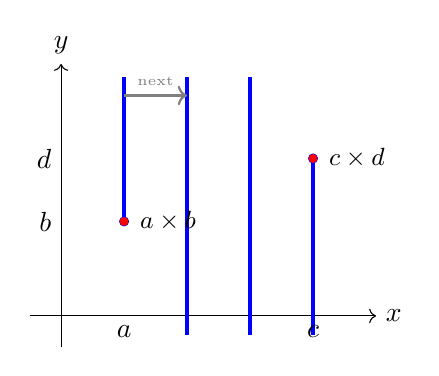
\begin{tikzpicture}[scale=0.8]
    % Axes
    \draw[->] (-0.5,0) -- (5,0) node[right] {$x$};
    \draw[->] (0,-0.5) -- (0,4) node[above] {$y$};
    
    % Shaded region - vertical line at x=a (upper part)
    \draw[very thick, blue] (1,1.5) -- (1,3.8);
    \draw[blue, fill=white] (1,1.5) circle (2pt);
    
    % Shaded region - full vertical lines for a < x < c
    \draw[very thick, blue] (2,-0.3) -- (2,3.8);
    \draw[very thick, blue] (3,-0.3) -- (3,3.8);
    
    % Shaded region - vertical line at x=c (lower part)
    \draw[very thick, blue] (4,-0.3) -- (4,2.5);
    \draw[blue, fill=white] (4,2.5) circle (2pt);
    
    % Points
    \node[below] at (1,0) {$a$};
    \node[below] at (4,0) {$c$};
    \node[left] at (0,1.5) {$b$};
    \node[left] at (0,2.5) {$d$};
    
    % Labels for points
    \fill[red] (1,1.5) circle (2pt);
    \fill[red] (4,2.5) circle (2pt);
    \node[right] at (1.1,1.5) {\small $a \times b$};
    \node[right] at (4.1,2.5) {\small $c \times d$};
    
    % Arrow showing direction
    \draw[->, thick, gray] (1,3.5) to[out=0,in=180] (2,3.5);
    \node[above, gray] at (1.5,3.5) {\tiny next};
\end{tikzpicture}
\end{center}

\textbf{2. Open interval $(a \times b, a \times d)$ on the same vertical line ($b < d$):}

\begin{center}
\begin{tikzpicture}[scale=0.8]
    % Axes
    \draw[->] (-0.5,0) -- (4,0) node[right] {$x$};
    \draw[->] (0,-0.5) -- (0,4) node[above] {$y$};
    
    % Shaded region - segment on vertical line
    \draw[very thick, blue] (2,1) -- (2,3);
    \draw[blue, fill=white] (2,1) circle (2pt);
    \draw[blue, fill=white] (2,3) circle (2pt);
    
    % Points
    \node[below] at (2,0) {$a$};
    \node[left] at (0,1) {$b$};
    \node[left] at (0,3) {$d$};
    
    % Labels
    \fill[red] (2,1) circle (2pt);
    \fill[red] (2,3) circle (2pt);
    \node[right] at (2.1,1) {\small $a \times b$};
    \node[right] at (2.1,3) {\small $a \times d$};
\end{tikzpicture}
\end{center}

\textbf{3. Ray $(a \times b, \infty)$:}

\begin{center}
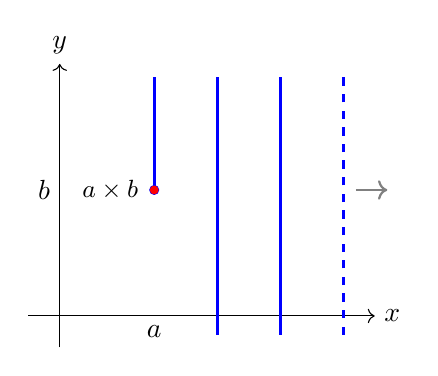
\begin{tikzpicture}[scale=0.8]
    % Axes
    \draw[->] (-0.5,0) -- (5,0) node[right] {$x$};
    \draw[->] (0,-0.5) -- (0,4) node[above] {$y$};
    
    % Shaded region - vertical line at x=a (upper part)
    \draw[very thick, blue] (1.5,2) -- (1.5,3.8);
    \draw[blue, fill=white] (1.5,2) circle (2pt);
    
    % Shaded region - full vertical lines for x > a
    \draw[very thick, blue] (2.5,-0.3) -- (2.5,3.8);
    \draw[very thick, blue] (3.5,-0.3) -- (3.5,3.8);
    \draw[very thick, blue, dashed] (4.5,-0.3) -- (4.5,3.8);
    
    % Point
    \node[below] at (1.5,0) {$a$};
    \node[left] at (0,2) {$b$};
    
    % Label
    \fill[red] (1.5,2) circle (2pt);
    \node[left] at (1.4,2) {\small $a \times b$};
    
    % Arrow to infinity
    \draw[->, thick, gray] (4.7,2) -- (5.2,2);
\end{tikzpicture}
\end{center}

\textbf{4. Ray $(-\infty, c \times d)$:}

\begin{center}
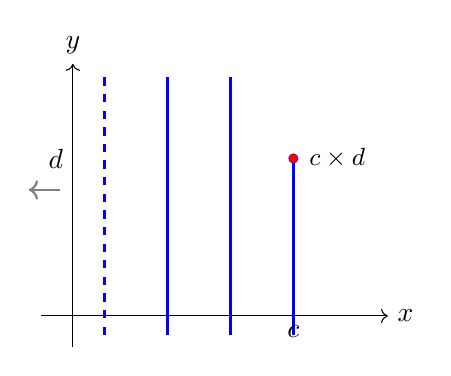
\begin{tikzpicture}[scale=0.8]
    % Axes
    \draw[->] (-0.5,0) -- (5,0) node[right] {$x$};
    \draw[->] (0,-0.5) -- (0,4) node[above] {$y$};
    
    % Shaded region - full vertical lines for x < c
    \draw[very thick, blue, dashed] (0.5,-0.3) -- (0.5,3.8);
    \draw[very thick, blue] (1.5,-0.3) -- (1.5,3.8);
    \draw[very thick, blue] (2.5,-0.3) -- (2.5,3.8);
    
    % Shaded region - vertical line at x=c (lower part)
    \draw[very thick, blue] (3.5,-0.3) -- (3.5,2.5);
    \draw[blue, fill=white] (3.5,2.5) circle (2pt);
    
    % Point
    \node[below] at (3.5,0) {$c$};
    \node[left] at (0,2.5) {$d$};
    
    % Label
    \fill[red] (3.5,2.5) circle (2pt);
    \node[right] at (3.6,2.5) {\small $c \times d$};
    
    % Arrow from infinity
    \draw[<-, thick, gray] (-0.7,2) -- (-0.2,2);
\end{tikzpicture}
\end{center}

\textbf{Key insight:} Unlike the standard topology on $\mathbb{R}^2$ (where open sets are ``blobs''), open sets in the dictionary order topology are unions of vertical line segments and rays. The topology is much finer in the horizontal direction.
\end{exbox}

\subsection{The Order Topology}

\begin{defbox}[Order Topology]
Let $X$ be a set with a simple order relation. Assume $X$ has more than one element. Let $\mathcal{B}$ be the basis consisting of:
\begin{itemize}
    \item Open intervals $(a, b)$, for $a, b \in X$
    \item Intervals $[a_0, b)$, where $a_0$ is the smallest (if any) in $X$
    \item Intervals $(a, b_0]$, where $b_0$ is the largest (if any) in $X$
\end{itemize}
The topology generated by $\mathcal{B}$ is the \textbf{order topology} on $X$.
\end{defbox}

\begin{exbox}
The standard topology on $\mathbb{R}$ is the same as the order topology on $\mathbb{R}$.
\end{exbox}

\begin{exbox}[Order Topology on $\mathbb{Z}_+$]
What is the order topology on $\mathbb{Z}_+ = \{1, 2, 3, \ldots\}$?

The basis $\mathcal{B} = \{(n, m), [1, n)\}$. The basis includes all one-point sets $\{n\}$:
\begin{itemize}
    \item $\{1\} = [1, 2)$
    \item $\{n\} = \{n-1, n+1\} \cap \mathbb{Z}_+ = (n-1, n+1)$ for $n \geq 2$
\end{itemize}
Can form all subsets of $\mathbb{Z}_+$ by finite unions of $\{n\}$'s. $\Rightarrow$ Same as discrete topology.
\end{exbox}

\begin{exbox}[Order Topology on a Product Set]
The set $X = \{1, 2\} \times \mathbb{Z}_+$ with order topology given by dictionary order.

\textbf{Q:} Is there a smallest element in $X$? Largest? Same as discrete?

\textbf{A:} 
\begin{enumerate}
    \item Yes, $1 \times 1$ is the smallest.
    \item No. Assume $a \times b >$ all other elements, so $a = 2$, but there's no largest element in $\mathbb{Z}_+$, so no.
    \item $\{1 \times 1\} = [1 \times 1, 1 \times 2)$. Is $\{2 \times 1\}$ open in the order topology?
\end{enumerate}

Any open set containing $2 \times 1$ must contain a basis element $2 \times 1 \in (i \times a, j \times b)$ for some basis element with $i, j \in \{1, 2\}$.

If $a, b \in \mathbb{Z}_+$: $2 \times 1 \in (1 \times a, 2 \times b) \Rightarrow$ any basis element containing $2 \times 1$ must contain more than one point.

So $\neq$ discrete topology.
\end{exbox}

% ============================================================================
% SECTION 4: PRODUCT TOPOLOGY
% ============================================================================
\section{Product Topology}

\textit{Reference: Munkres Ch 2.15}

\subsection{Definition and Basis}

\begin{defbox}[Product Topology on $X \times Y$]
Let $X, Y$ be topological spaces. The \textbf{product topology} on $X \times Y$ has basis
\[\mathcal{B} = \{U \times V \mid U \subseteq X \text{ open in } X, \; V \subseteq Y \text{ open in } Y\}\]
\end{defbox}

\begin{rembox}[Why This Basis for Products?]
The product topology uses sets $U \times V$ where \emph{each factor is open}---imposing constraints on finitely many coordinates at a time. Why not use arbitrary products of open sets? For two factors this distinction is invisible, but it becomes essential for infinite products (Section 10): the \emph{box topology} imposes constraints on all coordinates simultaneously and behaves pathologically (e.g., $\mathbb{R}^\omega$ in the box topology is not metrizable, and many natural maps fail to be continuous). The product topology, requiring only finitely many coordinate constraints, is the \emph{right} choice: it makes projections continuous, products of compact spaces compact (Tychonoff), and satisfies the universal property that a map into a product is continuous iff each component is.
\end{rembox}

\begin{rembox}[Check that $\mathcal{B}$ is a basis]
\begin{enumerate}
    \item Since $X \times Y \in \mathcal{B}$, every $x \times y \in X \times Y$ belongs to a basis element ($X \times Y$).
    \item If $x \times y \in (U_1 \times V_1) \cap (U_2 \times V_2)$, then $x \times y \in (U_1 \cap U_2) \times (V_1 \cap V_2) \subseteq (U_1 \times V_1) \cap (U_2 \times V_2)$. \checkmark
\end{enumerate}
\end{rembox}

\begin{thmbox}[Basis for Product Topology]
If $\mathcal{B}$ is a basis for the topology on $X$, and $\mathcal{C}$ is a basis for the topology on $Y$, then 
\[\mathcal{D} = \{B \times C \mid B \in \mathcal{B}, C \in \mathcal{C}\}\]
is a basis for the product topology on $X \times Y$.
\end{thmbox}

\begin{proof}
Check $\mathcal{D}$ is a basis:
\begin{enumerate}
    \item If $x \times y \in X \times Y$, then $\exists\, B \in \mathcal{B}$ s.t. $x \in B$, $\exists\, C \in \mathcal{C}$ s.t. $y \in C$. So $x \times y \in B \times C \in \mathcal{D}$.
    \item If $x \times y \in (B_1 \times C_1) \cap (B_2 \times C_2) = (B_1 \cap B_2) \times (C_1 \cap C_2)$. Then $\exists\, B_3 \in \mathcal{B}$ s.t. $x \in B_3 \subseteq B_1 \cap B_2$, and $\exists\, C_3 \in \mathcal{C}$ s.t. $y \in C_3 \subseteq C_1 \cap C_2$. So $x \times y \in B_3 \times C_3 \subseteq (B_1 \times C_1) \cap (B_2 \times C_2)$.
\end{enumerate}

Now we show $\mathcal{D}$ generates the same topology as the product topology. Let $\mathcal{T}_{\text{prod}}$ have basis $\mathcal{B}_{\text{prod}} = \{U \times V \mid U \text{ open in } X, V \text{ open in } Y\}$, and let $\mathcal{T}_{\mathcal{D}}$ be the topology generated by $\mathcal{D}$. By Corollary 2.3:

$(\mathcal{T}_{\mathcal{D}} \subseteq \mathcal{T}_{\text{prod}})$: Each $B \times C \in \mathcal{D}$ is open in $\mathcal{T}_{\text{prod}}$ since $B$ is open in $X$ and $C$ is open in $Y$.

$(\mathcal{T}_{\text{prod}} \subseteq \mathcal{T}_{\mathcal{D}})$: Let $U \times V \in \mathcal{B}_{\text{prod}}$. Since $U = \bigcup_\alpha B_\alpha$ and $V = \bigcup_\beta C_\beta$ for $B_\alpha \in \mathcal{B}$, $C_\beta \in \mathcal{C}$, we have $U \times V = \bigcup_{\alpha, \beta} (B_\alpha \times C_\beta)$, which is a union of elements of $\mathcal{D}$. Thus $U \times V \in \mathcal{T}_{\mathcal{D}}$.

By Corollary 2.3, $\mathcal{T}_{\mathcal{D}} = \mathcal{T}_{\text{prod}}$.
\end{proof}

\begin{exbox}[Standard Topology on $\mathbb{R}^2$]
The product topology on $\mathbb{R} \times \mathbb{R} = \mathbb{R}^2$ is called the \textbf{standard topology} on $\mathbb{R}^2$.

Basis: products of open sets in $\mathbb{R}$. Or another basis: products of open intervals in $\mathbb{R}$.
\[\{(a,b) \times (c,d) \mid a, b, c, d \in \mathbb{R}\}\]
(Note: $\mathbb{R}$ is in standard topology.)
\end{exbox}

\begin{exbox}[Discrete Product Topology]
If $X$ and $Y$ have the discrete topology, what's the product topology on $X \times Y$?

All $\{x\} \subset X$, $\{y\} \subset Y$ $\Rightarrow$ $\{x\} \times \{y\} = \{x \times y\}$ is open in $X \times Y$ $\Rightarrow$ forms every subset of $X \times Y$.

This is the discrete topology on $X \times Y$.
\end{exbox}

\begin{exbox}
(HW2) Order topology on $\mathbb{R} \times \mathbb{R}$ is the same as the product topology on $\mathbb{R}_{\text{discrete}} \times \mathbb{R}_{\text{std}}$.
\end{exbox}

% ============================================================================
% SECTION 5: SUBSPACE TOPOLOGY
% ============================================================================
\section{Subspace Topology}

\textit{Reference: Munkres Ch 2.16}

\subsection{Definition and Basic Properties}

\begin{defbox}[Subspace Topology]
Let $(X, \mathcal{T})$ be a topological space. If $Y \subseteq X$ is a subset, the collection 
\[\mathcal{T}_Y = \{Y \cap U \mid U \in \mathcal{T}\}\]
is a topology on $Y$, called the \textbf{subspace topology}. With this topology, $Y$ is called a \textbf{subspace} of $X$.
\end{defbox}

\begin{rembox}[Why the Subspace Topology?]
The subspace topology is the \emph{unique} topology on $Y$ that makes the inclusion map $\iota: Y \hookrightarrow X$ continuous and satisfies a universal property: a function $f: Z \to Y$ is continuous if and only if $\iota \circ f: Z \to X$ is continuous. In other words, this is the coarsest topology on $Y$ such that ``being a subset'' respects the topological structure. The key subtlety is that open in $Y$ need not be open in $X$---$[0, \tfrac{1}{2})$ is open in $[0,1)$ but not in $\mathbb{R}$. Getting comfortable with this distinction is essential for working with compactness and connectedness in subspaces.
\end{rembox}

\begin{exbox}
$[0,1) \subseteq \mathbb{R}$. Is $[0, \frac{1}{2}) \subseteq \mathbb{R}$ open in $\mathbb{R}$? No. If $0 \in B \in \mathcal{B}$, then $B \subseteq [0, \frac{1}{2})$ is impossible since $B$ must contain points less than $0$.

Is $[0, \frac{1}{2}) \subseteq [0,1)$ open in $[0,1)$? Yes: $(-1, \frac{1}{2}) \cap [0,1) = [0, \frac{1}{2})$, which is open in $[0,1)$.
\end{exbox}

\begin{lembox}[Basis for Subspace Topology]
If $\mathcal{B}$ is a basis for the topology of $X$, then $\mathcal{B}_Y = \{B \cap Y \mid B \in \mathcal{B}\}$ is a basis for the subspace topology on $Y$.
\end{lembox}

\begin{lembox}
If $Y \subseteq X$, $U$ is open in $Y$, and $Y$ is open in $X$, then $U$ is open in $X$.
\end{lembox}

\begin{proof}
$U$ open in $Y$ $\Rightarrow$ $U = V \cap Y$ where $V$ is open in $X$. $\Rightarrow$ $U$ is open in $X$ since $V$ and $Y$ are both open in $X$.

$Y$ open in $X$ $\Rightarrow$ $V \cap Y$ is open in $X$.
\end{proof}

\begin{exbox}
$Y = [0,1] \subseteq X = \mathbb{R}$. The subspace topology on $Y$ has basis $\{(a,b) \cap Y \mid a, b \in \mathbb{R}\}$:
\begin{itemize}
    \item $(a,b)$ if $a, b \in Y$
    \item $[0, b)$ if $b \in Y$, $a \notin Y$
    \item $(a, 1]$ if $a \in Y$, $b \notin Y$
    \item $\emptyset$ if $a, b \notin Y$
\end{itemize}
For $[0,1] \subseteq \mathbb{R}$, the subspace topology is the same as the order topology on $[0,1]$.
\end{exbox}

\begin{exbox}[Subspace $\neq$ Order Topology: $I \times I$]
Consider $[0,1] \times [0,1] \subseteq \mathbb{R} \times \mathbb{R}$ with dictionary order. The subspace topology on $I \times I$ is \textbf{not} the same as the order topology on $I \times I$.

Consider $\{\frac{1}{2}\} \times (\frac{1}{2}, 1]$. 

$\mathcal{D}$: $\{\frac{1}{2}\} \times (\frac{1}{2}, 1]$ is open in subspace topology: $= U \cap (I \times I)$, where $U = (\frac{1}{2} - \frac{1}{2}, \frac{1}{2} + \frac{1}{2}) \times (\frac{1}{2}, 2) \subseteq \mathbb{R} \times \mathbb{R}$.

$\mathcal{D}$: $\{\frac{1}{2}\} \times (\frac{1}{2}, 1]$ not open in order topology on $I \times I$. The point $\frac{1}{2} \times 1$ is not a max in $I \times I$, so any basis element containing $\frac{1}{2} \times 1$ must contain some $p \times q > \frac{1}{2} \times 1$. But for $\frac{1}{2} \times 1 \in \mathcal{B} \subseteq \{\frac{1}{2}\} \times (\frac{1}{2}, 1]$, we would need $\mathcal{B}$ to contain only points with first coordinate $\frac{1}{2}$, which contradicts containing points greater than $\frac{1}{2} \times 1$.
\end{exbox}

% ============================================================================
% CHAPTER 2
% ============================================================================
\chapter{Closedness, Continuity, and Hausdorff}

% ============================================================================
% SECTION 6: CLOSED SETS AND LIMIT POINTS
% ============================================================================
\section{Closed Sets and Limit Points}

\subsection{Closed Sets}

\begin{defbox}[Closed Set]
A subset $A \subseteq X$ is \textbf{closed} if $X \setminus A$ is open.
\end{defbox}

\begin{exbox}
$[a, b] \subseteq \mathbb{R}$ is closed.
\end{exbox}

\begin{exbox}
$\{x \times y \in \mathbb{R}^2 \mid x \leq 0 \text{ and } y \leq 0\} \subseteq \mathbb{R}^2$ is closed.

Its complement is the union of two open sets: $\mathbb{R} \times (0, \infty) \cup (0, \infty) \times \mathbb{R}$.
\end{exbox}

\begin{exbox}
In the discrete topology on a set $X$, every set $X \setminus A$ is open $\Rightarrow$ every subset $A \subseteq X$ is closed.
\end{exbox}

\begin{exbox}
$Y = [0,1] \cup (2,3) \subseteq \mathbb{R}$ with subspace topology.

$[0,1]$ is closed in $Y$ since its complement $(2,3)$ is open in $Y$.

$(2,3)$: $(-1, 2) \cap Y = [0,1]$ is open in $Y$, so $(2,3)$ is closed.
\end{exbox}

\begin{thmbox}[Properties of Closed Sets]
Let $X$ be a topological space.
\begin{enumerate}
    \item $\emptyset$ and $X$ are closed.
    \item Arbitrary intersections of closed sets are closed. (If $Z_\alpha$ is closed for each $\alpha \in A$, then $\bigcap_{\alpha \in A} Z_\alpha$ is closed.)
    \item Finite unions of closed sets are closed. (If $Z_1, \ldots, Z_n$ are closed, then $Z_1 \cup \cdots \cup Z_n$ is closed.)
\end{enumerate}
\end{thmbox}

\begin{proof}
\begin{enumerate}
    \item $X \setminus X = \emptyset$ is open, $X \setminus \emptyset = X$ is open.
    \item $\bigcap_{\alpha \in A} Z_\alpha = \bigcap_{\alpha} (X \setminus U_\alpha) = X \setminus \left(\bigcup_{\alpha \in A} U_\alpha\right)$ is closed, where $U_\alpha = X \setminus Z_\alpha$ is open.
    \item $Z_1 \cup \cdots \cup Z_n = X \setminus \left(\bigcap_{i=1}^n (X \setminus Z_i)\right)$. Since each $X \setminus Z_i$ is open, and finite intersections of open sets are open, the complement is closed.
\end{enumerate}
\end{proof}

\subsection{Closed Sets in Subspaces}

\begin{thmbox}[Closed Sets in Subspaces]
Let $Y \subseteq X$ (subspace). Then $A \subseteq Y$ is closed in $Y$ if and only if $A$ equals the intersection of a closed set of $X$ with $Y$.
\end{thmbox}

\begin{proof}
$(\Leftarrow)$ Suppose $A = C \cap Y$, where $C$ is closed in $X$. Then $Y \setminus A = Y \setminus (C \cap Y) = (X \setminus C) \cap Y$, which is open in $Y$. Hence $A$ is closed in $Y$.

$(\Rightarrow)$ Suppose $A$ is closed in $Y$. Then $Y \setminus A$ is open in $Y$, so $Y \setminus A = Y \cap U$ for some $U$ open in $X$. Now:
\[A = Y \setminus (Y \setminus A) = Y \setminus (Y \cap U) = Y \cap (Y \cap U)^c = Y \cap (Y^c \cup U^c) = Y \cap U^c = Y \cap (X \setminus U)\]
Since $U$ is open in $X$, $X \setminus U$ is closed in $X$. Thus $A = Y \cap (\text{closed set in } X)$.

\textit{Remark on notation:} Here $B^c$ denotes the complement of $B$ in the ambient space $X$, so $A \setminus B = A \cap B^c$. The key step $Y \cap (Y^c \cup U^c) = Y \cap U^c$ follows since $Y \cap Y^c = \emptyset$.
\end{proof}

\begin{thmbox}
Let $Y \subseteq X$ be a subspace. If $A$ is closed in $Y$, and $Y$ is closed in $X$, then $A$ is closed in $X$.
\end{thmbox}

\begin{proof}
By Theorem 6.3, $A = C \cap Y$ for some $C$ closed in $X$. Since $C$ and $Y$ are both closed in $X$, their intersection $A = C \cap Y$ is closed in $X$.
\end{proof}

% ============================================================================
% SECTION 7: INTERIOR AND CLOSURE
% ============================================================================
\section{Interior and Closure}

\subsection{Definitions}

\begin{defbox}[Interior and Closure]
Let $A \subseteq X$, where $X$ is a topological space.

The \textbf{interior} of $A$, denoted $\text{Int}(A)$ or $\mathring{A}$, is the union of all open sets in $X$ contained in $A$.

The \textbf{closure} of $A$, denoted $\text{cl}(A)$ or $\overline{A}$, is the intersection of all closed sets in $X$ containing $A$.
\end{defbox}

\begin{lembox}[Interior and Closure Containment]
Let $A \subseteq X$ be a subset of a topological space. Then:
\begin{enumerate}
    \item $\text{Int}(A) \subseteq A \subseteq \overline{A}$
    \item If $A$ is open, then $\text{Int}(A) = A$.
    \item If $A$ is closed, then $\overline{A} = A$.
\end{enumerate}
\end{lembox}

\begin{proof}
(1) $\text{Int}(A) \subseteq A$: By definition, $\text{Int}(A)$ is the union of all open sets contained in $A$. If $x \in \text{Int}(A)$, then $x \in U$ for some open $U \subseteq A$, hence $x \in A$.

$A \subseteq \overline{A}$: By definition, $\overline{A}$ is the intersection of all closed sets containing $A$. Every such closed set contains $A$, so their intersection contains $A$.

(2) If $A$ is open, then $A$ is an open set contained in $A$, so $A \subseteq \text{Int}(A)$. Combined with (1), $\text{Int}(A) = A$.

(3) If $A$ is closed, then $A$ is a closed set containing $A$, so $\overline{A} \subseteq A$. Combined with (1), $\overline{A} = A$.
\end{proof}

\begin{rembox}
$\text{Int}(A)$ is open in $X$. $\overline{A}$ is closed in $X$.
\end{rembox}

\begin{rembox}[Intuition: Room to Wiggle and Reachable by Limits]
Think of $\text{Int}(A)$ as the points where you have ``room to wiggle''---you can perturb slightly in any direction and stay in $A$. The closure $\overline{A}$ consists of points ``reachable by limits'' from $A$: if every neighborhood of $x$ meets $A$, then $x \in \overline{A}$ (this is made precise by Theorem 7.3 below). The boundary $\overline{A} \setminus \text{Int}(A)$ is the ``edge''---points that are reachable from $A$ but have no wiggle room.

This duality ($\text{Int}$ expands from inside, $\overline{\phantom{A}}$ approaches from outside) is formalized by the identity $X \setminus \text{Int}(A) = \overline{X \setminus A}$: the complement of the interior is the closure of the complement.
\end{rembox}

\begin{exbox}
$A = [0, 1] \subseteq \mathbb{R}$. Then $\text{Int}(A) = (0, 1)$ and $\overline{A} = [0, 1]$.
\end{exbox}

\begin{rembox}
If $A \subset Y \subseteq X$ (where $Y$ is a subspace), closure and interior in $Y$ may differ from closure and interior in $X$. Need to clarify which space we're working in.
\end{rembox}

\subsection{Closure in Subspaces}

\begin{thmbox}[Closure in Subspace]
Let $Y \subseteq X$ be a subspace of $X$, $A \subseteq Y$, $\overline{A}$ = closure of $A$ in $X$. Then the closure of $A$ in $Y$ is equal to $\overline{A} \cap Y$.
\end{thmbox}

\begin{proof}
Let $B$ be the closure of $A$ in $Y$.

$(\supseteq)$ $\overline{A}$ is closed in $X$ $\Rightarrow$ $\overline{A} \cap Y$ is closed in $Y$. Since $\overline{A} \supseteq A$, and by definition, $B$ is the intersection of all closed sets of $Y$ containing $A$, $\Rightarrow$ $B \subseteq \overline{A} \cap Y$.

$(\subseteq)$ $B$ closed in $Y$ $\Rightarrow$ $B = C \cap Y$, where $C$ is closed in $X$, and $C \supseteq A$ since $B \supseteq A$. Since $\overline{A}$ is the intersection of all such closed sets, $\overline{A} \subseteq C$, thus $\overline{A} \cap Y \subseteq C \cap Y = B$.
\end{proof}

\begin{exbox}
$Y = (0, 1] \subseteq \mathbb{R}$. Let $A = (0, \frac{1}{2}) \subseteq Y$.

The closure of $A$ in $\mathbb{R}$ is $[0, \frac{1}{2}]$.

The closure of $A$ in $Y$ is $[0, \frac{1}{2}] \cap Y = (0, \frac{1}{2}]$.
\end{exbox}

\subsection{Neighborhoods}

\begin{defbox}[Intersects and Neighborhood]
We say a set $A$ \textbf{intersects} a set $B$ if $A \cap B \neq \emptyset$.

If $U \subseteq X$ is an open set containing $x \in X$, we say ``$U$ is a \textbf{neighborhood} of $x$''.
\end{defbox}

\begin{exbox}
$(-\varepsilon, \varepsilon)$ is a neighborhood of $0$ in $\mathbb{R}$.
\end{exbox}

\subsection{Closure via Neighborhoods}

\begin{thmbox}[Closure Characterization]
Let $A \subseteq X$ be a subset of a topological space. Then $x \in \overline{A}$ if and only if every neighborhood of $x$ intersects $A$.
\end{thmbox}

\begin{proof}
$(\Rightarrow)$ If $x \notin \overline{A}$, then $x \in X \setminus \overline{A}$, which is open in $X$ (since $\overline{A}$ is closed). So $X \setminus \overline{A}$ is a neighborhood of $x$ that doesn't intersect $A$. Equivalently, if every neighborhood of $x$ intersects $A$, then $x \in \overline{A}$.

$(\Leftarrow)$ Conversely, suppose there exists a neighborhood $U$ of $x$ such that $U \cap A = \emptyset$. Then $X \setminus U$ is a closed set containing $A$. By definition of $\overline{A}$, $X \setminus U$ must contain $\overline{A}$. But we know $x \in U$, so $x \notin \overline{A}$.
\end{proof}

\subsection{Limit Points}

\begin{defbox}[Limit Point]
Let $A \subseteq X$, where $X$ is a topological space, and let $x \in X$. We say $x$ is a \textbf{limit point} (or \textbf{accumulation point}, \textbf{cluster point}) of $A$ if every neighborhood of $x$ intersects $A$ in some point other than $x$. That is, $x$ is a limit point if $x \in \overline{A \setminus \{x\}}$.
\end{defbox}

\begin{exbox}
In $\mathbb{R}$, let $B = \{\frac{n+1}{n} \mid n \in \mathbb{Z}_+\}$. What are the limit points of $B$?

$1 \in \mathbb{R}$ is a limit point.
\end{exbox}

\begin{exbox}
$(0,1)$: What are the limit points? Every point in $[0,1]$ is a limit point of $A$.
\end{exbox}

\begin{exbox}
$\mathbb{Q} \subseteq \mathbb{R}$? Any $x \in \mathbb{R}$! Because $\mathbb{Q}$ is dense in $\mathbb{R}$. $(x - \varepsilon, x + \varepsilon)$ contains some $q \in \mathbb{Q}$.
\end{exbox}

\begin{thmbox}[Closure and Limit Points]
Let $A \subseteq X$ be a subset of a topological space. Let $A'$ = set of all limit points of $A$. Then $\overline{A} = A \cup A'$.
\end{thmbox}

\begin{proof}
$(\supseteq)$ If $x \in A'$, then every neighborhood of $x$ intersects $A$. $\Rightarrow$ $x \in \overline{A}$. If $x \in A \Rightarrow x \in \overline{A}$. \checkmark

$(\subseteq)$ Let $x \in \overline{A}$. If $x \in A$, then done. If $x \notin A$, then every neighborhood of $x$ intersects $A$ (since $x \in \overline{A}$), and that intersected point is not $x$, so $x \in A'$. \checkmark
\end{proof}

\begin{corbox}
$A \subseteq X$ (topological space) is closed if and only if $A$ contains all of its limit points.
\end{corbox}

\begin{proof}
$A$ closed $\Leftrightarrow$ $A = \overline{A} \Leftrightarrow A \supseteq A'$.
\end{proof}

\begin{exbox}[Strange Behavior]
$X = \{a, b, c\}$ with topology $\{\{b\}, \{a,b\}, \{b,c\}, X, \emptyset\}$. Note $\{b\}$ is not closed (its complement $\{a,c\}$ is not open).
\end{exbox}

\subsection{Convergence of Sequences}

\begin{defbox}[Convergence]
Let $\{x_n\}$ be a sequence of points in $X$. We say $x_n \to x$ (``$x_n$ converges to $x$'') if for every neighborhood $U$ of $x$, there is some $N \in \mathbb{Z}$ such that $x_n \in U$ for all $n \geq N$.
\end{defbox}

\begin{exbox}
$x_n = b \to a, b, c$ in the space $X = \{a,b,c\}$ above, since every neighborhood of $a$ contains $b$, same for $b$ and $c$.
\end{exbox}

% ============================================================================
% SECTION 8: HAUSDORFF SPACES
% ============================================================================
\section{Hausdorff Spaces}

\begin{defbox}[Hausdorff Space]
A topological space $X$ is called \textbf{Hausdorff} (or $T_2$) if for each pair $x_1$ and $x_2$ of distinct points in $X$, there exist neighborhoods $U_1$ of $x_1$ and $U_2$ of $x_2$ that are disjoint.
\end{defbox}

\begin{rembox}[Why Hausdorff is the ``Reasonable'' Separation Axiom]
The Hausdorff property is the minimal assumption that makes a topological space behave like what we expect from analysis:
\begin{itemize}
    \item \textbf{Unique limits:} sequences (and nets) converge to at most one point.
    \item \textbf{Points are closed:} single-point sets $\{x\}$ are closed ($T_1$).
    \item \textbf{Compact subsets are closed:} compact $\subseteq$ Hausdorff $\Rightarrow$ closed (Theorem 15.4).
    \item \textbf{Bijections behave:} continuous bijections from compact to Hausdorff are homeomorphisms.
\end{itemize}
Without Hausdorff, pathologies arise: in the cofinite topology on $\mathbb{R}$, every sequence with distinct terms converges to \emph{every} point. Most spaces in practice are Hausdorff (metric spaces, manifolds, CW complexes), and the separation axiom hierarchy (Section 19) refines this further.
\end{rembox}

\begin{exbox}
In $\mathbb{R}$: Given $x \neq y$, take $U_x = (x - \varepsilon, x + \varepsilon)$ and $U_y = (y - \varepsilon, y + \varepsilon)$ where $\varepsilon = \frac{|x-y|}{3}$. These are disjoint.

Counter-example: The cofinite topology on $\mathbb{R}$ is not Hausdorff.
\end{exbox}

\begin{thmbox}[Finite Point Sets are Closed in Hausdorff Spaces]
Every finite point set in a Hausdorff space is closed.
\end{thmbox}

\begin{proof}
It suffices to show every one-point set $\{x_0\}$ is closed. Show $X \setminus \{x_0\}$ is open. Let $y \in X \setminus \{x_0\}$. Since $X$ is Hausdorff, there exist disjoint neighborhoods $U_x$ of $x_0$ and $U_y$ of $y$ with $U_x \cap U_y = \emptyset$. $\Rightarrow$ $X \setminus \{x_0\} = \bigcup_{y \in X \setminus \{x_0\}} U_y$ is a union of open sets $\Rightarrow$ open.

(Note: each $U_y \subseteq X \setminus \{x_0\}$, and each $y \in X \setminus \{x_0\}$ is in $U_y$ as well.)
\end{proof}

\begin{propbox}[$T_1$ Axiom]
Let $X$ be a topological space in which finite point sets are closed. We say $X$ satisfies the $T_1$ axiom.

By the theorem, Hausdorff $\Rightarrow$ $T_1$ axiom, but not vice versa (e.g., cofinite topology on $\mathbb{R}$).
\end{propbox}

\begin{thmbox}[Unique Limits in Hausdorff Spaces]
If $X$ is a Hausdorff space, then a sequence of points of $X$ must converge to at most one point of $X$.
\end{thmbox}

\begin{proof}
Let $x_n \to x$. If $y \neq x$, take $U_x, U_y$ neighborhoods of $x, y$ disjoint. Since $U_x$ contains all $x_n$ with $n \geq N_1$ for some $N_1$, but if $U_y$ also contains $x_n$ with $n \geq N_2$ for some $N_2$, then $U_x, U_y$ contains all points where $n \geq \max\{N_1, N_2\}$, contradiction.
\end{proof}

% ============================================================================
% SECTION 9: CONTINUOUS FUNCTIONS
% ============================================================================
\section{Continuous Functions}

\textit{Reference: Munkres Ch 2 \S 18}

\subsection{Definition and Basic Properties}

\begin{defbox}[Continuous Function]
Let $X, Y$ be topological spaces. A function $f: X \to Y$ is \textbf{continuous} if for each open set $V \subseteq Y$, the preimage $f^{-1}(V)$ is a subset of $X$ that is open.

(Generalizes $\varepsilon$-$\delta$ since metric definition.)
\end{defbox}

\begin{proof}[Proof that checking on basis suffices]
It suffices to show the inverse image of every basis element is open. Let $V = \bigcup_\alpha B_\alpha$. Then $f^{-1}(V) = \bigcup_\alpha f^{-1}(B_\alpha)$. If each $f^{-1}(B_\alpha)$ is open, then $f^{-1}(V)$ is open.
\end{proof}

\begin{exbox}[$f: \mathbb{R} \to \mathbb{R}$ in analysis]
The ``$\varepsilon$-$\delta$'' definition of continuous function: $\forall \varepsilon > 0$, w.t.s. $\exists \delta > 0$ s.t. $|f(x) - f(y)| < \varepsilon$ if $|x - y| < \delta$.

Topological definition $\Leftrightarrow$ ``$\varepsilon$-$\delta$'': $\forall x \in \mathbb{R}$, $f^{-1}((f(x) - \varepsilon, f(x) + \varepsilon))$ is an open set in $\mathbb{R}$, i.e., is a neighborhood of $x$.

$\exists \delta > 0$ s.t. $(x - \delta, x + \delta) \subset f^{-1}((f(x) - \varepsilon, f(x) + \varepsilon))$. \checkmark
\end{exbox}

\begin{exbox}[$\mathbb{R}_\ell$: Lower limit topology]
$\mathcal{B}_\ell = \{[a,b) \mid a, b \in \mathbb{R}\}$. $f: \mathbb{R} \to \mathbb{R}$, $f(x) = x$.

\textbf{(1)} $f: \mathbb{R}_{\text{std}} \to \mathbb{R}_\ell$ not continuous. $[a,b)$ open in $\mathbb{R}_\ell$, but $f^{-1}([a,b)) = [a,b)$ not open in $\mathbb{R}_{\text{std}}$.

\textbf{(2)} $f: \mathbb{R}_\ell \to \mathbb{R}$. $f^{-1}((a,b)) = (a,b) = \bigcup_{n=1}^{\infty} [a + \frac{1}{n}, b)$. This is open in $\mathbb{R}_\ell$. So $f$ is continuous.

\textbf{Conclusion:} Continuity depends on $f$, and the topologies on $X$, $Y$.
\end{exbox}

\begin{thmbox}[Equivalent Conditions for Continuity]
Let $f: X \to Y$ be a function between topological spaces. The following are equivalent:
\begin{enumerate}
    \item $f$ is continuous.
    \item For every subset $A$ of $X$, $f(\overline{A}) \subseteq \overline{f(A)}$.
    \item For every closed subset $B$ of $Y$, $f^{-1}(B)$ is closed in $X$.
    \item For each $x \in X$ and each neighborhood $V$ of $f(x)$, there is a neighborhood $U$ of $x$ such that $f(U) \subseteq V$. (Continuity at $x$)
\end{enumerate}
\end{thmbox}

\begin{proof}
$(1) \Rightarrow (4)$: Let $x \in X$ and let $V$ be a neighborhood of $f(x)$. Since $V$ is open and $f$ is continuous, $f^{-1}(V)$ is open in $X$. Since $f(x) \in V$, we have $x \in f^{-1}(V)$. So $U = f^{-1}(V)$ is a neighborhood of $x$, and $f(U) = f(f^{-1}(V)) \subseteq V$.

$(4) \Rightarrow (1)$: Let $V \subseteq Y$ be open. We show $f^{-1}(V)$ is open. Let $x \in f^{-1}(V)$. Then $f(x) \in V$, so $V$ is a neighborhood of $f(x)$. By (4), there exists a neighborhood $U_x$ of $x$ such that $f(U_x) \subseteq V$. This means $U_x \subseteq f^{-1}(V)$. Since $U_x$ is open and contains $x$, we have shown that every point of $f^{-1}(V)$ has an open neighborhood contained in $f^{-1}(V)$. Thus $f^{-1}(V) = \bigcup_{x \in f^{-1}(V)} U_x$ is a union of open sets, hence open.

$(1) \Rightarrow (3)$: Let $B \subseteq Y$ be closed. Then $Y \setminus B$ is open. By (1), $f^{-1}(Y \setminus B) = X \setminus f^{-1}(B)$ is open. Thus $f^{-1}(B)$ is closed.

$(3) \Rightarrow (1)$: Let $V \subseteq Y$ be open. Then $Y \setminus V$ is closed. By (3), $f^{-1}(Y \setminus V) = X \setminus f^{-1}(V)$ is closed. Thus $f^{-1}(V)$ is open.

$(1) \Rightarrow (2)$: Let $A \subseteq X$. We show $f(\overline{A}) \subseteq \overline{f(A)}$. Let $x \in \overline{A}$. We need $f(x) \in \overline{f(A)}$, i.e., every neighborhood of $f(x)$ intersects $f(A)$. Let $V$ be a neighborhood of $f(x)$. By (1), $f^{-1}(V)$ is open, and $x \in f^{-1}(V)$. Since $x \in \overline{A}$, $f^{-1}(V)$ intersects $A$, say at point $a \in f^{-1}(V) \cap A$. Then $f(a) \in V \cap f(A)$, so $V$ intersects $f(A)$.

$(2) \Rightarrow (3)$: Let $B \subseteq Y$ be closed. Let $A = f^{-1}(B)$. By (2), $f(\overline{A}) \subseteq \overline{f(A)} \subseteq \overline{B} = B$ (since $B$ is closed). Thus $\overline{A} \subseteq f^{-1}(B) = A$. Since $A \subseteq \overline{A}$ always, we have $\overline{A} = A$, so $f^{-1}(B)$ is closed.
\end{proof}

\subsection{Homeomorphisms}

\begin{defbox}[Homeomorphism]
Let $f: X \to Y$ be a bijection with inverse $f^{-1}: Y \to X$. If both $f$ and $f^{-1}$ are continuous, then $f$ is called a \textbf{homeomorphism}. $\Leftrightarrow$
\end{defbox}

\begin{propbox}[Equivalent Definition of Homeomorphism]
A bijection $f: X \to Y$ is a homeomorphism if and only if $f(U)$ is open $\Leftrightarrow$ $U$ is open.
\end{propbox}

\begin{proof}
$(\Rightarrow)$ Suppose $f$ is a homeomorphism, i.e., $f$ and $f^{-1}$ are both continuous.

If $U \subseteq X$ is open, then since $f^{-1}: Y \to X$ is continuous and $U$ is open, $(f^{-1})^{-1}(U) = f(U)$ is open in $Y$.

If $f(U) \subseteq Y$ is open, then since $f: X \to Y$ is continuous, $f^{-1}(f(U)) = U$ is open in $X$ (using that $f$ is a bijection).

$(\Leftarrow)$ Suppose $f(U)$ is open $\Leftrightarrow$ $U$ is open.

To show $f$ is continuous: Let $V \subseteq Y$ be open. Then $f(f^{-1}(V)) = V$ is open, so by our assumption, $f^{-1}(V)$ is open. Thus $f$ is continuous.

To show $f^{-1}$ is continuous: Let $U \subseteq X$ be open. Then $(f^{-1})^{-1}(U) = f(U)$ is open by assumption. Thus $f^{-1}$ is continuous.
\end{proof}

\begin{rembox}
Homeomorphisms identify open sets: $U$ is open in $X$ if and only if $f(U)$ is open in $Y$. This is why homeomorphic spaces are considered ``topologically the same.''
\end{rembox}

\begin{rembox}[What Homeomorphism Really Means]
A homeomorphism is the topological notion of ``sameness''---just as isomorphism is for groups or vector spaces. Two homeomorphic spaces are indistinguishable from the perspective of topology: they have the same open sets, the same convergent sequences, the same compact and connected subsets.

This is the precise version of ``rubber sheet geometry'': you can stretch, bend, and deform a space continuously (with a continuous inverse), and topology cannot tell the difference. A coffee mug and a doughnut are homeomorphic; a circle and a line segment are not (removing one point from a circle leaves it connected; removing an interior point from a segment does not).

The central question of topology is: \emph{when are two spaces homeomorphic?} This motivates topological invariants---compactness, connectedness, fundamental groups---properties preserved under homeomorphism that can distinguish non-homeomorphic spaces.
\end{rembox}

\begin{exbox}
$f: \mathbb{R} \to \mathbb{R}$, $f(x) = 3x + 1$. Homeomorphism. $g(y) = \frac{1}{3}(y-1)$. Easily check $g \circ f(x) = x$, $f \circ g(y) = y$.
\end{exbox}

\begin{exbox}
$f: (a,b) \to (0,1)$. $f(x) = (x-a) \cdot \frac{1}{b-a}$. $g(y) = (b-a)y + a$. Homeomorphism.
\end{exbox}

\begin{propbox}[Homeomorphisms Restrict to Subspaces]
Let $f: X \to Y$ be a homeomorphism and $A \subseteq X$. Then $f|_A: A \to f(A)$ is a homeomorphism (with the subspace topologies on $A$ and $f(A)$).
\end{propbox}

\begin{proof}
$f|_A$ is a bijection $A \to f(A)$ (restriction of a bijection to a subset). For continuity: $f|_A$ is the restriction of $f$ to $A$, hence continuous (Rule 4). For the inverse: $(f|_A)^{-1} = (f^{-1})|_{f(A)}$, which is the restriction of $f^{-1}$ to $f(A)$, hence continuous.
\end{proof}

\begin{exbox}[{$\mathbb{C} \cong \mathbb{R}^2$ and the Two Faces of $S^1$}]
Define $\phi: \mathbb{C} \to \mathbb{R}^2$ by $\phi(a + bi) = (a, b)$, with inverse $\phi^{-1}(a, b) = a + bi$.

\textbf{$\phi$ is a homeomorphism.} Both $\mathbb{C}$ and $\mathbb{R}^2$ are metric spaces, with metrics
\[d_{\mathbb{C}}(z_1, z_2) = |z_1 - z_2|, \qquad d_{\mathbb{R}^2}(\mathbf{x}_1, \mathbf{x}_2) = \|\mathbf{x}_1 - \mathbf{x}_2\|.\]
Writing $z_j = a_j + b_j i$, we compute directly:
\[|z_1 - z_2| = |(a_1 - a_2) + (b_1 - b_2)i| = \sqrt{(a_1-a_2)^2 + (b_1-b_2)^2} = \|\phi(z_1) - \phi(z_2)\|.\]
So $d_{\mathbb{R}^2}(\phi(z_1), \phi(z_2)) = d_{\mathbb{C}}(z_1, z_2)$ for all $z_1, z_2$. This means $\phi$ is continuous: given $\varepsilon > 0$, take $\delta = \varepsilon$; then $d_{\mathbb{C}}(z_1, z_2) < \delta$ implies $d_{\mathbb{R}^2}(\phi(z_1), \phi(z_2)) < \varepsilon$. The same $\delta = \varepsilon$ argument applies to $\phi^{-1}$. Since $\phi$ is a continuous bijection with continuous inverse, it is a homeomorphism.

\textbf{Restricting to $S^1$.} Since $|z| = 1 \iff a^2 + b^2 = 1$, we have $\phi(S^1_{\mathbb{C}}) = S^1_{\mathbb{R}^2}$. By the restriction proposition, $\phi|_{S^1}: S^1_{\mathbb{C}} \to S^1_{\mathbb{R}^2}$ is a homeomorphism.

This is why we freely write $S^1$ without specifying the ambient space. In particular, the covering map $p(x) = e^{2\pi i x} \in \mathbb{C}$ and $p(x) = (\cos 2\pi x, \sin 2\pi x) \in \mathbb{R}^2$ are the same map under this identification.

\textbf{Consequence for $\pi_1$:} Once we compute $\pi_1(S^1_{\mathbb{R}^2}) \cong \mathbb{Z}$ (via the covering map $p: \mathbb{R} \to S^1_{\mathbb{R}^2}$ in \S 25), we get $\pi_1(S^1_{\mathbb{C}}) \cong \mathbb{Z}$ for free: the homeomorphism $\phi$ induces an isomorphism $\phi_*: \pi_1(S^1_{\mathbb{C}}) \to \pi_1(S^1_{\mathbb{R}^2})$ (\S 23, ``$\pi_1$ is a topological invariant''), so $\pi_1(S^1_{\mathbb{C}}) \cong \pi_1(S^1_{\mathbb{R}^2}) \cong \mathbb{Z}$. No separate computation needed.
\end{exbox}

\subsection{Rules for Constructing Continuous Functions}

\begin{thmbox}[Rules for Continuous Functions]
\begin{enumerate}
    \item (Constant) Constant functions are continuous: $f(x) = c$.
    \item (Inclusion) If $A \subseteq X$, the inclusion $f: A \to X$ is continuous.
    \item (Composition) Compositions of continuous functions are continuous: $f \circ g$ is continuous if $f, g$ are continuous.
    \item (Restriction) Restricting the domain: $f$ continuous $\Rightarrow$ $f|_A$ continuous.
    \item (Restriction/Expansion on range) $f: X \to Y$ continuous, $Z$ a subspace of $Y$, or $Y$ subspace of $Z$. $h: X \to Z$ continuous if $f|_{\text{restricted}}$ continuous.
    \item (Local formulation of continuity) If $X = \bigcup U_\alpha$ (open in $X$), if $f|_{U_\alpha}$ continuous, then $f$ is continuous.
\end{enumerate}
\end{thmbox}

\begin{thmbox}[Pasting Lemma]
Let $X = A \cup B$, $A, B$ closed. $f: A \to Y$, $g: B \to Y$ continuous, and they agree on $A \cap B$.

Then $h(x) = \begin{cases} f(x) & x \in A \\ g(x) & x \in B \end{cases}$ is continuous.
\end{thmbox}

\begin{proof}
We use criterion (3): $h$ is continuous iff the preimage of every closed set is closed.

Let $C \subseteq Y$ be closed. We show $h^{-1}(C)$ is closed in $X$.

Note that $h^{-1}(C) = \{x \in X : h(x) \in C\} = \{x \in A : f(x) \in C\} \cup \{x \in B : g(x) \in C\} = f^{-1}(C) \cup g^{-1}(C)$.

Since $f: A \to Y$ is continuous and $C$ is closed in $Y$, $f^{-1}(C)$ is closed in $A$. Since $A$ is closed in $X$, by Theorem 6.4, $f^{-1}(C)$ is closed in $X$.

Similarly, $g^{-1}(C)$ is closed in $B$, and since $B$ is closed in $X$, $g^{-1}(C)$ is closed in $X$.

Thus $h^{-1}(C) = f^{-1}(C) \cup g^{-1}(C)$ is a finite union of closed sets, hence closed in $X$.
\end{proof}

\begin{exbox}
$f_1: [0, \infty) \to \mathbb{R}$, $f_1(x) = x$. $f_2: (-\infty, 0] \to \mathbb{R}$, $f_2(x) = -x$. (Both continuous.) $\Rightarrow$ $f(x) = |x|$ continuous.
\end{exbox}

% ============================================================================
% CHAPTER 3
% ============================================================================
\chapter{Products, Metrics, and Quotients}

% ============================================================================
% SECTION 10: PRODUCT TOPOLOGY (ARBITRARY PRODUCTS)
% ============================================================================
\section{Product Topology on Arbitrary Products}

\textit{Reference: Munkres Ch 2 \S 19}

\subsection{Definition and Basis}

\begin{defbox}[Product Topology on Arbitrary Products]
The \textbf{product topology} on $\prod_{\alpha \in J} X_\alpha$, where each $X_\alpha$ is a topological space, is the topology with basis consisting of all subsets of the form $\prod_{\alpha \in J} U_\alpha$, where:
\begin{itemize}
    \item $U_\alpha \subseteq X_\alpha$ is open for each $\alpha$
    \item $U_\alpha = X_\alpha$ for all but finitely many $\alpha$ (i.e., at most finitely many $U_\alpha$ are proper subsets of $X_\alpha$)
\end{itemize}
\end{defbox}

\begin{rembox}[Checking the Basis Axioms]
(1) Given $x \in \prod X_\alpha$, $x$ is contained in $\prod U_\alpha$ where all $U_\alpha = X_\alpha$.

(2) If $x \in (\prod U_\alpha) \cap (\prod V_\alpha) = \prod (U_\alpha \cap V_\alpha)$, this is again a basis element. 

\textit{Justification:} Suppose finitely many of the $U_\alpha$ and finitely many of the $V_\alpha$ are proper subsets of $X_\alpha$. We claim that $U_\alpha \cap V_\alpha$ is a proper subset of $X_\alpha$ only if $U_\alpha$ or $V_\alpha$ is a proper subset of $X_\alpha$. (Contrapositive: if both $U_\alpha = X_\alpha$ and $V_\alpha = X_\alpha$, then $U_\alpha \cap V_\alpha = X_\alpha$.)

Thus:
\[\{\alpha \mid U_\alpha \cap V_\alpha \subsetneq X_\alpha\} = \{\alpha \mid U_\alpha \subsetneq X_\alpha \text{ or } V_\alpha \subsetneq X_\alpha\} \subseteq \{\alpha \mid U_\alpha \subsetneq X_\alpha\} \cup \{\alpha \mid V_\alpha \subsetneq X_\alpha\}\]
which is a union of two finite sets, hence finite. So $\prod(U_\alpha \cap V_\alpha)$ satisfies the product basis criteria.
\end{rembox}

\subsection{Continuity and Product Topology}

\begin{thmbox}[Continuity into Product Spaces]
Let $A$ be a topological space. Let $f: A \to \prod_{\alpha \in J} X_\alpha$ be given by $f(a) = (f_\alpha(a))_{\alpha \in J}$, where $f_\alpha: A \to X_\alpha$ is a map. Then $f$ is continuous if and only if $f_\alpha$ is continuous for all $\alpha \in J$.
\end{thmbox}

\begin{proof}
$(\Rightarrow)$ Let $\pi_\beta: \prod X_\alpha \to X_\beta$ be the projection to the $\beta$-factor: $(x_\alpha)_{\alpha \in J} \mapsto x_\beta$.

\textbf{Claim:} $\pi_\beta$ is a continuous map.

\textit{Proof of claim:} Let $U_\beta \subseteq X_\beta$ be an open set. Then $\pi_\beta^{-1}(U_\beta) = \prod_{\alpha \in J} X_\alpha \times U_\beta$, which is open in the product topology (it's a basis element with $U_\alpha = X_\alpha$ for $\alpha \neq \beta$).

Note $f_\beta = \pi_\beta \circ f$, a composition of continuous maps, hence continuous.

$(\Leftarrow)$ Suppose $f_\alpha$ is continuous for all $\alpha \in J$. To show $f$ is continuous, it suffices to show $f^{-1}(\prod_{\alpha \in J} U_\alpha)$ is open in $A$, where $\prod U_\alpha$ is a basis element for the product topology.

Note: $U_\alpha = X_\alpha$ for all but finitely many $\alpha$, say $\alpha_1, \ldots, \alpha_n$.

\[f^{-1}\left(\prod_{\alpha \in J} U_\alpha\right) = \bigcap_{\alpha \in J} f_\alpha^{-1}(U_\alpha) = f_{\alpha_1}^{-1}(U_{\alpha_1}) \cap \cdots \cap f_{\alpha_n}^{-1}(U_{\alpha_n})\]

(Since if $U_\alpha = X_\alpha$, then $f_\alpha^{-1}(U_\alpha) = A$.)

Each $f_{\alpha_i}^{-1}(U_{\alpha_i})$ is open because $f_{\alpha_i}$ is continuous, so this is a finite intersection of open sets in $A$, hence open.
\end{proof}

\begin{exbox}[$\mathbb{R}^\omega$]
Define $\mathbb{R}^\omega = \mathbb{R} \times \mathbb{R} \times \cdots = \prod_{n \in \mathbb{Z}_{>0}} X_n$, where $X_n = \mathbb{R}$.

Let $f: \mathbb{R} \to \mathbb{R}^\omega$ given by $f(t) = (t, t, \ldots, \ldots)$. This is continuous when we endow $\mathbb{R}^\omega$ with product topology because $f_n(t) = t$ is continuous for each $n$.
\end{exbox}

\subsection{Box Topology}

\begin{defbox}[Box Topology]
The \textbf{box topology} on $\prod_{\alpha \in J} X_\alpha$ is the topology with basis given by $\prod_{\alpha \in J} U_\alpha$, where $U_\alpha \subseteq X_\alpha$ is open (with no finiteness restriction).
\end{defbox}

\begin{rembox}
The box topology is in general strictly finer than the product topology (i.e., has more open sets). This causes various pathologies.
\end{rembox}

\begin{rembox}[Why the Product Topology is ``Right'']
The box topology might seem more natural (open in each factor $\Rightarrow$ open in the product), but it is the \emph{product topology} that satisfies the universal property: $f: Z \to \prod X_\alpha$ is continuous iff each $\pi_\alpha \circ f$ is continuous. The example above shows this fails for the box topology---the diagonal map $t \mapsto (t, t, \ldots)$ into $\mathbb{R}^\omega$ is continuous componentwise but not in the box topology.

The product topology also gives us Tychonoff's theorem (arbitrary products of compact spaces are compact), one of the most powerful results in topology. This fails for the box topology. The lesson: imposing only finitely many constraints at a time is what makes infinite products manageable.
\end{rembox}

\begin{exbox}[$f: \mathbb{R} \to \mathbb{R}^\omega$ Not Continuous in Box Topology]
The map $f: \mathbb{R} \to \mathbb{R}^\omega$, $f(t) = (t, t, \ldots)$ is \textbf{not} continuous when $\mathbb{R}^\omega$ is endowed with the box topology.

Consider $U = \prod_{n \in \mathbb{Z}_{>0}} \left(-\frac{1}{n}, \frac{1}{n}\right) = (-1, 1) \times \left(-\frac{1}{2}, \frac{1}{2}\right) \times \cdots \subseteq \mathbb{R}^\omega$, which is open in the box topology.

But $f^{-1}(U) = \bigcap_{n=1}^{\infty} \left(-\frac{1}{n}, \frac{1}{n}\right) = \{0\}$, which is not open in $\mathbb{R}$.
\end{exbox}

% ============================================================================
% SECTION 11: METRIC TOPOLOGY
% ============================================================================
\section{Metric Topology}

\textit{Reference: Munkres Ch 3 \S 20}

\subsection{Metrics and Metric Spaces}

\begin{defbox}[Metric]
A \textbf{metric} on a set $X$ is a function $d: X \times X \to \mathbb{R}$ satisfying:
\begin{enumerate}
    \item $d(x, y) \geq 0$ for all $x, y \in X$, and $d(x, y) = 0 \Leftrightarrow x = y$.
    \item $d(x, y) = d(y, x)$ for all $x, y \in X$. (Symmetry)
    \item $d(x, y) \leq d(x, z) + d(z, y)$ for all $x, y, z \in X$. (Triangle inequality)
\end{enumerate}
\end{defbox}

\begin{exbox}[Euclidean Metric on $\mathbb{R}^n$]
$x = (x_1, \ldots, x_n), y = (y_1, \ldots, y_n) \in \mathbb{R}^n$.
\[d(x, y) = \sqrt{\sum_{i=1}^{n} (x_i - y_i)^2}\]
\end{exbox}

\begin{exbox}[Square Metric on $\mathbb{R}^n$]
\[\rho(x, y) = \max\{|x_1 - y_1|, |x_2 - y_2|, \ldots, |x_n - y_n|\}\]
\end{exbox}

\subsection{$\varepsilon$-Balls and the Metric Topology}

\begin{defbox}[$\varepsilon$-Ball]
Given a metric $d$ on $X$, $x \in X$, $\varepsilon > 0$, the \textbf{$\varepsilon$-ball centered at $x$} is
\[B_d(x, \varepsilon) = \{y \in X \mid d(y, x) < \varepsilon\} \subseteq X\]
\end{defbox}

\begin{defbox}[Metric Topology]
If $d$ is a metric on $X$, then the collection of all $\varepsilon$-balls $B_d(x, \varepsilon)$, $x \in X$, $\varepsilon > 0$, is a basis for a topology on $X$, called the \textbf{metric topology} induced by $d$.
\end{defbox}

\begin{proof}[Proof that $\varepsilon$-balls form a basis]
We check the basis axioms.

(1) If $x \in X$, then $x \in B_d(x, \varepsilon)$ for any $\varepsilon > 0$. \checkmark

(2) Let $y \in B_d(x_1, \varepsilon_1) \cap B_d(x_2, \varepsilon_2)$. We need to find $\delta > 0$ such that $B_d(y, \delta) \subseteq B_d(x_1, \varepsilon_1) \cap B_d(x_2, \varepsilon_2)$.

Let $\delta_1 = \varepsilon_1 - d(y, x_1) > 0$ and $\delta_2 = \varepsilon_2 - d(y, x_2) > 0$. Set $\delta = \min(\delta_1, \delta_2)$.

\textbf{Claim:} $B_d(y, \delta) \subseteq B_d(x_1, \varepsilon_1)$ (similar for $B_d(x_2, \varepsilon_2)$).

\textit{Proof:} Let $z \in B_d(y, \delta)$. Then 
\[d(x_1, z) \leq d(x_1, y) + d(y, z) < d(x_1, y) + \delta_1 = d(x_1, y) + \varepsilon_1 - d(y, x_1) = \varepsilon_1\]

Similarly for $B_d(x_2, \varepsilon_2) \supseteq B_d(y, \delta)$. So $\mathcal{B}_d$ is indeed a basis.
\end{proof}

\subsection{Examples of Metric Spaces}

\begin{exbox}[Euclidean Metric Induces Standard Topology]
$\mathbb{R}^n$, $d(x,y) = \|x - y\| = \left(\sum_{i=1}^{n}(x_i - y_i)^2\right)^{1/2}$ induces the standard topology.
\end{exbox}

\begin{exbox}[Discrete Metric]
$X$ any set. Define $d(x,y) = \begin{cases} 0 & x = y \\ 1 & x \neq y \end{cases}$. This induces the discrete topology.

(Since every singleton $\{x\} = B(x, \frac{1}{2})$ is open.)
\end{exbox}

\begin{exbox}[Sup-Metric on $\mathbb{R}^n$]
$\rho(x,y) = \max_i\{|x_i - y_i|\}$, the ``sup-metric.''
\end{exbox}

\subsection{Comparing Metric Topologies}

\begin{lembox}[Comparing Metric Topologies]
Let $d$ and $d'$ be two metrics on $X$. Let $\mathcal{T}_d$ and $\mathcal{T}_{d'}$ be the two topologies induced on $X$. Then $\mathcal{T}_{d'}$ is finer than $\mathcal{T}_d$ if and only if for all $x \in X$ and each $\varepsilon > 0$, there exists $\delta > 0$ such that $B_{d'}(x, \delta) \subseteq B_d(x, \varepsilon)$.
\end{lembox}

\begin{proof}
$(\Rightarrow)$ Suppose $\mathcal{T}_{d'}$ finer than $\mathcal{T}_d$. Let $B_d(x, \varepsilon)$ be a basis element of $\mathcal{T}_d$. Then $B_d(x, \varepsilon)$ is open in $\mathcal{T}_d$, hence open in $\mathcal{T}_{d'}$. So there exists $B' \in \mathcal{B}_{d'}$ (some basis for $\mathcal{T}_{d'}$) such that $x \in B' \subseteq B_d(x, \varepsilon)$. Writing $B' = B_{d'}(x', \delta')$, find $B_{d'}(x, \delta) \subseteq B' \subseteq B_d(x, \varepsilon)$.

$(\Leftarrow)$ Conversely, suppose the ``$\varepsilon$-$\delta$'' condition holds. Want to show $\mathcal{T}_{d'}$ finer than $\mathcal{T}_d$.

Given a basis element $B = B_d(x, \varepsilon)$ for $\mathcal{T}_d$ containing $x$, want to find $B_{d'}(x, \delta_x) \subseteq B$. By hypothesis, such $\delta_x$ exists. Then $B = \bigcup_{x \in B} B_{d'}(x, \delta_x)$ is open in $\mathcal{T}_{d'}$.
\end{proof}

\begin{thmbox}[Euclidean and Square Metrics Induce Same Topology]
The topologies on $\mathbb{R}^n$ induced by metrics $d$ (Euclidean) and $\rho$ (square) are the same as the product topology on $\mathbb{R}^n$.
\end{thmbox}

\begin{proof}
Let $x = (x_1, \ldots, x_n), y = (y_1, \ldots, y_n) \in \mathbb{R}^n$. Can check: $\rho(x,y) \leq d(x,y) \leq \sqrt{n}\,\rho(x,y)$.

1st inequality $\Rightarrow$ $B_d(x, \varepsilon) \subseteq B_\rho(x, \varepsilon)$ for all $x, \varepsilon$.

2nd inequality $\Rightarrow$ $B_\rho(x, \frac{\varepsilon}{\sqrt{n}}) \subseteq B_d(x, \varepsilon)$ for all $x, \varepsilon$.

By the Lemma $\Rightarrow$ $\mathbb{R}^n_d = \mathbb{R}^n_\rho$.

\textbf{Next:} Show product topology = topology induced by $\rho$.

Let $B = (a_1, b_1) \times \cdots \times (a_n, b_n)$ be a basis element in product topology.

Let $x \in B$. For each $x_i$, there exists $\varepsilon_i > 0$ such that $(x_i - \varepsilon_i, x_i + \varepsilon_i) \subseteq (a_i, b_i)$.

Let $\varepsilon = \min_i\{\varepsilon_i\}$. Then $B_\rho(x, \varepsilon) \subseteq B$. $\Rightarrow$ $\rho$-metric is finer than product topology.

Conversely, let $B_\rho(x, \varepsilon)$ be a basis element in $\rho$-topology. $B_\rho(x, \varepsilon) = (x_1 - \varepsilon, x_1 + \varepsilon) \times \cdots \times (x_n - \varepsilon, x_n + \varepsilon)$.

$\Rightarrow$ $B_\rho(x, \varepsilon)$ is open in product topology $\Rightarrow$ done.
\end{proof}

\subsection{Metrizable Spaces}

\begin{defbox}[Metrizable]
If $X$ is a topological space, $X$ is called \textbf{metrizable} if there exists a metric on $X$ that induces the topology of $X$.
\end{defbox}

\begin{rembox}[Why Metrizable Spaces are Special]
Metric spaces occupy a sweet spot: general enough to include most spaces in analysis and geometry, but structured enough to behave well. A metrizable space is automatically:
\begin{itemize}
    \item \textbf{Hausdorff} (Theorem 11.4 below)---distinct points can be separated.
    \item \textbf{First-countable}---countable neighborhood bases at each point, so sequences suffice for topology (Section 18).
    \item \textbf{Normal}---disjoint closed sets can be separated by open sets (for metrizable spaces).
\end{itemize}
A major theme of point-set topology is determining \emph{which} topological spaces are metrizable. The answer---Urysohn's metrization theorem---says that a regular, second-countable space is metrizable. This connects the countability axioms (Section 18) and separation axioms (Section 19) to the concrete structure of metric spaces.
\end{rembox}

\begin{rembox}
$\mathbb{R}^\omega$ is harder to deal with since $d$ and $\rho$ do not always make sense (sums/sup may diverge).
\end{rembox}

\begin{thmbox}[$\mathbb{R}^\omega$ is Metrizable]
Let $\bar{d}(a, b) = \min\{|a - b|, 1\}$ be the standard bounded metric on $\mathbb{R}$.

If $x, y \in \mathbb{R}^\omega$, define $D(x, y) = \sup_i\left\{\frac{\bar{d}(x_i, y_i)}{i}\right\}$.

Then $D$ is a metric that induces the product topology on $\mathbb{R}^\omega$.

(If not divided by $i$, then we have uniform metric, which $\neq$ product topology.)
\end{thmbox}

\begin{proof}
To be completed.
\end{proof}

\subsection{Metric Spaces and Hausdorff}

\begin{thmbox}[Every Metric Space is Hausdorff]
Every metric space is Hausdorff.
\end{thmbox}

\begin{proof}
If $x, y \in (X, d)$, let $\varepsilon = \frac{d(x,y)}{2}$. Then $B(x, \varepsilon) \cap B(y, \varepsilon) = \emptyset$.

Suppose not: if $z \in B(x, \varepsilon) \cap B(y, \varepsilon)$, then by triangle inequality:
\[d(x, y) \leq d(x, z) + d(z, y) < \varepsilon + \varepsilon = 2\varepsilon = d(x,y)\]
Contradiction.
\end{proof}

\begin{corbox}
Any non-Hausdorff space is not metrizable.
\end{corbox}

\begin{thmbox}[Subspace of Metric Space]
If $A$ is a subset of a metric space $(X, d)$, then the subspace topology on $A$ equals the metric topology induced by $d|_{A \times A}$.
\end{thmbox}

\begin{proof}
The key observation is that $\varepsilon$-balls behave well under restriction:
\[B_{d|_A}(x, \varepsilon) = \{a \in A : d(x, a) < \varepsilon\} = B_d(x, \varepsilon) \cap A\]

$(\subseteq)$ Every basis element $B_{d|_A}(x, \varepsilon)$ of the metric topology on $A$ equals $B_d(x, \varepsilon) \cap A$, which is open in the subspace topology.

$(\supseteq)$ Let $U \cap A$ be a subspace-open set, where $U$ is open in $X$. For any $x \in U \cap A$, there exists $\varepsilon > 0$ such that $B_d(x, \varepsilon) \subseteq U$. Then $B_{d|_A}(x, \varepsilon) = B_d(x, \varepsilon) \cap A \subseteq U \cap A$. So $U \cap A$ is open in the metric topology.
\end{proof}

\begin{rembox}[Comparison: Subspace Topology Equals...]
Two important cases where the subspace topology coincides with another natural topology:

\begin{center}
\begin{tabular}{|c|c|c|}
\hline
\textbf{Setting} & \textbf{Condition on $A \subseteq X$} & \textbf{Result} \\
\hline
Ordered set $X$ & $A$ convex & Subspace top = Order top \\
\hline
Metric space $(X, d)$ & None needed & Subspace top = Metric top \\
\hline
\end{tabular}
\end{center}

The metric case is stronger: no convexity condition is required. This is because $\varepsilon$-balls ``restrict nicely'' ($B_d(x,\varepsilon) \cap A = B_{d|_A}(x,\varepsilon)$), whereas order intervals may not.

\textbf{Counterexample for order topology:} $A = \{0\} \cup (1,2) \subseteq \mathbb{R}$. In subspace topology, $\{0\}$ is open. In order topology on $A$, the smallest open set containing $0$ is $A$ itself.
\end{rembox}

\subsection{Continuity in Metric Spaces}

\textit{Reference: Munkres Ch 2 \S 21}

\begin{thmbox}[$\varepsilon$-$\delta$ Characterization of Continuity]
Let $(X, d_X)$ and $(Y, d_Y)$ be metric spaces. Let $f: X \to Y$. Then $f$ is continuous if and only if for all $x \in X$, $\varepsilon > 0$, there exists $\delta > 0$ such that if $d_X(x, y) < \delta$ then $d_Y(f(x), f(y)) < \varepsilon$.
\end{thmbox}

\begin{proof}
$(\Rightarrow)$ Suppose $f$ is continuous. Given $x \in X$, $\varepsilon > 0$, find $\delta$.

$f^{-1}(B(f(x), \varepsilon))$ is open in $X$ and contains $x$.

Choose $\delta > 0$ such that $B(x, \delta) \subseteq f^{-1}(B(f(x), \varepsilon))$.

Then $d_X(x, y) < \delta \Rightarrow y \in B(x, \delta) \Rightarrow y \in f^{-1}(B(f(x), \varepsilon)) \Rightarrow f(y) \in B(f(x), \varepsilon) \Rightarrow d_Y(f(x), f(y)) < \varepsilon$.

$(\Leftarrow)$ Suppose the ``$\varepsilon$-$\delta$'' condition holds. Let $V \subseteq Y$ be open. Let $x \in f^{-1}(V)$.

Since $f(x) \in V$, and $V$ is open, there exists a ball $B(f(x), \varepsilon) \subseteq V$ containing $f(x)$.

By ``$\varepsilon$-$\delta$'', there exists $B(x, \delta)$ such that $f(B(x, \delta)) \subseteq B(f(x), \varepsilon)$.

But then $x \in B(x, \delta) \subseteq f^{-1}(B(f(x), \varepsilon)) \subseteq f^{-1}(V)$, hence $f^{-1}(V)$ is open.
\end{proof}

\begin{rembox}[Recall: Convergence]
$x_n \to x$ if for every open neighborhood $U$ of $x$, there exists $N$ such that $x_n \in U$ for all $n \geq N$.
\end{rembox}

\begin{lembox}[Sequence Lemma]
Let $A \subseteq X$. If there exists a sequence of points of $A$ converging to $x$, then $x \in \overline{A}$.

Converse is true if $X$ is metrizable.
\end{lembox}

\begin{proof}
$(\Rightarrow)$ $a_n \to x$. Every neighborhood of $x$ contains a point of $A$. Thus $x \in \overline{A}$.

$(\Leftarrow)$ Suppose $X$ is metrizable. Let $x \in \overline{A} = A \cup A'$ (limit points).

If $x \in A$, let $a_n = x$ for all $n$. Then $a_n \to x$. (Constant sequence.)

If $x \in A'$ (i.e., $x$ is a limit point of $A$), for each $n \in \mathbb{Z}^+$, choose a point $a_n \in B(x, \frac{1}{n}) \cap A$.

(Such $a_n$ exists because $x$ is a limit point, so every neighborhood of $x$ intersects $A$ in a point other than $x$.)

Then $a_n \to x$: given $\varepsilon > 0$, choose $N$ such that $\frac{1}{N} < \varepsilon$. For $n \geq N$, $d(a_n, x) < \frac{1}{n} \leq \frac{1}{N} < \varepsilon$.
\end{proof}

\begin{thmbox}[Continuity and Sequences]
If $f: X \to Y$ is continuous, then $x_n \to x$ in $X$ implies $f(x_n) \to f(x)$ in $Y$.

Converse is true if $X$ is metrizable.
\end{thmbox}

\begin{proof}
$(\Rightarrow)$ $f$ is continuous, $x_n \to x$. Let $V$ be a neighborhood of $f(x)$. Then $f^{-1}(V)$ is an open neighborhood of $x$.

There exists $N$ such that for all $n \geq N$, $x_n \in f^{-1}(V)$. Thus $f(x_n) \in V$. Thus $f(x_n) \to f(x)$.

$(\Leftarrow)$ $X$ metrizable and $x_n \to x$ implies $f(x_n) \to f(x)$. Want to show $f$ is continuous.

Suffice to show for all $A \subseteq X$, $f(\overline{A}) \subseteq \overline{f(A)}$. By Sequence Lemma, if $x \in \overline{A}$ then there exists a sequence $a_n \to x$, $a_n \in A$, then $f(a_n) \to f(x)$. By Sequence Lemma, $f(x) \in \overline{f(A)}$ since $f(a_n) \in f(A)$.

So $f(\overline{A}) \subseteq \overline{f(A)}$.

(Note that we used the metrizable condition in the Sequence Lemma.)
\end{proof}

% ============================================================================
% SECTION 12: QUOTIENT TOPOLOGY
% ============================================================================
\section{Quotient Topology}

\textit{Reference: Munkres Ch 2 \S 22}

Motivated from geometry: can form topological spaces by ``pasting'' or identifying points together on a given space.

\begin{exbox}[Geometric Examples]
\begin{itemize}
    \item Rectangle $\to$ cylinder $\to$ torus (by identifying edges)
    \item ``Glue'' end points of an interval $[0,1]$ together $\to$ circle
    \item Disk $\to$ identify all boundary to one point (collapse the boundary to a point) $\to$ sphere
\end{itemize}
\end{exbox}

\begin{rembox}[What Quotient Spaces Represent]
The quotient construction is topology's version of ``gluing'' and ``collapsing.'' Given a space $X$ and an equivalence relation $\sim$, we declare certain points to be ``the same'' and ask: what topology does the resulting space inherit?

This is arguably the most powerful construction in topology. Circles, tori, projective spaces, and spheres all arise as quotient spaces. But it is also the \emph{trickiest}: the quotient topology can behave unexpectedly. A quotient map need not be open (the image of an open set need not be open), and quotient spaces of Hausdorff spaces can fail to be Hausdorff. Developing intuition for when quotients are well-behaved is a recurring theme---particularly important when computing fundamental groups in the second half of this course.
\end{rembox}

\subsection{Quotient Maps}

\begin{defbox}[Quotient Map]
Let $X, Y$ be topological spaces. Let $p: X \to Y$ be a surjective map. The map $p$ is called a \textbf{quotient map} if for all $U \subseteq Y$, $U$ is open in $Y$ if and only if $p^{-1}(U)$ is open in $X$.
\end{defbox}

\begin{rembox}
This is stronger than continuity. Continuity only requires: $U$ open in $Y$ $\Rightarrow$ $p^{-1}(U)$ open in $X$.

A quotient map additionally requires: $p^{-1}(U)$ open in $X$ $\Rightarrow$ $U$ open in $Y$.
\end{rembox}

\subsection{Quotient Topology from a Surjection}

\begin{propbox}[Existence and Uniqueness of the Quotient Topology]
Let $X$ be a topological space, $A$ a set, and $p: X \to A$ a surjective map. Then there exists a unique topology $\mathcal{T}$ on $A$ such that $p$ is a quotient map. Explicitly,
\[\mathcal{T} = \{U \subseteq A \mid p^{-1}(U) \text{ open in } X\}.\]
\end{propbox}

\begin{proof}
\textbf{Existence:} We verify $\mathcal{T}$ is a topology on $A$.

(1) $\emptyset \in \mathcal{T}$: $p^{-1}(\emptyset) = \emptyset$, which is open in $X$. $A \in \mathcal{T}$: $p^{-1}(A) = X$ (since $p$ is surjective), which is open in $X$.

(2) Arbitrary unions: Suppose $\{U_\alpha\}_{\alpha \in J} \subseteq \mathcal{T}$. Then $p^{-1}(U_\alpha)$ is open in $X$ for each $\alpha$. Since
\[p^{-1}\!\left(\bigcup_{\alpha \in J} U_\alpha\right) = \bigcup_{\alpha \in J} p^{-1}(U_\alpha),\]
this is a union of open sets in $X$, hence open. So $\bigcup U_\alpha \in \mathcal{T}$.

(3) Finite intersections: Suppose $U_1, \ldots, U_n \in \mathcal{T}$. Then $p^{-1}(U_i)$ is open in $X$ for each $i$. Since
\[p^{-1}\!\left(\bigcap_{i=1}^n U_i\right) = \bigcap_{i=1}^n p^{-1}(U_i),\]
this is a finite intersection of open sets in $X$, hence open. So $\bigcap_{i=1}^n U_i \in \mathcal{T}$.

Thus $\mathcal{T}$ is a topology. By construction, $U \in \mathcal{T} \Leftrightarrow p^{-1}(U)$ is open in $X$, so $p$ is a quotient map with respect to $\mathcal{T}$.

\textbf{Uniqueness:} Suppose $\mathcal{T}'$ is any topology on $A$ such that $p: X \to (A, \mathcal{T}')$ is a quotient map. Then by definition of quotient map:
\[U \in \mathcal{T}' \iff p^{-1}(U) \text{ is open in } X \iff U \in \mathcal{T}.\]
Thus $\mathcal{T}' = \mathcal{T}$.
\end{proof}

\begin{defbox}[Quotient Topology]
The unique topology $\mathcal{T}$ from Proposition 12.2 is called the \textbf{quotient topology} on $A$ induced by $p$.
\end{defbox}

\begin{rembox}[Which Comes First: the Topology or the Map]
We start with $X$ (a topological space), $A$ (a set), and $p: X \to A$ (a surjection). The quotient topology on $A$ is defined so that $p$ becomes a quotient map.
\end{rembox}

\begin{rembox}[The Quotient Topology is the Finest Making $p$ Continuous]
Many topologies on $A$ can make $p: X \to A$ continuous---continuity only requires the forward direction ($U$ open $\Rightarrow$ $p^{-1}(U)$ open), so \emph{fewer} open sets in $A$ makes continuity \emph{easier}. In particular, the trivial topology $\{\emptyset, A\}$ always works. The quotient topology $\mathcal{T}_q = \{U \subseteq A \mid p^{-1}(U) \text{ open in } X\}$ includes \emph{every} set whose preimage is open, making it the \textbf{finest} topology on $A$ for which $p$ is continuous: any topology strictly finer would contain some $U$ with $p^{-1}(U)$ not open, breaking continuity. Any coarser topology $\mathcal{T} \subsetneq \mathcal{T}_q$ also makes $p$ continuous, but not a quotient map---there would exist $U \in \mathcal{T}_q \setminus \mathcal{T}$ with $p^{-1}(U)$ open yet $U \notin \mathcal{T}$, violating the backward direction.

\textit{Example:} Let $p: [0,1] \to \{a, b\}$ with $p(x) = a$ for $x \in [0, 1/2)$ and $p(x) = b$ for $x \in [1/2, 1]$.
\begin{itemize}
    \item $\mathcal{T}_q = \{\emptyset, \{a\}, \{a,b\}\}$: $p^{-1}(\{a\}) = [0, 1/2)$ is open, $p^{-1}(\{b\}) = [1/2, 1]$ is not. So $\{a\}$ is open but $\{b\}$ is not.
    \item Trivial topology $\{\emptyset, \{a,b\}\}$: $p$ is continuous but not quotient ($p^{-1}(\{a\})$ is open yet $\{a\}$ is not declared open).
    \item Discrete topology $\{\emptyset, \{a\}, \{b\}, \{a,b\}\}$: $p$ is \emph{not} continuous ($p^{-1}(\{b\}) = [1/2, 1]$ is not open). This is finer than $\mathcal{T}_q$.
\end{itemize}
The quotient topology sits at the exact boundary: the finest topology where $p$ is still continuous, and the only one where $p$ is a quotient map.
\end{rembox}

\begin{rembox}[Why Surjectivity is Required]
The definition requires $p: X \to A$ to be surjective. If $a \in A \setminus p(X)$ is a point not in the image, then $p^{-1}(\{a\}) = \emptyset$, which is open in $X$. So $\{a\}$ would be declared open. More generally, for any $U \in \mathcal{T}$ and any $S \subseteq A \setminus p(X)$:
\[p^{-1}(U \cup S) = p^{-1}(U) \cup \underbrace{p^{-1}(S)}_{= \emptyset} = p^{-1}(U),\]
so $U \cup S \in \mathcal{T}$ whenever $U \in \mathcal{T}$. Points outside the image can be freely added or removed without affecting openness---they automatically get the discrete topology, carrying no information from $X$.

The philosophy of the quotient topology is that \emph{$X$ determines the topology on $A$ through $p$}. If $p$ misses part of $A$, the determination fails at those points: every fiber $p^{-1}(\{a\}) = \emptyset$ tells us nothing. Surjectivity ensures every point of $A$ has a nonempty fiber, so $X$ genuinely controls the entire topology on $A$.
\end{rembox}

\subsection{Equivalence Relations and Quotient Spaces}

\begin{defbox}[Quotient Space]
Suppose we have an equivalence relation $\sim$ on a set $X$. (Recall: $x \sim x$; $x \sim y \Leftrightarrow y \sim x$; $x \sim y$ and $y \sim z \Rightarrow x \sim z$.)

For $x \in X$, let $[x]$ denote its equivalence class. Let $X/{\sim}$ (or $X^*$) denote the set of all equivalence classes (i.e., a partition of $X$ into disjoint subsets whose union is $X$).

The canonical surjection $p: X \to X/{\sim}$, $x \mapsto [x]$, is a quotient map which induces the quotient topology on $X/{\sim}$.

We call $X/{\sim}$ a \textbf{quotient space} of $X$.
\end{defbox}

\begin{exbox}[Circle as Quotient Space]
$X = [0, 1]$. Let $\sim$ be defined by $0 \sim 1$ (i.e., glue the endpoints). Then $X/{\sim}$ is homeomorphic to a circle.

$f: X/{\sim} \to S^1$, $f([t]) = e^{2\pi i t}$.
\end{exbox}

\begin{exbox}[Torus as Quotient Space]
$X = [0, 1] \times [0, 1]$. Define $\sim$ by:
\begin{itemize}
    \item $x \times 0 \sim x \times 1$ for all $x \in [0, 1]$
    \item $0 \times y \sim 1 \times y$ for all $y \in [0, 1]$
\end{itemize}
Then $X/{\sim} \cong$ torus.
\end{exbox}

\subsection{Properties of Quotient Maps}

\begin{exbox}[Composition of Quotient Maps]
Suppose $p, q$ are quotient maps, $X \xrightarrow{p} Y \xrightarrow{q} Z$. Recall $p^{-1}(q^{-1}(U)) = (q \circ p)^{-1}(U)$.

$U \subseteq Z$ open $\Leftrightarrow$ $q^{-1}(U)$ open in $Y$ $\Leftrightarrow$ $p^{-1}(q^{-1}(U))$ open in $X$ $\Leftrightarrow$ $(q \circ p)^{-1}(U)$ open in $X$.

So $q \circ p$ is a quotient map.
\end{exbox}

\begin{exbox}[Quotient Topology Example]
$p: \mathbb{R} \to \{a, b, c\}$, $p(x) = \begin{cases} a & \text{if } x < 0 \\ b & \text{if } x > 0 \\ c & \text{if } x = 0 \end{cases}$

What is the quotient topology induced by $p$ on $\{a, b, c\}$?

$\{\emptyset, \{a\}, \{b\}, \{a, b\}, \{a, b, c\}\}$.

Since $\{0\}, (-\infty, 0], [0, +\infty)$ are not open in $\mathbb{R}$.

It suffices to find the allowed basis of $Y$ to find the quotient topology on $Y$. Verify.

\textbf{Remark:} The quotient space we found is not Hausdorff, but $\mathbb{R}$ is.
\end{exbox}

\begin{defbox}[Open and Closed Maps]
$f: X \to Y$ is \textbf{open} (resp. \textbf{closed}) if for all open (resp. closed) $U \subseteq X$, $f(U)$ is open (resp. closed) in $Y$.
\end{defbox}

\begin{propbox}
If $p: X \to Y$ is a surjective continuous map that is either open or closed, then $p$ is a quotient map.
\end{propbox}

\begin{proof}
Since $p$ is continuous, $U$ open in $Y$ $\Rightarrow$ $p^{-1}(U)$ open in $X$. We need the converse.

\textbf{Case 1: $p$ is open.} Suppose $p^{-1}(U)$ is open in $X$. Since $p$ is surjective, $p(p^{-1}(U)) = U$. Since $p$ is open and $p^{-1}(U)$ is open, $U = p(p^{-1}(U))$ is open in $Y$.

\textbf{Case 2: $p$ is closed.} Suppose $p^{-1}(U)$ is open in $X$. Then $X \setminus p^{-1}(U) = p^{-1}(Y \setminus U)$ is closed in $X$. Since $p$ is closed and surjective, $p(p^{-1}(Y \setminus U)) = Y \setminus U$ is closed in $Y$. Thus $U$ is open in $Y$.
\end{proof}

\begin{rembox}[This is a Strong Condition]
Being open or closed is \emph{sufficient} but not \emph{necessary} for a continuous surjection to be a quotient map. There exist quotient maps that are neither open nor closed (HW5: $\pi_1|_A$ where $A$ is chosen so that the restriction maps some open sets to non-open sets and some closed sets to non-closed sets). In practice, the compact-to-Hausdorff shortcut (Proposition 12.1) is often more useful: a continuous surjection from a compact space to a Hausdorff space is automatically a closed map, hence a quotient map.
\end{rembox}

\subsection{Universal Property of Quotient Maps}

\begin{thmbox}[Universal Property]
Let $p: X \to Y$ be a quotient map. Let $Z$ be a space and $g: X \to Z$ be a map that is constant on each set $p^{-1}(\{y\})$ for all $y \in Y$. Then there exists a unique $f: Y \to Z$ such that $f \circ p = g$. Moreover:
\begin{enumerate}
    \item $f$ continuous $\Leftrightarrow$ $g$ continuous
    \item $f$ is quotient map $\Leftrightarrow$ $g$ is quotient map
\end{enumerate}
\[
\begin{tikzcd}
X \arrow[r, "g"] \arrow[d, "p"'] & Z \\
Y \arrow[ur, "f"', dashed] &
\end{tikzcd}
\]
\end{thmbox}

\begin{rembox}[Constant on Fibers]
``$g$ is constant on each fiber $p^{-1}(\{y\})$'' means: if $p(x_1) = p(x_2)$, then $g(x_1) = g(x_2)$.

This condition is necessary for $f$ to be well-defined. We want to define $f(y) = g(x)$ for any $x$ with $p(x) = y$. But there may be many such $x$'s in the fiber $p^{-1}(\{y\})$. For $f$ to be well-defined, $g$ must give the same value on all of them.
\end{rembox}

\begin{proof}
To define $f: Y \to Z$: for each $y \in Y$, $g(p^{-1}(\{y\})) = \{z_y\}$ is a one-point set (since $g$ is constant on fibers).

Define $f(y) = z_y$, then $f(p(x)) = z_{p(x)} = g(x)$.

\textbf{Proof of (1):} If $f$ is continuous, $g$ is a composition of continuous maps $\Rightarrow$ $g$ continuous.

If $g$ continuous, let $V \subseteq Z$ be open. $g^{-1}(V)$ open in $X$. But $g^{-1}(V) = (f \circ p)^{-1}(V) = p^{-1}(f^{-1}(V))$.

Since $p$ is a quotient map, $f^{-1}(V)$ is open in $Y$. $\Rightarrow$ $f$ is continuous.

\textbf{Proof of (2):} If $f$ is a quotient map, $g$ is a composition of quotient maps, so $g$ is a quotient map.

If $g$ is a quotient map, then $g$ surjective $\Rightarrow$ $f$ surjective.

Let $V \subseteq Z$. $f^{-1}(V)$ open in $Y$ $\Leftrightarrow$ $p^{-1}(f^{-1}(V))$ open in $X$ $\Leftrightarrow$ $g^{-1}(V)$ open in $X$ $\Leftrightarrow$ $V$ open in $Z$.

So $f$ is a quotient map.
\end{proof}

\begin{corbox}[Induced Bijection from Quotient]
Let $p: X \to X^*$ be a quotient map, where $X^* = \{g^{-1}(\{z\}) \mid z \in Z\}$, where $g: X \to Z$ is surjective continuous. Then the map $g$ induces a bijection continuous map $f: X^* \to Z$.

Moreover:
\begin{enumerate}
    \item $f$ is a homeomorphism $\Leftrightarrow$ $g$ is a quotient map.
    \item If $Z$ is Hausdorff, then so is $X^*$.
\end{enumerate}
\end{corbox}

\begin{proof}
By the preceding theorem, $g$ induces a continuous $f: X^* \to Z$. Since $g$ is surjective $\Rightarrow$ $f$ is surjective (since $f \circ p = g$).

If $f(y_1) = f(y_2)$, $y_i = g^{-1}\{z\} = y_2$. So $f$ is injective $\Rightarrow$ $f$ is bijective.

\textbf{Proof of (1):} If $f$ is a homeomorphism, then in particular $f$ is a quotient map. Then $g$ is a composition of quotient maps $\Rightarrow$ $g$ is a quotient map.

Conversely, suppose $g$ is a quotient map. By the theorem, $f$ is also a quotient map. Since $f$ is bijective, $f^{-1}$ is well defined and continuous. So $f$ is a homeomorphism.

\textbf{Proof of (2):} Suppose $Z$ is Hausdorff. Let $x, y \in X^*$, $x \neq y$. Since $f$ is injective $\Rightarrow$ $f(x) \neq f(y)$, and there exist disjoint neighborhoods $U$ and $V$ such that $f(x) \in U$ and $f(y) \in V$. Then $f^{-1}(U)$ and $f^{-1}(V)$ are disjoint neighborhoods of $x$ and $y$ in $X^*$.
\end{proof}

\begin{thmbox}[Product of Quotient Maps (Compact-Hausdorff Case)]
Let $\pi_1: X_1 \to Y_1$ and $\pi_2: X_2 \to Y_2$ be quotient maps. If $X_1 \times X_2$ is compact and $Y_1 \times Y_2$ is Hausdorff, then
\[\pi_1 \times \pi_2: X_1 \times X_2 \to Y_1 \times Y_2, \qquad (\pi_1 \times \pi_2)(x_1, x_2) = (\pi_1(x_1), \pi_2(x_2))\]
is a quotient map.
\end{thmbox}

\begin{proof}
We verify the hypotheses of the compact-to-Hausdorff shortcut (Proposition 12.1):
\begin{itemize}[nosep]
    \item \textit{Continuous:} $\pi_1$ and $\pi_2$ are continuous, so $\pi_1 \times \pi_2$ is continuous (a map into a product is continuous iff each coordinate function is).
    \item \textit{Surjective:} Given $(y_1, y_2) \in Y_1 \times Y_2$, surjectivity of $\pi_1$ and $\pi_2$ gives $x_1, x_2$ with $\pi_i(x_i) = y_i$, so $(\pi_1 \times \pi_2)(x_1, x_2) = (y_1, y_2)$.
    \item \textit{Compact domain:} $X_1 \times X_2$ is compact by assumption.
    \item \textit{Hausdorff codomain:} $Y_1 \times Y_2$ is Hausdorff by assumption.
\end{itemize}
So $\pi_1 \times \pi_2$ is a continuous surjection from a compact space to a Hausdorff space, hence closed, hence a quotient map.
\end{proof}

\begin{exbox}[{The Square-to-Torus Quotient Map}]
Each $\pi_i: [0, 2\pi] \to S^1$ by $\pi_i(s) = e^{is}$ is a quotient map (compact $\to$ Hausdorff). The product $\pi_1 \times \pi_2: [0, 2\pi]^2 \to S^1 \times S^1 = T^2$ is automatically a quotient map by the theorem: $[0, 2\pi]^2$ is compact and $T^2$ is Hausdorff.
\end{exbox}

\begin{rembox}[The Quotient Space Toolkit]
Three theorems form the complete toolkit for working with quotient spaces:

\textbf{Theorem A (Compact-to-Hausdorff, Prop.\ 12.1):} A continuous surjection from a compact space to a Hausdorff space is automatically a quotient map. This is how you \emph{verify} that a map is a quotient map without checking the open-set condition directly.

\textbf{Theorem B (Product of Quotients, above):} Products of quotient maps are quotient maps (in the compact-Hausdorff setting). This is how you \emph{build quotient maps of product spaces} from quotient maps of the factors.

\textbf{Theorem C (Universal Property, Thm.\ 12.5):} If $\pi$ is a quotient map and $g$ is constant on fibers of $\pi$, then $g$ descends to a continuous map on the quotient. This is how you \emph{construct continuous maps on quotient spaces}.

The standard workflow: use A and B to establish that your map is a quotient map, then use C to descend maps from the ``simple'' space to the ``glued'' space. This toolkit will be used extensively in Part II for computing fundamental groups of spaces built by gluing.
\end{rembox}

% ============================================================================
% CHAPTER 4
% ============================================================================
\chapter{Connectedness}

% ============================================================================
% SECTION 13: CONNECTED SPACES
% ============================================================================
\section{Connected Spaces}

\textit{Reference: Munkres Ch 3 \S 23}

\subsection{Definition and Basic Properties}

\begin{defbox}[Separation and Connected Space]
A \textbf{separation} of a topological space $X$ is a pair $U, V$ of disjoint nonempty open subsets of $X$ whose union is $X$.

A space is called \textbf{connected} if there doesn't exist a separation of $X$.
\end{defbox}

\begin{rembox}[Why Connectedness Matters]
Connectedness captures the intuitive notion that a space is ``in one piece''---you can't split it into two separate open chunks.

\textbf{1. The Intermediate Value Theorem depends on connectedness.} If $f: X \to \mathbb{R}$ is continuous and $X$ is connected, then $f(X)$ is an interval (connected subset of $\mathbb{R}$). This is why continuous functions on $[a,b]$ satisfy IVT.

\textbf{2. Connectedness is a topological invariant.} Homeomorphic spaces are either both connected or both disconnected. This gives a powerful tool for showing spaces are \emph{not} homeomorphic.

\textbf{3. The definition may seem backwards.} We define ``connected'' as the \emph{absence} of a separation, rather than the presence of some positive property. This is because connectedness is fundamentally about what you \emph{can't} do (split the space), not what you can do.

\textbf{4. Connected $\neq$ path-connected.} A space can be ``in one piece'' topologically without having paths between all points. Path-connectedness is strictly stronger (in general).
\end{rembox}

\begin{rembox}[Hausdorff and Connected are Independent]
The Hausdorff property and connectedness are logically independent — neither implies nor contradicts the other:
\begin{itemize}
    \item Hausdorff and connected: $\mathbb{R}$ with standard topology
    \item Hausdorff and not connected: $\{0, 1\}$ with discrete topology
    \item Not Hausdorff and connected: $\{0, 1\}$ with indiscrete topology
    \item Not Hausdorff and not connected: $\{a, b, c\}$ with topology $\{\emptyset, \{a\}, \{b\}, \{a,b\}, \{a,b,c\}\}$ (from the quotient example earlier)
\end{itemize}
Hausdorff is about separating \emph{points} (every two distinct points have disjoint neighborhoods). Connected is about \emph{not} being able to separate the \emph{space itself} into two disjoint open pieces.
\end{rembox}

\begin{exbox}
$X = \{0, 1, 2\}$ with indiscrete topology. $\Leftarrow$ $X$ is connected (no separation possible).
\end{exbox}

\begin{exbox}
$X = \{0, 1, 2\}$ with discrete topology. $\{0, 1\} \cup \{2\} = X$. Not connected.
\end{exbox}

\begin{exbox}
$Y = [-1, 0) \cup (0, 1]$ as subspace of $\mathbb{R}$. Not connected. Take $[-1, 0)$ and $(0, 1]$.
\end{exbox}

\begin{lembox}[Characterization via Clopen Sets]
A space $X$ is connected if and only if the only subsets of $X$ which are both open and closed are $\emptyset$ and $X$.
\end{lembox}

\begin{proof}
$(\Rightarrow)$ $A \subseteq X$ both open and closed and $A \neq \emptyset \neq X$. Take $U = A$, $V = X \setminus A$. Then $V$ is also open and closed. $\Rightarrow$ separation of $X$, hence not connected.

$(\Leftarrow)$ Suppose $X$ not connected. There exists $U, V$ separation of $X$. $U = X \setminus V$. $V$ open $\Rightarrow$ $U$ closed. $U \neq \emptyset$, but $U \neq V$. Similarly for $V$.
\end{proof}

\begin{rembox}
The definition implies $V = U^c = X \setminus U$.
\end{rembox}

\subsection{Separation via Limit Points}

\begin{lembox}[Separation Characterization]
If $Y$ is a subspace of $X$, a separation of $Y$ is a pair of disjoint nonempty sets $A$ and $B$ whose union is $Y$, neither of which contains a limit point of the other.
\end{lembox}

\begin{rembox}[Limit Points in $X$ vs.\ $Y$]
In this lemma, ``limit point'' is taken in the ambient space $X$. However, for points in $Y$, it doesn't matter:

If $x \in Y$ and $A \subseteq Y$, then:
\begin{center}
$x$ is a limit point of $A$ in $X$ $\Longleftrightarrow$ $x$ is a limit point of $A$ in $Y$
\end{center}

\textit{Proof:} Every neighborhood of $x$ in $Y$ has the form $U \cap Y$ for some neighborhood $U$ of $x$ in $X$. So:
\begin{align*}
&(U \cap Y) \cap (A \setminus \{x\}) \neq \emptyset \text{ for all nbhds } U \cap Y \text{ in } Y \\
\Longleftrightarrow\quad &U \cap (A \setminus \{x\}) \neq \emptyset \text{ for all nbhds } U \text{ in } X
\end{align*}
(The $\cap Y$ is redundant since $A \subseteq Y$.)

Since $A, B \subseteq Y$, asking whether $B$ contains a limit point of $A$ gives the same answer in either space. The ``$Y \subseteq X$'' framing is useful when discussing connectedness of a subspace while working in a larger ambient space.
\end{rembox}

\begin{proof}[Proof of Lemma]
(Old def $\Rightarrow$ new def) Suppose $A$ and $B$ form a separation of $Y$. $\Rightarrow$ $A$ is open and closed in $Y$.

The closure of $A$ in $Y$ is $\overline{A} \cap Y$, where $\overline{A}$ is the closure of $A$ in $X$. Since $A$ is closed in $Y$ $\Rightarrow$ $A = \overline{A} \cap Y$.

$\Rightarrow$ $B \cap \overline{A} = \emptyset$ (since $B \cap A = \emptyset$). Recall $\overline{A} = A \cup \{\text{limit pts of } A\}$ $\Rightarrow$ $B$ contains no limit points of $A$.

Similarly, $A$ contains no limit points of $B$.

(New def $\Rightarrow$ old def) Suppose $A, B$ disjoint nonempty such that $A \cup B = Y$, neither $A$ nor $B$ contains a limit point of the other. $A \cap \overline{B} = \emptyset$ and $B \cap \overline{A} = \emptyset$. $\Rightarrow$ $Y \cap \overline{B} = B$ and $Y \cap \overline{A} = A$ (since $Y = A \cup B$). $\Rightarrow$ $A, B$ closed in $Y$. $\Rightarrow$ $Y \setminus A = B$, $Y \setminus B = A$ open in $Y$. $\Rightarrow$ separation of $Y$.
\end{proof}

\subsection{Continuous Images of Connected Spaces}

\begin{thmbox}[Continuous Image of Connected Space]
The image of a connected space under a continuous map is connected.
\end{thmbox}

\begin{proof}
Let $f: X \to Y$ be continuous, $X$ is connected. Want to show $f(X)$ is connected.

Restrict the codomain $Y$ to $f(X)$: $g: X \to f(X)$, $g(x) = f(x)$ for all $x \in X$, is surjective. Also continuous (can check).

Suppose $f(X)$ has a separation $A, B$. Then $g^{-1}(A) \cup g^{-1}(B) = X$. (By surjectivity.)

$g^{-1}(A), g^{-1}(B)$ are disjoint because $g$ is a function and $A, B$ are disjoint. $\Rightarrow$ $g^{-1}(A), g^{-1}(B)$ open, $\neq \emptyset$.

By surjectivity, hence there exists a separation of $X$, contradiction.
\end{proof}

\begin{rembox}[Properties of Preimages]
Useful facts: $f^{-1}(A) \cup f^{-1}(B) = f^{-1}(A \cup B)$ and $f^{-1}(A) \cap f^{-1}(B) = f^{-1}(A \cap B)$.
\end{rembox}

\subsection{Connected Subspaces}

\begin{lembox}[Connected Subspace and Separation]
If $C$ and $D$ separate $X$, and $Y$ is a connected subspace of $X$, then $Y \subseteq C$ or $Y \subseteq D$.
\end{lembox}

\begin{proof}
$C \cap Y$ and $D \cap Y$ are open in $Y$, disjoint since $C, D$ disjoint. Their union is $Y$.

If both nonempty, then separation of $Y$, but $Y$ connected, so one of which must be empty.

$\Rightarrow$ $Y \subseteq C$ or $Y \subseteq D$.
\end{proof}

\begin{thmbox}[Union of Connected Subspaces]
The union of a collection of connected subspaces of $X$ that have a point in common is connected.
\end{thmbox}

\begin{proof}
Let $\{A_\alpha\}$ be connected subspaces of $X$. Suppose there exists $p \in \bigcap A_\alpha$. Want to show $Y = \bigcup A_\alpha$ is connected.

Suppose $Y$ has a separation $C, D$. $\Rightarrow$ $p \in C$ without loss of generality. $A_\alpha$ connected $\Rightarrow$ $A_\alpha \subseteq C$ or $A_\alpha \subseteq D$ for each $\alpha$.

But $p \in A_\alpha$, $p \in C$ $\Rightarrow$ $A_\alpha \subseteq C$ (true for every $\alpha$). $\Rightarrow$ $\bigcup A_\alpha \subseteq C$, but $\bigcup A_\alpha = Y$. $\Rightarrow$ $D = \emptyset$, contradiction.
\end{proof}

\subsection{Products of Connected Spaces}

\begin{thmbox}[Finite Product of Connected Spaces]
A finite Cartesian product of connected spaces is also connected.
\end{thmbox}

\begin{proof}
Suffices to prove product of 2 spaces, and then induction. For $X \times Y$, $X, Y$ connected.

Choose $a \in X$, $b \in Y$. $a \times b \in X \times Y$. For each $x \in X$, take $T_x = (X \times b) \cup (x \times Y)$.

$X \times b$ is homeomorphic to $X$. $x \times Y$ is homeomorphic to $Y$. $\Rightarrow$ union of two connected spaces, with $x \times b$ in common.

$\Rightarrow$ $T_x$ connected. $\Rightarrow$ $\bigcup_{x \in X} T_x$ is connected since union of subspaces $T_x$ with $a \times b$ in common $\Rightarrow$ $X \times Y$ connected.
\end{proof}

% ============================================================================
% SECTION 14: CONNECTED SUBSPACES OF R
% ============================================================================
\section{Connected Subspaces of $\mathbb{R}$}

\textit{Reference: Munkres Ch 3 \S 24}

\subsection{Least Upper Bound Property and Linear Continuum}

\begin{defbox}[Least Upper Bound Property]
An ordered set $A$ has the \textbf{least upper bound property} (l.u.b.\ property) if every nonempty $A_0 \subseteq A$ that is bounded above has a least upper bound (called $\sup$) in $A$.
\end{defbox}

\begin{exbox}
$\mathbb{R}$ has the l.u.b.\ property, so does $(0, 1)$.
\end{exbox}

\begin{exbox}
$A = (0, 1) \cup (1, 2)$ does not have the l.u.b.\ property. (Take $A_0 = (0, 1)$.)
\end{exbox}

\begin{exbox}
$\mathbb{Q}$ does not have the l.u.b.\ property. (Take $A_0 = \{q \in \mathbb{Q} \mid q < \sqrt{2}\}$.)
\end{exbox}

\begin{defbox}[Linear Continuum]
A simply ordered set $L$ having more than one element is called a \textbf{linear continuum} if:
\begin{enumerate}
    \item $L$ has the l.u.b.\ property.
    \item If $x < y$, there exists $z$ such that $x < z < y$.
\end{enumerate}
\end{defbox}

\begin{rembox}[Why Linear Continua are Connected]
The two conditions capture what makes $\mathbb{R}$ ``continuous'' (no gaps):

\textbf{Condition 1 (l.u.b.\ property):} Prevents ``jumps''---bounded sets have suprema, so there are no holes where a limit should be.

\textbf{Condition 2 (density):} Prevents ``gaps''---between any two points, there's another point, so the space is ``filled in.''

\textbf{Together:} Any attempt to separate $L$ into two open pieces fails. If you try to cut at a point $c$, the l.u.b.\ property forces $c$ to belong to one side, and density forces that side to ``leak'' past $c$ into the other.

\textbf{Key consequence:} Connected subsets of a linear continuum are exactly the convex subsets (intervals and rays). This is why IVT works: continuous images of connected sets are connected, hence intervals.
\end{rembox}

\begin{exbox}
$\mathbb{R}$ is a linear continuum. $\mathbb{Z}$ is not (fails condition 2).
\end{exbox}

\subsection{Connectedness of Linear Continua}

\begin{thmbox}[Linear Continuum is Connected]
If $L$ is a linear continuum, with order topology on it, $L$ is connected, so are the intervals and rays in $L$.
\end{thmbox}

\begin{corbox}
$\mathbb{R}$ is connected, so are intervals in $\mathbb{R}$. (Convex: $\forall a, b \in Y$, $[a, b] \subseteq Y$.)
\end{corbox}

\begin{proof}[Proof of Theorem]
We'll prove: if $Y$ is a convex subspace of $L$, then $Y$ is connected.

Suppose $Y = A \cup B$ is a separation of $Y$. Choose $a \in A$, $b \in B$, without loss of generality $a < b$. $Y$ convex $\Rightarrow [a, b] \subseteq Y = A \cup B$.

Let $A_0 = [a, b] \cap A$ and $B_0 = [a, b] \cap B$, $a \in A_0$, $b \in B_0$. $A_0, B_0$ open in $[a, b]$ (subspace topology $=$ order topology). $\Rightarrow$ $A_0, B_0$ form a separation of $[a, b]$. (Since $A_0, B_0$ disjoint, nonempty, open, $A_0 \cup B_0 = [a, b]$.)

Let $c = \sup A_0$. ($c$ exists since $[a, b]$ is a linear continuum and $A_0$ has an upper bound $b \in [a, b]$.)

We have $c \in [a, b]$, but we'll show $c \notin A_0$ and $c \notin B_0$, a contradiction.

\textbf{Case 1:} Suppose $c \in B_0$, $c \neq a$. So either $c = b$ or $a < c < b$. $c \in B_0 \subseteq$ open in $[a, b]$ $\Rightarrow$ $(d, c] \subseteq B_0$ for some $d$. If $c = b$, then $d$ is a smaller upper bound on $A_0$ than $c$ (but $c = \sup A_0$, contradiction). If $a < c < b$, then $(c, b] \cap A_0 = \emptyset$ since $c = \sup A_0$. So $(d, b] = (d, c] \cup (c, b] \subseteq B_0$. Again, $d$ is a smaller upper bound of $A_0$ than $c$. Contradiction.

\textbf{Case 2:} Suppose $c \in A_0$. Then $c = a$ or $a < c < b$. $c \in A_0 \subseteq$ open in $[a, b]$ $\Rightarrow$ $[c, e) \subseteq A_0$ for some $e$.

By (2) of linear continuum, there exists $z \in L$ such that $c < z < e$, then $z \in A_0$. Contradicts $c = \sup A_0$ (since $z > c$ and $z \in A_0$, so $c$ is not an upper bound of $A_0$).

\textbf{Remark:} We're proving a stronger claim: convexity $\Rightarrow$ connected. Note that linear continuum $\Rightarrow$ convex subspaces are exactly the intervals and rays. Check.
\end{proof}

\subsection{Intermediate Value Theorem}

\begin{thmbox}[Intermediate Value Theorem]
Let $f: X \to Y$ be a continuous map, $X$ is connected, $Y$ has order topology. If $a, b \in X$, and $f(a) < r < f(b)$ for some $r \in Y$, then there exists $c \in X$ such that $f(c) = r$.
\end{thmbox}

\begin{rembox}[IVT: The Power of Connectedness]
The Intermediate Value Theorem is connectedness in action:

\textbf{The key insight:} A continuous function ``preserves connectedness.'' Since $X$ is connected, $f(X)$ must be connected. In an ordered space, connected subsets are intervals---so $f(X)$ contains all values between $f(a)$ and $f(b)$.

\textbf{Why IVT fails without connectedness:} If $X = [0,1] \cup [2,3]$, define $f(x) = 0$ on $[0,1]$ and $f(x) = 2$ on $[2,3]$. Then $f$ is continuous, $0, 2 \in f(X)$, but $1 \notin f(X)$.

\textbf{Applications:}
\begin{itemize}
    \item \textit{Root finding:} If $f(a) < 0 < f(b)$, then $f$ has a root in $(a,b)$.
    \item \textit{Fixed points:} If $f: [0,1] \to [0,1]$ is continuous, then $f$ has a fixed point (apply IVT to $g(x) = f(x) - x$).
\end{itemize}
\end{rembox}

\begin{exbox}
$f: [a, b] \to \mathbb{R}$, continuous, satisfies IVT.
\end{exbox}

\begin{proof}
If no $c \in X$ such that $f(c) = r$, then $f(X) = A \cup B$, where $A = f(X) \cap (-\infty, r)$, $B = (r, +\infty) \cap f(X)$.

$A, B$ disjoint, nonempty ($(f(a) \in A$, $f(b) \in B$). $A, B$ open in $f(X)$ $\Rightarrow$ $f(X)$ has separation $A, B$.

But image of connected $X$ under a continuous $f$ is connected. Contradiction.
\end{proof}

\subsection{Path-Connectedness}

\begin{defbox}[Path and Path-Connected]
Given $x, y \in X$, a \textbf{path} from $x$ to $y$ is a continuous map $f: [a, b] \to X$ such that $f(a) = x$, $f(b) = y$.

A space $X$ is \textbf{path-connected} if every pair of points in $X$ can be joined by a path in $X$.
\end{defbox}

\begin{rembox}[Path-Connectedness vs Connectedness]
Path-connectedness is a more intuitive notion: you can ``walk'' between any two points. But it's strictly stronger than connectedness.

\textbf{1. Path-connected $\Rightarrow$ connected, but not conversely.}
The topologist's sine curve (below) is connected but not path-connected---you can't draw a continuous path from the $y$-axis to the oscillating part.

\textbf{2. For ``nice'' spaces, they coincide.} Open subsets of $\mathbb{R}^n$, manifolds, and CW complexes are connected iff path-connected. The distinction only matters for pathological spaces.

\textbf{3. Path-connectedness is easier to verify.} To show path-connectedness, construct explicit paths. To show connectedness, you must rule out \emph{all} possible separations---often harder.

\textbf{4. Both are topological invariants.} Homeomorphisms preserve both properties, making them useful for distinguishing spaces.
\end{rembox}

\begin{exbox}
Unit ball in $\mathbb{R}^n$ is path-connected. $\mathbb{R}^n \setminus \{0\}$, $n > 1$, is path-connected.
\end{exbox}

\begin{thmbox}[Path-Connected Implies Connected]
Path-connected $\Rightarrow$ connected.
\end{thmbox}

\begin{proof}
Let $X$ be path-connected.

If $X$ were not connected, then there exists $X = A \cup B$ separation of $X$. Let $f(a) \in A$, $f(b) \in B$.

$f: [a, b] \to X$ path, $f([a, b])$ is connected (since $[a, b]$ connected and $f$ continuous). $f([a, b]) \subseteq A$ or $f([a, b]) \subseteq B$. Contradiction.
\end{proof}

\begin{rembox}
The converse is not true in general: there exist connected spaces that are not path-connected (e.g., the topologist's sine curve).
\end{rembox}

\begin{exbox}[Topologist's Sine Curve]
$S \subseteq \mathbb{R}^2$, $S = \{(x, \sin(\frac{1}{x})) \mid 0 < x \leq 1\}$.

$S$ is the image of $(0, 1]$ under a continuous map. $S$ is connected.

$\Rightarrow$ closure $\overline{S}$ of $S$ is connected. $\overline{S} = S \cup \{0\} \times [-1, 1]$. $\overline{S}$ is not path-connected.

This shows: connected $\not\Rightarrow$ path-connected. (Proof in Munkres.)
\end{exbox}

\begin{thmbox}[Product of Path-Connected Spaces]
If $X$ and $Y$ are path-connected, then $X \times Y$ is path-connected.
\end{thmbox}

\begin{proof}
Let $(x_1, y_1), (x_2, y_2) \in X \times Y$. Since $X$ is path-connected, there exists a path $f: I \to X$ from $x_1$ to $x_2$. Since $Y$ is path-connected, there exists a path $g: I \to Y$ from $y_1$ to $y_2$. Define $F: I \to X \times Y$ by $F(t) = (f(t), g(t))$. Then:
\begin{itemize}[nosep]
    \item $F$ is continuous (its coordinate functions $f$ and $g$ are both continuous).
    \item $F(0) = (f(0), g(0)) = (x_1, y_1)$.
    \item $F(1) = (f(1), g(1)) = (x_2, y_2)$.
\end{itemize}
So $F$ is a path from $(x_1, y_1)$ to $(x_2, y_2)$.
\end{proof}

\begin{rembox}
Combined with the earlier result that finite products of connected spaces are connected (\S 13.5), we now have: finite products preserve both connectedness and path-connectedness. In particular, $S^1 \times S^1$ (the torus) is path-connected since $S^1$ is path-connected.
\end{rembox}

% ============================================================================
% CHAPTER 5
% ============================================================================
\chapter{Compactness}

% ============================================================================
% SECTION 15: COMPACT SPACES
% ============================================================================
\section{Compact Spaces}

\textit{Reference: Munkres Ch 3 \S 26}

$[a, b] \subseteq \mathbb{R}$ compact $\Rightarrow$ Extreme Value Theorem.

\subsection{Definition and Examples}

\begin{defbox}[Covering]
A collection $\mathcal{A}$ of subsets of $X$ is a \textbf{covering of $X$} if the union of elements of $\mathcal{A}$ equals $X$, i.e., $\bigcup_{A \in \mathcal{A}} A = X$.

It is an \textbf{open covering} if elements of $\mathcal{A}$ are open subsets of $X$.
\end{defbox}

\begin{defbox}[Compact]
A space $X$ is \textbf{compact} if every open covering of $X$ contains a finite subcollection that also covers $X$. (Finite subcover of $X$.)
\end{defbox}

\begin{rembox}[Why Compactness Matters]
Compactness is the topological generalization of ``finiteness.'' It captures the essential properties of closed bounded sets in $\mathbb{R}^n$ that make analysis work:

\textbf{1. Compactness = ``almost finite.''} A compact space behaves like a finite space in many ways: every open cover reduces to a finite one, every sequence has a convergent subsequence (in metric spaces), and continuous functions achieve their bounds.

\textbf{2. Key theorems that require compactness:}
\begin{itemize}
    \item \textit{Extreme Value Theorem:} $f: X \to \mathbb{R}$ continuous, $X$ compact $\Rightarrow$ $f$ achieves max and min.
    \item \textit{Uniform continuity:} $f: X \to Y$ continuous, $X$ compact metric $\Rightarrow$ $f$ uniformly continuous.
    \item \textit{Closed and bounded:} In $\mathbb{R}^n$, compact $\Leftrightarrow$ closed and bounded (Heine-Borel).
\end{itemize}

\textbf{3. Why open covers?} The definition may seem odd, but open covers capture ``local-to-global'' behavior. If a property holds ``locally'' (on each open set of a cover), compactness lets you patch finitely many local pieces into a global result.

\textbf{4. Compactness is a topological property.} Unlike ``bounded'' (which requires a metric), compactness is preserved by homeomorphisms and makes sense in any topological space.
\end{rembox}

\begin{exbox}
$\mathbb{R}$ is not compact. $\mathcal{A} = \{(n, n+3) \mid n \in \mathbb{Z}\}$ is an open covering of $\mathbb{R}$, but no finite subcover covers $\mathbb{R}$.
\end{exbox}

\begin{exbox}
Any finite topological space is compact. Any open cover is already finite.
\end{exbox}

\begin{exbox}
The interval $(0, 1] \subseteq \mathbb{R}$ is not compact. $\mathcal{A} = \{(\frac{1}{n}, 1] \mid n \in \mathbb{Z}_+\}$ is an open covering, no finite subcover.
\end{exbox}

\begin{exbox}
$X = \{0\} \cup \{\frac{1}{n} \mid n \in \mathbb{Z}_+\} \subseteq \mathbb{R}$. $X$ is compact.
\end{exbox}

\begin{proof}
Let $\mathcal{A}$ be an open covering of $X$. There exists element $U \in \mathcal{A}$ with $0 \in U$. 

Since $U$ is open in the subspace topology of $X$, we have $U = V \cap X$ for some open $V$ in $\mathbb{R}$. Since $0 \in V$ and $V$ is open in $\mathbb{R}$, there exists $\varepsilon > 0$ such that $(-\varepsilon, \varepsilon) \subseteq V$. 

Thus $U$ contains all points $\frac{1}{n}$ with $\frac{1}{n} < \varepsilon$, i.e., all but finitely many points of $X$. Let $y_1, \ldots, y_k$ be the finitely many points of $X$ not in $U$.

For each $y_i$, choose $U_{y_i} \in \mathcal{A}$ containing $y_i$. Then $\{U, U_{y_1}, \ldots, U_{y_k}\}$ is a finite subcover of $X$.
\end{proof}

\subsection{Compactness in Subspaces}

\begin{defbox}[Covers a Subspace]
If $Y \subseteq X$ is a subspace, a collection $\mathcal{A}$ of subsets of $X$ is said to \textbf{cover} $Y$ if the union of its elements contains $Y$: $\bigcup_{A \in \mathcal{A}} A \supseteq Y$.
\end{defbox}

\begin{rembox}[Covering of $X$ vs.\ Covers $Y$]
These are different notions:
\begin{itemize}
    \item \textbf{Covering of $X$}: The sets in $\mathcal{A}$ are subsets of $X$, and their union \emph{equals} $X$.
    \item \textbf{Covers $Y$} (where $Y \subseteq X$): The sets in $\mathcal{A}$ may be subsets of a larger ambient space $X$, and their union only needs to \emph{contain} $Y$.
\end{itemize}

\textbf{Example:} $Y = [0,1] \subseteq \mathbb{R}$.
\begin{itemize}
    \item $\{(-1, 0.6), (0.4, 2)\}$ \textbf{covers} $Y$ (union contains $[0,1]$), but is NOT a covering \textbf{of} $Y$ (the sets aren't subsets of $Y$).
    \item $\{[0, 0.6), (0.4, 1]\}$ is a covering \textbf{of} $Y$ (sets are subsets of $Y$, union equals $Y$).
\end{itemize}

The lemma below shows that for compactness, these two perspectives are equivalent.
\end{rembox}

\begin{lembox}[Compactness in Subspaces]
Let $Y$ be a subspace of $X$. Then $Y$ is compact if and only if every covering of $Y$ by open sets of $X$ contains a finite subcollection covering $Y$.
\end{lembox}

\begin{proof}
$(\Rightarrow)$ Let $\mathcal{A} = \{A_\alpha\}_{\alpha \in J}$ be open sets in $X$ covering $Y$, and suppose $Y$ is compact.

Then $\{A_\alpha \cap Y\}$ is a collection of open sets in $Y$ (by definition of subspace topology) that covers $Y$. Since $Y$ is compact, there exists a finite subcover $A_{\alpha_1} \cap Y, \ldots, A_{\alpha_n} \cap Y$.

Since $Y \subseteq \bigcup_{i=1}^n (A_{\alpha_i} \cap Y) \subseteq \bigcup_{i=1}^n A_{\alpha_i}$, the sets $A_{\alpha_1}, \ldots, A_{\alpha_n}$ cover $Y$.

$(\Leftarrow)$ Let $\mathcal{A}' = \{A_\alpha'\}$ be open sets in $Y$ which cover $Y$. Want to show there exists a finite subcover.

By definition of subspace topology, each $A_\alpha' = A_\alpha \cap Y$ for some open $A_\alpha$ in $X$. The collection $\{A_\alpha\}$ covers $Y$ (since $\{A_\alpha'\}$ does).

By hypothesis, there exists a finite subcollection $A_{\alpha_1}, \ldots, A_{\alpha_n}$ covering $Y$.

Then $A_{\alpha_1}' = A_{\alpha_1} \cap Y, \ldots, A_{\alpha_n}' = A_{\alpha_n} \cap Y$ is a finite subcover of $Y$.
\end{proof}

\begin{rembox}[The Subspace-Covering Correspondence]
This lemma reflects a deeper structural correspondence. Let $Y \subseteq X$ be a subspace.

\textbf{Two Perspectives on Open Sets:}
\begin{center}
\begin{tabular}{|c|c|c|}
\hline
& \textbf{Intrinsic} & \textbf{Extrinsic} \\
\hline
Objects & Open sets in $Y$ & Open sets in $X$ \\
\hline
Coverings & $\{U_\alpha\}$ with $\bigcup U_\alpha = Y$ & $\{V_\alpha\}$ with $\bigcup V_\alpha \supseteq Y$ \\
\hline
Terminology & ``Covering \textbf{of} $Y$'' & ``Covers $Y$'' \\
\hline
\end{tabular}
\end{center}

\textbf{The Bridge (Restriction):} There is a natural surjection
\[r: \{\text{open sets in } X\} \to \{\text{open sets in } Y\}, \quad V \mapsto V \cap Y\]
Every open set in $Y$ arises this way (by definition of subspace topology).

\textbf{The Correspondence:}
\begin{align*}
\{V_\alpha\} \text{ covers } Y \text{ in } X \quad &\xrightarrow{\quad r \quad} \quad \{V_\alpha \cap Y\} \text{ is a covering of } Y \\
\{U_\alpha\} \text{ covering of } Y \quad &\xrightarrow{\text{extend}} \quad \{V_\alpha\} \text{ covers } Y \text{ (where } V_\alpha \cap Y = U_\alpha\text{)}
\end{align*}

\textbf{Key Property:} Finite subcovers correspond:
\[\{V_\alpha\} \text{ has finite subcollection covering } Y \iff \{V_\alpha \cap Y\} \text{ has finite subcover of } Y\]

\textbf{Why This Matters:}
\begin{itemize}
    \item \textit{Compactness is intrinsic} --- it doesn't depend on the ambient space.
    \item \textit{But the extrinsic view is often more useful:}
    \begin{itemize}
        \item ``Closed $\subseteq$ Compact $\Rightarrow$ Compact'': Add $X \setminus Y$ to get a cover of $X$.
        \item ``Compact $\subseteq$ Hausdorff $\Rightarrow$ Closed'': Use Hausdorff property of $X$ to separate points.
    \end{itemize}
\end{itemize}
\end{rembox}

\subsection{Compact Subspaces and Closed Sets}

\begin{thmbox}[Closed Subspace of Compact is Compact]
Every closed subspace of a compact space is compact.
\end{thmbox}

\begin{proof}
$Y$ closed in compact $X$. Want to show $Y$ compact. Let $\mathcal{A}$ be a covering of $Y$ by open sets in $X$.

$\mathcal{B} = \mathcal{A} \cup \{X \setminus Y\}$ is an open cover of $X$. (Note: $X \setminus Y$ is open since $Y$ is closed.)

$X$ compact $\Rightarrow$ there exists a finite subcover $\{B_1, \ldots, B_n\} \subseteq \mathcal{B}$ covering $X$.

Each $B_i$ is either an element of $\mathcal{A}$ or equals $X \setminus Y$. Since $Y \cap (X \setminus Y) = \emptyset$, the elements from $\mathcal{A}$ in this finite collection must cover $Y$. Thus $\mathcal{A}$ has a finite subcollection covering $Y$.
\end{proof}

\begin{thmbox}[Continuous Image of Compact is Compact]
The image of a compact space under a continuous map is compact.
\end{thmbox}

\begin{proof}
$f: X \to Y$ continuous, $X$ compact. WTS $f(X)$ compact.

Let $\mathcal{A}$ be an open covering of $f(X)$ (by sets open in $f(X)$, or equivalently by sets open in $Y$).

Consider $\{f^{-1}(A) \mid A \in \mathcal{A}\}$. Each $f^{-1}(A)$ is open in $X$ (since $f$ is continuous). This collection covers $X$: if $x \in X$, then $f(x) \in f(X) \subseteq \bigcup \mathcal{A}$, so $f(x) \in A$ for some $A \in \mathcal{A}$, hence $x \in f^{-1}(A)$.

$X$ compact $\Rightarrow$ there exists a finite subcover $f^{-1}(A_1), \ldots, f^{-1}(A_n)$.

Then $A_1, \ldots, A_n$ cover $f(X)$: if $y \in f(X)$, then $y = f(x)$ for some $x \in X$. Since $x \in f^{-1}(A_i)$ for some $i$, we have $y = f(x) \in A_i$.
\end{proof}

\begin{thmbox}[Compact Subspace of Hausdorff is Closed]
Every compact subspace of a Hausdorff space is closed.
\end{thmbox}

\begin{proof}
$Y$ compact $\subseteq X$ Hausdorff. We prove $X \setminus Y$ is open.

Let $x \in X \setminus Y$. We'll show there exists a neighborhood of $x$ disjoint from $Y$.

For each $y \in Y$, since $X$ is Hausdorff and $x \neq y$, there exist disjoint open neighborhoods $U_y \ni x$ and $V_y \ni y$.

The collection $\{V_y\}_{y \in Y}$ is an open cover of $Y$. Since $Y$ is compact, there exists a finite subcover $V_{y_1}, \ldots, V_{y_n}$.

Let $V = \bigcup_{i=1}^{n} V_{y_i}$ and $U = \bigcap_{i=1}^{n} U_{y_i}$.

Then $V \supseteq Y$ (since $\{V_{y_i}\}$ covers $Y$), and $U$ is an open neighborhood of $x$ (finite intersection of open sets containing $x$).

\textbf{Claim:} $U \cap V = \emptyset$.

\textit{Proof:} If $z \in V$, then $z \in V_{y_i}$ for some $i$. Since $U_{y_i} \cap V_{y_i} = \emptyset$ and $U \subseteq U_{y_i}$, we have $z \notin U$.

Thus $U$ is an open neighborhood of $x$ disjoint from $Y$. Since $x \in X \setminus Y$ was arbitrary, $X \setminus Y$ is open, so $Y$ is closed.
\end{proof}

\begin{rembox}[Summary: Compact and Closed]
\begin{itemize}
    \item $A$ closed $\subseteq X$ compact $\Rightarrow$ $A$ compact.
    \item $B$ compact $\subseteq Y$ Hausdorff $\Rightarrow$ $B$ closed.
\end{itemize}
\end{rembox}

\begin{rembox}[Book Material]
The following theorem (Munkres 26.9) was not covered in lecture but is important. It will be removed if covered later, or kept as supplementary material.
\end{rembox}

\begin{defbox}[Finite Intersection Property]
A collection $\mathcal{C}$ of subsets of $X$ is said to have the \textbf{finite intersection property} (FIP) if for every finite subcollection $\{C_1, \ldots, C_n\}$ of $\mathcal{C}$, the intersection $C_1 \cap \cdots \cap C_n$ is nonempty.
\end{defbox}

\begin{thmbox}[Compactness via Finite Intersection Property]
Let $X$ be a topological space. Then $X$ is compact if and only if for every collection $\mathcal{C}$ of closed sets in $X$ having the finite intersection property, the intersection $\bigcap_{C \in \mathcal{C}} C$ is nonempty.
\end{thmbox}

\begin{proof}
The proof uses contrapositive and complements. Given a collection $\mathcal{A}$ of subsets of $X$, let $\mathcal{C} = \{X \setminus A \mid A \in \mathcal{A}\}$ be the collection of complements. Then:
\begin{enumerate}
    \item $\mathcal{A}$ is a collection of open sets $\Longleftrightarrow$ $\mathcal{C}$ is a collection of closed sets.
    \item $\mathcal{A}$ covers $X$ $\Longleftrightarrow$ $\bigcap_{C \in \mathcal{C}} C = \emptyset$. (De Morgan: $X \setminus \bigcup \mathcal{A} = \bigcap \mathcal{C}$.)
    \item A finite subcollection $\{A_1, \ldots, A_n\}$ covers $X$ $\Longleftrightarrow$ the corresponding intersection $C_1 \cap \cdots \cap C_n = \emptyset$ (where $C_i = X \setminus A_i$).
\end{enumerate}

Now we translate:

\textbf{Compact:} ``Every open cover has a finite subcover.''

\textbf{Contrapositive:} ``If no finite subcollection of $\mathcal{A}$ covers $X$, then $\mathcal{A}$ does not cover $X$.''

\textbf{Via complements:} ``If every finite intersection of elements of $\mathcal{C}$ is nonempty, then $\bigcap \mathcal{C}$ is nonempty.''

This is exactly the FIP condition.
\end{proof}

\begin{corbox}[Nested Sequence of Closed Sets]
Let $X$ be a compact space. If $C_1 \supseteq C_2 \supseteq C_3 \supseteq \cdots$ is a nested sequence of nonempty closed sets in $X$, then $\bigcap_{n=1}^{\infty} C_n \neq \emptyset$.
\end{corbox}

\begin{proof}
The collection $\mathcal{C} = \{C_n\}_{n \in \mathbb{Z}_+}$ automatically has the FIP: any finite subcollection $\{C_{n_1}, \ldots, C_{n_k}\}$ has intersection $C_{\max\{n_i\}} \neq \emptyset$ (since the sets are nested and each $C_n$ is nonempty).

By the theorem, $\bigcap_{n=1}^{\infty} C_n \neq \emptyset$.
\end{proof}

\begin{thmbox}[Bijection from Compact to Hausdorff]
Let $f: X \to Y$ be a bijective continuous function. If $X$ is compact and $Y$ is Hausdorff, then $f$ is a homeomorphism.
\end{thmbox}

\begin{rembox}[Why This Theorem is Powerful]
Normally, showing $f$ is a homeomorphism requires proving $f^{-1}$ is continuous---often tedious. This theorem gives it for free when $X$ is compact and $Y$ is Hausdorff.

\textbf{The key insight:} Compactness of $X$ and Hausdorffness of $Y$ force $f$ to be a closed map:
\[
A \text{ closed in } X \xRightarrow{\text{compact}} A \text{ compact} \xRightarrow{f \text{ cts}} f(A) \text{ compact} \xRightarrow{\text{Hausdorff}} f(A) \text{ closed in } Y
\]

\textbf{Applications:}
\begin{itemize}
    \item Proving quotient maps are homeomorphisms (when the quotient is Hausdorff).
    \item Showing that a continuous bijection from $S^1$ to $S^1$ is automatically a homeomorphism.
    \item Verifying that ``gluing'' constructions yield the expected spaces.
\end{itemize}
\end{rembox}

\begin{proof}
Since $f$ is a continuous bijection, we only need to show $f^{-1}$ is continuous, i.e., $f$ is an open map, or equivalently, $f$ is a closed map.

We show $f$ is a closed map. Let $A$ be closed in $X$.
\begin{enumerate}
    \item $A$ is compact (closed subset of compact space is compact).
    \item $f(A)$ is compact (continuous image of compact is compact).
    \item $f(A)$ is closed (compact subset of Hausdorff space is closed).
\end{enumerate}
Thus $f$ maps closed sets to closed sets, so $f$ is a closed map, hence a homeomorphism.
\end{proof}

\begin{thmbox}[Finite Product of Compact Spaces]
The product of finitely many compact spaces is compact.
\end{thmbox}

To prove this, we first establish a key lemma:

\begin{lembox}[Tube Lemma]
Let $X$ and $Y$ be topological spaces with $Y$ compact. If $N$ is an open set of $X \times Y$ containing the ``slice'' $x_0 \times Y = \{x_0\} \times Y$, then $N$ contains some ``tube'' $W \times Y$ about $x_0 \times Y$, where $W$ is a neighborhood of $x_0$ in $X$.
\end{lembox}

\begin{rembox}[Tube Lemma Intuition]
The Tube Lemma says: if an open set $N$ contains a vertical slice $\{x_0\} \times Y$, it must contain a ``fattened'' tube $W \times Y$ around that slice.

\textit{Why is compactness of $Y$ essential?} Without compactness, the open set $N$ might ``pinch'' closer and closer to the slice as you move along $Y$, never leaving room for a uniform tube. Compactness forces the ``pinching'' to stop after finitely many steps, guaranteeing a tube of positive width.

\textit{Counterexample without compactness:} Let $Y = \mathbb{R}$, $X = \mathbb{R}$, and $N = \{(x, y) : |x| < 1/(|y|+1)\}$. Then $N$ contains $\{0\} \times \mathbb{R}$, but no tube $(-\varepsilon, \varepsilon) \times \mathbb{R}$ fits inside $N$.
\end{rembox}

\begin{proof}
For each $y \in Y$, the point $(x_0, y) \in N$. Since $N$ is open, there exists a basis element $B_y \times C_y$ such that $(x_0, y) \in B_y \times C_y \subseteq N$.

The collection $\{C_y\}_{y \in Y}$ is an open covering of $Y$. Since $Y$ is compact, there exists a finite subcover $C_{y_1}, \ldots, C_{y_n}$.

Let $W = B_{y_1} \cap \cdots \cap B_{y_n}$. This is a finite intersection of open sets containing $x_0$, so $W$ is an open neighborhood of $x_0$.

\textbf{Claim:} $W \times Y \subseteq N$.

\textit{Proof of claim:} Let $(x, y) \in W \times Y$. Since $\{C_{y_i}\}$ covers $Y$, we have $y \in C_{y_j}$ for some $j$. Since $x \in W \subseteq B_{y_j}$, we have $(x, y) \in B_{y_j} \times C_{y_j} \subseteq N$.
\end{proof}

\begin{proof}[Proof of Finite Product Theorem]
Suffices to prove for two spaces (then use induction). Let $X, Y$ be compact. Let $\mathcal{A}$ be an open covering of $X \times Y$. We show $\mathcal{A}$ has a finite subcover.

\textbf{Step 1:} Fix $x \in X$. The slice $x \times Y$ is homeomorphic to $Y$, hence compact. Since $\mathcal{A}$ covers $x \times Y$, there exists a finite subcollection $A_1, \ldots, A_m \in \mathcal{A}$ covering $x \times Y$.

Let $N_x = A_1 \cup \cdots \cup A_m$. Then $N_x$ is open and $x \times Y \subseteq N_x$.

\textbf{Step 2:} By the Tube Lemma, there exists an open neighborhood $W_x$ of $x$ such that $W_x \times Y \subseteq N_x$. Thus $W_x \times Y$ is covered by finitely many elements of $\mathcal{A}$.

\textbf{Step 3:} The collection $\{W_x\}_{x \in X}$ is an open cover of $X$. Since $X$ is compact, there exists a finite subcover $W_{x_1}, \ldots, W_{x_k}$.

Then $X \times Y = \bigcup_{i=1}^{k} (W_{x_i} \times Y)$, and each $W_{x_i} \times Y$ is covered by finitely many elements of $\mathcal{A}$. Hence $X \times Y$ is covered by finitely many elements of $\mathcal{A}$.
\end{proof}

\subsection{Compact Subspaces of $\mathbb{R}$}

\textit{Reference: Munkres Ch 3 \S 27}

\begin{thmbox}[Closed Intervals are Compact]
$X$ = simply ordered set with l.u.b.\ property. In order topology, each closed interval $[a, b]$ in $X$ is compact.
\end{thmbox}

\begin{proof}
Let $a < b$. Let $\mathcal{A}$ be a covering of $[a, b]$ by sets open in $[a, b]$.

\textit{Note:} Since $[a,b]$ is convex in $X$, the subspace topology equals the order topology on $[a,b]$.

\textbf{Outline:}
\begin{enumerate}
    \item If $x \in [a, b)$, show there exists $y > x$ such that $[x, y]$ is covered by $\leq 2$ sets in $\mathcal{A}$.
    \item Let $C = \{y \in [a, b] \mid [a, y] \text{ has a finite subcover by } \mathcal{A}\}$. Show $C \neq \emptyset$.
    \item Let $c = \sup C$. Show $c \in C$.
    \item Show $c = b$.
\end{enumerate}

\textbf{Proof of (1):} Let $x \in [a, b)$. 

\textit{Case 1:} If $x$ has an immediate successor $y \in X$ (i.e., $(x,y) = \emptyset$), then $[x, y] = \{x, y\}$, which is covered by at most 2 elements of $\mathcal{A}$.

\textit{Case 2:} If $x$ has no immediate successor, choose $U \in \mathcal{A}$ with $x \in U$. Since $U$ is open in $[a,b]$, it contains a basis element around $x$. Since $x < b$ and $x$ has no immediate successor, $U$ contains some interval $[x, e)$ for some $e \in (x, b]$. Choose any $y \in (x, e)$. Then $[x, y] \subseteq [x, e) \subseteq U$, so $[x,y]$ is covered by 1 element.

\textit{Remark:} In $\mathbb{R}$, only Case 2 occurs since no real number has an immediate successor.

\textbf{Proof of (2):} $a \in C$ since $[a, a] = \{a\}$ is covered by any single element of $\mathcal{A}$ containing $a$. So $C \neq \emptyset$.

\textbf{Proof of (3):} $C$ is bounded above by $b$, and $X$ has the l.u.b.\ property, so $c = \sup C$ exists with $a \leq c \leq b$.

Choose $A_c \in \mathcal{A}$ containing $c$. Since $A_c$ is open in $[a,b]$:
\begin{itemize}
    \item If $c = a$: $A_c$ contains $[a, e)$ for some $e > a$.
    \item If $a < c \leq b$: $A_c$ contains $(d, c]$ for some $d < c$ (or $(d, e)$ containing $c$ if $c < b$).
\end{itemize}

In either case, there exists $d < c$ such that $(d, c] \subseteq A_c$ (taking $d = a$ if $c = a$).

\textit{Claim:} $c \in C$.

Since $c = \sup C$ and $d < c$, there must exist some $z \in C$ with $z > d$. (Otherwise $d$ would be an upper bound for $C$ smaller than $c$, contradicting $c = \sup C$.)

Since $z \in C$, the interval $[a, z]$ is covered by finitely many (say $n$) elements of $\mathcal{A}$.

Now $[a, c] = [a, z] \cup [z, c]$, and $[z, c] \subseteq (d, c] \subseteq A_c$. So $[a, c]$ is covered by $n + 1$ elements of $\mathcal{A}$, hence $c \in C$.

\textbf{Proof of (4):} Suppose $c < b$. Then $c \in [a, b)$, so by Step (1), there exists $y > c$ with $y \in [a, b]$ such that $[c, y]$ is covered by $\leq 2$ elements of $\mathcal{A}$.

Since $c \in C$ (by Step 3), $[a, c]$ has a finite subcover. Then $[a, y] = [a, c] \cup [c, y]$ also has a finite subcover, so $y \in C$.

But $y > c = \sup C$, contradiction. Therefore $c = b$.

Since $c = b \in C$, the interval $[a, b]$ has a finite subcover.
\end{proof}

\begin{corbox}
$[a, b] \subseteq \mathbb{R}$ is compact. Also, $\prod_{i=1}^{n} [a_i, b_i] \subseteq \mathbb{R}^n$ is compact.
\end{corbox}

\begin{thmbox}[Heine-Borel Theorem for $\mathbb{R}^n$]
$A \subseteq \mathbb{R}^n$ is compact if and only if $A$ is closed and bounded (with respect to the Euclidean metric $d$ or the square metric $\rho$).
\end{thmbox}

\begin{rembox}[Why Heine-Borel is Fundamental]
Heine-Borel characterizes compactness in $\mathbb{R}^n$ using familiar concepts:

\textbf{1. Both conditions are necessary:}
\begin{itemize}
    \item \textit{Not closed $\Rightarrow$ not compact:} $(0,1)$ is bounded but not compact (sequence $1/n$ has no limit in $(0,1)$).
    \item \textit{Not bounded $\Rightarrow$ not compact:} $\mathbb{R}$ is closed but not compact (cover by $(n, n+2)$ has no finite subcover).
\end{itemize}

\textbf{2. The magic of $\mathbb{R}^n$:} Heine-Borel fails in general metric spaces! Example: $\mathbb{Z}$ with discrete metric is closed and bounded (diam $\leq 1$) but not compact.

\textbf{3. What makes $\mathbb{R}^n$ special:} The least upper bound property of $\mathbb{R}$ ensures closed intervals are compact. This propagates to boxes via finite products, then to all closed bounded sets.
\end{rembox}

\begin{rembox}[Metric Equivalence]
Recall: $d(x,y) = \sqrt{\sum (x_i - y_i)^2}$ and $\rho(x,y) = \max_i |x_i - y_i|$.

These metrics satisfy $\rho(x,y) \leq d(x,y) \leq \sqrt{n} \cdot \rho(x,y)$.

Thus ``bounded w.r.t.\ $d$'' $\Leftrightarrow$ ``bounded w.r.t.\ $\rho$''.
\end{rembox}

\begin{proof}
$(\Rightarrow)$ Suppose $A$ is compact. 

\textit{$A$ is closed:} $\mathbb{R}^n$ is Hausdorff (it's a metric space), and compact $\subseteq$ Hausdorff $\Rightarrow$ closed.

\textit{$A$ is bounded:} The collection $\{B_\rho(0, m) \mid m \in \mathbb{Z}_+\}$ is an open cover of $\mathbb{R}^n$, hence covers $A$. Since $A$ is compact, there exists a finite subcover $B_\rho(0, m_1), \ldots, B_\rho(0, m_k)$.

Let $M = \max\{m_1, \ldots, m_k\}$. Then $A \subseteq B_\rho(0, M)$, so $\rho(x, 0) < M$ for all $x \in A$. Thus $A$ is bounded.

$(\Leftarrow)$ Suppose $A$ is closed and bounded w.r.t.\ $\rho$.

\textit{Key step:} Since $A$ is bounded, there exists $N > 0$ such that $\rho(x, 0) \leq N$ for all $x \in A$. This means each coordinate $|x_i| \leq N$, so $A \subseteq [-N, N]^n$.

Now $[-N, N]^n = \prod_{i=1}^{n} [-N, N]$ is compact (finite product of compact intervals).

\textit{Claim:} $A$ is closed in $[-N, N]^n$.

\textit{Proof:} $A$ is closed in $\mathbb{R}^n$, so $A = C \cap \mathbb{R}^n = C$ for some closed $C$ in $\mathbb{R}^n$ (namely $C = A$). Then $A \cap [-N,N]^n = A$ (since $A \subseteq [-N,N]^n$) is closed in the subspace $[-N,N]^n$.

Therefore $A$ is a closed subset of a compact space, hence compact.
\end{proof}

\begin{rembox}[Filling the Gap: Balls vs.\ Boxes]
\textbf{Q:} The ball $B_\rho(0, N)$ is not a closed interval. How do we use compactness of $[a,b]$?

\textbf{A:} We don't need balls to be boxes! The key insight is:
\begin{enumerate}
    \item Bounded $\Rightarrow$ contained in some closed box $[-N, N]^n$
    \item Closed boxes are compact (product of compact intervals)
    \item Closed subset of compact is compact
\end{enumerate}
The shape of $A$ doesn't matter---only that it fits inside a compact box.
\end{rembox}

% ============================================================================
% SECTION 16: LIMIT POINT COMPACTNESS
% ============================================================================
\section{Limit Point Compactness}

\textit{Reference: Munkres Ch 3 \S 28}

\subsection{Definitions}

\begin{defbox}[Limit Point Compact]
A space $X$ is \textbf{limit point compact} if every infinite subset of $X$ has a limit point.
\end{defbox}

\begin{rembox}[Three Notions of Compactness]
There are three related ``compactness'' notions:
\begin{enumerate}
    \item \textbf{Compact:} Every open cover has a finite subcover.
    \item \textbf{Limit point compact:} Every infinite subset has a limit point.
    \item \textbf{Sequentially compact:} Every sequence has a convergent subsequence.
\end{enumerate}

\textbf{In general:} (1) $\Rightarrow$ (2), but the other implications can fail.

\textbf{For metrizable spaces:} All three are equivalent! This is why in analysis courses (where spaces are usually metric), these distinctions don't arise.

\textbf{Intuition:} 
\begin{itemize}
    \item Compact = ``can't escape to infinity via open sets''
    \item Limit point compact = ``infinite sets must cluster somewhere''
    \item Sequentially compact = ``sequences can't escape; they must accumulate''
\end{itemize}

The equivalence in metric spaces comes from the interplay between the metric and topology: balls give you sequences, and sequences detect limit points.
\end{rembox}

\begin{thmbox}[Compactness Implies Limit Point Compactness]
Compactness implies limit point compactness, but not conversely.
\end{thmbox}

\begin{proof}
Let $X$ be compact. We show every infinite subset of $X$ has a limit point.

Let $A \subseteq X$ be a set with no limit point. We show $A$ must be finite.

\textbf{Step 1:} $A$ is closed.

Since $A$ has no limit points, $A' = \emptyset \subseteq A$. Thus $A$ contains all its limit points, so $A$ is closed.

\textbf{Step 2:} Each point $a \in A$ has a neighborhood meeting $A$ only at $\{a\}$.

Since $a$ is not a limit point of $A$, there exists a neighborhood $U_a$ of $a$ such that $U_a \cap (A \setminus \{a\}) = \emptyset$, i.e., $U_a \cap A = \{a\}$.

\textbf{Step 3:} Construct a finite subcover.

The collection $\{U_a\}_{a \in A} \cup \{X \setminus A\}$ is an open cover of $X$. Since $X$ is compact, there exists a finite subcover, say $U_{a_1}, \ldots, U_{a_n}$ and possibly $X \setminus A$.

\textbf{Step 4:} Conclude $A$ is finite.

Every point of $A$ must be covered by some $U_{a_i}$ (since $X \setminus A$ doesn't cover any point of $A$). But $U_{a_i} \cap A = \{a_i\}$. Thus $A \subseteq \{a_1, \ldots, a_n\}$, so $A$ is finite.

By contrapositive: every infinite subset has a limit point, so $X$ is limit point compact.
\end{proof}

\begin{exbox}[Limit Point Compact but Not Compact]
$Y = \{a, b\}$ with $\mathcal{T}_Y = \{\emptyset, Y\}$ (indiscrete topology). $X = \mathbb{Z}_+ \times Y$.

\textit{$X$ is limit point compact:} Let $S \subseteq X$ be infinite. We show $S$ has a limit point.

The only nonempty open set in $Y$ is $Y$ itself, so the only nonempty open sets in $X$ are of the form $U \times Y$ where $U \subseteq \mathbb{Z}_+$. 

For any point $n \times a \in X$, every neighborhood contains $\{n\} \times Y = \{n \times a, n \times b\}$. So if $S$ contains any point $n \times a$, then $n \times b$ is a limit point of $S$ (and vice versa). Since $S$ is infinite, it must contain some point, and that point's ``partner'' is a limit point.

\textit{$X$ is not compact:} $\{\{n\} \times Y \mid n \in \mathbb{Z}_+\}$ is an open cover (each $\{n\} \times Y$ is open since $\{n\}$ is open in the discrete topology on $\mathbb{Z}_+$), but has no finite subcover.
\end{exbox}

\subsection{Subsequences and Sequential Compactness}

\begin{defbox}[Subsequence]
If $(x_n)$ is a sequence of points in $X$, and if $n_1 < n_2 < \cdots < n_i < \cdots$ is an increasing sequence of positive integers, then $y_i = x_{n_i}$ is called a \textbf{subsequence} of $(x_n)$.
\end{defbox}

\begin{defbox}[Sequentially Compact]
$X$ is \textbf{sequentially compact} if every sequence of points of $X$ has a convergent subsequence.
\end{defbox}

\begin{exbox}
In $\mathbb{R}$: $x_n = (1, 0, 1, 0, 1, 0, \ldots)$ has a convergent subsequence $y_n = (0, 0, 0, \ldots)$.
\end{exbox}

\begin{thmbox}[Equivalence for Metrizable Spaces]
Let $X$ be a metrizable space. Then the following are equivalent:
\begin{enumerate}
    \item $X$ is compact
    \item $X$ is limit point compact
    \item $X$ is sequentially compact
\end{enumerate}
\end{thmbox}

\begin{proof}[Proof of $(2) \Rightarrow (3)$]
Let $(x_n)$ be a sequence in $X$.

\textbf{Case 1:} If $A = \{x_n \mid n \in \mathbb{Z}_+\}$ is finite, then some value repeats infinitely often, giving a constant (hence convergent) subsequence.

\textbf{Case 2:} Assume $A$ is infinite. By (2), $A$ has a limit point $x \in X$.

Construct a subsequence converging to $x$: Since $x$ is a limit point of $A$, every neighborhood of $x$ contains infinitely many points of $A$. (If some $B(x, \varepsilon)$ contained only finitely many points of $A$, then $B(x, \varepsilon/2)$ would contain at most those same points, but a limit point requires every neighborhood to intersect $A \setminus \{x\}$.)

In particular, $B(x, 1/i) \cap (A \setminus \{x\})$ is infinite for each $i$. So we can inductively choose:
\begin{itemize}
    \item $x_{n_1} \in B(x, 1) \cap A$ with $x_{n_1} \neq x$
    \item $x_{n_2} \in B(x, \frac{1}{2}) \cap A$ with $n_2 > n_1$ (possible since infinitely many terms of the sequence lie in $B(x, 1/2)$)
    \item $x_{n_i} \in B(x, \frac{1}{i}) \cap A$ with $n_i > n_{i-1}$
\end{itemize}

Then $d(x_{n_i}, x) < 1/i \to 0$, so $x_{n_1}, x_{n_2}, \ldots$ converges to $x$.
\end{proof}

To complete the equivalence, we need $(3) \Rightarrow (1)$. This uses two lemmas.

\begin{lembox}[Lebesgue Number Lemma]\label{lem:lebesgue}
Let $(X, d)$ be a sequentially compact metric space and let $\{U_\alpha\}$ be an open cover of $X$. Then there exists $\delta > 0$ (called a \textbf{Lebesgue number} for the cover) such that for every subset $A \subseteq X$ with $\text{diam}(A) < \delta$, there exists some $U_\alpha$ containing $A$.
\end{lembox}

\begin{proof}
Suppose no such $\delta$ exists. Then for each $n \in \mathbb{Z}_+$, there exists a set $C_n$ with $\text{diam}(C_n) < 1/n$ that is not contained in any single $U_\alpha$. Choose $x_n \in C_n$ for each $n$.

Since $X$ is sequentially compact, $(x_n)$ has a subsequence $x_{n_i} \to a$ for some $a \in X$. Since $\{U_\alpha\}$ covers $X$, there exists $U_\alpha$ with $a \in U_\alpha$. Since $U_\alpha$ is open, there exists $\varepsilon > 0$ with $B(a, \varepsilon) \subseteq U_\alpha$.

Choose $i$ large enough that $d(x_{n_i}, a) < \varepsilon/2$ and $1/n_i < \varepsilon/2$. Then for any $y \in C_{n_i}$:
\[d(y, a) \leq d(y, x_{n_i}) + d(x_{n_i}, a) < \underbrace{\text{diam}(C_{n_i})}_{< 1/n_i < \varepsilon/2} + \frac{\varepsilon}{2} < \varepsilon.\]
So $C_{n_i} \subseteq B(a, \varepsilon) \subseteq U_\alpha$, contradicting the choice of $C_{n_i}$.
\end{proof}

\begin{lembox}[Sequentially Compact $\Rightarrow$ Totally Bounded]
If $(X, d)$ is sequentially compact, then for every $\varepsilon > 0$, there exist finitely many points $x_1, \ldots, x_n$ such that $X = B(x_1, \varepsilon) \cup \cdots \cup B(x_n, \varepsilon)$.
\end{lembox}

\begin{proof}
Suppose not: there exists $\varepsilon > 0$ such that no finite collection of $\varepsilon$-balls covers $X$. Build a sequence inductively: pick $x_1 \in X$. Given $x_1, \ldots, x_n$, since $\{B(x_i, \varepsilon)\}_{i=1}^n$ does not cover $X$, choose $x_{n+1} \notin \bigcup_{i=1}^n B(x_i, \varepsilon)$.

By construction, $d(x_i, x_j) \geq \varepsilon$ for all $i \neq j$. So no subsequence can be Cauchy, hence no subsequence converges. This contradicts sequential compactness.
\end{proof}

\begin{proof}[Proof of $(3) \Rightarrow (1)$: Sequentially Compact $\Rightarrow$ Compact]
Let $\{U_\alpha\}$ be an open cover of $X$.

\textbf{Step 1:} By the Lebesgue number lemma, there exists $\delta > 0$ such that every set of diameter $< \delta$ lies inside some $U_\alpha$.

\textbf{Step 2:} By total boundedness, there exist $x_1, \ldots, x_n$ such that $X = B(x_1, \delta/3) \cup \cdots \cup B(x_n, \delta/3)$.

\textbf{Step 3:} Each $B(x_i, \delta/3)$ has diameter $\leq 2\delta/3 < \delta$, so by the Lebesgue number, each $B(x_i, \delta/3) \subseteq U_{\alpha_i}$ for some $\alpha_i$.

Then $\{U_{\alpha_1}, \ldots, U_{\alpha_n}\}$ is a finite subcover.
\end{proof}

\begin{rembox}[Summary of the Equivalence]
For a metrizable space $X$, the proof cycle is:
\[
\text{Compact} \xRightarrow{\text{Thm 16.2}} \text{Limit point compact} \xRightarrow{\text{shrinking balls}} \text{Sequentially compact} \xRightarrow{\text{Lebesgue + total bounded}} \text{Compact}
\]
The metric is essential at every step: $(2) \Rightarrow (3)$ uses shrinking balls $B(x, 1/i)$ to extract subsequences, and $(3) \Rightarrow (1)$ uses the Lebesgue number lemma (diameter estimates) and total boundedness (finite $\varepsilon$-ball covers). None of these arguments work in a general topological space without a metric.
\end{rembox}

% ============================================================================
% SECTION 17: LOCAL COMPACTNESS
% ============================================================================
\section{Local Compactness}

\textit{Reference: Munkres Ch 3 \S 29}

\subsection{Definition and Examples}

\begin{defbox}[Locally Compact]
A space $X$ is \textbf{locally compact at $x$} if there is some compact subspace $C$ of $X$ that contains a neighborhood of $x$.

$X$ is \textbf{locally compact} if it is locally compact at every point $x \in X$.
\end{defbox}

\begin{rembox}[Local vs Global Compactness]
Local compactness is a weaker, ``pointwise'' version of compactness:
\begin{itemize}
    \item \textbf{Compact:} The entire space fits in a ``finite'' structure.
    \item \textbf{Locally compact:} Around each point, there's a compact neighborhood---but the whole space may be infinite.
\end{itemize}

\textbf{Why it matters:}
\begin{itemize}
    \item $\mathbb{R}^n$ is locally compact but not compact. Many analysis theorems work because we can ``localize'' to compact neighborhoods.
    \item Locally compact Hausdorff spaces have one-point compactifications, letting us ``add a point at infinity'' to make them compact.
    \item Infinite-dimensional spaces (like $\mathbb{R}^\omega$) often fail local compactness---this is a key distinction between finite and infinite dimensions.
\end{itemize}
\end{rembox}

\begin{exbox}
$\mathbb{R}$ is locally compact. For any $x \in \mathbb{R}$, we have $x \in (a, b) \subseteq [a, b]$, where $[a, b]$ is compact.
\end{exbox}

\begin{exbox}
Any compact space is locally compact. (Take $C = X$ for every point.)
\end{exbox}

\begin{exbox}
$\mathbb{R}^n$ is locally compact. For any $x = (x_1, \ldots, x_n) \in \mathbb{R}^n$:
\[x \in (a_1, b_1) \times \cdots \times (a_n, b_n) \subseteq [a_1, b_1] \times \cdots \times [a_n, b_n]\]
where the closed box is compact (finite product of compact intervals).
\end{exbox}

\begin{exbox}
A simply ordered set $X$ with the l.u.b.\ property is locally compact (in the order topology).

Given any basis element $(a, b)$, we have $[a, b] \subseteq X$ which is compact, and $(a, b) \subseteq [a, b]$.
\end{exbox}

\begin{exbox}[$\mathbb{R}^\omega$ is Not Locally Compact]
$\mathbb{R}^\omega$ (with the product topology) is not locally compact.

\textit{Proof:} Consider the origin $0 = (0, 0, 0, \ldots)$. We show no compact set contains a neighborhood of $0$.

Any basis element containing $0$ has the form 
\[B = (a_1, b_1) \times \cdots \times (a_n, b_n) \times \mathbb{R} \times \mathbb{R} \times \cdots\]
where $a_i < 0 < b_i$ for $i = 1, \ldots, n$.

Suppose $B \subseteq C$ for some compact $C$. Then $\overline{B} \subseteq \overline{C} = C$ (since compact $\subseteq$ Hausdorff $\Rightarrow$ closed).

But $\overline{B} = [a_1, b_1] \times \cdots \times [a_n, b_n] \times \mathbb{R} \times \mathbb{R} \times \cdots$

This is not compact: the open cover $\{[a_1, b_1] \times \cdots \times [a_n, b_n] \times \mathbb{R}^{n} \times (-m, m) \times \mathbb{R} \times \cdots \mid m \in \mathbb{Z}_+\}$ (where the $(-m, m)$ is in the $(n+1)$-th coordinate) has no finite subcover.

Contradiction. So $\mathbb{R}^\omega$ is not locally compact.
\end{exbox}

\subsection{One-Point Compactification}

\begin{rembox}[Goal]
Given a locally compact Hausdorff space $X$, we want to construct a compact Hausdorff space $Y$ containing $X$ with exactly one extra point. This construction has three parts: (1) define the topology on $Y$, (2) verify it has the desired properties, (3) show the construction is essentially unique.
\end{rembox}

\subsubsection*{Step 1: Topologizing $Y$}

\begin{defbox}[One-Point Compactification Topology]
Let $X$ be a topological space. Define $Y = X \cup \{\infty\}$ where $\infty \notin X$. The \textbf{one-point compactification topology} on $Y$ consists of two types of open sets:
\begin{itemize}[nosep]
    \item \textbf{Type (1):} Sets $U$ that are open in $X$ (these do not contain $\infty$).
    \item \textbf{Type (2):} Sets of the form $Y \setminus C$ where $C \subseteq X$ is compact (these contain $\infty$).
\end{itemize}
\end{defbox}

\begin{propbox}[{The Collection $\mathcal{T}_Y$ is a Topology}]
Let $X$ be a Hausdorff space. Then $\mathcal{T}_Y$ as defined above is a topology on $Y$.
\end{propbox}

\begin{proof}
\textit{$\emptyset$ and $Y$:} $\emptyset$ is open in $X$ (type 1). $Y = Y \setminus \emptyset$ where $\emptyset$ is compact (type 2). \checkmark

\textit{Finite intersections:} Let $U_1, U_2 \in \mathcal{T}_Y$. Three cases:
\begin{itemize}[nosep]
    \item Both type (1): $U_1 \cap U_2$ is open in $X$, so type (1). \checkmark
    \item $U_1$ type (1), $U_2 = Y \setminus C_2$ type (2): $U_1 \cap (Y \setminus C_2) = U_1 \cap (X \setminus C_2) = U_1 \setminus C_2$. Since $C_2$ is compact in Hausdorff $X$, $C_2$ is closed, so $U_1 \setminus C_2$ is open in $X$. Type (1). \checkmark
    \item Both type (2): $(Y \setminus C_1) \cap (Y \setminus C_2) = Y \setminus (C_1 \cup C_2)$. Finite union of compact sets is compact. Type (2). \checkmark
\end{itemize}

\textit{Arbitrary unions:} Let $\{U_\alpha\} \subseteq \mathcal{T}_Y$. If all are type (1), their union is open in $X$ (type 1). Otherwise, split into $J = \{\alpha : U_\alpha \text{ type (1)}\}$ and $I = \{\alpha : U_\alpha = Y \setminus C_\alpha \text{ type (2)}\}$:
\[\bigcup_\alpha U_\alpha = \underbrace{\bigcup_{\alpha \in J} U_\alpha}_{=: V,\text{ open in }X} \cup \underbrace{\bigcup_{\alpha \in I} (Y \setminus C_\alpha)}_{= Y \setminus \bigcap_{\alpha \in I} C_\alpha} = V \cup (Y \setminus C) = Y \setminus (C \setminus V)\]
where $C = \bigcap_{\alpha \in I} C_\alpha$. Now $C$ is closed in each $C_\alpha$ (intersection of closed sets in Hausdorff), hence compact. And $C \setminus V$ is a closed subset of $C$ (since $V$ is open), hence compact. So the union is type (2). \checkmark
\end{proof}

\subsubsection*{Step 2: Verifying the Properties}

\begin{propbox}[$X$ is a Subspace of $Y$]
The subspace topology on $X \subseteq Y$ equals the original topology on $X$.
\end{propbox}

\begin{proof}
$(\subseteq)$: If $V$ is open in $X$, then $V \in \mathcal{T}_Y$ (type 1), so $V = V \cap X$ is in the subspace topology.

$(\supseteq)$: Let $U \in \mathcal{T}_Y$. If $U$ is type (1), then $U \cap X = U$ is open in $X$. If $U = Y \setminus C$ is type (2), then $U \cap X = X \setminus C$, which is open since $C$ is closed in $X$ (compact in Hausdorff).
\end{proof}

\begin{propbox}[$Y$ is Compact]
If $X$ is any topological space, then $Y = X \cup \{\infty\}$ with the above topology is compact.
\end{propbox}

\begin{proof}
Let $\mathcal{A}$ be an open cover of $Y$. Since $\infty \in Y$, some $A \in \mathcal{A}$ contains $\infty$, so $A = Y \setminus C$ for some compact $C \subseteq X$. The remaining sets in $\mathcal{A}$, intersected with $X$, form an open cover of $C$. Since $C$ is compact, finitely many $A_1, \ldots, A_n \in \mathcal{A}$ cover $C$. Then $\{A, A_1, \ldots, A_n\}$ covers $Y$.
\end{proof}

\begin{propbox}[$Y$ is Hausdorff if $X$ is Locally Compact Hausdorff]
If $X$ is locally compact and Hausdorff, then $Y$ is Hausdorff.
\end{propbox}

\begin{proof}
Let $x, y \in Y$ with $x \neq y$.

\textit{Case 1: $x, y \in X$.} Since $X$ is Hausdorff, choose disjoint open $U, V$ in $X$ separating $x, y$. These are open in $Y$ (type 1). \checkmark

\textit{Case 2: $x \in X$, $y = \infty$.} By local compactness, there exists compact $C \subseteq X$ containing a neighborhood $U$ of $x$. Then $U$ (type 1, open in $Y$) and $Y \setminus C$ (type 2, open in $Y$) are disjoint neighborhoods of $x$ and $\infty$ respectively. \checkmark
\end{proof}

\begin{rembox}
Note where each hypothesis is used: Hausdorff is needed to make $\mathcal{T}_Y$ a topology (compact sets must be closed) and to separate two points in $X$. Local compactness is needed only for the Hausdorff property of $Y$---specifically, to separate $x \in X$ from $\infty$.
\end{rembox}

\subsubsection*{Step 3: The Main Theorem}

\begin{thmbox}[One-Point Compactification (Munkres 29.1)]
$X$ is locally compact Hausdorff if and only if there exists a space $Y$ satisfying:
\begin{enumerate}
    \item $X$ is a subspace of $Y$.
    \item $Y \setminus X$ is a single point.
    \item $Y$ is compact Hausdorff.
\end{enumerate}
Moreover, if $Y$ and $Y'$ are two spaces satisfying (1)--(3), then there is a homeomorphism $h: Y \to Y'$ that equals the identity on $X$.
\end{thmbox}

\begin{proof}[Proof of Existence ($\Rightarrow$)]
If $X$ is locally compact Hausdorff, then $Y = X \cup \{\infty\}$ with the topology defined above satisfies (1)--(3) by the four propositions above.
\end{proof}

\begin{proof}[Proof of Converse ($\Leftarrow$)]
Suppose $Y$ satisfies (1)--(3). Write $Y \setminus X = \{\infty\}$.

\textbf{$X$ is Hausdorff:} $X$ is a subspace of the Hausdorff space $Y$, hence Hausdorff.

\textbf{$X$ is locally compact:} Given $x \in X$, choose disjoint open sets $U \ni x$ and $V \ni \infty$ in $Y$ (using that $Y$ is Hausdorff). Let $C = Y \setminus V$. Then $C$ is closed in $Y$, hence compact (closed subset of compact). Since $\infty \in V$, we have $C \subseteq X$. And $U \cap V = \emptyset$ gives $U \subseteq C$, so $C$ is a compact subset of $X$ containing the neighborhood $U \cap X$ of $x$.
\end{proof}

\begin{proof}[Proof of Uniqueness]
Let $Y, Y'$ both satisfy (1)--(3), with $Y \setminus X = \{p\}$ and $Y' \setminus X = \{q\}$. Define $h: Y \to Y'$ by $h(x) = x$ for $x \in X$ and $h(p) = q$.

We show $h$ is a homeomorphism by showing $h$ maps open sets to open sets (then symmetry gives $h^{-1}$ continuous).

Let $U$ be open in $Y$. If $p \notin U$, then $U \subseteq X$ and $U$ is open in $X$. Since $X$ is open in $Y'$ (because $\{q\}$ is closed in the Hausdorff space $Y'$), and $U$ is open in $X$, $U$ is open in $Y'$. So $h(U) = U$ is open. \checkmark

If $p \in U$, then $C = Y \setminus U$ is closed in $Y$, hence compact. Since $p \notin C$, we have $C \subseteq X$. So $C$ is a compact subspace of $X$, hence also a compact subspace of $Y'$ (since $X$ is a subspace of $Y'$). Since $Y'$ is Hausdorff, $C$ is closed in $Y'$. Thus $h(U) = Y' \setminus C$ is open in $Y'$. \checkmark

By symmetry (the same argument applies to $h^{-1}$), $h$ is a homeomorphism.
\end{proof}

\begin{defbox}[One-Point Compactification]
The space $Y$ constructed above is called the \textbf{one-point compactification} of $X$, often denoted $X^* = X \cup \{\infty\}$.
\end{defbox}

\begin{rembox}
If $X$ is already compact, the one-point compactification is uninteresting: $\infty$ is an isolated point (since $X$ itself is compact, $Y \setminus X = \{\infty\}$ is open). If $X$ is not compact, then $\infty$ is a limit point of $X$, so $\overline{X} = Y$.
\end{rembox}

\begin{exbox}[Discrete Subspace of $\mathbb{R}$]
Let $X = \{1/n \mid n \in \mathbb{Z}_+\} \subseteq \mathbb{R}$.

$X$ has the discrete topology (each $\{1/n\} = (1/n - \varepsilon, 1/n + \varepsilon) \cap X$ is open for small $\varepsilon$).

$X$ is locally compact (every point has a compact neighborhood---itself) and Hausdorff (subspace of $\mathbb{R}$), but not compact ($\{\{1/n\}\}$ is an open cover with no finite subcover).

The one-point compactification is $Y = \{0\} \cup \{1/n \mid n \in \mathbb{Z}_+\}$.

In fact, $X$ is homeomorphic to $\mathbb{Z}_+$: the map $1/n \mapsto n$ is a bijection, and both spaces have the discrete topology. Thus $Y$ is the one-point compactification of $\mathbb{Z}_+$.
\end{exbox}

\begin{exbox}[One-Point Compactification of $\mathbb{R}$ and $\mathbb{R}^2$]
The one-point compactification of $\mathbb{R}$ is homeomorphic to $S^1$ (the circle).

\textit{Idea:} Stereographic projection from the north pole $N$ of $S^1$ to a tangent line at the south pole gives a homeomorphism $S^1 \setminus \{N\} \cong \mathbb{R}$. Adding back $N$ gives the one-point compactification.

Similarly, the one-point compactification of $\mathbb{R}^2$ is homeomorphic to $S^2$ (the sphere).

\textit{Idea:} Stereographic projection from the north pole gives $S^2 \setminus \{N\} \cong \mathbb{R}^2$. Every ray from $N$ to a point in $\mathbb{R}^2$ intersects the sphere at exactly one point (besides $N$).
\end{exbox}

\subsection{Local Compactness in Hausdorff Spaces}

\begin{thmbox}[{Characterization of Local Compactness (Munkres 29.2)}]
Let $X$ be a Hausdorff space. Then $X$ is locally compact if and only if given $x \in X$ and a neighborhood $U$ of $x$, there is a neighborhood $V$ of $x$ such that $\overline{V}$ is compact and $\overline{V} \subseteq U$.
\end{thmbox}

\begin{proof}
$(\Leftarrow)$: Clear. The set $C = \overline{V}$ is a compact subspace containing the neighborhood $V$ of $x$, so $X$ is locally compact at $x$.

$(\Rightarrow)$: Suppose $X$ is locally compact. Let $x \in X$ and let $U$ be a neighborhood of $x$. Take the one-point compactification $Y = X \cup \{\infty\}$, and let $C = Y \setminus U$. Then $C$ is closed in $Y$ (since $U$ is open in $X$ and the topology on $Y$ makes $X$ open in $Y$), so $C$ is a compact subspace of $Y$ (closed subset of compact).

Since $Y$ is compact Hausdorff, we can apply Lemma 26.4 (a point and a disjoint compact set in a Hausdorff space can be separated by open sets) to choose disjoint open sets $V \ni x$ and $W \supseteq C$ in $Y$. Then $\overline{V}$ (closure in $Y$) is compact: it is a closed subset of the compact space $Y$. Furthermore, $\overline{V}$ is disjoint from $C$ since $\overline{V} \subseteq Y \setminus W$ and $W \supseteq C$, so $\overline{V} \subseteq Y \setminus C = U$, as desired.
\end{proof}

\begin{rembox}
This stronger formulation says: in a locally compact Hausdorff space, not only can you find \emph{some} compact set containing a neighborhood, you can find one \emph{inside any given neighborhood}. The one-point compactification is the key tool---it provides a compact Hausdorff ambient space where standard separation arguments apply.
\end{rembox}

\begin{corbox}[{Subspaces Inherit Local Compactness (Munkres 29.3)}]
Let $X$ be locally compact Hausdorff and let $A$ be a subspace of $X$. If $A$ is closed in $X$ or open in $X$, then $A$ is locally compact.
\end{corbox}

\begin{proof}
\textbf{Case 1: $A$ closed.} Given $x \in A$, let $C$ be a compact subspace of $X$ containing a neighborhood $U$ of $x$ in $X$. Then $C \cap A$ is closed in $C$ (since $A$ is closed in $X$) and thus compact. It contains the neighborhood $U \cap A$ of $x$ in $A$. (Note: the Hausdorff condition was not needed here.)

\textbf{Case 2: $A$ open.} Given $x \in A$, apply Theorem 29.2 to the space $X$: since $A$ is a neighborhood of $x$, there exists a neighborhood $V$ of $x$ in $X$ with $\overline{V}$ compact and $\overline{V} \subseteq A$. Then $C = \overline{V}$ is a compact subspace of $A$ containing the neighborhood $V$ of $x$ in $A$.
\end{proof}

\begin{corbox}[{Locally Compact Hausdorff Spaces (Munkres 29.4)}]
A space $X$ is locally compact Hausdorff if and only if $X$ is homeomorphic to an open subspace of a compact Hausdorff space.
\end{corbox}

\begin{proof}
$(\Rightarrow)$: $X$ is an open subspace of its one-point compactification $Y = X \cup \{\infty\}$, which is compact Hausdorff by the one-point compactification theorem.

$(\Leftarrow)$: Suppose $X \cong U \subseteq Y$ where $U$ is open in $Y$ compact Hausdorff. Since $Y$ is compact Hausdorff, $Y$ is locally compact. By Corollary 29.3 (open subspace of locally compact Hausdorff is locally compact), $U$ is locally compact. Since $Y$ is Hausdorff, $U$ inherits the Hausdorff property. So $X$ is locally compact Hausdorff.
\end{proof}

% ============================================================================
% CHAPTER 6
% ============================================================================
\chapter{Countability and Separation}

% ============================================================================
% SECTION 18: COUNTABILITY AXIOMS
% ============================================================================
\section{Countability Axioms}

\textit{Reference: Munkres Ch 4 \S 30}

\textbf{Motivation:} When does a space $X$ embed in a metric space?

\begin{thmbox}[Urysohn Metrization Theorem (Preview)]
If $X$ is second-countable and regular (T3), then $X$ can be embedded in a metric space (hence is metrizable).
\end{thmbox}

\subsection{First and Second Countability}

\begin{defbox}[Countable Basis at a Point]
A space $X$ has a \textbf{countable basis at $x \in X$} if there is a countable collection $\mathcal{B}$ of neighborhoods of $x$ such that every neighborhood of $x$ contains some $B \in \mathcal{B}$.
\end{defbox}

\begin{defbox}[First-Countable]
$X$ is \textbf{first-countable} if $X$ has a countable basis at each of its points.
\end{defbox}

\begin{rembox}[Why First-Countability Matters]
First-countability means the local neighborhood structure around each point is ``countably describable.'' This has important consequences:

\textbf{1. Sequences suffice for topology.} In a first-countable space:
\begin{itemize}
    \item $x \in \overline{A}$ iff there exists a sequence in $A$ converging to $x$.
    \item $f$ is continuous at $x$ iff $x_n \to x$ implies $f(x_n) \to f(x)$.
\end{itemize}
This is why first-countability makes ``analysis-style'' sequential arguments work in general topology.

\textbf{2. Nested bases exist.} Given a countable basis $\{B_1, B_2, \ldots\}$ at $x$, define $U_n = B_1 \cap \cdots \cap B_n$. Then $\{U_n\}$ is a nested countable basis: $U_1 \supseteq U_2 \supseteq \cdots$, analogous to $\{B(x, 1/n)\}$ in metric spaces.

\textbf{3. Not every space is first-countable.} The uncountable product $\mathbb{R}^{\mathbb{R}}$ with product topology is not first-countable---any neighborhood basis at a point requires uncountably many sets. In such spaces, sequences are inadequate; one needs nets or filters.

\textbf{Summary:} First-countable = ``locally countably describable'' = ``sequences work.''
\end{rembox}

\begin{exbox}
If $(X, d)$ is a metric space, then $\mathcal{B} = \{B_d(x, 1/n) \mid n \in \mathbb{Z}_+\}$ is a countable basis at $x$.

Thus every metric space is first-countable.
\end{exbox}

\begin{exbox}
$\mathbb{R}_\ell$ (lower limit topology) is first-countable. Given $x \in \mathbb{R}_\ell$, $\mathcal{B} = \{[x, x + 1/n) \mid n \in \mathbb{Z}_+\}$ is a countable basis at $x$.
\end{exbox}

\begin{defbox}[Second-Countable]
$X$ is \textbf{second-countable} if $X$ has a countable basis for its topology.
\end{defbox}

\begin{rembox}
Second-countable $\Rightarrow$ first-countable.

\textit{Proof:} If $\mathcal{B}$ is a countable basis for $X$, then for any $x \in X$, $\mathcal{B}_x = \{B \in \mathcal{B} \mid x \in B\}$ is a countable basis at $x$.
\end{rembox}

\begin{exbox}
$\mathbb{R}$ is second-countable. $\mathcal{B} = \{(a, b) \mid a, b \in \mathbb{Q}\}$ is a countable basis.
\end{exbox}

\begin{exbox}
$\mathbb{R}^n$ is second-countable. $\mathcal{B} = \{\prod_{i=1}^{n}(a_i, b_i) \mid a_i, b_i \in \mathbb{Q}\}$ is a countable basis.
\end{exbox}

\begin{exbox}
$\mathbb{R}^\omega$ (with product topology) is second-countable.
\[\mathcal{B} = \left\{\prod_{i \in \mathbb{Z}_+} U_i \,\middle|\, U_i = (a_i, b_i) \text{ with } a_i, b_i \in \mathbb{Q} \text{ for finitely many } i, \text{ and } U_i = \mathbb{R} \text{ otherwise}\right\}\]
This is countable (countable choice of which finitely many coordinates to restrict, and countable choice of rational endpoints for each).
\end{exbox}

\subsection{First-Countable Does Not Imply Second-Countable}

\begin{rembox}
First-countable $\not\Rightarrow$ second-countable. There exist metric spaces that are not second-countable.
\end{rembox}

\begin{exbox}[$\mathbb{R}^\omega$ with Uniform Metric]
$(\mathbb{R}^\omega, \bar{\rho})$ where $\bar{\rho}(\bar{x}, \bar{y}) = \sup\{\min(d(x_i, y_i), 1)\}$ is first-countable (it's a metric space) but not second-countable.

\textit{Proof that it's not second-countable:}

Consider $\{0, 1\}^\omega \subseteq \mathbb{R}^\omega$ (sequences of 0s and 1s). This has the discrete topology under $\bar{\rho}$: if $\bar{a} \neq \bar{b}$, then $\bar{\rho}(\bar{a}, \bar{b}) = 1$, so $B_{\bar{\rho}}(\bar{a}, 1/2) = \{\bar{a}\}$.

$\{0, 1\}^\omega$ is uncountable. By the lemma below, any space with a countable basis cannot have an uncountable discrete subspace.
\end{exbox}

\begin{lembox}
If $X$ has a countable basis and $A$ is a discrete subspace of $X$, then $A$ must be countable.
\end{lembox}

\begin{proof}
Let $\mathcal{B}$ be a countable basis for $X$. For each $a \in A$, since $A$ is discrete, $\{a\}$ is open in $A$, so $\{a\} = U \cap A$ for some open $U$ in $X$.

There exists $B_a \in \mathcal{B}$ such that $a \in B_a \subseteq U$, hence $B_a \cap A = \{a\}$.

If $a \neq b$ in $A$, then $B_a \neq B_b$ (since $B_a \cap A = \{a\} \neq \{b\} = B_b \cap A$).

The map $a \mapsto B_a$ is an injection $A \to \mathcal{B}$. Since $\mathcal{B}$ is countable, $A$ is countable.
\end{proof}

\subsection{Inheritance Properties}

\begin{thmbox}[Subspaces and Products]
\begin{enumerate}
    \item If $A \subseteq X$ and $X$ is first-countable (resp.\ second-countable), then $A$ is first-countable (resp.\ second-countable).
    \item A countable product of first-countable (resp.\ second-countable) spaces is first-countable (resp.\ second-countable).
\end{enumerate}
\end{thmbox}

\begin{proof}[Proof for second-countable]
\textbf{(1) Subspaces:} If $\mathcal{B}$ is a countable basis for $X$, then $\{B \cap A \mid B \in \mathcal{B}\}$ is a countable basis for $A$.

\textbf{(2) Countable products:} Let $\mathcal{B}_i$ be a countable basis for $X_i$. Then
\[\mathcal{B} = \left\{\prod_{i} U_i \,\middle|\, U_i = B_i \in \mathcal{B}_i \text{ for finitely many } i, \text{ and } U_i = X_i \text{ otherwise}\right\}\]
is a countable basis for $\prod X_i$.
\end{proof}

\subsection{Dense Subsets and Lindelöf Spaces}

\begin{defbox}[Dense]
A subset $A \subseteq X$ is \textbf{dense} if $\overline{A} = X$. Equivalently: every nonempty open set in $X$ meets $A$.
\end{defbox}

\begin{exbox}
$\mathbb{Q}$ is dense in $\mathbb{R}$: every open interval $(a, b)$ contains a rational number, so $\overline{\mathbb{Q}} = \mathbb{R}$.
\end{exbox}

\begin{defbox}[Separable]
$X$ is \textbf{separable} if it has a countable dense subset: there exists a countable $D \subseteq X$ with $\overline{D} = X$.
\end{defbox}

\begin{exbox}[Standard Examples]
\begin{enumerate}[nosep]
    \item $\mathbb{R}$ is separable: $D = \mathbb{Q}$.
    \item $\mathbb{R}^n$ is separable: $D = \mathbb{Q}^n$.
    \item $\mathbb{R}_l$ (lower limit topology) is separable: $D = \mathbb{Q}$. Every $[a, b)$ contains a rational.
\end{enumerate}
\end{exbox}

\begin{propbox}[Relationships Between Countability and Separability]
\begin{enumerate}[nosep]
    \item Second countable $\Rightarrow$ separable (pick one point from each basis element).
    \item Separable does NOT imply second countable in general ($\mathbb{R}_l$ is separable but not second countable).
    \item In metrizable spaces: separable $\iff$ second countable.
\end{enumerate}
\end{propbox}

\begin{proof}
\textbf{(1)} is part (a) of the theorem below.

\textbf{(2)} $\mathbb{R}_l$ is separable ($\mathbb{Q}$ is dense). To see it is not second countable: suppose $\{B_n\}$ were a countable basis. For each $x \in \mathbb{R}$, the set $[x, x+1)$ is open, so some $B_{n_x}$ satisfies $x \in B_{n_x} \subseteq [x, x+1)$. Then $\inf B_{n_x} = x$, so different $x$'s give different $B_{n_x}$'s. But there are uncountably many $x$'s and only countably many $B_n$'s --- contradiction.

\textbf{(3)} $(\Rightarrow)$: Let $D = \{d_1, d_2, \ldots\}$ be a countable dense subset of a metric space $(X, d)$. The collection $\{B(d_i, 1/n) \mid i \in \mathbb{Z}_+, n \in \mathbb{Z}_+\}$ is countable. It is a basis: given $x \in U$ open, choose $\varepsilon > 0$ with $B(x, \varepsilon) \subseteq U$. Pick $d_i \in D$ with $d(x, d_i) < \varepsilon/2$ (density), and $n$ with $1/n < \varepsilon/2$. Then $x \in B(d_i, 1/n) \subseteq B(x, \varepsilon) \subseteq U$.

$(\Leftarrow)$: follows from (1).
\end{proof}

\begin{propbox}[Subspaces of Separable Metrizable Spaces]
If $X$ is separable and metrizable, then every subspace $A \subseteq X$ is separable.
\end{propbox}

\begin{proof}
$X$ separable and metrizable $\Rightarrow$ $X$ second countable (by the proposition above). Subspace of second countable is second countable (restrict basis elements via $B_n \cap A$). Second countable $\Rightarrow$ separable.
\end{proof}

\begin{defbox}[Lindelöf Space]
$X$ is a \textbf{Lindelöf space} if every open cover of $X$ contains a countable subcover.
\end{defbox}

\begin{rembox}
Compact $\Rightarrow$ Lindelöf (finite subcover is countable).
\end{rembox}

\begin{thmbox}[Second-Countable Implies Dense Subset and Lindelöf]
Suppose $X$ has a countable basis. Then:
\begin{enumerate}
    \item[(a)] There exists a countable subset of $X$ that is dense in $X$.
    \item[(b)] Every open cover of $X$ has a countable subcover (i.e., $X$ is Lindelöf).
\end{enumerate}
\end{thmbox}

\begin{proof}
Let $\{B_n\}_{n \in \mathbb{Z}_+}$ be a countable basis for $X$.

\textbf{(a)} Choose $x_n \in B_n$ for each $n$. Let $D = \{x_n\} \subseteq X$.

Given $x \in X$, every basis element containing $x$ intersects $D$ (since $x \in B_n$ implies $x_n \in B_n \cap D$). Thus $x \in \overline{D}$, so $D$ is dense.

\textbf{(b)} Let $\mathcal{A}$ be an open cover of $X$.

For each $n \in \mathbb{Z}_+$, choose $A_n \in \mathcal{A}$ such that $B_n \subseteq A_n$ (if such $A_n$ exists). This defines $A_n$ for a countable subset $J \subseteq \mathbb{Z}_+$.

Let $\mathcal{A}' = \{A_n \mid n \in J\}$, a countable subcollection of $\mathcal{A}$.

\textbf{Claim:} $\mathcal{A}'$ covers $X$.

Given $x \in X$, choose $A \in \mathcal{A}$ such that $x \in A$. Since $A$ is open, there exists a basis element $B_n$ such that $x \in B_n \subseteq A$. Then $A_n$ is defined and $B_n \subseteq A_n$, so $x \in A_n \in \mathcal{A}'$.
\end{proof}

% ============================================================================
% SECTION 19: SEPARATION AXIOMS
% ============================================================================
\section{Separation Axioms}

\textit{Reference: Munkres Ch 4 \S 31}

\subsection{The Separation Hierarchy}

\begin{defbox}[$T_1$ Axiom]
$X$ is \textbf{$T_1$} if single-point sets $\{x\}$ are closed for all $x \in X$.
\end{defbox}

\begin{defbox}[Regular]
$X$ is \textbf{regular} if $X$ is $T_1$ and for each pair of a point $x \in X$ and a closed set $B$ with $x \notin B$, there exist disjoint open sets $U \ni x$ and $V \supseteq B$.
\end{defbox}

\begin{defbox}[Normal]
$X$ is \textbf{normal} if $X$ is $T_1$ and for each pair of disjoint closed sets $A$ and $B$, there exist disjoint open sets $U \supseteq A$ and $V \supseteq B$.
\end{defbox}

\begin{rembox}[Why $T_1$ is Part of the Definition]
The $T_1$ axiom (singletons are closed) is \emph{built into} the definitions of regular and normal. This is Munkres's convention, and it is essential: without $T_1$, the implications Normal $\Rightarrow$ Regular $\Rightarrow$ Hausdorff would fail. For example, the separation property for closed sets is vacuously easy in the indiscrete topology (the only closed sets are $\emptyset$ and $X$, so there are no nontrivial disjoint closed sets to separate), but the indiscrete topology is not even Hausdorff. Including $T_1$ prevents such degeneracies.
\end{rembox}

\begin{rembox}[Why the Separation Hierarchy Matters]
The separation axioms answer a fundamental question: \emph{how well can we separate things with open sets?} The hierarchy $T_1 \Rightarrow$ Hausdorff $\Rightarrow$ Regular $\Rightarrow$ Normal represents increasing levels of ``niceness'':
\begin{itemize}
    \item $T_1$: points are closed (minimal decency).
    \item Hausdorff: distinct points have disjoint neighborhoods (unique limits).
    \item Regular: a point and a closed set can be separated (stronger local behavior).
    \item Normal: two disjoint closed sets can be separated (the threshold for powerful theorems).
\end{itemize}
Normality is the gateway to the deepest results in point-set topology: \textbf{Urysohn's Lemma} (disjoint closed sets can be separated by a continuous function $f: X \to [0,1]$) and the \textbf{Tietze Extension Theorem} (continuous functions on closed subsets extend to the whole space). These, in turn, lead to the Urysohn metrization theorem. The examples below show these implications are strict---each level genuinely adds power.
\end{rembox}

\begin{thmbox}[Separation Hierarchy]
\[
\text{Normal} \Rightarrow \text{Regular} \Rightarrow \text{Hausdorff} \Rightarrow T_1
\]
None of the reverse implications holds in general.
\end{thmbox}

\begin{proof}
\textbf{Normal $\Rightarrow$ Regular:} Let $x \in X$ and $B$ be a closed set with $x \notin B$. Since $X$ is normal, it is $T_1$ by definition, so $\{x\}$ is closed. Now $\{x\}$ and $B$ are disjoint closed sets, so by the normality separation property, there exist disjoint open sets $U \supseteq \{x\}$ and $V \supseteq B$. The $T_1$ property also carries over, so $X$ is regular.

\textbf{Regular $\Rightarrow$ Hausdorff:} Given distinct $x, y \in X$. Since $X$ is regular, it is $T_1$ by definition, so $\{y\}$ is closed. Since $x \notin \{y\}$, the regularity separation property gives disjoint open sets separating $x$ and $\{y\}$.

\textbf{Hausdorff $\Rightarrow$ $T_1$:} Given $x \in X$, for each $y \neq x$, Hausdorff gives disjoint open $U_y \ni x$ and $V_y \ni y$. Then $X \setminus \{x\} = \bigcup_{y \neq x} V_y$ is open, so $\{x\}$ is closed.
\end{proof}

\begin{rembox}
The proofs are not circular: each implication uses the $T_1$ axiom that is \emph{part of the definition} of the stronger property. Normal $\Rightarrow$ Regular uses ``$\{x\}$ is closed'' (from $T_1$ in the definition of normal) to turn a point-vs-set problem into a set-vs-set problem. Regular $\Rightarrow$ Hausdorff uses ``$\{y\}$ is closed'' (from $T_1$ in the definition of regular) to turn a point-vs-point problem into a point-vs-set problem.
\end{rembox}

\subsection{Examples}

\begin{exbox}[$\mathbb{R}_K$ is Hausdorff but Not Regular]
Let $\mathbb{R}_K$ be $\mathbb{R}$ with basis consisting of:
\begin{itemize}
    \item Intervals $(a, b)$, and
    \item Sets of the form $(a, b) \setminus K$, where $K = \{1/n \mid n \in \mathbb{Z}_+\}$.
\end{itemize}

$\mathbb{R}_{std}$ is Hausdorff. $\mathbb{R}_K$ is finer than $\mathbb{R}_{std}$ (more open sets), so $\mathbb{R}_K$ is also Hausdorff.

\textbf{Claim:} $\mathbb{R}_K$ is not regular.

\textit{Proof:} $K$ is closed in $\mathbb{R}_K$: the complement $\mathbb{R} \setminus K$ is open (it equals $\bigcup_{n} ((-\infty, 0) \cup (0, 1/n) \setminus K \cup (1/n, \infty))$, a union of basis elements).

Consider the point $0 \notin K$. We show there do not exist disjoint open sets $U \ni 0$ and $V \supseteq K$.

Suppose such $U, V$ exist. A basis element containing $0$ and lying in $U$ must be of the form $(a, b) \setminus K$ where $a < 0 < b$ (since any basis element $(a,b)$ containing $0$ would contain points of $K$).

So there exists $n$ such that $1/n \in (a, b) \supseteq 0$. Since $1/n \in K \subseteq V$, there exists a basis element $(c, d)$ or $(c,d) \setminus K$ containing $1/n$ and lying in $V$.

Now find $z \in U \cap V$: choose $z$ with $\max(c, 1/(n+1)) < z < 1/n$. 

Then $z \in (c, d)$ so $z \in V$. Also $z \in (a, b)$ and $z \notin K$ (since $z < 1/n$ and $z > 1/(n+1)$), so $z \in (a,b) \setminus K \subseteq U$.

Thus $z \in U \cap V$, contradicting $U \cap V = \emptyset$. So $\mathbb{R}_K$ is not regular. $\square$
\end{exbox}

\begin{exbox}[$\mathbb{R}_\ell$ is Normal]
$\mathbb{R}_\ell$ (lower limit topology, basis $\{[a, b)\}$) is normal.

\textit{Proof:} One-point sets are closed ($\mathbb{R}_\ell$ is finer than $\mathbb{R}_{std}$, so $T_1$).

Let $A, B$ be disjoint closed sets in $\mathbb{R}_\ell$. Then $A = \overline{A}$ and $B = \overline{B}$.

For each $a \in A$, since $a \notin B = \overline{B}$, there exists a basis element $[a, x_a)$ disjoint from $B$.

For each $b \in B$, since $b \notin A = \overline{A}$, there exists a basis element $[b, x_b)$ disjoint from $A$.

Let $U = \bigcup_{a \in A} [a, x_a)$ and $V = \bigcup_{b \in B} [b, x_b)$.

Then $U$ and $V$ are open, $U \supseteq A$, and $V \supseteq B$.

\textbf{Claim:} $U \cap V = \emptyset$.

\textit{Proof:} Suppose $z \in U \cap V$. Then $z \in [a, x_a)$ for some $a \in A$ and $z \in [b, x_b)$ for some $b \in B$.

If $a \leq b$: then $b \in [a, x_a)$, but $[a, x_a)$ is disjoint from $B$, contradiction.

If $b < a$: then $a \in [b, x_b)$, but $[b, x_b)$ is disjoint from $A$, contradiction.

Thus $U \cap V = \emptyset$, and $\mathbb{R}_\ell$ is normal. $\square$
\end{exbox}

\subsection{Characterization of Regular and Normal Spaces}

\begin{lembox}[Closure Characterization]
Let $X$ be a $T_1$-space (one-point sets are closed).
\begin{enumerate}
    \item[(a)] $X$ is regular if and only if given $x \in X$ and a neighborhood $U$ of $x$, there exists a neighborhood $V$ of $x$ such that $\overline{V} \subseteq U$.
    \item[(b)] $X$ is normal if and only if given a closed set $A$ and an open set $U$ containing $A$, there exists an open set $V$ containing $A$ such that $\overline{V} \subseteq U$.
\end{enumerate}
\end{lembox}

\begin{proof}
\textbf{(a) $(\Rightarrow)$} Suppose $X$ is regular. Let $x \in X$ and $U$ be a neighborhood of $x$.

$X \setminus U$ is closed and does not contain $x$. By regularity, there exist disjoint open sets $V \ni x$ and $W \supseteq X \setminus U$.

Then $\overline{V} \subseteq X \setminus W$ (since $V \cap W = \emptyset$ implies no point of $W$ is in $\overline{V}$).

Since $W \supseteq X \setminus U$, we have $X \setminus W \subseteq U$, so $\overline{V} \subseteq U$.

\textbf{(a) $(\Leftarrow)$} Let $x \in X$ and $B$ be a closed set not containing $x$.

$X \setminus B$ is a neighborhood of $x$. By hypothesis, there exists neighborhood $V$ of $x$ such that $\overline{V} \subseteq X \setminus B$.

The open sets $V$ and $X \setminus \overline{V}$ are disjoint (clearly), $V \ni x$, and $X \setminus \overline{V} \supseteq B$ (since $\overline{V} \subseteq X \setminus B$ means $B \subseteq X \setminus \overline{V}$).

Thus $X$ is regular.

\textbf{(b)} Similar, replacing point $x$ with closed set $A$.

\textbf{(b) $(\Rightarrow)$} Suppose $X$ is normal. Let $A$ be closed and $U$ be an open set containing $A$.

$X \setminus U$ is closed and disjoint from $A$. By normality, there exist disjoint open sets $V \supseteq A$ and $W \supseteq X \setminus U$.

Then $\overline{V} \subseteq X \setminus W$ (since $V \cap W = \emptyset$). Since $W \supseteq X \setminus U$, we have $X \setminus W \subseteq U$, so $\overline{V} \subseteq U$.

\textbf{(b) $(\Leftarrow)$} Let $A, B$ be disjoint closed sets.

$X \setminus B$ is an open set containing $A$. By hypothesis, there exists open $V \supseteq A$ such that $\overline{V} \subseteq X \setminus B$.

The open sets $V$ and $X \setminus \overline{V}$ are disjoint, $V \supseteq A$, and $X \setminus \overline{V} \supseteq B$.

Thus $X$ is normal.
\end{proof}

% ============================================================================
% SECTION 20: NORMAL SPACES
% ============================================================================
\section{Normal Spaces}

\textit{Reference: Munkres Ch 4 \S 32}

\begin{rembox}[The Road Ahead]
Normality is the key hypothesis for the deepest results in point-set topology. This section establishes that the spaces we care about most---metrizable spaces, compact Hausdorff spaces---are normal. This sets the stage for Urysohn's Lemma (separating closed sets by continuous functions) and the Tietze Extension Theorem.
\end{rembox}

\begin{thmbox}[Every Metrizable Space is Normal]
Every metrizable space is normal.
\end{thmbox}

\begin{proof}
Let $(X, d)$ be a metrizable space. We first show $X$ is $T_1$: for any $x \in X$, the set $\{x\}$ is closed since $X \setminus \{x\} = \bigcup_{y \neq x} B(y, d(x,y))$ is open.

Now let $A, Z \subseteq X$ be disjoint closed sets.

\textbf{Step 1: Choose separating radii.}

For each $a \in A$: since $A \cap Z = \emptyset$, we have $a \notin Z$, so $a \in X \setminus Z$ which is open. Choose $\varepsilon_a > 0$ such that $B(a, \varepsilon_a) \subseteq X \setminus Z$, i.e., $B(a, \varepsilon_a) \cap Z = \emptyset$.

For each $z \in Z$: since $A \cap Z = \emptyset$, we have $z \notin A$, so $z \in X \setminus A$ which is open. Choose $\varepsilon_z > 0$ such that $B(z, \varepsilon_z) \subseteq X \setminus A$, i.e., $B(z, \varepsilon_z) \cap A = \emptyset$.

\textbf{Step 2: Construct open sets with half-radii.}

Let
\[
U = \bigcup_{a \in A} B\!\left(a, \frac{\varepsilon_a}{2}\right), \qquad V = \bigcup_{z \in Z} B\!\left(z, \frac{\varepsilon_z}{2}\right).
\]
These are open (as unions of open sets), $U \supseteq A$, and $V \supseteq Z$.

\textbf{Step 3: Prove $U \cap V = \emptyset$ via the triangle inequality.}

Suppose for contradiction that $w \in U \cap V$. Then $w \in B(a, \varepsilon_a/2)$ for some $a \in A$ and $w \in B(z, \varepsilon_z/2)$ for some $z \in Z$.

By the triangle inequality:
\[
d(a, z) \leq d(a, w) + d(w, z) < \frac{\varepsilon_a}{2} + \frac{\varepsilon_z}{2}.
\]

\textbf{Case 1:} $\varepsilon_a \leq \varepsilon_z$. Then $d(a, z) < \varepsilon_a/2 + \varepsilon_z/2 \leq \varepsilon_z$. So $a \in B(z, \varepsilon_z)$. But $B(z, \varepsilon_z) \cap A = \emptyset$ and $a \in A$---contradiction.

\textbf{Case 2:} $\varepsilon_z < \varepsilon_a$. Then $d(a, z) < \varepsilon_a/2 + \varepsilon_z/2 < \varepsilon_a$. So $z \in B(a, \varepsilon_a)$. But $B(a, \varepsilon_a) \cap Z = \emptyset$ and $z \in Z$---contradiction.

Thus $U \cap V = \emptyset$, and $(X, d)$ is normal.
\end{proof}

\begin{rembox}[Why Half-Radii?]
Using $\varepsilon_a/2$ and $\varepsilon_z/2$ instead of $\varepsilon_a$ and $\varepsilon_z$ is the key trick. With full radii, $U$ and $V$ could overlap: a point near the boundary of $B(a, \varepsilon_a)$ might also be near $Z$. Halving the radii creates a ``buffer zone'' that the triangle inequality exploits. This is the same idea behind the proof that metric spaces are Hausdorff (Theorem 11.4), scaled up from points to closed sets.
\end{rembox}

\begin{thmbox}[Every Compact Hausdorff Space is Normal]
Every compact Hausdorff space is normal.
\end{thmbox}

\begin{proof}
Let $X$ be compact Hausdorff. Since $X$ is Hausdorff, one-point sets are closed, so $X$ is $T_1$.

Now let $A, B \subseteq X$ be disjoint closed sets. We must find disjoint open sets separating them. The proof proceeds in two stages, each using the same ``compact Hausdorff separation'' argument from Theorem 15.4 (compact $\subseteq$ Hausdorff $\Rightarrow$ closed).

\textbf{Stage 1: Separate a point from a closed set.} Fix $a \in A$. For each $b \in B$, since $X$ is Hausdorff and $a \neq b$, choose disjoint open sets $U_b \ni a$ and $V_b \ni b$. The collection $\{V_b\}_{b \in B}$ covers $B$. Since $B$ is closed in the compact space $X$, $B$ is compact. Extract a finite subcover $V_{b_1}, \ldots, V_{b_n}$.

Let $U_a = \bigcap_{i=1}^{n} U_{b_i}$ and $V_a = \bigcup_{i=1}^{n} V_{b_i}$. Then:
\begin{itemize}[nosep]
    \item $U_a$ is open (finite intersection), $V_a$ is open (union).
    \item $a \in U_a$ and $B \subseteq V_a$.
    \item $U_a \cap V_a = \emptyset$: if $z \in V_a$, then $z \in V_{b_i}$ for some $i$, and $U_a \subseteq U_{b_i}$, so $z \notin U_a$ (since $U_{b_i} \cap V_{b_i} = \emptyset$).
\end{itemize}
So for each $a \in A$, we have an open $U_a \ni a$ and an open $V_a \supseteq B$ with $U_a \cap V_a = \emptyset$.

\textbf{Stage 2: Separate $A$ from $B$.} The collection $\{U_a\}_{a \in A}$ covers $A$. Since $A$ is closed in a compact space, $A$ is compact. Extract a finite subcover $U_{a_1}, \ldots, U_{a_m}$.

Let $U = \bigcup_{j=1}^{m} U_{a_j}$ and $V = \bigcap_{j=1}^{m} V_{a_j}$. Then:
\begin{itemize}[nosep]
    \item $U$ is open (union), $V$ is open (finite intersection).
    \item $A \subseteq U$ and $B \subseteq V$ (since $B \subseteq V_{a_j}$ for each $j$).
    \item $U \cap V = \emptyset$: if $z \in U$, then $z \in U_{a_j}$ for some $j$, and $V \subseteq V_{a_j}$, so $z \notin V$ (since $U_{a_j} \cap V_{a_j} = \emptyset$).
\end{itemize}
Thus $X$ is normal.
\end{proof}

\begin{rembox}[Not Covered: Urysohn's Lemma and Tietze Extension]
Normality is the hypothesis for two deep results in Munkres \S 33--35 that were \textbf{not covered in this course}:
\begin{itemize}[nosep]
    \item \textbf{Urysohn's Lemma:} If $X$ is normal and $A, B$ are disjoint closed sets, there exists a continuous $f: X \to [0,1]$ with $f(A) = \{0\}$, $f(B) = \{1\}$. (Upgrades separation by open sets to separation by a continuous function.)
    \item \textbf{Tietze Extension Theorem:} If $X$ is normal and $A \subseteq X$ is closed, any continuous $f: A \to [a,b]$ extends to $F: X \to [a,b]$ with $F|_A = f$.
\end{itemize}
These lead to the \textbf{Urysohn Metrization Theorem}: regular + second-countable $\Rightarrow$ metrizable. This is why the course established normality of metrizable and compact Hausdorff spaces---they are the natural domain for these results.
\end{rembox}

\begin{rembox}[The Two-Stage Pattern]
Both proofs of normality (metrizable and compact Hausdorff) follow the same template: start with a local separation (point-by-point), then patch to a global separation (for the whole closed set). The difference is the patching mechanism:
\begin{itemize}[nosep]
    \item \textbf{Metrizable:} half-radii + triangle inequality ensure disjointness.
    \item \textbf{Compact Hausdorff:} compactness provides finite subcovers, and the $\bigcap$/$\bigcup$ trick preserves disjointness.
\end{itemize}
The compact Hausdorff proof uses the same technique as Theorem 15.4 (compact $\subseteq$ Hausdorff $\Rightarrow$ closed) \emph{twice}---once to separate a point from $B$, once to separate $A$ from $B$. Each stage replaces a single point with a compact set by extracting a finite subcover and taking intersections.
\end{rembox}

% %%%%%%%%%%%%%%%%%%%%%%%%%%%%%%%%%%%%%%%%%%%%%%%%%%%%%%%%%%%%%%%%%%%%%%%%%%%%
\newpage
\part{Algebraic Topology}

\begin{rembox}[The Central Question of Algebraic Topology]
\textbf{Q:} Given topological spaces $X$ and $Y$, are $X$ and $Y$ homeomorphic?

Point-set topology provides some invariants: compactness, connectedness, Hausdorff, etc. These suffice for simple cases:
\begin{itemize}[nosep]
    \item $[0,1] \not\cong (0,1)$: one is compact, the other is not.
    \item $\mathbb{R} \not\cong \mathbb{R}^2$: removing a point from $\mathbb{R}$ gives a disconnected space, but $\mathbb{R}^2 \setminus \{p\}$ is still connected.
\end{itemize}
But these tools are not enough: \textbf{is $\mathbb{R}^2 \cong \mathbb{R}^3$?} Both are connected, non-compact, Hausdorff, second-countable, and removing a point from either leaves a connected space. We need a new technique.

The idea: $\mathbb{R}^2 \setminus \{p\}$ has loops that cannot be ``shrunk to a point,'' while in $\mathbb{R}^3 \setminus \{p\}$ every loop can be contracted. This is captured by the \textbf{fundamental group} $\pi_1$. The key concept is \textbf{simply connected}: a space is simply connected if every closed curve can be continuously shrunk to a point.
\end{rembox}

\begin{rembox}[The Role of the Quotient Space Toolkit in Part II]
Many spaces whose $\pi_1$ we want to compute are built by \textbf{gluing}: $S^1 = [0, 2\pi]/(0 \sim 2\pi)$, the torus $T^2 = [0, 2\pi]^2/(\text{opposite edges})$, $S^n = B^n/(\text{collapse boundary})$. To compute $\pi_1$ of these spaces, we repeatedly need to:
\begin{enumerate}[nosep]
    \item \textbf{Build homotopies on a simple space} (a square, an interval, a ball) where geometry is easy---straight lines, rays, linear interpolations all work.
    \item \textbf{Descend them to the quotient space} (a torus, a circle, a sphere) where the topology lives.
\end{enumerate}
Step 2 is where the \textbf{Universal Property of Quotient Maps} (\S 12.5) enters: it guarantees that if a map on the simple space respects the gluing (sends identified points to the same place), then it descends to a well-defined continuous map on the quotient. The Quotient Space Toolkit (Theorems A, B, C from \S 12) will appear in:
\begin{itemize}[nosep]
    \item The \textbf{nullhomotopy lemma}: $\pi: S^n \times I \to B^{n+1}$ by $\pi(x,t) = (1-t)x$ is a quotient map (Thm A); a nullhomotopy $H$ descends to an extension $k: B^{n+1} \to X$ (Thm C).
    \item The \textbf{covering map} $p: \mathbb{R} \to S^1$: the interval $[0, 2\pi]$ quotients to $S^1$ (Thm A); the winding number computation uses the fact that $p$ is a quotient map.
    \item \textbf{$\pi_1(T^2) \cong \mathbb{Z} \times \mathbb{Z}$}: $[0, 2\pi]^2$ quotients to $T^2$ (Thm B); deformation retracts on the square descend to the torus (Thm C).
\end{itemize}
The pattern is always the same: \textbf{work upstairs, check the gluing, descend}.
\end{rembox}

\chapter{Algebraic Foundations}

% ============================================================================
\section{Algebra Prerequisites: Groups}

\textit{This section is a self-contained review of the group theory needed for algebraic topology. No prior algebra is assumed.}

\begin{rembox}[Why Groups in Topology?]
The central idea of algebraic topology is to assign algebraic objects (groups) to topological spaces in a way that respects continuous maps. If two spaces are homeomorphic, they get isomorphic groups; if the groups are different, the spaces cannot be homeomorphic. The \textbf{fundamental group} $\pi_1(X, x_0)$ captures the ``loop structure'' of a space. To make this precise, we need the language of groups.
\end{rembox}

\subsection{Groups}

\begin{defbox}[Group]
A \textbf{group} is a set $G$ together with a binary operation $\cdot\,: G \times G \to G$, $(a, b) \mapsto a \cdot b$, satisfying:
\begin{enumerate}
    \item \textbf{Associativity:} $(a \cdot b) \cdot c = a \cdot (b \cdot c)$ for all $a, b, c \in G$.
    \item \textbf{Identity:} There exists $e \in G$ such that $e \cdot g = g \cdot e = g$ for all $g \in G$.
    \item \textbf{Inverses:} For each $g \in G$, there exists $g^{-1} \in G$ such that $g \cdot g^{-1} = g^{-1} \cdot g = e$.
\end{enumerate}
If additionally $a \cdot b = b \cdot a$ for all $a, b \in G$, we say $G$ is \textbf{abelian}.
\end{defbox}

\begin{rembox}[Uniqueness of Identity and Inverses]
The identity is unique: if $e$ and $e'$ are both identities, then $e = e \cdot e' = e'$. Inverses are unique: if $g \cdot h = e$ and $g \cdot h' = e$, left-multiplying by $g^{-1}$ gives $h = h'$.
\end{rembox}

\begin{exbox}[Key Examples]
\begin{itemize}[nosep]
    \item $(\mathbb{Z}, +)$: integers under addition. Identity: $0$. Inverse of $n$: $-n$. Abelian.
    \item $(\mathbb{Z}/n\mathbb{Z}, +)$: integers mod $n$. Elements $\{0, 1, \ldots, n-1\}$ with addition mod $n$. Abelian, $|G| = n$.
    \item $(S_n, \circ)$: permutations of $\{1, \ldots, n\}$ under composition. \textbf{Not abelian} for $n \geq 3$.
    \item The \textbf{trivial group}: $G = \{e\}$.
\end{itemize}
\end{exbox}

\subsection{Subgroups}

\begin{defbox}[Subgroup]
$H \subseteq G$ is a \textbf{subgroup} ($H \leq G$) if $H$ is a group under the inherited operation. Equivalently: (1) $e \in H$, (2) $a, b \in H \Rightarrow ab \in H$, (3) $a \in H \Rightarrow a^{-1} \in H$.
\end{defbox}

\begin{propbox}[Properties Inherited by Subgroups]
Let $H \leq G$ be a subgroup. Then:
\begin{enumerate}
    \item If $G$ is abelian, then $H$ is abelian.
    \item If $G$ is cyclic, then $H$ is cyclic.
    \item If $G$ is finite of order $n$, then $|H|$ divides $n$ (Lagrange's theorem).
\end{enumerate}
\end{propbox}

\begin{proof}
\textbf{(1)} If $a, b \in H$, then $a, b \in G$, so $ab = ba$ (since $G$ is abelian). The same equation holds in $H$.

\textbf{(2)} If $G = \langle g \rangle$, every element of $H$ has the form $g^k$ for some $k$. Let $m$ be the smallest positive integer with $g^m \in H$. Then $H = \langle g^m \rangle$ (one can show every element of $H$ is a power of $g^m$ by the division algorithm).

\textbf{(3)} Lagrange's theorem --- the proof uses cosets and is standard in algebra. We state it without proof.
\end{proof}

\begin{propbox}[Contrapositive: Detecting Non-Abelian Groups]
If $G$ contains a non-abelian subgroup $H$, then $G$ is non-abelian.
\end{propbox}

\begin{proof}
This is the contrapositive of (1) above. If $G$ were abelian, then every subgroup $H$ would be abelian (since the operation in $H$ is inherited from $G$). So if $H$ is non-abelian, $G$ cannot be abelian.

Explicitly: there exist $a, b \in H$ with $ab \neq ba$. Since $H \subseteq G$, these same $a, b$ are in $G$ with $ab \neq ba$. So $G$ is non-abelian.
\end{proof}

\subsection{Homomorphisms and Isomorphisms}

\begin{defbox}[Homomorphism]
A map $f: G \to G'$ (both groups) is a \textbf{homomorphism} if $f(x \cdot y) = f(x) \cdot f(y)$ for all $x, y \in G$.
\end{defbox}

\begin{thmbox}[Homomorphisms Preserve Identity and Inverses]
Let $f: G \to G'$ be a homomorphism. Then:
\begin{enumerate}
    \item $f(e_G) = e_{G'}$.
    \item $f(a^{-1}) = f(a)^{-1}$ for all $a \in G$.
\end{enumerate}
\end{thmbox}

\begin{proof}
\textbf{(1)} We have $f(e_G) = f(e_G \cdot e_G) = f(e_G) \cdot f(e_G)$. Left-multiplying both sides by $f(e_G)^{-1}$:
\[f(e_G)^{-1} \cdot f(e_G) = f(e_G)^{-1} \cdot f(e_G) \cdot f(e_G) \implies e_{G'} = f(e_G).\]

\textbf{(2)} We have $f(a) \cdot f(a^{-1}) = f(a \cdot a^{-1}) = f(e_G) = e_{G'}$ by (1). Similarly, $f(a^{-1}) \cdot f(a) = f(a^{-1} \cdot a) = e_{G'}$. So $f(a^{-1})$ is both a left and right inverse of $f(a)$. Since inverses in a group are unique, $f(a^{-1}) = f(a)^{-1}$.
\end{proof}

\begin{rembox}
Note that only the homomorphism property $f(xy) = f(x)f(y)$ is assumed---preservation of identity and inverses follows automatically. This is why the definition of homomorphism only requires preserving the operation.
\end{rembox}

\begin{propbox}[Bijectivity via Two-Sided Inverse]
A map $f: A \to B$ is bijective if and only if there exists a map $g: B \to A$ such that $f \circ g = \operatorname{id}_B$ and $g \circ f = \operatorname{id}_A$.

Moreover, each condition alone gives half the result:
\begin{itemize}[nosep]
    \item $g \circ f = \operatorname{id}_A$ alone $\Rightarrow$ $f$ is injective.
    \item $f \circ g = \operatorname{id}_B$ alone $\Rightarrow$ $f$ is surjective.
\end{itemize}
\end{propbox}

\begin{proof}
\textbf{Injective from $g \circ f = \operatorname{id}_A$:} If $f(x) = f(y)$, apply $g$: $x = g(f(x)) = g(f(y)) = y$.

\textbf{Surjective from $f \circ g = \operatorname{id}_B$:} For any $b \in B$, set $a = g(b)$. Then $f(a) = f(g(b)) = b$.

\textbf{Both together:} $f$ is injective and surjective, hence bijective. The map $g$ is then the inverse function $f^{-1}$.
\end{proof}

\begin{rembox}
This is the standard technique for proving bijectivity in algebraic topology: construct two maps, show they compose to the identity in both orders. It appears repeatedly: the basepoint independence isomorphism (\S 23), the functorial corollary that $\pi_1$ is a topological invariant (\S 23), and the deformation retract theorem (\S 26) all use exactly this pattern.
\end{rembox}

\begin{defbox}[Isomorphism]
A homomorphism $f: G \to G'$ is an \textbf{isomorphism} if $f$ is bijective. We write $G \cong G'$.
\end{defbox}

\begin{thmbox}[Inverse of an Isomorphism is a Homomorphism]
If $f: G \to G'$ is an isomorphism, then $f^{-1}: G' \to G$ is also a homomorphism (and hence an isomorphism).
\end{thmbox}

\begin{proof}
Let $x', y' \in G'$. Since $f$ is surjective, there exist unique $x, y \in G$ with $f(x) = x'$ and $f(y) = y'$. Then:
\[f^{-1}(x' \cdot y') = f^{-1}(f(x) \cdot f(y)) = f^{-1}(f(x \cdot y)) = x \cdot y = f^{-1}(x') \cdot f^{-1}(y')\]
where the second equality uses that $f$ is a homomorphism: $f(x) \cdot f(y) = f(x \cdot y)$.
\end{proof}

\begin{rembox}[Contrast with Topology]
In topology, a continuous bijection does \emph{not} automatically have a continuous inverse---this is why homeomorphism requires both directions, and why the compact-to-Hausdorff theorem is needed to get the inverse for free. For groups, bijectivity + forward homomorphism gives the inverse homomorphism for free. So ``isomorphism = bijective homomorphism'' is a \emph{theorem}, not merely a convention: you only need to check one direction.
\end{rembox}

\begin{thmbox}[Isomorphisms Preserve All Algebraic Properties]
If $f: G \to G'$ is an isomorphism, then $G$ and $G'$ have identical group-theoretic structure. In particular:
\begin{enumerate}
    \item $|G| = |G'|$ (same cardinality).
    \item $G$ is abelian if and only if $G'$ is abelian.
    \item $G$ is cyclic if and only if $G'$ is cyclic.
    \item For each $n$, $G$ has an element of order $n$ if and only if $G'$ does.
\end{enumerate}
\end{thmbox}

\begin{proof}
\textbf{(1)} $f$ is a bijection.

\textbf{(2)} Suppose $G$ is abelian. For any $x', y' \in G'$, write $x' = f(x)$, $y' = f(y)$. Then $x' \cdot y' = f(x) \cdot f(y) = f(xy) = f(yx) = f(y) \cdot f(x) = y' \cdot x'$. The converse follows by applying the same argument to $f^{-1}$.

\textbf{(3)} If $G = \langle a \rangle$, then every element of $G'$ has the form $f(a^n) = f(a)^n$, so $G' = \langle f(a) \rangle$. Converse via $f^{-1}$.

\textbf{(4)} If $a \in G$ has order $n$ (i.e., $a^n = e$ and $n$ is minimal), then $f(a)^n = f(a^n) = f(e) = e'$. If $f(a)^k = e'$ for some $k < n$, then $f(a^k) = e'$, so $a^k = e$ (since $f$ is injective), contradicting minimality. So $f(a)$ has order $n$.
\end{proof}

\begin{rembox}[Why Isomorphisms Matter]
An isomorphism is a \textbf{perfect dictionary} between two groups: you can do all your work in whichever group is more convenient, then translate the answer back. For algebraic topology, this has two consequences:

\textbf{Computation:} $\pi_1(S^1) \cong \mathbb{Z}$ means that everything about loops on $S^1$ can be answered by doing arithmetic in $\mathbb{Z}$. How many essentially different loops? Countably many, indexed by winding number. What happens when you concatenate a loop of winding number $3$ with one of winding number $-2$? Winding number $1$. The isomorphism converts hard topology into easy algebra.

\textbf{Distinguishing spaces:} If $\pi_1(X) \not\cong \pi_1(Y)$---meaning no isomorphism exists---then the groups have genuinely different structure that no relabeling can reconcile. Since homeomorphisms induce isomorphisms (Corollary 23.1), this forces $X \not\cong Y$. For instance, $\mathbb{Z} \not\cong \{e\}$ (different cardinalities), so $S^1 \not\cong \mathbb{R}^2$. And $\mathbb{Z} \not\cong \mathbb{Z}^2$ (one is cyclic, the other is not), so $S^1 \not\cong T^2$.
\end{rembox}

\begin{rembox}[Analogy: Topology $\leftrightarrow$ Algebra]
\begin{center}
\begin{tabular}{|c|c|c|}
\hline
& \textbf{Topology} & \textbf{Algebra} \\
\hline
Objects & Topological spaces & Groups \\
\hline
Structure-preserving maps & Continuous maps & Homomorphisms \\
\hline
``Same'' objects & Homeomorphisms & Isomorphisms \\
\hline
\end{tabular}
\end{center}
Algebraic topology connects these: it assigns groups to spaces and homomorphisms to continuous maps.
\end{rembox}

\begin{defbox}[Direct Product of Groups]
Let $G$ and $H$ be groups. The \textbf{direct product} $G \times H$ is the set of ordered pairs $\{(g, h) : g \in G, h \in H\}$ with the componentwise operation:
\[(g_1, h_1) \cdot (g_2, h_2) = (g_1 \cdot g_2, \; h_1 \cdot h_2).\]
The identity is $(e_G, e_H)$ and the inverse of $(g, h)$ is $(g^{-1}, h^{-1})$.
\end{defbox}

\begin{exbox}
$\mathbb{Z} \times \mathbb{Z}$ is the group of integer pairs $(m, n)$ with addition $(m_1, n_1) + (m_2, n_2) = (m_1 + m_2, n_1 + n_2)$. Identity is $(0, 0)$, inverse of $(m, n)$ is $(-m, -n)$. This is abelian: $(m_1, n_1) + (m_2, n_2) = (m_2, n_2) + (m_1, n_1)$.
\end{exbox}

\begin{thmbox}[Products of Isomorphic Groups]
If $G \cong G'$ and $H \cong H'$, then $G \times H \cong G' \times H'$.
\end{thmbox}

\begin{proof}
Let $f: G \to G'$ and $g: H \to H'$ be isomorphisms. The natural candidate is ``apply $f$ and $g$ separately'': define
\[(f \times g): G \times H \to G' \times H', \qquad (f \times g)(a, b) = (f(a), \; g(b)).\]

\textbf{Bijective:} The two-sided inverse is $f^{-1} \times g^{-1}: G' \times H' \to G \times H$. Check both compositions:
\begin{align*}
(f^{-1} \times g^{-1}) \circ (f \times g)(a, b) &= (f^{-1} \times g^{-1})(f(a), g(b)) = (f^{-1}(f(a)), \; g^{-1}(g(b))) = (a, b). \\
(f \times g) \circ (f^{-1} \times g^{-1})(a', b') &= (f(f^{-1}(a')), \; g(g^{-1}(b'))) = (a', b').
\end{align*}

\textbf{Homomorphism:} We verify $(f \times g)((a_1, b_1) \cdot (a_2, b_2)) = (f \times g)(a_1, b_1) \cdot (f \times g)(a_2, b_2)$:
\begin{align*}
\text{LHS} &= (f \times g)(a_1 a_2, \; b_1 b_2) &\text{(definition of product in } G \times H\text{)}\\
&= (f(a_1 a_2), \; g(b_1 b_2)) &\text{(definition of } f \times g\text{)}\\
&= (f(a_1)f(a_2), \; g(b_1)g(b_2)) &\text{(}f, g \text{ are homomorphisms)}\\
&= (f(a_1), g(b_1)) \cdot (f(a_2), g(b_2)) &\text{(definition of product in } G' \times H'\text{)}\\
&= \text{RHS.}
\end{align*}
\end{proof}

\subsection{Kernel and Image}

\begin{defbox}[Kernel and Image]
Let $f: G \to G'$ be a homomorphism.
\[\ker(f) = \{g \in G \mid f(g) = e_{G'}\}, \qquad \operatorname{im}(f) = \{f(g) \mid g \in G\}.\]
\end{defbox}

\begin{propbox}
$\ker(f) \leq G$ and $\operatorname{im}(f) \leq G'$. Moreover, $f$ is injective if and only if $\ker(f) = \{e\}$.
\end{propbox}

\begin{proof}
\textbf{Kernel is subgroup:} $f(e) = e'$ so $e \in \ker(f)$. If $a, b \in \ker(f)$, then $f(ab^{-1}) = f(a)f(b)^{-1} = e'(e')^{-1} = e'$.

\textbf{Image is subgroup:} $e' = f(e) \in \operatorname{im}(f)$. If $f(a), f(b) \in \operatorname{im}(f)$, then $f(a)f(b)^{-1} = f(ab^{-1}) \in \operatorname{im}(f)$.

\textbf{Injectivity:} $(\Rightarrow)$: If $f$ injective and $f(g) = e' = f(e)$, then $g = e$. $(\Leftarrow)$: If $f(a) = f(b)$, then $f(ab^{-1}) = e'$, so $ab^{-1} = e$, giving $a = b$.
\end{proof}

\begin{propbox}[Injective Homomorphisms Preserve Subgroup Structure]
Let $f: G \to G'$ be an injective homomorphism. Then:
\begin{enumerate}
    \item $f(G)$ is a subgroup of $G'$ isomorphic to $G$.
    \item If $G$ is non-abelian, then $f(G)$ is a non-abelian subgroup of $G'$, and hence $G'$ is non-abelian.
    \item If $G$ is infinite, then $G'$ contains an infinite subgroup, so $G'$ is infinite.
\end{enumerate}
\end{propbox}

\begin{proof}
\textbf{(1)} $f(G) \leq G'$: $f(e_G) = e_{G'} \in f(G)$; if $f(a), f(b) \in f(G)$, then $f(a)f(b) = f(ab) \in f(G)$; $f(a)^{-1} = f(a^{-1}) \in f(G)$. Since $f$ is injective, $f: G \to f(G)$ is a bijective homomorphism, hence an isomorphism.

\textbf{(2)} Since $f: G \to f(G)$ is an isomorphism, $f(G)$ is non-abelian (isomorphisms preserve abelianness). By the contrapositive (\S 21.2): a group containing a non-abelian subgroup is itself non-abelian. So $G'$ is non-abelian.

\textbf{(3)} Since $f$ is injective, $|f(G)| = |G| = \infty$.
\end{proof}

\begin{propbox}[Surjective Homomorphisms Preserve Abelianness]
Let $f: G \to G'$ be a surjective homomorphism. If $G$ is abelian, then $G'$ is abelian.

Equivalently (contrapositive): if $G'$ is non-abelian, then $G$ is non-abelian.
\end{propbox}

\begin{proof}
Let $x', y' \in G'$. Since $f$ is surjective, there exist $x, y \in G$ with $f(x) = x'$ and $f(y) = y'$. Then:
\[x' \cdot y' = f(x) \cdot f(y) = f(x \cdot y) = f(y \cdot x) = f(y) \cdot f(x) = y' \cdot x',\]
where the third equality uses $x \cdot y = y \cdot x$ (since $G$ is abelian). So $G'$ is abelian.
\end{proof}

\begin{rembox}[Why This Matters for $\pi_1$: Two Directions from a Retraction]
If $A$ is a retract of $X$ (with retraction $r$ and inclusion $j$), then $r_* \circ j_* = \operatorname{id}$ on $\pi_1(A)$, giving two induced maps:

\textbf{$j_*: \pi_1(A) \hookrightarrow \pi_1(X)$ (injective):} Embeds $\pi_1(A)$ as a subgroup of $\pi_1(X)$. Conclusion: $\pi_1(X)$ is \emph{at least as complicated} as $\pi_1(A)$.

\textbf{$r_*: \pi_1(X) \twoheadrightarrow \pi_1(A)$ (surjective):} Maps $\pi_1(X)$ onto $\pi_1(A)$. Conclusion: $\pi_1(X)$ \emph{cannot be simpler} than $\pi_1(A)$ (an abelian group can only surject onto abelian groups).

Both directions detect non-abelianness:
\begin{itemize}[nosep]
    \item Via $j_*$: non-abelian $\pi_1(A)$ embeds $\Rightarrow$ non-abelian subgroup $\Rightarrow$ non-abelian $\pi_1(X)$.
    \item Via $r_*$: if $\pi_1(X)$ were abelian, $r_*$ surjects onto abelian image $\Rightarrow$ $\pi_1(A)$ abelian, contradiction.
\end{itemize}
\end{rembox}

\subsection{Cyclic Groups and Free Groups}

\begin{defbox}[Powers and Generators]
Let $G$ be a group and $x \in G$. We define the \textbf{powers} of $x$:
\begin{itemize}[nosep]
    \item $x^n = \underbrace{x \cdot x \cdots x}_{n}$ for $n > 0$ (the $n$-fold product of $x$ with itself),
    \item $x^0 = e$ (the identity element),
    \item $x^{-n} = \underbrace{x^{-1} \cdot x^{-1} \cdots x^{-1}}_{n}$ for $n > 0$.
\end{itemize}
If the set $\{x^m \mid m \in \mathbb{Z}\}$ equals all of $G$, then $G$ is called a \textbf{cyclic group} and $x$ is called a \textbf{generator} of $G$. We write $G = \langle x \rangle$.
\end{defbox}

\begin{rembox}
Every cyclic group is isomorphic to either $\mathbb{Z}$ (infinite cyclic) or $\mathbb{Z}/n\mathbb{Z}$ (cyclic of order $n$).

\textbf{Infinite cyclic:} $G = \langle x \rangle \cong \mathbb{Z}$, where $x^m = x^n$ only if $m = n$. The elements $\ldots, x^{-2}, x^{-1}, e, x, x^2, \ldots$ are all distinct.

\textbf{Finite cyclic of order $n$:} $G = \langle x \mid x^n = e \rangle \cong \mathbb{Z}/n\mathbb{Z}$. The relation $x^n = e$ forces everything to wrap around: $x^n = e$, $x^{n+1} = x$, $x^{-1} = x^{n-1}$. Exactly $n$ distinct elements: $\{e, x, x^2, \ldots, x^{n-1}\}$.

\textbf{Why $\mathbb{Z}$ is ``free on one generator'':} If $G = \langle x \rangle \cong \mathbb{Z}$ and $H$ is \emph{any} group with an element $h \in H$, there is a unique homomorphism $\varphi: G \to H$ with $\varphi(x) = h$, defined by $\varphi(x^n) = h^n$. This is well-defined because there are no relations to check --- the only constraint is $x \cdot x^{-1} = e$, and $h \cdot h^{-1} = e$ holds automatically in any group. You can map the generator \emph{anywhere}, no questions asked.
\end{rembox}

\begin{defbox}[Free Group]
The \textbf{free group} $F_n$ on generators $\{a_1, \ldots, a_n\}$ consists of all \textbf{reduced words} in the symbols $a_i$ and $a_i^{-1}$. A \textbf{word} is a finite sequence like $a_1^2 a_3^{-1} a_2 a_1^{-1}$. A word is \textbf{reduced} if no adjacent pair cancels (no $a_i a_i^{-1}$ or $a_i^{-1} a_i$ appears). The group operation is concatenation followed by reduction, the identity is the empty word $\varepsilon$, and the inverse of $s_1 \cdots s_k$ is $s_k^{-1} \cdots s_1^{-1}$.

``Free'' means \textbf{no relations} between generators other than $a_i a_i^{-1} = e$. In particular, $F_1 \cong \mathbb{Z}$ (one generator, no relations --- just powers $a^n$). For $F_2 = \langle a, b \rangle$: $ab \neq ba$ (the group is non-abelian), and every different-looking reduced word is a different element.
\end{defbox}

\begin{exbox}[Multiplication in $F_2$]
The operation is ``concatenate, then cancel adjacent inverse pairs until reduced'':
\begin{enumerate}[nosep]
    \item $(ab^{-1}) \cdot (ba) = ab^{-1}ba$. The $b^{-1}$ and $b$ cancel: $\to a \cdot a = a^2$.
    \item $(ab) \cdot (b^{-1}a^{-1}) = abb^{-1}a^{-1} \to aa^{-1} \to \varepsilon$. Cascading cancellation; confirms $(ab)^{-1} = b^{-1}a^{-1}$.
    \item $(aba) \cdot (a^{-1}b) = abaa^{-1}b \to ab^2$. Only the inner $a, a^{-1}$ pair cancels.
    \item $(ab^{-1}) \cdot (ba^{-1}) = ab^{-1}ba^{-1} \to aa^{-1} \to \varepsilon$. Two rounds of cancellation.
    \item $ab \cdot ba = abba = ab^2a$. No cancellation at all --- $b$ and $b$ are from the same generator, so they combine to $b^2$.
\end{enumerate}

\textbf{What ``no relations'' really means:} Two reduced words are equal if and only if they are literally the same string. In particular: $ab \neq ba$ (different strings, both reduced), $aba^{-1}b^{-1} \neq \varepsilon$ (already reduced, no adjacent pair cancels), $a^2b^3 \neq b^3a^2$ (different strings). Compare with $\mathbb{Z} \times \mathbb{Z}$: there the relation $ab = ba$ lets you rearrange any word into $a^m b^n$. In $F_2$, order is permanent.
\end{exbox}

\begin{defbox}[Free Product of Groups]
Let $G$ and $H$ be groups. The \textbf{free product} $G * H$ is the group whose elements are \textbf{reduced words} --- finite alternating sequences of nontrivial elements from $G$ and $H$:
\[g_1 h_1 g_2 h_2 \cdots \qquad \text{or} \qquad h_1 g_1 h_2 g_2 \cdots\]
where each $g_i \in G \setminus \{e_G\}$ and each $h_i \in H \setminus \{e_H\}$. ``Reduced'' means no adjacent elements come from the same group (if they did, multiply them using that group's operation).

The group operation is \textbf{concatenation followed by reduction}:
\[(a_1 \cdots a_n) * (b_1 \cdots b_m) = a_1 \cdots a_n b_1 \cdots b_m \quad \text{(then reduce if $a_n$ and $b_1$ are in the same group)}.\]
The identity is the empty word. The inverse of $a_1 \cdots a_n$ is $a_n^{-1} \cdots a_1^{-1}$.
\end{defbox}

\begin{exbox}[{$\mathbb{Z} * \mathbb{Z} \cong F_2$}]
Let $G = \mathbb{Z} = \{a^n \mid n \in \mathbb{Z}\}$ and $H = \mathbb{Z} = \{b^m \mid m \in \mathbb{Z}\}$. Then $G * H$ consists of all reduced words in powers of $a$ and powers of $b$:
\[\mathbb{Z} * \mathbb{Z} = \{a^{n_1} b^{m_1} a^{n_2} b^{m_2} \cdots a^{n_j} b^{m_j} \mid n_i, m_i \in \mathbb{Z} \setminus \{0\} \text{ (except possibly first/last)}\}.\]
This is exactly $F_2$: reduced words in $a, a^{-1}, b, b^{-1}$.

\textbf{Not abelian:} $a * b \neq b * a$ (both are already reduced, and they are different words).

\textbf{Compare with $\mathbb{Z} \times \mathbb{Z}$:} In the direct product, $a^{n_1}b^{m_1}a^{n_2}b^{m_2} = a^{n_1+n_2}b^{m_1+m_2}$ (rearrange using commutativity). In the free product, you \emph{cannot} rearrange --- order matters.
\end{exbox}

\begin{exbox}[{Multiplication in $\mathbb{Z}/2\mathbb{Z} * \mathbb{Z}/3\mathbb{Z}$}]
Let $G = \langle a \mid a^2 = e \rangle$ and $H = \langle b \mid b^3 = e \rangle$. The nontrivial elements of $G$: just $a$ (since $a^2 = e$, $a = a^{-1}$). The nontrivial elements of $H$: $b$ and $b^2$ (since $b^3 = e$, $b^{-1} = b^2$). Some multiplications:
\begin{enumerate}[nosep]
    \item $a \cdot a = a^2 = e_G$. Both from $G$, so multiply in $G$: cancels to $\varepsilon$.
    \item $b \cdot b = b^2$. Both from $H$, multiply in $H$: stays as $b^2$.
    \item $a \cdot b = ab$. Different groups, no simplification.
    \item $ab \cdot ab = abab$. No adjacent pair from same group. Result: $abab$.
    \item $(aba) \cdot (ab^2) = abaab^2$. The two $a$'s are adjacent, both from $G$: $a \cdot a = e$, delete. Left with $ab \cdot b^2 = ab^3$. Now $b^3 = e_H$, so $ab^3 = a$. \textbf{Two rounds of cascading cancellation.}
\end{enumerate}
This group is infinite --- alternating strings $ababab\cdots$ of any length are all distinct --- even though both factors are finite ($|G| = 2$, $|H| = 3$). Compare with $G \times H = \mathbb{Z}/2 \times \mathbb{Z}/3 \cong \mathbb{Z}/6$, which has only $6$ elements.
\end{exbox}

\begin{rembox}[Direct Product vs Free Product]
\begin{center}
\small
\begin{tabular}{|c|p{5cm}|p{5cm}|}
\hline
& \textbf{Direct Product $G \times H$} & \textbf{Free Product $G * H$} \\
\hline
Elements & Pairs $(g, h)$ & Reduced alternating words \\
\hline
Relation & $G$ and $H$ commute: $(g, e)(e, h) = (e, h)(g, e)$ & No relation between $G$ and $H$ \\
\hline
Size & $|G| \cdot |H|$ & Much larger (usually infinite) \\
\hline
Abelian? & Yes if $G, H$ abelian & Almost never \\
\hline
$\pi_1$ of & Product spaces ($X \times Y$) & Wedge sums ($X \vee Y$, via van Kampen) \\
\hline
\end{tabular}
\end{center}
The free product is the ``most general'' way to combine two groups: no relations imposed. The direct product forces commutativity between the factors. Every other way of combining $G$ and $H$ is a quotient of $G * H$ (impose relations to get a smaller group).
\end{rembox}

\begin{rembox}[Groups in Algebraic Topology]
\begin{center}
\small
\begin{tabular}{|c|p{3.8cm}|p{5.5cm}|}
\hline
\textbf{Group} & \textbf{Description} & \textbf{Appears as $\pi_1$ of} \\
\hline
$\{e\}$ & Trivial & Simply connected spaces ($\mathbb{R}^n$, $S^n$ for $n \geq 2$) \\
\hline
$\mathbb{Z}$ & Infinite cyclic & $S^1$, cylinder, M\"obius band \\
\hline
$\mathbb{Z}/n\mathbb{Z}$ & Finite cyclic & Lens spaces, $P^n$ ($n \geq 2$) \\
\hline
$\mathbb{Z}^n$ & Free abelian (direct product) & Torus $T^n = (S^1)^n$ \\
\hline
$F_n \cong \mathbb{Z} * \cdots * \mathbb{Z}$ & Free on $n$ generators (free product) & Wedge of $n$ circles \\
\hline
\end{tabular}
\end{center}
\end{rembox}

\begin{rembox}[The Hierarchy of Relations]
\[\underbrace{\mathbb{Z}/n\mathbb{Z}}_{\text{one gen, one rel}} \;\longleftarrow\; \underbrace{\mathbb{Z} \cong F_1}_{\text{one gen, no rel}} \;\longleftarrow\; \underbrace{F_n = \mathbb{Z} * \cdots * \mathbb{Z}}_{\text{$n$ gen, no rel}} \;\longleftarrow\; \underbrace{F_n}_{\text{add rel $ab = ba$}} \;\longrightarrow\; \underbrace{\mathbb{Z}^n}_{\text{$n$ gen, all commute}}\]
Each arrow represents adding a relation, which makes the group smaller. The free group $F_n$ is the largest group on $n$ generators --- every other group with $\leq n$ generators is a quotient of it. In particular:
\[G \times H = (G * H) / \langle ghg^{-1}h^{-1} \mid g \in G, h \in H \rangle.\]
You start with the free product (no relations between factors) and impose commutativity. This always shrinks the group: $F_2$ has uncountably many elements, while $\mathbb{Z}^2$ is countable. Adding relations kills elements.
\end{rembox}

\subsection{Group Presentations}

\textit{Reference: Munkres Ch 11 \S 69}

\begin{defbox}[Free Group on Elements]
Let $\{a_\alpha\}_{\alpha \in J}$ be an arbitrary indexed family. For each $\alpha$, let $G_\alpha = \{a_\alpha^n \mid n \in \mathbb{Z}\} \cong \mathbb{Z}$. The free product $*_{\alpha \in J}\, G_\alpha$ is called the \textbf{free group on the elements} $\{a_\alpha\}$, and $\{a_\alpha\}$ is called a \textbf{system of free generators}.
\end{defbox}

\begin{defbox}[Group Presentation]
Let $G$ be a group with a family of generators $\{a_\alpha\}_{\alpha \in J}$. Let $F$ be the free group on $\{a_\alpha\}$. Then there exists a surjective homomorphism $h: F \to G$ with $h(a_\alpha) = a_\alpha$.

Let $N = \ker(h)$, which is a normal subgroup of $F$. Then $F/N \cong G$ (by the first isomorphism theorem). Each element of $N$ is called a \textbf{relation} on $F$.

If $\{r_\beta\}_{\beta \in I}$ is a set of elements of $F$ such that $\{r_\beta\}$ and their conjugates generate $N$, then $\{r_\beta\}$ is called a \textbf{complete set of relations} for $G$.

A \textbf{presentation} for $G$ is denoted
\[G \cong \langle\, a_\alpha \mid r_\beta \,\rangle\]
consisting of a family of generators $\{a_\alpha\}$ and a complete set of relations $\{r_\beta\}$.
\end{defbox}

\begin{rembox}[Reading the $\langle \mid \rangle$ Notation]
The bar $\mid$ separates \emph{what you have} (generators) from \emph{what you force} (relations). Building up:
\begin{itemize}[nosep]
    \item $\langle a \rangle$ = the group generated by $a$ = all powers $\{\ldots, a^{-2}, a^{-1}, e, a, a^2, \ldots\}$. With no relations, this is $\mathbb{Z}$.
    \item $\langle a, b \rangle$ = the group generated by $a$ and $b$ = all reduced words in $a, b$. With no relations, this is $F_2 = \mathbb{Z} * \mathbb{Z}$.
    \item $\langle a \mid a^n \rangle$ = $\langle a \rangle$ with $a^n$ forced to $e$. Only $\{e, a, \ldots, a^{n-1}\}$ survive. This is $\mathbb{Z}/n\mathbb{Z}$.
    \item $\langle a, b \mid aba^{-1}b^{-1} \rangle$ = $\langle a, b \rangle$ with $ab = ba$ forced. Every word simplifies to $a^m b^n$. This is $\mathbb{Z} \times \mathbb{Z}$.
\end{itemize}

Formally: $\langle a_1, \ldots, a_k \mid r_1, \ldots, r_m \rangle = F_k / \langle\!\langle r_1, \ldots, r_m \rangle\!\rangle$ where $F_k$ is the free group and $\langle\!\langle \cdot \rangle\!\rangle$ denotes the normal closure (smallest normal subgroup containing $r_1, \ldots, r_m$).
\end{rembox}

\begin{exbox}[Standard Presentations]
\begin{enumerate}
    \item $\langle\, a \mid \emptyset\,\rangle = \langle\, a \,\rangle \cong \mathbb{Z}$. One generator, no relations: the free group on one element.

    \item $\langle\, a, b \mid \emptyset\,\rangle \cong \mathbb{Z} * \mathbb{Z} = F_2$. Two generators, no relations: the free group on two elements. Elements are reduced words like $a^2 b^{-1} a b^3$.

    \item $\langle\, a \mid a^n \,\rangle \cong \mathbb{Z}/n\mathbb{Z}$. One generator, one relation $a^n = e$: the cyclic group of order $n$.

    \item $\langle\, a, b \mid aba^{-1}b^{-1} \,\rangle \cong \mathbb{Z} \times \mathbb{Z}$. Two generators, one relation $ab = ba$: the free \emph{abelian} group on two generators. This is $F_2$ with commutativity forced.

    \item $\langle\, a, b \mid a^3, b^4 \,\rangle \cong \mathbb{Z}/3\mathbb{Z} * \mathbb{Z}/4\mathbb{Z}$. Two generators, each constrained independently: free product.
\end{enumerate}
\end{exbox}

\begin{rembox}[Simplifying Presentations]
Three techniques for reducing $\langle \text{generators} \mid \text{relations} \rangle$:

\textbf{1. Elimination.} If a relation lets you solve for one generator in terms of others (e.g., $a = \text{word in } b$), substitute everywhere and eliminate that generator. This reduces the number of generators.

\textit{Example:} $\langle a, b \mid aba^{-1}b^{-1}, a \rangle$. The relation $a = e$ lets us substitute $a = e$ everywhere. The other relation becomes $ebe^{-1}b^{-1} = bb^{-1} = e$ (automatic). Result: $\langle b \rangle \cong \mathbb{Z}$.

\textbf{2. Splitting.} If each relation involves only one generator, the group splits as a free product: $\langle a, b \mid r(a), s(b) \rangle \cong \langle a \mid r(a) \rangle * \langle b \mid s(b) \rangle$.

\textit{Example:} $\langle a, b \mid b^4 \rangle$. The relation constrains only $b$; $a$ is free. So $\langle a \rangle * \langle b \mid b^4 \rangle \cong \mathbb{Z} * \mathbb{Z}/4\mathbb{Z}$.

\textbf{3. Abelianization.} If the relation forces all generators to commute (contains $a_i a_j a_i^{-1} a_j^{-1}$ for all pairs $i, j$), the free product becomes a direct product.

\textit{Example:} $\langle a, b \mid aba^{-1}b^{-1} \rangle$. The relation $ab = ba$ turns $F_2$ into $\mathbb{Z} \times \mathbb{Z}$.
\end{rembox}

\begin{rembox}[Connection to Van Kampen]
The Seifert-van Kampen theorem (\S 29) outputs a group as $(G * H)/N$. The $\langle \mid \rangle$ notation makes this concrete. If $G = \langle a_1, \ldots \mid R_1, \ldots \rangle$ and $H = \langle b_1, \ldots \mid S_1, \ldots \rangle$, then:
\begin{itemize}[nosep]
    \item \textbf{Free product} (pool generators, keep existing relations, no new ones):
    \[G * H = \langle a_1, \ldots, b_1, \ldots \mid R_1, \ldots, S_1, \ldots \rangle.\]
    \item \textbf{Quotient by $N$} (add new relations from $A \cap B$):
    \[(G * H)/N = \langle a_1, \ldots, b_1, \ldots \mid R_1, \ldots, S_1, \ldots, \underbrace{i_1(t_1) \cdot i_2(t_1)^{-1}, \ldots}_{\text{new: force } i_1(t) = i_2(t)} \rangle.\]
\end{itemize}
So $(G * H)/N$ means: take the free product (maximum freedom between $G$ and $H$), then add relations that identify loops in $A \cap B$ as seen from both sides. The recipe for computing $i_1(t)$ and $i_2(t)$ --- tracing loops through $A$ and $B$ --- is the geometric step in \S 29.
\end{rembox}

\subsection{Normal Subgroups and Quotient Groups}

The notation $\langle a, b \mid r \rangle$ means ``force $r = e$.'' But what does ``force'' mean rigorously? Quotient groups are the answer --- they are the machinery that makes presentations well-defined.

\begin{rembox}[The Problem Presentations Solve]
When we write $\langle a, b \mid a^3 \rangle$ and say ``force $a^3 = e$, simplify words using this rule,'' we are implicitly claiming: (1) the result is a group, (2) the operation is well-defined (simplifying in different orders gives the same answer), and (3) we know which words are ``the same.'' Quotient groups provide the rigorous foundation for all three claims.
\end{rembox}

\begin{defbox}[Normal Subgroup]
$N \leq G$ is \textbf{normal} ($N \trianglelefteq G$) if $gng^{-1} \in N$ for all $g \in G$, $n \in N$. Equivalently: conjugating any element of $N$ by anything in $G$ stays in $N$.
\end{defbox}

\begin{rembox}
Every subgroup of an abelian group is normal ($gng^{-1} = n \in N$, since conjugation does nothing). The kernel of any homomorphism is always normal: if $f(n) = e$, then $f(gng^{-1}) = f(g) \cdot e \cdot f(g)^{-1} = e$, so $gng^{-1} \in \ker(f)$.
\end{rembox}

\begin{defbox}[Cosets and Quotient Group]
The \textbf{left coset} of $N$ by $g$ is $gN = \{gn \mid n \in N\}$. If $N \trianglelefteq G$, the \textbf{quotient group} $G/N = \{gN \mid g \in G\}$ with operation $(gN)(hN) = (gh)N$. The canonical map $p: G \to G/N$, $x \mapsto xN$, is a surjective homomorphism with $\ker(p) = N$.
\end{defbox}

\begin{rembox}[What the Slash Means]
$G/N$ means: take $G$, declare everything in $N$ to be the identity, see what's left. Two elements $g, h \in G$ become ``the same'' in $G/N$ if they differ by something in $N$ --- i.e., $g^{-1}h \in N$. The slash is literally division: you divide $G$ into groups of equivalent elements (cosets). Each coset $gN$ is one element of $G/N$. The elements of $N$ itself all collapse to the identity coset $eN = N$.

The notation is consistent across mathematics:
\begin{center}
\small
\begin{tabular}{|c|c|c|}
\hline
\textbf{Context} & \textbf{Notation} & \textbf{Meaning} \\
\hline
Integers & $\mathbb{Z}/n\mathbb{Z}$ & Force multiples of $n$ to $0$ (mod $n$) \\
\hline
Groups & $G/N$ & Force $N = e$ (collapse a subgroup) \\
\hline
Topology & $X/{\sim}$ & Force $x \sim y$ (glue points together) \\
\hline
\end{tabular}
\end{center}
Same idea everywhere: identify things, see what remains.
\end{rembox}

\begin{rembox}[Why Normality is Required]
The operation on $G/N$ is $(gN)(hN) = (gh)N$: multiply representatives, take the coset of the result. This requires \textbf{well-definedness}: if we pick different representatives $g' \in gN$ and $h' \in hN$, we need $(g'h')N = (gh)N$.

Suppose $g' = gn_1$ and $h' = hn_2$ for some $n_1, n_2 \in N$. Then:
\[g'h' = gn_1 \cdot hn_2 = g \cdot (n_1 h) \cdot n_2 = g \cdot h \cdot \underbrace{(h^{-1} n_1 h)}_{\in N?} \cdot n_2.\]
We need $h^{-1}n_1 h \in N$, i.e., conjugation by any $h \in G$ must send $N$ back into $N$. This is exactly the \textbf{normality} condition $gNg^{-1} \subseteq N$. If $N$ is not normal, the ``multiplication'' gives different answers depending on which representative you pick --- not a well-defined operation, not a group.

For abelian groups (like $\mathbb{Z}$), every subgroup is automatically normal ($gng^{-1} = n$), so this is never an issue. For non-abelian groups, you must check.
\end{rembox}

\begin{exbox}[$\mathbb{Z}/n\mathbb{Z}$]
$n\mathbb{Z} \trianglelefteq \mathbb{Z}$ (normal since $\mathbb{Z}$ abelian). Force all multiples of $n$ to equal $0$: then $n = 0$, so $n+1 = 1$, $n+2 = 2$, $2n = 0$, etc. Everything wraps around. Only $n$ distinct elements survive: $\{[0], [1], \ldots, [n-1]\}$ with addition mod $n$.

\textit{Concrete case $n = 3$:} Start with $\mathbb{Z} = \{\ldots, -3, -2, -1, 0, 1, 2, 3, 4, 5, \ldots\}$. Force $3\mathbb{Z} = \{\ldots, -6, -3, 0, 3, 6, 9, \ldots\}$ to equal $0$. Since $3 = 0$: $4 = 3+1 = 1$, $5 = 3+2 = 2$, $7 = 6+1 = 1$, $-1 = -3+2 = 2$. Every integer collapses to its remainder mod $3$. Result: $\mathbb{Z}/3\mathbb{Z} = \{[0], [1], [2]\}$ with $[2] + [1] = [0]$.
\end{exbox}

\begin{exbox}[Forcing Commutativity]
Start with $F_2 = \langle a, b \rangle$ (all words in $a, b$, no simplification). Force $aba^{-1}b^{-1} = e$, i.e., $ab = ba$. Now every word reduces to $a^m b^n$: for instance, $bab^{-1} = a$, $a^2ba^{-1} = ab$, $baba = a^2b^2$. Result: $\mathbb{Z} \times \mathbb{Z}$.
\end{exbox}

\begin{rembox}[How Quotient Groups Make Presentations Rigorous]
The presentation $\langle a_1, \ldots, a_k \mid r_1, \ldots, r_m \rangle$ is formally defined as $F_k / \langle\!\langle r_1, \ldots, r_m \rangle\!\rangle$:
\begin{enumerate}[nosep]
    \item Start with the free group $F_k = \langle a_1, \ldots, a_k \rangle$ --- all reduced words, no relations.
    \item ``Force $r_j = e$'' means: declare two words $u, v$ to be the same whenever they differ by insertions/deletions of $r_j$ and its conjugates $gr_jg^{-1}$. (Why conjugates? If $r = e$, then $grg^{-1} = geg^{-1} = e$ too --- logical consequence.)
    \item The set of all words that become trivial forms $N = \langle\!\langle r_1, \ldots, r_m \rangle\!\rangle$ --- the \textbf{normal closure}, the smallest normal subgroup containing all the $r_j$.
    \item The resulting group is $F_k / N$: the free group modulo the relations.
\end{enumerate}
You do not need quotient groups to \emph{use} presentations --- ``force $r = e$, simplify words'' gives correct answers. The quotient group is the proof that this process is well-defined and gives a group.
\end{rembox}

\chapter{Homotopy and the Fundamental Group}

% ============================================================================
\section{Homotopy of Paths}

\textit{Reference: Munkres Ch 9 \S 51}

\begin{rembox}[Motivation: Continuously Deforming Paths]
The fundamental group will classify loops ``up to continuous deformation.'' To make this precise, we need to answer: when are two paths ``essentially the same''?

A single path $f: I \to X$ uses one parameter $s$ (position along the path). To describe a \emph{deformation} of one path into another, we need a second parameter $t$ (time, tracking how far the deformation has progressed). This leads naturally to a map $F: I \times I \to X$, where:
\begin{itemize}[nosep]
    \item $F(s, t)$ is ``the point at position $s$ along the $t$-th path in the family.''
    \item Fixing $t$ gives a single path $F(\cdot, t): I \to X$ (one frame of the movie).
    \item Fixing $s$ gives a trajectory $F(s, \cdot): I \to X$ (how one point moves over time).
\end{itemize}
Requiring $F$ to be continuous on $I \times I$ (in the product topology) ensures the deformation is smooth in \emph{both} directions simultaneously---nearby $(s, t)$ values give nearby points in $X$, so there are no ``jumps'' in space or time. The compactness of $I = [0,1]$ is also essential: paths have definite start and end points, deformations have a definite ``before'' and ``after,'' and key arguments (Lebesgue number lemma, pasting lemma) rely on working with compact domains.
\end{rembox}

Let $I = [0, 1]$.

\subsection{Homotopy of Continuous Maps}

\begin{defbox}[Homotopy]
Let $f, f': X \to Y$ be continuous. We say $f$ is \textbf{homotopic} to $f'$ ($f \simeq f'$) if there exists continuous $F: X \times I \to Y$ with $F(x, 0) = f(x)$ and $F(x, 1) = f'(x)$ for all $x$. The map $F$ is a \textbf{homotopy}.
\end{defbox}

\begin{defbox}[Nullhomotopic]
$f: X \to Y$ is \textbf{nullhomotopic} if $f \simeq c$ for some constant map $c$.
\end{defbox}

\subsection{The Straight-Line Homotopy}

\begin{thmbox}[Straight-Line Homotopy]
If $f, g: X \to \mathbb{R}^n$ are continuous maps, then $f \simeq g$ via
\[H(x, t) = (1 - t)\,f(x) + t\,g(x).\]
In particular, every continuous map $f: X \to \mathbb{R}^n$ is nullhomotopic.
\end{thmbox}

\begin{proof}
$H$ is continuous (sums and scalar products of continuous maps). $H(x, 0) = f(x)$ and $H(x, 1) = g(x)$. For the ``in particular,'' take $g = c_{y_0}$ (constant).
\end{proof}

\begin{rembox}[Why ``Straight Line''?]
Fix any $x \in X$. The trajectory $t \mapsto H(x, t) = (1 - t)f(x) + tg(x)$ is a \textbf{line segment} in $\mathbb{R}^n$ from $f(x)$ to $g(x)$. The formula $(1-t)a + tb$ is the standard parameterization of the segment from $a$ to $b$: at $t = 0$ you are at $a$, at $t = 1$ you are at $b$, and at $t = 1/2$ you are at the midpoint.
\end{rembox}

The straight-line homotopy is the most fundamental construction in homotopy theory. It recurs in three different forms throughout these notes:

\begin{enumerate}
    \item \textbf{Any two maps to $\mathbb{R}^n$ are homotopic} (above): $H(x, t) = (1-t)f(x) + tg(x)$. Works because $\mathbb{R}^n$ is convex.
    
    \item \textbf{Every loop in a convex set contracts} (\S 23.3): Take $g = e_{x_0}$, giving $H(s, t) = (1-t)f(s) + tx_0$. This is a \emph{path} homotopy (not just a homotopy): $H(0, t) = (1-t)x_0 + tx_0 = x_0$ and $H(1, t) = (1-t)x_0 + tx_0 = x_0$, so the endpoints stay fixed.
    
    \item \textbf{Reparameterization lemma} (\S 22.6): $H(s, t) = f((1-t)\,p(s) + t\,s)$. Here the straight-line homotopy happens \emph{inside the parameter space} $I = [0,1]$: the convex combination $(1-t)\,p(s) + ts$ continuously blends the reparameterization $p$ into the identity, and $I$ being convex guarantees the blend stays in $[0, 1]$. Then $f$ is applied to the result.
\end{enumerate}

\begin{rembox}[The Essential Requirement is Convexity]
The formula $(1-t)a + tb$ stays in a space $X$ if and only if $X$ contains all line segments between its points---i.e., $X$ is \textbf{convex}. This is why the straight-line homotopy works in $\mathbb{R}^n$, open/closed balls, and $[0,1]$, but \textbf{fails} in spaces with holes:
\begin{itemize}[nosep]
    \item In $\mathbb{R}^2 \setminus \{0\}$: a loop around the origin cannot be straight-line-contracted, because the line segments would pass through the missing origin.
    \item In $S^1$: the ``obvious'' contraction $H(s,t) = (1-t)f(s) + t \cdot x_0$ leaves $S^1$ (the blend of two points on the circle passes through the interior).
\end{itemize}
This failure is exactly what $\pi_1$ detects. Simply connected means ``the straight-line homotopy argument morally works''---every loop contracts, even if the actual homotopy is not literally a straight line.
\end{rembox}

\begin{propbox}[Path-Connectedness Implies Homotopy of Constant Maps]
If $Y$ is path-connected and $y_0, y_1 \in Y$, then the constant maps $e_{y_0}, e_{y_1}: X \to Y$ are homotopic.
\end{propbox}

\begin{proof}
Since $Y$ is path-connected, there exists a path $p: I \to Y$ with $p(0) = y_0$ and $p(1) = y_1$. Define $H: X \times I \to Y$ by
\[H(x, t) = p(t).\]
This is $p$ composed with the projection $\pi_2: X \times I \to I$, hence continuous. Then $H(x, 0) = p(0) = y_0 = e_{y_0}(x)$ and $H(x, 1) = p(1) = y_1 = e_{y_1}(x)$, so $e_{y_0} \simeq e_{y_1}$.
\end{proof}

\begin{rembox}
The key idea: a path $p: I \to Y$ is defined on $I$, but we need a homotopy defined on $X \times I$. The projection $\pi_2: X \times I \to I$, $(x, t) \mapsto t$, bridges this gap---composing $p \circ \pi_2$ promotes a path in $Y$ to a homotopy between constant maps on any domain $X$. This technique appears whenever path-connectedness needs to be converted into a homotopy statement.
\end{rembox}

\subsection{Path Homotopy}

\begin{defbox}[Path]
A \textbf{path} in $X$ is a continuous map $f: I \to X$. The point $f(0) = x_0$ is the \textbf{initial point}, $f(1) = x_1$ the \textbf{terminal point}.
\end{defbox}

\begin{defbox}[Path Homotopy]
Paths $f, f': I \to X$ with the same endpoints ($f(0) = f'(0) = x_0$, $f(1) = f'(1) = x_1$) are \textbf{path homotopic} ($f \simeq_p f'$) if there exists continuous $F: I \times I \to X$ with:
\begin{enumerate}
    \item $F(s, 0) = f(s)$, $F(s, 1) = f'(s)$ for all $s$ (interpolates from $f$ to $f'$).
    \item $F(0, t) = x_0$, $F(1, t) = x_1$ for all $t$ (endpoints fixed).
\end{enumerate}
\end{defbox}

\begin{rembox}[Visualizing Path Homotopy]
$F: I \times I \to X$ maps the unit square into $X$: bottom edge ($t=0$) is $f$, top edge ($t=1$) is $f'$, left edge pinned at $x_0$, right edge pinned at $x_1$. Each horizontal slice is an intermediate path.
\end{rembox}

\subsection{Homotopy is an Equivalence Relation}

\begin{lembox}
Both $\simeq$ and $\simeq_p$ are equivalence relations.
\end{lembox}

\begin{proof}
We prove for $\simeq_p$ (drop endpoint conditions for $\simeq$).

\textbf{Reflexivity:} $f \simeq_p f$ via $F(x, t) = f(x)$.

\textbf{Symmetry:} If $f \simeq_p f'$ via $F$, then $f' \simeq_p f$ via $G(x, t) = F(x, 1-t)$.

\textbf{Transitivity:} If $f \simeq_p f'$ via $F$ and $f' \simeq_p f''$ via $F'$, define:
\[G(x, t) = \begin{cases} F(x, 2t) & t \in [0, 1/2] \\ F'(x, 2t-1) & t \in [1/2, 1]. \end{cases}\]
At $t = 1/2$: $F(x,1) = f'(x) = F'(x,0)$, so $G$ is well-defined and continuous by the pasting lemma.
\end{proof}

\begin{defbox}[Path Homotopy Class]
The equivalence class of a path $f$ under $\simeq_p$ is denoted $[f]$.
\end{defbox}

\subsection{Path Concatenation}

\begin{defbox}[Product of Paths]
Let $f$ be a path from $x_0$ to $x_1$ and $g$ a path from $x_1$ to $x_2$. The \textbf{product} $f * g: I \to X$ is:
\[(f * g)(s) = \begin{cases} f(2s) & s \in [0, 1/2] \\ g(2s-1) & s \in [1/2, 1]. \end{cases}\]
\end{defbox}

\begin{rembox}[Well-Definedness]
At $s = 1/2$: $f(1) = x_1 = g(0)$, so both pieces agree. Continuous by the pasting lemma. The product traverses $f$ then $g$, each at double speed.
\end{rembox}

\subsection{Concatenation of Homotopy Classes}

\begin{defbox}[Product of Homotopy Classes]
Define $[f] * [g] = [f * g]$.
\end{defbox}

\begin{propbox}[{Well-Definedness of $[f] * [g]$}]
If $f, f' \in [f]$ and $g, g' \in [g]$ (i.e., $f \simeq_p f'$ and $g \simeq_p g'$), then $f * g \simeq_p f' * g'$.
\end{propbox}

\begin{proof}
Let $F: I \times I \to X$ be a path homotopy from $f$ to $f'$ (so $F(s,0) = f(s)$, $F(s,1) = f'(s)$, $F(0,t) = x_0$, $F(1,t) = x_1$). Let $G: I \times I \to X$ be a path homotopy from $g$ to $g'$ (so $G(s,0) = g(s)$, $G(s,1) = g'(s)$, $G(0,t) = x_1$, $G(1,t) = x_2$).

Define $H: I \times I \to X$ by:
\[H(s, t) = \begin{cases} F(2s, t) & s \in [0, 1/2] \\ G(2s - 1, t) & s \in [1/2, 1]. \end{cases}\]

\textbf{Well-defined at $s = 1/2$:} $F(1, t) = x_1 = G(0, t)$ for all $t$. \checkmark

\textbf{Continuous:} By the pasting lemma ($[0, 1/2] \times I$ and $[1/2, 1] \times I$ are closed). \checkmark

\textbf{Boundary conditions:}
\begin{itemize}[nosep]
    \item $H(s, 0) = F(2s, 0) = f(2s)$ on $[0, 1/2]$ and $G(2s-1, 0) = g(2s-1)$ on $[1/2, 1]$. This is $(f * g)(s)$. \checkmark
    \item $H(s, 1) = F(2s, 1) = f'(2s)$ on $[0, 1/2]$ and $G(2s-1, 1) = g'(2s-1)$ on $[1/2, 1]$. This is $(f' * g')(s)$. \checkmark
    \item $H(0, t) = F(0, t) = x_0$. \checkmark
    \item $H(1, t) = G(1, t) = x_2$. \checkmark
\end{itemize}
So $H$ is a path homotopy from $f * g$ to $f' * g'$.
\end{proof}

\subsection{Reparameterization Lemma}

\begin{lembox}[Reparameterization]
Let $f: I \to X$ be a path and $p: I \to I$ a continuous map with $p(0) = 0$ and $p(1) = 1$. Then $f \circ p \simeq_p f$.
\end{lembox}

\begin{rembox}
The composition $f \circ p$ is still a path with the same image as $f$---the ``trace'' (set of points visited) is unchanged---but we may travel along $f$ at a different speed. The lemma says: \emph{reparameterizing a path does not change its homotopy class}. Only the shape of the path matters, not how fast we traverse it.
\end{rembox}

\begin{proof}
Define $H: I \times I \to X$ by $H(s, t) = f((1 - t)\,p(s) + t\,s)$.

\textbf{Well-defined:} For each $(s, t) \in I \times I$, the argument $(1-t)\,p(s) + ts$ is a convex combination of $p(s) \in [0,1]$ and $s \in [0,1]$, hence lies in $[0,1]$.

\textbf{Continuous:} $H$ is a composition of continuous maps ($f$, $p$, and affine functions of $s, t$).

\textbf{Boundary conditions:}
\begin{itemize}[nosep]
    \item $H(s, 0) = f(p(s)) = (f \circ p)(s)$. \checkmark
    \item $H(s, 1) = f(s)$. \checkmark
    \item $H(0, t) = f((1-t)\,p(0) + t \cdot 0) = f(0) = x_0$. \checkmark
    \item $H(1, t) = f((1-t)\,p(1) + t \cdot 1) = f(1) = x_1$. \checkmark
\end{itemize}
So $H$ is a path homotopy from $f \circ p$ to $f$.
\end{proof}

\begin{rembox}
The homotopy $H(s, t) = f((1-t)\,p(s) + ts)$ continuously deforms the reparameterization $p$ into the identity: at $t = 0$ we use $p(s)$, at $t = 1$ we use $s$, and intermediate values blend between them via a straight-line homotopy \emph{inside} $I$.
\end{rembox}

\subsection{The Group Properties}

The following theorem shows that the product of path homotopy classes satisfies the group axioms. This is the foundation for the fundamental group.

\begin{thmbox}[Properties of Path Concatenation]
Let $f$, $g$, $h$ be paths in $X$ with compatible endpoints (so $f * g$ and $g * h$ are defined). Let $e_{x}$ denote the constant path at $x$ (i.e., $e_x(s) = x$ for all $s$), and let $\bar{f}(s) = f(1-s)$ (the \textbf{reverse path}). Then:
\begin{enumerate}
    \item \textbf{Associativity:} $[f] * ([g] * [h]) = ([f] * [g]) * [h]$.
    \item \textbf{Identity:} $[f] * [e_{x_1}] = [f] = [e_{x_0}] * [f]$.
    \item \textbf{Inverse:} $[f] * [\bar{f}] = [e_{x_0}]$ and $[\bar{f}] * [f] = [e_{x_1}]$.
\end{enumerate}
\end{thmbox}

\begin{proof}[Proof of (1): Associativity]
We must show $(f * g) * h \simeq_p f * (g * h)$. Writing out the definitions explicitly:
\[((f * g) * h)(s) = \begin{cases} f(4s) & s \in [0, 1/4] \\ g(4s - 1) & s \in [1/4, 1/2] \\ h(2s - 1) & s \in [1/2, 1] \end{cases}\]
\[(f * (g * h))(s) = \begin{cases} f(2s) & s \in [0, 1/2] \\ g(4s - 2) & s \in [1/2, 3/4] \\ h(4s - 3) & s \in [3/4, 1] \end{cases}\]
Both traverse $f$, $g$, $h$ in order, but with different speed schedules. Define $H: I \times I \to X$ by:
\[H(s, t) = \begin{cases} f\!\left(\dfrac{4s}{t + 1}\right) & s \in \left[0, \dfrac{t+1}{4}\right] \\[6pt] g(4s - t - 1) & s \in \left[\dfrac{t+1}{4}, \dfrac{t+2}{4}\right] \\[6pt] h\!\left(\dfrac{4s - t - 2}{2 - t}\right) & s \in \left[\dfrac{t+2}{4}, 1\right] \end{cases}\]

\textbf{Continuity:} Each piece is a composition of continuous functions. At the junctions $s = (t+1)/4$ and $s = (t+2)/4$, the pieces agree (check by substitution), so $H$ is continuous by the pasting lemma (the three regions are closed subsets of $I \times I$).

\textbf{Boundary conditions:}
\begin{itemize}[nosep]
    \item $t = 0$: the breakpoints are $s = 1/4$ and $s = 1/2$. Then $H(s, 0) = f(4s)$ on $[0, 1/4]$, $g(4s-1)$ on $[1/4, 1/2]$, $h(2s-1)$ on $[1/2, 1]$. This is $(f*g)*h$. \checkmark
    \item $t = 1$: the breakpoints are $s = 1/2$ and $s = 3/4$. Then $H(s, 1) = f(2s)$ on $[0, 1/2]$, $g(4s-2)$ on $[1/2, 3/4]$, $h(4s-3)$ on $[3/4, 1]$. This is $f*(g*h)$. \checkmark
    \item $s = 0$: $H(0, t) = f(0) = x_0$ for all $t$. \checkmark
    \item $s = 1$: $H(1, t) = h\!\left(\frac{4 - t - 2}{2 - t}\right) = h(1) = x_3$ for all $t$. \checkmark
\end{itemize}
Thus $H$ is a path homotopy from $(f * g) * h$ to $f * (g * h)$.
\end{proof}

\begin{rembox}[Idea of the Associativity Homotopy]
The homotopy continuously slides the breakpoints: at $t = 0$ the three pieces occupy $[0, 1/4], [1/4, 1/2], [1/2, 1]$ (the left-associated schedule), and at $t = 1$ they occupy $[0, 1/2], [1/2, 3/4], [3/4, 1]$ (the right-associated schedule). Throughout, $g$ always occupies an interval of length $1/4$---only $f$ and $h$ trade time with each other. The arguments inside $f$, $g$, $h$ are chosen so that each function is called on $[0, 1]$ within its piece.
\end{rembox}

\begin{proof}[{Proof of (2a): Right Identity $[f] * [e_{x_1}] = [f]$}]
Define $H: I \times I \to X$ by:
\[H(s, t) = \begin{cases} f\!\left(\dfrac{2s}{1 + t}\right) & s \in \left[0, \dfrac{1+t}{2}\right] \\[6pt] x_1 & s \in \left[\dfrac{1+t}{2}, 1\right] \end{cases}\]

\textbf{Continuity:} On the first piece, $H$ is $f$ composed with a continuous function. At the junction $s = (1+t)/2$: the first piece gives $f\!\left(\frac{2 \cdot (1+t)/2}{1+t}\right) = f(1) = x_1$, matching the second piece. Continuous by the pasting lemma.

\textbf{Boundary conditions:}
\begin{itemize}[nosep]
    \item $t = 0$: breakpoint at $s = 1/2$. $H(s, 0) = f(2s)$ on $[0, 1/2]$ and $x_1$ on $[1/2, 1]$. This is $f * e_{x_1}$. \checkmark
    \item $t = 1$: breakpoint at $s = 1$. $H(s, 1) = f(s)$ on $[0, 1]$. This is $f$. \checkmark
    \item $s = 0$: $H(0, t) = f(0) = x_0$. \checkmark
    \item $s = 1$: $s = 1 \geq (1+t)/2$ for $t \leq 1$, so $H(1, t) = x_1 = f(1)$. \checkmark
\end{itemize}
Thus $f * e_{x_1} \simeq_p f$.
\end{proof}

\begin{proof}[{Proof of (2b): Left Identity $[e_{x_0}] * [f] = [f]$}]
Define $H: I \times I \to X$ by:
\[H(s, t) = \begin{cases} x_0 & s \in \left[0, \dfrac{1-t}{2}\right] \\[6pt] f\!\left(\dfrac{2s - 1 + t}{1 + t}\right) & s \in \left[\dfrac{1-t}{2}, 1\right] \end{cases}\]

\textbf{Continuity:} At $s = (1-t)/2$: the second piece gives $f\!\left(\frac{2 \cdot (1-t)/2 - 1 + t}{1+t}\right) = f(0) = x_0$. Pasting lemma applies.

\textbf{Boundary conditions:}
\begin{itemize}[nosep]
    \item $t = 0$: breakpoint at $s = 1/2$. $H(s, 0) = x_0$ on $[0, 1/2]$ and $f(2s - 1)$ on $[1/2, 1]$. This is $e_{x_0} * f$. \checkmark
    \item $t = 1$: breakpoint at $s = 0$. $H(s, 1) = f(s)$ on $[0, 1]$. This is $f$. \checkmark
    \item $s = 0$: $H(0, t) = x_0$. \checkmark
    \item $s = 1$: $H(1, t) = f\!\left(\frac{2 - 1 + t}{1 + t}\right) = f(1) = x_1$. \checkmark
\end{itemize}
Thus $e_{x_0} * f \simeq_p f$.
\end{proof}

\begin{proof}[Proof of (3): Inverse --- $f * \bar{f} \simeq_p e_{x_0}$]
Define $H: I \times I \to X$ by:
\[H(s, t) = \begin{cases} f(2s) & s \in [0, (1-t)/2] \\ f(1-t) & s \in [(1-t)/2, (1+t)/2] \\ f(2 - 2s) & s \in [(1+t)/2, 1] \end{cases}\]

\textbf{Interpretation:} At time $t$, walk along $f$ up to $f(1-t)$, pause there, then walk back. As $t$ increases, we walk less far before turning around.

\textbf{Continuity:} At $s = (1-t)/2$: first piece gives $f(2 \cdot (1-t)/2) = f(1-t)$, matching the second piece. At $s = (1+t)/2$: third piece gives $f(2 - 2 \cdot (1+t)/2) = f(1-t)$, matching the second piece. Pasting lemma applies (three closed regions).

\textbf{Boundary conditions:}
\begin{itemize}[nosep]
    \item $t = 0$: breakpoints at $s = 1/2$ and $s = 1/2$ (middle piece collapses). $H(s, 0) = f(2s)$ on $[0, 1/2]$ and $f(2 - 2s) = \bar{f}(2s - 1)$ on $[1/2, 1]$. This is $f * \bar{f}$. \checkmark
    \item $t = 1$: breakpoints at $s = 0$ and $s = 1$ (middle piece fills the interval). $H(s, 1) = f(0) = x_0$ for all $s$. This is $e_{x_0}$. \checkmark
    \item $s = 0$: $H(0, t) = f(0) = x_0$. \checkmark
    \item $s = 1$: $H(1, t) = f(2 - 2) = f(0) = x_0$. \checkmark
\end{itemize}
Thus $f * \bar{f} \simeq_p e_{x_0}$.
\end{proof}

\begin{proof}[Proof of (3): Inverse --- $\bar{f} * f \simeq_p e_{x_1}$]
Define $H: I \times I \to X$ by:
\[H(s, t) = \begin{cases} f(1 - 2s) & s \in [0, (1-t)/2] \\ f(t) & s \in [(1-t)/2, (1+t)/2] \\ f(2s - 1) & s \in [(1+t)/2, 1] \end{cases}\]

\textbf{Interpretation:} At time $t$, walk backwards along $f$ from $f(1) = x_1$ to $f(t)$, pause at $f(t)$, then walk forward along $f$ from $f(t)$ to $f(1) = x_1$. As $t$ increases, we walk less far before turning around.

\textbf{Well-defined at junctions:}
\begin{itemize}[nosep]
    \item At $s = (1-t)/2$: first piece gives $f(1 - 2 \cdot (1-t)/2) = f(t)$, matching the second piece. \checkmark
    \item At $s = (1+t)/2$: third piece gives $f(2 \cdot (1+t)/2 - 1) = f(t)$, matching the second piece. \checkmark
\end{itemize}

\textbf{Continuous:} By the pasting lemma (three closed regions of $I \times I$). \checkmark

\textbf{Boundary conditions:}
\begin{itemize}[nosep]
    \item $t = 0$: breakpoints at $s = 1/2$ and $s = 1/2$ (middle piece collapses). $H(s, 0) = f(1-2s)$ on $[0, 1/2]$ and $f(2s-1)$ on $[1/2, 1]$. This is $\bar{f}(2s)$ on $[0,1/2]$ and $f(2s-1)$ on $[1/2,1]$, i.e., $\bar{f} * f$. \checkmark
    \item $t = 1$: breakpoints at $s = 0$ and $s = 1$ (middle piece fills the interval). $H(s, 1) = f(1) = x_1$ for all $s$. This is $e_{x_1}$. \checkmark
    \item $s = 0$: $H(0, t) = f(1) = x_1$. \checkmark
    \item $s = 1$: $H(1, t) = f(2 \cdot 1 - 1) = f(1) = x_1$. \checkmark
\end{itemize}
Thus $\bar{f} * f \simeq_p e_{x_1}$.
\end{proof}

\begin{rembox}[What These Properties Mean]
These three properties are exactly the group axioms for the operation $*$ on homotopy classes. For general paths (not loops), we don't quite have a group (the product $[f] * [g]$ is only defined when the terminal point of $f$ equals the initial point of $g$---this is a \emph{groupoid}). But if we restrict to \textbf{loops at a fixed basepoint $x_0$} (paths with $f(0) = f(1) = x_0$), then all products are defined, and we get a genuine group: the \textbf{fundamental group} $\pi_1(X, x_0)$.
\end{rembox}

\begin{rembox}[Classes vs.\ Paths: Two Levels of Reasoning]
The elements of $\pi_1(X, x_0)$ are \textbf{homotopy classes} $[f]$, not paths $f$ themselves. This distinction is essential: the concatenation $f * \bar{f}$ is literally not the constant path $e_{x_0}$ (it goes out and comes back), but the \emph{class} $[f * \bar{f}]$ equals $[e_{x_0}]$ because we proved a homotopy between them.

However, \textbf{proofs always happen at the path level}. To show $[f] = [g]$ in $\pi_1$, you must:
\begin{enumerate}[nosep]
    \item Pick representative paths $f$ and $g$.
    \item Construct an explicit homotopy $H: I \times I \to X$ between them.
    \item Verify all boundary conditions.
    \item Conclude equality of classes.
\end{enumerate}
This is analogous to modular arithmetic: you state ``$3 \equiv 7 \pmod{4}$'' at the class level but verify it by computing $7 - 3 = 4$ at the representative level.

\textbf{Well-definedness is the recurring concern.} Any time you define something on classes using representatives---like $[f] * [g] = [f * g]$ or the induced homomorphism $f_*([g]) = [f \circ g]$---you must check that the result is independent of which representative you chose. This is why Proposition 22.3 (if $f \simeq_p f'$ and $g \simeq_p g'$, then $f * g \simeq_p f' * g'$) was needed before the group properties could even be stated.
\end{rembox}

% ============================================================================
\section{The Fundamental Group}

\textit{Reference: Munkres Ch 9 \S 52}

\subsection{Definition}

\begin{defbox}[Loop]
Fix a topological space $X$ and a point $x_0 \in X$. A \textbf{loop based at $x_0$} is a path $f: I \to X$ with $f(0) = f(1) = x_0$.
\end{defbox}

\begin{defbox}[Fundamental Group]
The \textbf{fundamental group} of $X$ based at $x_0$ is
\[\pi_1(X, x_0) = \{[f] \mid f \text{ is a loop based at } x_0\}\]
with group operation $[f] * [g] = [f * g]$.
\end{defbox}

\begin{rembox}
By the results of \S 22, $\pi_1(X, x_0)$ is indeed a group:
\begin{itemize}[nosep]
    \item The operation $*$ is well-defined on homotopy classes (Proposition 22.3).
    \item Associativity: $[f] * ([g] * [h]) = ([f] * [g]) * [h]$ (Theorem 22.4(1)).
    \item Identity: $[e_{x_0}]$, where $e_{x_0}(s) = x_0$ for all $s$ (Theorem 22.4(2)).
    \item Inverses: $[f]^{-1} = [\bar{f}]$, where $\bar{f}(s) = f(1-s)$ (Theorem 22.4(3)).
\end{itemize}
All products are defined because every loop starts and ends at $x_0$.
\end{rembox}

\subsection{Simply Connected Spaces}

\begin{defbox}[Simply Connected]
A space $X$ is \textbf{simply connected} if $X$ is path-connected and $\pi_1(X, x_0) = \{[e_{x_0}]\}$ (the trivial group) for some (hence every) basepoint $x_0$.

Equivalently: $X$ is path-connected and every loop in $X$ can be continuously shrunk to a point.

\textbf{Notation:} $\pi_1(X, x_0) = 0$ means $X$ is simply connected.
\end{defbox}

\begin{lembox}[Paths in Simply Connected Spaces]
In a simply connected space $X$, any two paths having the same initial and terminal points are path homotopic.
\end{lembox}

\begin{proof}
Let $\alpha, \beta$ be two paths from $x_0$ to $x_1$. Then $\alpha * \bar{\beta}$ is a loop based at $x_0$. Since $\pi_1(X, x_0) = 0$, this loop is path homotopic to the constant loop:
\[[\alpha * \bar{\beta}] = [e_{x_0}].\]
Then:
\[[\alpha] = [\alpha] * [e_{x_1}] = [\alpha] * [\bar{\beta} * \beta] = [\alpha] * [\bar{\beta}] * [\beta] = [e_{x_0}] * [\beta] = [\beta].\]
(Using: identity, inverse property $[\bar{\beta}] * [\beta] = [e_{x_1}]$, associativity, the hypothesis, and identity again.)
\end{proof}

\subsection{First Computations}

\begin{exbox}[{$\mathbb{R}^n$ is Simply Connected}]
$\mathbb{R}^n$ is simply connected. Let $f$ be any loop at $x_0$. The straight-line homotopy
\[H(s, t) = (1 - t)\,f(s) + t\,x_0\]
is a path homotopy from $f$ to $e_{x_0}$: it continuously shrinks $f$ to the constant loop. (Check: $H(s,0) = f(s)$, $H(s,1) = x_0$, $H(0,t) = (1-t)x_0 + tx_0 = x_0$, $H(1,t) = (1-t)x_0 + tx_0 = x_0$.) So $[f] = [e_{x_0}]$ for every loop $f$, and $\pi_1(\mathbb{R}^n, x_0) = \{[e_{x_0}]\}$.
\end{exbox}

\begin{exbox}[Convex Subsets of $\mathbb{R}^n$ are Simply Connected]
If $X \subseteq \mathbb{R}^n$ is convex and $x_0 \in X$, then $\pi_1(X, x_0) \cong \{e\}$ by the same argument: for any loop $f$ at $x_0$, the straight-line homotopy $H(s,t) = (1-t)f(s) + tx_0$ stays inside $X$ (by convexity: $f(s) \in X$ and $x_0 \in X$ implies $(1-t)f(s) + tx_0 \in X$).

This includes: open balls, closed balls, $\mathbb{R}^n$ itself, any open convex set, $[0,1]^n$, etc.
\end{exbox}

\begin{rembox}[What $\pi_1$ Cannot See]
$\pi_1(\mathbb{R}^n) = \{e\}$ for all $n$, so the fundamental group alone cannot distinguish $\mathbb{R}^2$ from $\mathbb{R}^3$. But we don't apply $\pi_1$ to $\mathbb{R}^n$ directly---we apply it to $\mathbb{R}^n$ \emph{minus a point}. The punctured spaces have different loop structures:
\begin{itemize}[nosep]
    \item $\pi_1(\mathbb{R}^2 \setminus \{0\}) \cong \mathbb{Z}$: loops around the puncture cannot contract.
    \item $\pi_1(\mathbb{R}^3 \setminus \{0\}) = \{e\}$: every loop can ``go around'' the missing point in 3D.
\end{itemize}
If $\mathbb{R}^2 \cong \mathbb{R}^3$, then $\mathbb{R}^2 \setminus \{0\} \cong \mathbb{R}^3 \setminus \{0\}$, which would force $\mathbb{Z} \cong \{e\}$---a contradiction. The proof of $\pi_1(S^1) \cong \mathbb{Z}$ (which gives $\pi_1(\mathbb{R}^2 \setminus \{0\}) \cong \mathbb{Z}$ since $\mathbb{R}^2 \setminus \{0\}$ deformation retracts onto $S^1$) is the main goal of the next several sections.
\end{rembox}

\subsection{Dependence on Basepoint}

\begin{thmbox}[Basepoint Independence]
If there exists a path $\alpha$ in $X$ from $x_0$ to $x_1$, then there is an isomorphism of groups
\[\hat{\alpha}: \pi_1(X, x_0) \to \pi_1(X, x_1).\]
\end{thmbox}

\begin{proof}
Define $\hat{\alpha}: \pi_1(X, x_0) \to \pi_1(X, x_1)$ by
\[\hat{\alpha}([f]) = [\bar{\alpha}] * [f] * [\alpha]\]
where $\bar{\alpha}(s) = \alpha(1-s)$ is the reverse path. Concretely: start at $x_1$, run along $\bar{\alpha}$ to $x_0$, run the loop $f$ at $x_0$, then run along $\alpha$ back to $x_1$. This produces a loop based at $x_1$.

\textbf{$\hat{\alpha}$ is a homomorphism:}
\begin{align*}
\hat{\alpha}([f]) * \hat{\alpha}([g]) &= ([\bar{\alpha}] * [f] * [\alpha]) * ([\bar{\alpha}] * [g] * [\alpha]) \\
&= [\bar{\alpha}] * [f] * \underbrace{[\alpha] * [\bar{\alpha}]}_{= [e_{x_0}]} * [g] * [\alpha] \\
&= [\bar{\alpha}] * [f] * [g] * [\alpha] \\
&= \hat{\alpha}([f] * [g]).
\end{align*}
(Using associativity and $[\alpha] * [\bar{\alpha}] = [e_{x_0}]$, which acts as the identity.)

\textbf{$\hat{\alpha}$ is bijective:} Let $\beta = \bar{\alpha}$ (the reverse path of $\alpha$, from $x_1$ to $x_0$). Define $\hat{\beta}: \pi_1(X, x_1) \to \pi_1(X, x_0)$ by $\hat{\beta}([g]) = [\bar{\beta}] * [g] * [\beta] = [\alpha] * [g] * [\bar{\alpha}]$.

Then for any $[f] \in \pi_1(X, x_0)$:
\[\hat{\beta}(\hat{\alpha}([f])) = [\alpha] * ([\bar{\alpha}] * [f] * [\alpha]) * [\bar{\alpha}] = \underbrace{[\alpha] * [\bar{\alpha}]}_{[e_{x_0}]} * [f] * \underbrace{[\alpha] * [\bar{\alpha}]}_{[e_{x_0}]} = [f].\]
Similarly $\hat{\alpha}(\hat{\beta}([g])) = [g]$ for all $[g] \in \pi_1(X, x_1)$. So $\hat{\alpha}$ and $\hat{\beta}$ are inverses, hence $\hat{\alpha}$ is a bijection.

Since $\hat{\alpha}$ is a bijective homomorphism, it is an isomorphism.
\end{proof}

\begin{corbox}[{$\pi_1$ is Independent of Basepoint for Path-Connected Spaces}]
If $X$ is path-connected, then $\pi_1(X, x_0) \cong \pi_1(X, x_1)$ for any $x_0, x_1 \in X$. In particular, the isomorphism \emph{type} of $\pi_1(X, x_0)$ is a well-defined invariant of $X$.
\end{corbox}

\begin{rembox}
For path-connected spaces, we often write $\pi_1(X)$ (suppressing the basepoint) when we only care about the isomorphism type. However, the isomorphism $\hat{\alpha}$ \emph{depends on the choice of path $\alpha$}: a different path $\alpha'$ from $x_0$ to $x_1$ gives a potentially different isomorphism $\hat{\alpha}'$. The isomorphism is ``canonical up to conjugation'' in a precise sense: $\hat{\alpha}'([f]) = [\bar{\alpha}' * \alpha] \cdot \hat{\alpha}([f]) \cdot [\bar{\alpha} * \alpha']$. When $\pi_1$ is abelian, all such isomorphisms agree, and the basepoint truly doesn't matter.
\end{rembox}

\subsection{The Induced Homomorphism}

\begin{defbox}[Induced Homomorphism]
Let $h: (X, x_0) \to (Y, y_0)$ be a continuous map with $h(x_0) = y_0$. The \textbf{induced homomorphism} $h_*: \pi_1(X, x_0) \to \pi_1(Y, y_0)$ is defined by
\[h_*([f]) = [h \circ f].\]
\end{defbox}

\begin{propbox}[$h_*$ is a Well-Defined Group Homomorphism]
The map $h_*$ defined above is a well-defined group homomorphism.
\end{propbox}

\begin{proof}
Three things must be verified.

\textbf{(1) $h \circ f$ is a loop in $Y$ based at $y_0$.} If $f: I \to X$ is a loop at $x_0$, then $h \circ f: I \to Y$ is continuous (composition of continuous maps), and:
\[(h \circ f)(0) = h(f(0)) = h(x_0) = y_0, \qquad (h \circ f)(1) = h(f(1)) = h(x_0) = y_0.\]
So $h \circ f$ is indeed a loop in $Y$ based at $y_0$, and $[h \circ f] \in \pi_1(Y, y_0)$. The hypothesis $h(x_0) = y_0$ is essential: without it, $h \circ f$ would not start and end at $y_0$.

\textbf{(2) $h_*$ is well-defined on homotopy classes.} We must show: if $f \simeq_p f'$, then $h \circ f \simeq_p h \circ f'$. Let $F: I \times I \to X$ be a path homotopy from $f$ to $f'$. Then $h \circ F: I \times I \to Y$ is a path homotopy from $h \circ f$ to $h \circ f'$:
\begin{itemize}[nosep]
    \item $(h \circ F)(s, 0) = h(f(s)) = (h \circ f)(s)$ and $(h \circ F)(s, 1) = h(f'(s)) = (h \circ f')(s)$.
    \item $(h \circ F)(0, t) = h(F(0,t)) = h(x_0) = y_0$ and $(h \circ F)(1, t) = h(F(1,t)) = h(x_0) = y_0$.
\end{itemize}
So $[f] = [f']$ implies $[h \circ f] = [h \circ f']$, and $h_*$ depends only on the homotopy class.

\textbf{(3) $h_*$ is a homomorphism.} We verify $h_*([f] * [g]) = h_*([f]) * h_*([g])$:
\[h_*([f] * [g]) = h_*([f * g]) = [h \circ (f * g)] = [(h \circ f) * (h \circ g)] = [h \circ f] * [h \circ g] = h_*([f]) * h_*([g]).\]
The key step is $h \circ (f * g) = (h \circ f) * (h \circ g)$: since $(f * g)(s)$ equals $f(2s)$ or $g(2s-1)$ depending on $s$, applying $h$ pointwise gives $h(f(2s))$ or $h(g(2s-1))$, which is exactly $((h \circ f) * (h \circ g))(s)$.
\end{proof}

\subsection{Functorial Properties}

\begin{thmbox}[Functoriality of $\pi_1$]
\begin{enumerate}
    \item \textbf{Composition:} If $h: (X, x_0) \to (Y, y_0)$ and $k: (Y, y_0) \to (Z, z_0)$ are continuous, then $(k \circ h)_* = k_* \circ h_*$.
    \item \textbf{Identity:} If $\operatorname{id}: (X, x_0) \to (X, x_0)$ is the identity map, then $\operatorname{id}_*$ is the identity homomorphism on $\pi_1(X, x_0)$.
\end{enumerate}
\end{thmbox}

\begin{proof}
\textbf{(1)} For any $[f] \in \pi_1(X, x_0)$:
\[(k \circ h)_*([f]) = [(k \circ h) \circ f] = [k \circ (h \circ f)] = k_*([h \circ f]) = k_*(h_*([f])) = (k_* \circ h_*)([f]).\]
(Using associativity of function composition.)

\textbf{(2)} $\operatorname{id}_*([f]) = [\operatorname{id} \circ f] = [f]$.
\end{proof}

\begin{corbox}[$\pi_1$ is a Topological Invariant]
If $h: X \to Y$ is a homeomorphism, then $h_*: \pi_1(X, x_0) \to \pi_1(Y, h(x_0))$ is an isomorphism.
\end{corbox}

\begin{proof}
Let $k = h^{-1}$. Then $k \circ h = \operatorname{id}_X$ and $h \circ k = \operatorname{id}_Y$. By functoriality:
\[k_* \circ h_* = (k \circ h)_* = (\operatorname{id}_X)_* = \operatorname{id}_{\pi_1(X, x_0)}\]
and similarly $h_* \circ k_* = \operatorname{id}_{\pi_1(Y, y_0)}$. So $h_*$ and $k_*$ are inverses, hence $h_*$ is an isomorphism.
\end{proof}

\begin{rembox}
This is the payoff: if $X \cong Y$, then $\pi_1(X) \cong \pi_1(Y)$. Equivalently, $\pi_1(X) \not\cong \pi_1(Y)$ implies $X \not\cong Y$. The functorial properties say that $\pi_1$ is a \textbf{functor} from the category of pointed topological spaces to the category of groups---it converts topological problems (are these spaces homeomorphic?) into algebraic problems (are these groups isomorphic?).
\end{rembox}

\begin{rembox}[Naturality: Structure Transports Across Homeomorphisms]
Functoriality has a powerful practical consequence: if you compute $\pi_1(X) \cong G$ using a covering map $p: E \to X$ and the lifting correspondence, then for any homeomorphism $h: Y \to X$:
\begin{enumerate}[nosep]
    \item The \textbf{transported covering} $p' = h^{-1} \circ p: E \to Y$ is a covering map (\S 24).
    \item The \textbf{transported computation} gives $\pi_1(Y) \cong G$ via $h_*$.
    \item The \textbf{diagram commutes} by functoriality: the lifting correspondence for $p'$ and the lifting correspondence for $p$ give the same group $G$, connected by $h_*$.
\end{enumerate}
\[
\begin{tikzcd}
E \arrow[r, "p"] \arrow[dr, "p' = h^{-1} \circ p"'] & X & \pi_1(X, x_0) \arrow[r, "\text{lift.\ corr.}"] & G \\
& Y \arrow[u, "h"] & \pi_1(Y, h^{-1}(x_0)) \arrow[u, "h_*"', "\cong"] \arrow[ur, "\text{lift.\ corr.\ for } p'"'] &
\end{tikzcd}
\]
This means: \textbf{compute $\pi_1$ once for one representative of a homeomorphism class, and it transfers for free to every homeomorphic space.} This is why we can freely switch between $S^1_{\mathbb{C}}$ and $S^1_{\mathbb{R}^2}$ (\S 9)---the computation via $p: \mathbb{R} \to S^1_{\mathbb{R}^2}$ automatically gives $\pi_1(S^1_{\mathbb{C}}) \cong \mathbb{Z}$ via the transported covering $p'(x) = e^{2\pi i x}$.
\end{rembox}

\begin{rembox}[Upcoming: Computing Fundamental Groups]
We will develop techniques to compute the fundamental groups of spaces including:
\begin{itemize}[nosep]
    \item $S^1$ (the circle) --- $\pi_1(S^1) \cong \mathbb{Z}$, the central computation.
    \item $S^n$ ($n$-sphere, $n \geq 2$) --- $\pi_1(S^n) = 0$, simply connected.
    \item $S^1 \times S^1$ (torus) --- $\pi_1(T^2) \cong \mathbb{Z} \times \mathbb{Z}$.
    \item $S^1 \times \mathbb{R}$ (infinite cylinder) --- $\pi_1 \cong \mathbb{Z}$.
    \item $B^2 \times S^1$ (solid torus) --- $\pi_1 \cong \mathbb{Z}$.
    \item $\mathbb{R}^2 \setminus \{0\}$ (punctured plane) --- $\pi_1 \cong \mathbb{Z}$.
    \item $\mathbb{R}^3 \setminus \{x, y, z \text{ axes}\}$ --- more complex.
\end{itemize}
And applications: Brouwer fixed point theorem, fundamental theorem of algebra, and more.
\end{rembox}

\subsection{Fundamental Group of Product Spaces}

\begin{thmbox}[{$\pi_1$ of a Product Space}]
For any spaces $X$ and $Y$ with basepoints $x_0 \in X$ and $y_0 \in Y$:
\[\pi_1(X \times Y, \; (x_0, y_0)) \cong \pi_1(X, x_0) \times \pi_1(Y, y_0).\]
\end{thmbox}

\begin{proof}
\textbf{Strategy.} We construct an explicit isomorphism $\Phi$ that ``splits'' a loop in $X \times Y$ into its $X$-component and $Y$-component, and show this is a bijective homomorphism.

\textbf{The map.} Let $p_1: X \times Y \to X$ and $p_2: X \times Y \to Y$ be the projection maps, $p_1(x,y) = x$ and $p_2(x,y) = y$. Define
\[\Phi: \pi_1(X \times Y, \; (x_0, y_0)) \to \pi_1(X, x_0) \times \pi_1(Y, y_0), \qquad \Phi([\gamma]) = ([p_1 \circ \gamma], \; [p_2 \circ \gamma]).\]
In words: given a loop $\gamma$ in $X \times Y$, project it onto the $X$-coordinate to get a loop in $X$, and onto the $Y$-coordinate to get a loop in $Y$.

\textbf{Step 1: $\Phi$ is well-defined.} We must check two things.

\textit{(a) $p_1 \circ \gamma$ is a loop at $x_0$:} Since $p_1$ is continuous and $\gamma: I \to X \times Y$ is continuous, $p_1 \circ \gamma: I \to X$ is continuous. Since $\gamma(0) = \gamma(1) = (x_0, y_0)$, we get $(p_1 \circ \gamma)(0) = x_0 = (p_1 \circ \gamma)(1)$. So $p_1 \circ \gamma$ is a loop at $x_0$. Similarly $p_2 \circ \gamma$ is a loop at $y_0$.

\textit{(b) $\Phi$ is independent of representative:} Suppose $\gamma \simeq_p \gamma'$ via a path homotopy $\Gamma: I \times I \to X \times Y$ (so $\Gamma(s,0) = \gamma(s)$, $\Gamma(s,1) = \gamma'(s)$, $\Gamma(0,t) = \Gamma(1,t) = (x_0,y_0)$). Then $p_1 \circ \Gamma: I \times I \to X$ is a path homotopy between $p_1 \circ \gamma$ and $p_1 \circ \gamma'$:
\begin{itemize}[nosep]
    \item $(p_1 \circ \Gamma)(s, 0) = p_1(\gamma(s)) = (p_1 \circ \gamma)(s)$. \checkmark
    \item $(p_1 \circ \Gamma)(s, 1) = p_1(\gamma'(s)) = (p_1 \circ \gamma')(s)$. \checkmark
    \item $(p_1 \circ \Gamma)(0, t) = p_1(x_0, y_0) = x_0 = (p_1 \circ \Gamma)(1, t)$. \checkmark
\end{itemize}
So $[p_1 \circ \gamma] = [p_1 \circ \gamma']$. Similarly $[p_2 \circ \gamma] = [p_2 \circ \gamma']$. Hence $\Phi([\gamma]) = \Phi([\gamma'])$.

\textbf{Step 2: $\Phi$ is a homomorphism.} We need $\Phi([\gamma] * [\gamma']) = \Phi([\gamma]) \cdot \Phi([\gamma'])$.

The key observation: projection commutes with concatenation, i.e., $p_1 \circ (\gamma * \gamma') = (p_1 \circ \gamma) * (p_1 \circ \gamma')$. To see this, recall that $(\gamma * \gamma')(s) = \gamma(2s)$ for $s \in [0, 1/2]$ and $\gamma'(2s-1)$ for $s \in [1/2, 1]$. Applying $p_1$:
\[(p_1 \circ (\gamma * \gamma'))(s) = \begin{cases} p_1(\gamma(2s)) = (p_1 \circ \gamma)(2s) & s \in [0, 1/2] \\ p_1(\gamma'(2s-1)) = (p_1 \circ \gamma')(2s-1) & s \in [1/2, 1] \end{cases}\]
which is exactly $((p_1 \circ \gamma) * (p_1 \circ \gamma'))(s)$. The same holds for $p_2$. Therefore:
\begin{align*}
\Phi([\gamma] * [\gamma']) &= \Phi([\gamma * \gamma']) = ([p_1 \circ (\gamma * \gamma')], \; [p_2 \circ (\gamma * \gamma')]) \\
&= ([(p_1 \circ \gamma) * (p_1 \circ \gamma')], \; [(p_2 \circ \gamma) * (p_2 \circ \gamma')]) \\
&= ([p_1 \circ \gamma] * [p_1 \circ \gamma'], \; [p_2 \circ \gamma] * [p_2 \circ \gamma']) \\
&= ([p_1 \circ \gamma], [p_2 \circ \gamma]) \cdot ([p_1 \circ \gamma'], [p_2 \circ \gamma']) = \Phi([\gamma]) \cdot \Phi([\gamma']).
\end{align*}

\textbf{Step 3: $\Phi$ is injective.} Since $\Phi$ is a homomorphism, it suffices to show $\ker(\Phi) = \{[e_{(x_0,y_0)}]\}$ (trivial kernel $\Leftrightarrow$ injective, from \S 21).

Suppose $\Phi([\gamma]) = ([e_{x_0}], [e_{y_0}])$. This means:
\begin{itemize}[nosep]
    \item $[p_1 \circ \gamma] = [e_{x_0}]$: the $X$-component of $\gamma$ is nullhomotopic. So there exists a path homotopy $H_1: I \times I \to X$ from $p_1 \circ \gamma$ to the constant loop $e_{x_0}$.
    \item $[p_2 \circ \gamma] = [e_{y_0}]$: the $Y$-component is nullhomotopic. So there exists a path homotopy $H_2: I \times I \to Y$ from $p_2 \circ \gamma$ to $e_{y_0}$.
\end{itemize}
Combine them: define $H: I \times I \to X \times Y$ by $H(s, t) = (H_1(s, t), \; H_2(s, t))$.

Check $H$ is a path homotopy from $\gamma$ to $e_{(x_0,y_0)}$:
\begin{itemize}[nosep]
    \item \textit{Continuous:} Both coordinates $H_1, H_2$ are continuous, so $H$ is continuous.
    \item \textit{Starts at $\gamma$:} $H(s, 0) = (H_1(s,0), H_2(s,0)) = ((p_1 \circ \gamma)(s), (p_2 \circ \gamma)(s))$. But a point in $X \times Y$ is determined by its coordinates: $\gamma(s) = (p_1(\gamma(s)), p_2(\gamma(s))) = ((p_1 \circ \gamma)(s), (p_2 \circ \gamma)(s))$. So $H(s,0) = \gamma(s)$. \checkmark
    \item \textit{Ends at constant:} $H(s, 1) = (H_1(s,1), H_2(s,1)) = (x_0, y_0) = e_{(x_0,y_0)}(s)$. \checkmark
    \item \textit{Endpoints fixed:} $H(0, t) = (H_1(0,t), H_2(0,t)) = (x_0, y_0)$ and $H(1, t) = (x_0, y_0)$. \checkmark
\end{itemize}
So $[\gamma] = [e_{(x_0,y_0)}]$, the identity. Hence $\ker(\Phi)$ is trivial and $\Phi$ is injective.

\textbf{Step 4: $\Phi$ is surjective.} Given any $([f], [g]) \in \pi_1(X, x_0) \times \pi_1(Y, y_0)$, we must find a loop $\gamma$ in $X \times Y$ with $\Phi([\gamma]) = ([f], [g])$.

Define $\gamma: I \to X \times Y$ by $\gamma(t) = (f(t), g(t))$. Check:
\begin{itemize}[nosep]
    \item \textit{Continuous:} Both coordinates $f$ and $g$ are continuous.
    \item \textit{Loop at $(x_0, y_0)$:} $\gamma(0) = (f(0), g(0)) = (x_0, y_0) = (f(1), g(1)) = \gamma(1)$.
    \item \textit{$\Phi$ hits the target:} $\Phi([\gamma]) = ([p_1 \circ \gamma], [p_2 \circ \gamma]) = ([f], [g])$, since $(p_1 \circ \gamma)(t) = f(t)$ and $(p_2 \circ \gamma)(t) = g(t)$.
\end{itemize}

Since $\Phi$ is a bijective homomorphism, it is an isomorphism.
\end{proof}

\begin{corbox}[{Fundamental Group of the Torus}]
$\pi_1(S^1 \times S^1) \cong \pi_1(S^1) \times \pi_1(S^1) \cong \mathbb{Z} \times \mathbb{Z}$.
\end{corbox}

\begin{proof}
Apply the theorem with $X = Y = S^1$ and the product of isomorphisms theorem (\S 21):
\[\pi_1(S^1 \times S^1) \cong \pi_1(S^1) \times \pi_1(S^1) \cong \mathbb{Z} \times \mathbb{Z}.\]
\end{proof}

\begin{rembox}
The two generators of $\pi_1(T^2) \cong \mathbb{Z} \times \mathbb{Z}$ correspond to the two independent loops on the torus: one around the ``hole'' (the longitude) and one around the ``tube'' (the meridian). The element $(m, n) \in \mathbb{Z} \times \mathbb{Z}$ represents a loop that winds $m$ times around the longitude and $n$ times around the meridian. Since $\mathbb{Z} \times \mathbb{Z}$ is abelian, the order doesn't matter---going around the hole then the tube is the same as the tube then the hole. This is in contrast to the figure-eight, where $\pi_1 \cong F_2$ (nonabelian).
\end{rembox}

\chapter{Covering Spaces and Lifting}

% ============================================================================
\section{Covering Spaces}

\textit{Reference: Munkres Ch 9 \S 53}

\subsection{Evenly Covered Sets and Covering Maps}

\begin{defbox}[Evenly Covered]
Let $p: E \to B$ be a continuous surjective map. An open set $U \subseteq B$ is \textbf{evenly covered} by $p$ if
\[p^{-1}(U) = \bigsqcup_\alpha V_\alpha\]
where the $V_\alpha$ are disjoint open sets in $E$ (called \textbf{slices}), and $p|_{V_\alpha}: V_\alpha \to U$ is a homeomorphism for each $\alpha$.
\end{defbox}

\begin{defbox}[Covering Map]
A continuous surjective map $p: E \to B$ is a \textbf{covering map} if every point $b \in B$ has a neighborhood $U$ that is evenly covered by $p$.
\end{defbox}

\begin{defbox}[Covering Space]
If $p: E \to B$ is a covering map, the space $E$ is called a \textbf{covering space} of $B$. The space $B$ is called the \textbf{base space}. The triple $(E, p, B)$ is called a \textbf{covering}.

Informally, $E$ ``unwinds'' $B$: above every small neighborhood $U$ in $B$, the preimage $p^{-1}(U)$ consists of \emph{disjoint copies} of $U$ stacked above each other, each mapped homeomorphically onto $U$ by $p$. Globally, $E$ may be simpler than $B$ (e.g., $\mathbb{R}$ is simply connected while $S^1$ is not). The covering map $p$ ``wraps'' $E$ around $B$, and the structure of this wrapping encodes $\pi_1(B)$.
\end{defbox}

\begin{defbox}[Fiber]
Let $p: E \to B$ be a map. The \textbf{fiber} over a point $b \in B$ is the preimage $p^{-1}(b) = \{e \in E \mid p(e) = b\}$---the set of all points in $E$ that map to $b$.
\end{defbox}

\begin{defbox}[Number of Sheets]
A covering map $p: E \to B$ is \textbf{$n$-sheeted} (or has \textbf{$n$ sheets}) if every fiber has exactly $n$ elements: $|p^{-1}(b)| = n$ for all $b \in B$. We say $E$ is an \textbf{$n$-fold cover} of $B$.

If $n = \infty$ (every fiber is countably infinite), we say $p$ is an \textbf{infinite-sheeted} covering.
\end{defbox}

\begin{rembox}[Why Copies Compute $\pi_1$]
\textbf{Why multiple copies compute $\pi_1$.} In $B$, every loop based at $b_0$ starts and ends at the same point --- you cannot ``see'' the difference between winding once, winding twice, or sitting still just by looking at the endpoints. The copies of $b_0$ in the covering space $E$ are what separate these loops.

A loop in $B$ lifts to a path in $E$ that starts at $e_0$ but may end at a \emph{different} copy of $b_0$ in the fiber $p^{-1}(b_0)$. Which copy it lands on depends on the homotopy class of the loop. Different homotopy classes land on different copies (by the homotopy lifting lemma). So the copies serve as a \textbf{scoreboard}: each point in the fiber $p^{-1}(b_0)$ records a distinct way of looping around $B$.

\textbf{Why this works:}
\begin{itemize}[nosep]
    \item If $p$ were a homeomorphism (one copy), every lift of a loop would be a loop --- you would learn nothing. $E$ and $B$ would have the same topology.
    \item Multiple copies give the lift room to \emph{not come back}. A loop in $B$ ``wraps around'' and returns to $b_0$, hiding the winding. In $E$, the path can end at a different copy, revealing the winding.
    \item Disjoint copies make the recording unambiguous --- the lift can't wander between copies, so the endpoint is well-defined.
\end{itemize}

\textbf{The counting formula.} When $E$ is simply connected, the lifting correspondence (\S 24) gives a bijection $\pi_1(B, b_0) \leftrightarrow p^{-1}(b_0)$. So:
\[\text{number of sheets} = |p^{-1}(b_0)| = |\pi_1(B, b_0)|.\]
Count the fiber, get the size of $\pi_1$. Examples:
\begin{itemize}[nosep]
    \item $p: \mathbb{R} \to S^1$: $\infty$ sheets ($p^{-1}(b_0) = \mathbb{Z}$), so $|\pi_1(S^1)| = \infty$ (and $\pi_1(S^1) \cong \mathbb{Z}$).
    \item $p: S^2 \to P^2$: $2$ sheets ($p^{-1}(y) = \{x, -x\}$), so $|\pi_1(P^2)| = 2$ (and $\pi_1(P^2) \cong \mathbb{Z}/2\mathbb{Z}$).
    \item $p: S^n \to P^n$ ($n \geq 2$): $2$ sheets, so $\pi_1(P^n) \cong \mathbb{Z}/2\mathbb{Z}$.
\end{itemize}
This only works when $E$ is simply connected. If $E$ is not simply connected, the lifting correspondence is not a bijection, and counting sheets does not directly give $|\pi_1(B)|$.
\end{rembox}

\begin{exbox}[Basic Examples]
\begin{itemize}[nosep]
    \item The identity map $\operatorname{id}_X: X \to X$ is a covering map (each $U$ has one slice: itself).
    \item The projection $p: X \times \{1, \ldots, n\} \to X$, $(x, i) \mapsto x$, is a covering map (each open $U$ has $n$ slices $U \times \{1\}, \ldots, U \times \{n\}$).
\end{itemize}
\end{exbox}

\begin{propbox}[Properties of Covering Maps]
Let $p: E \to B$ be a covering map. Then:
\begin{enumerate}
    \item $p$ is an open map.
    \item $p$ is a local homeomorphism: each $e \in E$ has a neighborhood mapped homeomorphically by $p$ onto an open subset of $B$.
    \item For each $b \in B$, the fiber $p^{-1}(b)$ has the discrete topology.
\end{enumerate}
The converse of (2) is not true: a surjective local homeomorphism need not be a covering map (see the non-example below).
\end{propbox}

\begin{proof}
\textbf{(1)} Let $A$ be open in $E$. We show $p(A)$ is open in $B$. Given $x \in p(A)$, choose an evenly covered neighborhood $U$ of $x$, with $p^{-1}(U) = \bigsqcup_\alpha V_\alpha$. There exists $y \in A$ with $p(y) = x$; let $V_\beta$ be the slice containing $y$. The set $V_\beta \cap A$ is open in $E$, hence open in $V_\beta$. Since $p|_{V_\beta}: V_\beta \to U$ is a homeomorphism, $p(V_\beta \cap A)$ is open in $U$, hence open in $B$. So $p(V_\beta \cap A)$ is a neighborhood of $x$ contained in $p(A)$.

\textbf{(2)} Given $e \in E$, let $U$ be an evenly covered neighborhood of $p(e)$, and let $V$ be the slice containing $e$. Then $p|_V: V \to U$ is a homeomorphism.

\textbf{(3)} Each slice $V_\alpha$ is open in $E$ and contains exactly one point of $p^{-1}(b)$. So each singleton in $p^{-1}(b)$ is open in the subspace topology.
\end{proof}

\subsection{The Covering Map $p: \mathbb{R} \to S^1$}

\begin{thmbox}[{$p: \mathbb{R} \to S^1$ is a Covering Map}]
The map $p: \mathbb{R} \to S^1$ defined by $p(x) = (\cos 2\pi x, \sin 2\pi x)$ is a covering map.
\end{thmbox}

\begin{proof}
We show each point of $S^1$ has an evenly covered neighborhood.

Let $U \subseteq S^1$ consist of points $(x_1, x_2) \in S^1 \subseteq \mathbb{R}^2$ with $x_1 > 0$ (the right half-circle). Then:
\[p^{-1}(U) = \{x \in \mathbb{R} \mid \cos(2\pi x) > 0\} = \bigsqcup_{n \in \mathbb{Z}} V_n, \quad \text{where } V_n = \left(n - \tfrac{1}{4}, n + \tfrac{1}{4}\right).\]
We verify $p|_{V_n}: V_n \to U$ is a homeomorphism:
\begin{itemize}[nosep]
    \item \textbf{Injective:} $\sin(2\pi x)$ is strictly monotone on $V_n$, so $p|_{V_n}$ is injective.
    \item \textbf{Surjective:} $p|_{\overline{V}_n}: \overline{V}_n \to \overline{U}$ is surjective by IVT (continuous image of a compact interval covers a connected arc). Since $p|_{\overline{V}_n}$ is a continuous bijection from compact to Hausdorff, it is a homeomorphism. The restriction $p|_{V_n}$ is then also a homeomorphism.
\end{itemize}

Similar arguments apply for the left half-circle ($x_1 < 0$), top half-circle ($x_2 > 0$), and bottom half-circle ($x_2 < 0$). Each half-circle is evenly covered by $p$, and every point of $S^1$ lies in at least one of these four open sets.
\end{proof}

\begin{rembox}
This covering map is the key to computing $\pi_1(S^1) \cong \mathbb{Z}$. The idea: $\mathbb{R}$ is simply connected, and the covering map $p: \mathbb{R} \to S^1$ ``unwinds'' loops on $S^1$ into paths in $\mathbb{R}$. A loop that winds $n$ times around $S^1$ lifts to a path in $\mathbb{R}$ from $0$ to $n$. The integer $n$ is the winding number, and this gives the isomorphism $\pi_1(S^1) \cong \mathbb{Z}$.

A simply connected covering space is called a \textbf{universal cover}. So $\mathbb{R}$ is the universal cover of $S^1$. The lifting correspondence is a bijection precisely when the covering space is universal---this is why the universal cover is the most useful one for computing $\pi_1$.
\end{rembox}

\begin{rembox}[The Three Players in $p: \mathbb{R} \to S^1$]
Each of $\mathbb{R}$, $S^1$, and $\mathbb{Z}$ plays a distinct role in the lifting correspondence. The general lift diagram $\tilde{f}: X \to E$, $f: X \to B$, $p: E \to B$ becomes:
\[\begin{array}{ccc}
& & \mathbb{R} \; (E) \\
& {}^{\tilde{f}}\nearrow & \downarrow \, p \\
I \; (X) & \xrightarrow{\quad f \quad} & S^1 \; (B)
\end{array}\]
Here $X = I = [0,1]$ is the parameter space (the domain of the loop), $B = S^1$ is the base space, and $E = \mathbb{R}$ is the covering space. The map $f: I \to S^1$ is a loop on the circle; the lift $\tilde{f}: I \to \mathbb{R}$ is a path in $\mathbb{R}$ with $p \circ \tilde{f} = f$.

\begin{enumerate}[nosep]
    \item \textbf{$S^1 = B$ (base space):} the space whose $\pi_1$ we want to compute. Loops live here, but all loops start and end at the same point $(1,0)$ --- you cannot see the difference between winding once and winding twice just by looking at endpoints.
    \item \textbf{$\mathbb{R} = E$ (covering space):} the ``unwound'' version of $S^1$. Simply connected, so all loops in $\mathbb{R}$ contract --- the topology is trivial. Its job is to separate loops that $S^1$ cannot distinguish: a loop in $S^1$ lifts to a \emph{path} in $\mathbb{R}$ that may end at a different point from where it started.
    \item \textbf{$\mathbb{Z} = p^{-1}(1,0)$ (fiber):} the scoreboard. Each integer $n \in \mathbb{Z}$ sits above the basepoint $(1,0) \in S^1$. A loop that winds $n$ times lifts to a path from $0$ to $n$. The endpoint records the winding number. The lifting correspondence is the bijection $\pi_1(S^1, (1,0)) \to \mathbb{Z}$, $[f] \mapsto \tilde{f}(1)$.
\end{enumerate}
The conclusion $\pi_1(S^1) \cong \mathbb{Z}$ says: the group of loops on the circle, up to homotopy, \emph{is} the integers under addition. The covering map $p$ is the tool that reveals this.
\end{rembox}

\subsection{Non-Example: Local Homeomorphism $\neq$ Covering Map}

\begin{exbox}[{$p: \mathbb{R}_+ \to S^1$ is Not a Covering Map}]
The restriction $p: \mathbb{R}_+ \to S^1$, $p(x) = (\cos 2\pi x, \sin 2\pi x)$, is still surjective and a local homeomorphism, but \textbf{not} a covering map.

The neighborhood $U$ of $(1, 0) \in S^1$ (e.g., the right half-circle) has preimage $p^{-1}(U) = V_0 \cup \bigcup_{n \geq 1} V_n$ where $V_0 = [0, 1/4) \cap \mathbb{R}_+$. But $p|_{V_0}: V_0 \to U$ is \textbf{not surjective} (it only covers the top-right quarter), so $V_0$ is not a valid slice. The preimage $p^{-1}(U)$ does not decompose into disjoint copies of $U$.

\textbf{Consequence: lifting fails.} Consider a loop $f$ in $S^1$ that winds once clockwise from $(1,0)$. If we try to lift starting at $e_0 = 0$, we would need $\tilde{f}(s) = -s$ --- but $-s \notin \mathbb{R}_+$ for $s > 0$. The lift ``wants to go left'' past $0$, but $\mathbb{R}_+$ has a boundary there. The disjoint-copies condition fails precisely at $V_0$, and this is where the lift breaks down.
\end{exbox}

\subsection{Restriction to Subspaces}

\begin{thmbox}[Covering Maps Restrict to Subspaces]
Let $p: E \to B$ be a covering map. If $B_0 \subseteq B$ is a subspace and $E_0 = p^{-1}(B_0)$, then the restricted map $p_0: E_0 \to B_0$ is a covering map.
\end{thmbox}

\begin{proof}
Let $b_0 \in B_0$. Choose an open set $U$ in $B$ containing $b_0$ that is evenly covered by $p$, so $p^{-1}(U) = \bigsqcup_\alpha V_\alpha$ with $p|_{V_\alpha}: V_\alpha \to U$ a homeomorphism.

Then $U \cap B_0$ is a neighborhood of $b_0$ in $B_0$, and
\[p_0^{-1}(U \cap B_0) = p^{-1}(U) \cap p^{-1}(B_0) = p^{-1}(U) \cap E_0 = \bigsqcup_\alpha (V_\alpha \cap E_0).\]
The sets $V_\alpha \cap E_0$ are disjoint open sets in $E_0$.

Each $p_0|_{V_\alpha \cap E_0}: V_\alpha \cap E_0 \to U \cap B_0$ is a homeomorphism:
\begin{itemize}[nosep]
    \item \textbf{Injective:} $p|_{V_\alpha}$ is injective, so its restriction is injective.
    \item \textbf{Surjective:} If $x \in U \cap B_0$, then since $p|_{V_\alpha}: V_\alpha \to U$ is surjective, there exists $e \in V_\alpha$ with $p(e) = x$. Since $x \in B_0$, we have $e \in p^{-1}(B_0) = E_0$, so $e \in V_\alpha \cap E_0$.
    \item \textbf{Continuous:} Restriction of the continuous map $p|_{V_\alpha}$.
    \item \textbf{Inverse continuous:} The inverse of $p|_{V_\alpha}$ maps $U \to V_\alpha$ continuously. Restricting to $U \cap B_0 \to V_\alpha \cap E_0$ preserves continuity (restriction to a subspace).
\end{itemize}
So $U \cap B_0$ is evenly covered by $p_0$.
\end{proof}

\subsection{Product of Covering Maps}

\begin{thmbox}[Product of Covering Maps]
If $p: E \to B$ and $p': E' \to B'$ are covering maps, then $p \times p': E \times E' \to B \times B'$ is a covering map.
\end{thmbox}

\begin{proof}
Let $(b, b') \in B \times B'$. Choose open sets $U \ni b$ and $U' \ni b'$ evenly covered by $p$ and $p'$ respectively: $p^{-1}(U) = \bigsqcup_\alpha V_\alpha$ and $(p')^{-1}(U') = \bigsqcup_\beta V'_\beta$.

Then $(p \times p')^{-1}(U \times U') = p^{-1}(U) \times (p')^{-1}(U') = \bigsqcup_{\alpha, \beta} (V_\alpha \times V'_\beta)$, which is a disjoint union of open sets in $E \times E'$. Each $V_\alpha \times V'_\beta$ is mapped homeomorphically onto $U \times U'$ by $p \times p'$ (since $p|_{V_\alpha}$ and $p'|_{V'_\beta}$ are homeomorphisms, their product is a homeomorphism).
\end{proof}

\begin{exbox}
$p \times p: \mathbb{R} \times \mathbb{R} \to S^1 \times S^1$ is a covering map. Since $S^1 \times S^1$ is the torus $T^2$, this gives a covering $\mathbb{R}^2 \to T^2$. This will be used to compute $\pi_1(T^2) \cong \mathbb{Z} \times \mathbb{Z}$.
\end{exbox}

\subsection{Transport of Covering Maps}

If you know a covering map of a space $B$, you automatically get a covering map of any space homeomorphic to $B$.

\begin{propbox}[Transport of Covering Maps via Homeomorphism]
Let $p: E \to B$ be a covering map and $h: B' \to B$ a homeomorphism. Then
\[p' = h^{-1} \circ p: E \to B'\]
is a covering map.
\[
\begin{tikzcd}
E \arrow[r, "p"] \arrow[dr, "p'"'] & B \\
& B' \arrow[u, "h"]
\end{tikzcd}
\]
\end{propbox}

\begin{proof}
We verify the three properties of a covering map for $p' = h^{-1} \circ p$.

\textbf{Continuous:} $p$ is continuous and $h^{-1}$ is continuous (since $h$ is a homeomorphism), so $p' = h^{-1} \circ p$ is continuous as a composition.

\textbf{Surjective:} Let $b' \in B'$. Since $h$ is a bijection, $b = h(b') \in B$. Since $p$ is surjective, there exists $e \in E$ with $p(e) = b$. Then $p'(e) = h^{-1}(p(e)) = h^{-1}(b) = b'$.

\textbf{Evenly covered neighborhoods:} Let $b' \in B'$. We must find a neighborhood of $b'$ in $B'$ that is evenly covered by $p'$.

Set $b = h(b') \in B$. Since $p$ is a covering map, $b$ has an open neighborhood $U \subseteq B$ that is evenly covered by $p$: $p^{-1}(U) = \bigsqcup_\alpha V_\alpha$, with each $p|_{V_\alpha}: V_\alpha \to U$ a homeomorphism.

Let $U' = h^{-1}(U) \subseteq B'$. This is open in $B'$ (since $h$ is continuous, so $h^{-1}$ maps open sets to open sets). It contains $b'$ (since $h(b') = b \in U$, so $b' \in h^{-1}(U)$).

We claim $U'$ is evenly covered by $p'$. The preimage is:
\[(p')^{-1}(U') = \{e \in E : p'(e) \in U'\} = \{e \in E : h^{-1}(p(e)) \in h^{-1}(U)\} = \{e \in E : p(e) \in U\} = p^{-1}(U) = \bigsqcup_\alpha V_\alpha.\]

So $(p')^{-1}(U')$ has the same decomposition into slices. Each $p'|_{V_\alpha}: V_\alpha \to U'$ is a homeomorphism because it is the composition
\[V_\alpha \xrightarrow{p|_{V_\alpha}} U \xrightarrow{h^{-1}} U'\]
of two homeomorphisms ($p|_{V_\alpha}$ is a homeomorphism by assumption, and $h^{-1}|_U: U \to U'$ is a homeomorphism since $h$ is a homeomorphism).
\end{proof}

\begin{exbox}[{$e^{2\pi i x}: \mathbb{R} \to S^1_{\mathbb{C}}$ as a Transported Covering Map}]
We proved $p: \mathbb{R} \to S^1_{\mathbb{R}^2}$ by $p(x) = (\cos 2\pi x, \sin 2\pi x)$ is a covering map. The homeomorphism $\phi: S^1_{\mathbb{C}} \to S^1_{\mathbb{R}^2}$ by $\phi(z) = (\operatorname{Re}(z), \operatorname{Im}(z))$ gives:
\[p' = \phi^{-1} \circ p: \mathbb{R} \to S^1_{\mathbb{C}}, \qquad p'(x) = \phi^{-1}(\cos 2\pi x, \sin 2\pi x) = \cos 2\pi x + i\sin 2\pi x = e^{2\pi i x}.\]
By the proposition, $p'$ is automatically a covering map---no need to re-verify the evenly-covered condition from scratch.
\end{exbox}

\subsection{Liftings}

\begin{defbox}[Lift]
Let $p: E \to B$ be a map. If $f: X \to B$ is continuous, a \textbf{lift} of $f$ is a continuous map $\tilde{f}: X \to E$ such that $p \circ \tilde{f} = f$:
\[
\begin{array}{ccc}
& & E \\
& \overset{\tilde{f}}{\nearrow} & \downarrow\, p \\
X & \xrightarrow{\;f\;} & B
\end{array}
\]
That is, $\tilde{f}$ ``lifts'' $f$ from the base $B$ up to the covering space $E$, and projecting back down via $p$ recovers $f$.
\end{defbox}

\begin{rembox}[Reading the Diagram]
The diagram says: instead of going directly from $X$ to $B$ via $f$ (the bottom arrow), you can go from $X$ up to $E$ via $\tilde{f}$ (the diagonal arrow), then project down to $B$ via $p$ (the vertical arrow). The triangle \textbf{commutes}: both paths give the same result, i.e., $p \circ \tilde{f} = f$.

The lift $\tilde{f}$ is not guaranteed to exist in general---its existence is the content of the path lifting lemma (for paths) and homotopy lifting lemma (for homotopies). When it does exist, uniqueness (given a starting point) is the key property that makes the lifting correspondence well-defined.
\end{rembox}

\begin{rembox}[Role of Each Map]
In the lifting triangle $X \xrightarrow{\tilde{f}} E \xrightarrow{p} B$:
\begin{itemize}[nosep]
    \item \textbf{$f: X \to B$ --- the input.} The map you want to study. It lives in the base space $B$, where the topology may be complicated.
    \item \textbf{$p: E \to B$ --- the bridge.} The covering map connects the simple covering space $E$ to the complicated base $B$. It is fixed once and for all. Its structure (evenly covered neighborhoods, slices, fibers) is what makes lifting possible.
    \item \textbf{$\tilde{f}: X \to E$ --- the output.} The lift ``decompresses'' $f$ into $E$, where the topology is simpler. It is uniquely determined by $f$ and the starting point $\tilde{f}(x_0) = e_0$.
\end{itemize}
Reading $p \circ \tilde{f} = f$: apply $\tilde{f}$ to go up to $E$, then $p$ to project back down to $B$, recovering $f$. The lift decompresses and $p$ compresses, but they are not literal inverses since $p$ is not injective.

\textbf{Why must $E$ be a covering space of $B$?} An arbitrary surjection $p: E \to B$ would not suffice. The covering structure provides three things:
\begin{itemize}[nosep]
    \item \textbf{Local invertibility.} Each evenly covered $U \subseteq B$ has slices $V_\alpha$ with $p|_{V_\alpha}: V_\alpha \to U$ a homeomorphism. So $p$ has local inverses $(p|_{V_\alpha})^{-1}$: given a point in $U$, you can canonically lift it to any chosen slice. An arbitrary map has no such local inverses.
    \item \textbf{Discrete choice $\Rightarrow$ uniqueness.} The slices are \emph{disjoint} open sets --- $p^{-1}(U)$ looks like separate, non-overlapping copies of $U$ stacked above $B$. This is the essential property. If two slices $V_\alpha$ and $V_\beta$ overlapped, a continuous lift could ``branch'' at a point in the overlap --- there would be two valid local inverses and no way to choose between them, destroying uniqueness. With disjoint slices, once the lift starts in $V_\alpha$ (fixed by the choice $\tilde{f}(x_0) = e_0$), continuity forces it to stay there: the image of a connected set in a disjoint union must lie in a single component. The lift cannot jump across the gap between slices.
    
    This is what drives the entire machinery:
    \[\text{disjoint slices} \;\Rightarrow\; \text{unique lift} \;\Rightarrow\; \text{endpoint well-defined} \;\Rightarrow\; \text{can distinguish homotopy classes.}\]
    Without disjointness, the endpoint $\tilde{f}(1)$ would depend on choices made during the lift, not just on $f$ and $e_0$ --- and the lifting correspondence, which converts topological questions into arithmetic, would collapse.
    \item \textbf{Local to global via compactness.} Each small piece of a path maps into some evenly covered $U$, where the local inverse lifts it. The Lebesgue number lemma (using compactness of $I$) guarantees finitely many pieces suffice, and the pasting lemma glues them into a global lift.
\end{itemize}
In short, the covering structure turns ``$p$ is locally invertible'' into ``$f$ can be lifted globally and uniquely.''
\end{rembox}

\begin{rembox}[Connection to Quotient Maps (\S 12)]
The lifting triangle has the same shape as the quotient map universal property, but with the arrows through $p$ reversed:

\textbf{Quotient maps:} Given $p: X \to X/{\sim}$ and $f: X \to Z$ constant on fibers, there is a unique $\bar{f}: X/{\sim} \to Z$ with $f = \bar{f} \circ p$:
\[X \xrightarrow{\;p\;} X/{\sim} \xrightarrow{\;\bar{f}\;} Z\]
Direction: factor \emph{downward} through $p$---compress $f$ through the quotient.

\textbf{Covering maps:} Given $p: E \to B$ and $f: X \to B$, there is a unique $\tilde{f}: X \to E$ with $f = p \circ \tilde{f}$:
\[X \xrightarrow{\;\tilde{f}\;} E \xrightarrow{\;p\;} B\]
Direction: lift \emph{upward} through $p$---decompress $f$ into the covering space.

In both cases, $p$ is the bridge, there is an existence and uniqueness statement for the induced map, and a condition must be satisfied (constant on fibers for quotients, choice of starting point for lifts). This common pattern---a special map $p$ with a unique factorization property---is called a \textbf{universal property} in mathematics.
\end{rembox}

\begin{exbox}[Lifting Loops on $S^1$ to Paths in $\mathbb{R}$]
Here the general framework specializes to: $B = S^1$ (complicated base), $E = \mathbb{R}$ (simple covering space), $p(x) = (\cos 2\pi x, \sin 2\pi x)$ (the bridge), $b_0 = (1,0)$, $e_0 = 0$.

The fiber is $p^{-1}(b_0) = \mathbb{Z}$: infinitely many points in $\mathbb{R}$ sit above $(1,0)$, one per winding.

\textbf{Lifting in action.} Each loop $f$ in $S^1$ (input) lifts to a path $\tilde{f}$ in $\mathbb{R}$ (output):
\begin{itemize}[nosep]
    \item \textbf{Winding twice:} $f(s) = (\cos 4\pi s, \sin 4\pi s)$. Lift: $\tilde{f}(s) = 2s$, path from $0$ to $2$.
    \item \textbf{Winding three times:} $g(s) = (\cos 6\pi s, \sin 6\pi s)$. Lift: $\tilde{g}(s) = 3s$, path from $0$ to $3$.
    \item \textbf{Winding once clockwise:} $h(s) = (\cos(-2\pi s), \sin(-2\pi s))$. Lift: $\tilde{h}(s) = -s$, path from $0$ to $-1$.
    \item \textbf{Constant loop:} $e_{b_0}(s) = (1, 0)$. Lift: $\tilde{e}(s) = 0$, constant path. Endpoint: $0$.
\end{itemize}
In each case, the loop in $S^1$ \emph{closes} ($f(0) = f(1) = b_0$), but the lifted path in $\mathbb{R}$ typically does \emph{not} close---it ends at an integer recording the net winding.

\textbf{Where the covering structure is used.} Consider the loop $f(s) = (\cos 4\pi s, \sin 4\pi s)$ concretely:
\begin{itemize}[nosep]
    \item \textbf{Local invertibility:} On the right half-circle $U = \{x_1 > 0\}$, the slice $V_0 = (-1/4, 1/4)$ gives a local inverse $(p|_{V_0})^{-1}$, which lifts the initial part of $f$ near $s = 0$ to a path starting at $0$ in $\mathbb{R}$.
    \item \textbf{Discrete choice:} As $\tilde{f}$ reaches the boundary of $V_0$, it enters the next slice (say $V_1 = (3/4, 5/4)$) and continues. The disjointness of slices means there is no ambiguity about which slice to enter---continuity forces the choice.
    \item \textbf{Local to global:} The Lebesgue number lemma subdivides $[0, 1]$ into finitely many pieces, each mapping into an evenly covered set. The pasting lemma glues the local lifts into $\tilde{f}(s) = 2s$ on all of $[0, 1]$.
\end{itemize}
\end{exbox}

\begin{rembox}[Why Lifting is Powerful]
\textbf{Concrete example: four loops on $S^1$.} Consider $p: \mathbb{R} \to S^1$, $e_0 = 0$, $b_0 = (1,0)$. The fiber is $p^{-1}(b_0) = \mathbb{Z}$ --- infinitely many ``floors'' above the same point. Four loops in $S^1$, all starting and ending at $(1,0)$:
\begin{itemize}[nosep]
    \item \textit{Wind once counterclockwise.} In $S^1$: leaves $(1,0)$, returns to $(1,0)$ --- looks like nothing happened. Lift: starts at $0$, walks to $1$. Changed floors. \textbf{Endpoint: $1$.}
    \item \textit{Wind twice counterclockwise.} In $S^1$: same as above. Lift: starts at $0$, walks to $2$. Passed floor $1$, kept going. \textbf{Endpoint: $2$.}
    \item \textit{Wind once clockwise.} In $S^1$: same again. Lift: starts at $0$, walks to $-1$. Went downstairs. \textbf{Endpoint: $-1$.}
    \item \textit{Constant loop (sit still).} Lift: starts at $0$, stays at $0$. \textbf{Endpoint: $0$.}
\end{itemize}
In $S^1$, all four are indistinguishable at the endpoint level. In $\mathbb{R}$, the copies of $b_0$ (the integers) separate them: each loop ends at a different floor, and the floor number \emph{is} the winding number.

\textbf{Distinguishing loops.} Are $f$ (winding twice) and $g$ (winding three times) homotopic? Without lifts, you would need to prove that no homotopy $F: I \times I \to S^1$ exists---ruling out \emph{every} possible continuous map from the square into the circle. With lifts, compute $\tilde{f}(1) = 2$ and $\tilde{g}(1) = 3$. Since $2 \neq 3$, the loops are not homotopic. The covering space converts an impossible analytic question into a trivial arithmetic check.

\textbf{Identifying loops.} Consider a ``wiggly'' loop $f'$ that wobbles erratically but winds twice overall. Its lift $\tilde{f'}$ is a wiggly path in $\mathbb{R}$ that goes up and down, but ends at $2$. Since $\tilde{f}(1) = \tilde{f'}(1) = 2$ and $\mathbb{R}$ is simply connected, the lifts are path-homotopic (every loop in $\mathbb{R}$ contracts). Projecting via $p$ gives $f \simeq_p f'$ in $S^1$. The wobbles are irrelevant---only the net winding matters.

\textbf{The general principle.} The covering map decompresses $S^1$ into $\mathbb{R}$, where the topology is trivial. The fiber $p^{-1}(b_0) = \mathbb{Z}$ is a scoreboard: each integer records a distinct homotopy class, and the lift is the mechanism that reads off the score. This is why $\pi_1(S^1) \cong \mathbb{Z}$---the group structure of winding numbers is the group structure of the integers.
\end{rembox}

\subsection{Path Lifting}

\begin{lembox}[Path Lifting Lemma]
Let $p: E \to B$ be a covering map and $p(e_0) = b_0$. For any path $f: [0,1] \to B$ beginning at $b_0$, there exists a \textbf{unique} lift $\tilde{f}: [0,1] \to E$ beginning at $e_0$ (i.e., $\tilde{f}(0) = e_0$ and $p \circ \tilde{f} = f$).
\end{lembox}

\begin{rembox}[What the Lift Is]
Concretely, the lift $\tilde{f}: I \to E$ is a \textbf{path in the covering space} $E$ that sits above $f$: at every time $s$, the lifted point $\tilde{f}(s)$ lies in the fiber $p^{-1}(f(s))$ above $f(s)$. The path $f$ in $B$ tells you \emph{where} to go; the covering structure of $p$ tells you \emph{how to go there upstairs}.

Two key features distinguish $\tilde{f}$ from $f$:
\begin{itemize}[nosep]
    \item \textbf{A loop may lift to a non-loop.} If $f$ is a loop ($f(0) = f(1) = b_0$), the lift $\tilde{f}$ starts at $e_0$ but may end at a \emph{different} point in the fiber $p^{-1}(b_0)$. For example, the loop winding once around $S^1$ lifts to the path from $0$ to $1$ in $\mathbb{R}$ --- which is not a loop.
    \item \textbf{The endpoint records information.} The endpoint $\tilde{f}(1) \in p^{-1}(b_0)$ depends on the homotopy class of $f$ (by the homotopy lifting lemma below). Different homotopy classes land at different points in the fiber.
\end{itemize}
\end{rembox}

\begin{proof}
\textbf{Existence.} Cover $B$ by open sets $\{U_i\}$ each evenly covered by $p$. The collection $\{f^{-1}(U_i)\}$ is an open cover of $[0, 1]$, which is a compact metric space. By the \textbf{Lebesgue number lemma} (Lemma \ref{lem:lebesgue}, \S 16), there exists $\delta > 0$ such that every subset of $[0,1]$ with diameter $< \delta$ lies in some $f^{-1}(U_i)$.

Subdivide $[0, 1]$ into intervals $[s_0, s_1], [s_1, s_2], \ldots, [s_{n-1}, s_n]$ with each $|s_{i+1} - s_i| < \delta$. Then each $f([s_i, s_{i+1}])$ lies in some evenly covered open set $U_i$.

Define $\tilde{f}$ inductively. Set $\tilde{f}(0) = e_0$. Suppose $\tilde{f}(s)$ is defined for all $0 \leq s \leq s_i$. We extend to $[s_i, s_{i+1}]$:

Since $f([s_i, s_{i+1}]) \subseteq U$ for some evenly covered $U$, we have $p^{-1}(U) = \bigsqcup_\alpha V_\alpha$ with $p|_{V_\alpha}: V_\alpha \to U$ a homeomorphism. The point $\tilde{f}(s_i) \in p^{-1}(f(s_i)) \subseteq p^{-1}(U)$ lies in exactly one slice, say $V_0$. Define:
\[\tilde{f}(s) = (p|_{V_0})^{-1}(f(s)) \quad \text{for all } s \in [s_i, s_{i+1}].\]
Since $p|_{V_0}$ is a homeomorphism, $\tilde{f}$ is continuous on $[s_i, s_{i+1}]$, and $p \circ \tilde{f} = f$ on this interval. At $s = s_i$: $(p|_{V_0})^{-1}(f(s_i)) = \tilde{f}(s_i)$ (since $\tilde{f}(s_i) \in V_0$ and $p(\tilde{f}(s_i)) = f(s_i)$), so $\tilde{f}$ agrees with the previous piece.

By induction, $\tilde{f}: [0,1] \to E$ is defined, continuous (pasting lemma on finitely many closed intervals), and satisfies $p \circ \tilde{f} = f$.

\textbf{Uniqueness.} Suppose $\tilde{g}$ is another lift of $f$ with $\tilde{g}(0) = e_0$. We show $\tilde{f} = \tilde{g}$ on each $[s_i, s_{i+1}]$ by induction.

At $s = 0$: $\tilde{f}(0) = e_0 = \tilde{g}(0)$. Suppose $\tilde{f}(s_i) = \tilde{g}(s_i)$. Both $\tilde{f}$ and $\tilde{g}$ map $[s_i, s_{i+1}]$ into $p^{-1}(U)= \bigsqcup_\alpha V_\alpha$. Since $\tilde{g}([s_i, s_{i+1}])$ is connected (continuous image of an interval) and the $V_\alpha$'s are disjoint open sets, $\tilde{g}([s_i, s_{i+1}])$ lies entirely in one slice. Since $\tilde{g}(s_i) = \tilde{f}(s_i) \in V_0$, we have $\tilde{g}([s_i, s_{i+1}]) \subseteq V_0$.

Now $\tilde{g}(s) \in V_0$ and $p(\tilde{g}(s)) = f(s)$, so $\tilde{g}(s) = (p|_{V_0})^{-1}(f(s)) = \tilde{f}(s)$ for all $s \in [s_i, s_{i+1}]$. By induction, $\tilde{f} = \tilde{g}$.
\end{proof}

\subsection{Homotopy Lifting}

\begin{lembox}[Homotopy Lifting Lemma]
Let $p: E \to B$ be a covering map with $p(e_0) = b_0$. Let $F: I \times I \to B$ be continuous with $F(0, 0) = b_0$. Then there exists a unique lift $\tilde{F}: I \times I \to E$ with $\tilde{F}(0, 0) = e_0$ and $p \circ \tilde{F} = F$.

Moreover, if $F$ is a path homotopy (i.e., $F(0, t) = b_0$ and $F(1, t) = b_1$ for all $t$), then $\tilde{F}$ is also a path homotopy.
\end{lembox}

\begin{proof}
The proof follows the same strategy as the path lifting lemma, extended from $I$ to $I \times I$.

\textbf{Subdivision.} $I \times I$ is a compact metric space. Cover $B$ by evenly covered open sets $\{U_i\}$. The collection $\{F^{-1}(U_i)\}$ is an open cover of $I \times I$. By the Lebesgue number lemma (Lemma \ref{lem:lebesgue}), there exists $\delta > 0$ such that every subset of $I \times I$ with diameter $< \delta$ lies in some $F^{-1}(U_i)$.

Subdivide $I \times I$ into small rectangles $I_i \times J_j = [s_{i-1}, s_i] \times [t_{j-1}, t_j]$ with diameter $< \delta$, so each $F(I_i \times J_j)$ lies in some evenly covered open set.

\textbf{Step 1: Define $\tilde{F}$ on $0 \times I$ and $I \times 0$.} By the path lifting lemma, lift the paths $F|_{0 \times I}$ and $F|_{I \times 0}$ starting at $e_0$.

\textbf{Step 2: Inductive extension.} Suppose $\tilde{F}$ is defined on the set $A = (0 \times I) \cup (I \times 0) \cup \text{all previously completed rectangles}$, and we extend to $I_i \times J_j$.

Since $F(I_i \times J_j) \subseteq U$ for some evenly covered $U$, we have $p^{-1}(U) = \bigsqcup_\alpha V_\alpha$ with $p|_{V_\alpha}: V_\alpha \to U$ a homeomorphism. The set $C = A \cap (I_i \times J_j)$ is connected (it is the ``left and bottom edges'' of the rectangle), and $\tilde{F}$ is already defined on $C$.

Since $\tilde{F}(C)$ is connected and lies in $p^{-1}(U) = \bigsqcup_\alpha V_\alpha$ (disjoint open), it lies entirely in one slice $V_0$. Let $p_0 = p|_{V_0}: V_0 \to U$ (a homeomorphism). Define:
\[\tilde{F}(x) = p_0^{-1}(F(x)) \quad \text{for all } x \in I_i \times J_j.\]
This extends $\tilde{F}$ continuously, agreeing with the previous definition on $C$.

\textbf{Uniqueness:} Same argument as for path lifting---connectedness of each rectangle forces the lift into a single slice.

\textbf{Path homotopy preservation:} If $F(0, t) = b_0$ for all $t$, then $\tilde{F}(0, t)$ is a lift of the constant path at $b_0$ starting at $e_0$. By uniqueness of path lifting, $\tilde{F}(0, t) = e_0$ for all $t$. Similarly, $\tilde{F}(1, t)$ is a lift of the constant path at $b_1$, so $\tilde{F}(1, t) = e_1$ (constant) for all $t$. Thus $\tilde{F}$ is a path homotopy.
\end{proof}

\begin{thmbox}[Lifts of Path-Homotopic Paths]
Let $p: E \to B$ be a covering map with $p(e_0) = b_0$. Let $f, g$ be paths in $B$ from $b_0$ to $b_1$, and let $\tilde{f}, \tilde{g}$ be their lifts starting at $e_0$. If $f \simeq_p g$, then $\tilde{f}$ and $\tilde{g}$ end at the same point and $\tilde{f} \simeq_p \tilde{g}$.
\end{thmbox}

\begin{proof}
Let $F: I \times I \to B$ be a path homotopy from $f$ to $g$. By the homotopy lifting lemma, there exists a unique lift $\tilde{F}: I \times I \to E$ with $\tilde{F}(0, 0) = e_0$. Since $F$ is a path homotopy, so is $\tilde{F}$:
\begin{itemize}[nosep]
    \item $\tilde{F}(0, t) = e_0$ for all $t$ (constant at $e_0$).
    \item $\tilde{F}(1, t) = e_1$ for all $t$ (constant at some $e_1 \in p^{-1}(b_1)$).
\end{itemize}
Now $\tilde{F}|_{I \times 0}$ is a path in $E$ starting at $e_0$ that lifts $F|_{I \times 0} = f$. By uniqueness of path lifting, $\tilde{F}|_{I \times 0} = \tilde{f}$. Similarly, $\tilde{F}|_{I \times 1} = \tilde{g}$.

So $\tilde{F}$ is a path homotopy from $\tilde{f}$ to $\tilde{g}$, both ending at the same point $e_1 = \tilde{f}(1) = \tilde{g}(1)$.
\end{proof}

\subsection{The Lifting Correspondence}

\begin{defbox}[Lifting Correspondence]
Let $p: E \to B$ be a covering map, $b_0 \in B$, and $e_0 \in E$ with $p(e_0) = b_0$. Define the map (of sets):
\[\phi = \phi_{e_0}: \pi_1(B, b_0) \to p^{-1}(b_0), \qquad \phi([f]) = \tilde{f}(1),\]
where $\tilde{f}$ is the unique lift of $f$ beginning at $e_0$. This is called the \textbf{lifting correspondence}.
\end{defbox}

\begin{rembox}[Well-Definedness]
$\phi$ is well-defined: if $[f] = [g]$, i.e., $f \simeq_p g$, then by the theorem on lifts of path-homotopic paths, $\tilde{f}(1) = \tilde{g}(1)$. So $\phi([f])$ depends only on the homotopy class, not the representative.
\end{rembox}

\begin{rembox}[The Contrapositive is the Real Tool]
The theorem says: $f \simeq_p g \Rightarrow \tilde{f}(1) = \tilde{g}(1)$. The contrapositive is:
\[\tilde{f}(1) \neq \tilde{g}(1) \quad \Longrightarrow \quad f \not\simeq_p g.\]
\textbf{Different endpoints $\Rightarrow$ not homotopic.} This is how covering spaces actually detect topology: to show two loops are not homotopic, lift them and check whether their endpoints differ. This converts an impossible analytic question (``prove no homotopy $F: I \times I \to B$ exists'') into a trivial check (``do the lifted paths end at different points?'').
\end{rembox}

\begin{rembox}[Why the Endpoint is Constant: Discreteness]
In the proof that $\tilde{f}(1) = \tilde{g}(1)$, the key step is: the function $t \mapsto \tilde{F}(1, t)$ traces the endpoints of the lifted paths as you deform $f$ into $g$. This function is:
\begin{itemize}[nosep]
    \item \textbf{Continuous} (because $\tilde{F}$ is continuous).
    \item \textbf{Maps into the fiber} $p^{-1}(b_1)$ (because $F(1,t) = b_1$ for all $t$, since $F$ is a path homotopy).
    \item \textbf{The fiber is discrete} (disjoint copies).
\end{itemize}
A continuous map from $[0,1]$ (connected) to a discrete space must be constant. So the endpoint cannot change during the deformation: $\tilde{f}(1) = \tilde{F}(1, 0) = \tilde{F}(1, 1) = \tilde{g}(1)$.

This is the ``discrete choice'' principle in action: disjoint copies $\Rightarrow$ the lift can't jump between copies $\Rightarrow$ the endpoint is locked in place.
\end{rembox}

\begin{thmbox}[Properties of the Lifting Correspondence]
Let $p: E \to B$ be a covering map with $p(e_0) = b_0$.
\begin{enumerate}
    \item If $E$ is path-connected, then $\phi: \pi_1(B, b_0) \to p^{-1}(b_0)$ is surjective.
    \item If $E$ is simply connected, then $\phi$ is bijective.
\end{enumerate}
\end{thmbox}

\begin{proof}
\textbf{(1) Surjectivity (assuming $E$ path-connected).} Given $e_1 \in p^{-1}(b_0)$, since $E$ is path-connected, there exists a path $\tilde{f}$ in $E$ from $e_0$ to $e_1$. Then $f = p \circ \tilde{f}$ is a loop in $B$ based at $b_0$ (since $p(\tilde{f}(0)) = p(e_0) = b_0$ and $p(\tilde{f}(1)) = p(e_1) = b_0$). So $\phi([f]) = \tilde{f}(1) = e_1$.

\textbf{(2) Injectivity (assuming $E$ simply connected).} Suppose $\phi([f]) = \phi([g])$, i.e., $\tilde{f}(1) = \tilde{g}(1)$. Let $[f], [g] \in \pi_1(B, b_0)$ with lifts $\tilde{f}, \tilde{g}$ starting at $e_0$.

Since $\tilde{f}(1) = \tilde{g}(1)$, the concatenation $\tilde{f} * \bar{\tilde{g}}$ is a loop in $E$ based at $e_0$. Since $E$ is simply connected, $[\tilde{f} * \bar{\tilde{g}}] = [e_{e_0}]$, so $[\tilde{f}] = [\tilde{g}]$.

Then $\tilde{f} \simeq_p \tilde{g}$ via some path homotopy $\tilde{F}$. Projecting: $f = p \circ \tilde{f} \simeq_p p \circ \tilde{g} = g$ via the path homotopy $p \circ \tilde{F}$. So $[f] = [g]$.
\end{proof}

\begin{rembox}[Why This Matters]
This theorem is the engine of the entire computation $\pi_1(S^1) \cong \mathbb{Z}$. It says: \textbf{to compute $\pi_1(B)$, find a covering space $E$ that is simply connected.} Then the lifting correspondence is a bijection $\pi_1(B) \leftrightarrow p^{-1}(b_0)$, and you read off $\pi_1(B)$ by identifying the fiber. For $p: \mathbb{R} \to S^1$: $\mathbb{R}$ is simply connected, the fiber is $\mathbb{Z}$, so $\pi_1(S^1) \cong \mathbb{Z}$. For $p: S^n \to P^n$: $S^n$ is simply connected ($n \geq 2$), the fiber has $2$ points, so $|\pi_1(P^n)| = 2$.
\end{rembox}

\subsection{The Fundamental Group of $S^1$}

\begin{thmbox}[{$\pi_1(S^1) \cong \mathbb{Z}$}]
The fundamental group of $S^1$ is isomorphic to $(\mathbb{Z}, +)$.
\end{thmbox}

\begin{proof}
\textbf{Strategy.} We need an explicit bijective homomorphism $\phi: \pi_1(S^1, b_0) \to \mathbb{Z}$. The lifting correspondence provides it: $\phi([f]) = \tilde{f}(1)$ (send each homotopy class to the endpoint of its lifted path). We must verify three things: (1) the codomain is $\mathbb{Z}$, (2) $\phi$ is a bijection, (3) $\phi$ is a homomorphism.

Use the covering map $p: \mathbb{R} \to S^1$, $p(x) = (\cos 2\pi x, \sin 2\pi x)$, with $e_0 = 0$ and $b_0 = (1, 0)$.

\textbf{Step 1: Identify the codomain.} The lifting correspondence maps $\pi_1(S^1, b_0) \to p^{-1}(b_0)$. We compute the fiber:
\[p^{-1}(b_0) = \{x \in \mathbb{R} \mid (\cos 2\pi x, \sin 2\pi x) = (1,0)\} = \{x \in \mathbb{R} \mid x \in \mathbb{Z}\} = \mathbb{Z}.\]
So the lifting correspondence is $\phi: \pi_1(S^1, b_0) \to \mathbb{Z}$. Each integer represents a potential winding number.

\textbf{Step 2: $\phi$ is a bijection.} This follows from properties of $\mathbb{R}$ (the covering space), not $S^1$:
\begin{itemize}[nosep]
    \item \textbf{Surjective} (every integer is hit): $\mathbb{R}$ is path-connected, so for any $n \in \mathbb{Z}$, there is a path in $\mathbb{R}$ from $0$ to $n$. Projecting via $p$ gives a loop in $S^1$ with $\phi([f]) = n$.
    \item \textbf{Injective} (different classes hit different integers): $\mathbb{R}$ is simply connected (convex $\Rightarrow$ every loop contracts via straight-line homotopy). If $\phi([f]) = \phi([g])$, then $\tilde{f}(1) = \tilde{g}(1)$, so $\tilde{f} * \bar{\tilde{g}}$ is a loop in $\mathbb{R}$ which must contract, and projecting the homotopy gives $f \simeq_p g$.
\end{itemize}
Alternatively, this entire step is a direct application of the Lifting Correspondence Properties theorem: $\mathbb{R}$ is path-connected and simply connected, so $\phi$ is bijective. The argument above is just that theorem applied to $p: \mathbb{R} \to S^1$.

At this point, $\phi$ is a bijection of sets: $\pi_1(S^1, b_0)$ and $\mathbb{Z}$ have the same cardinality. But a bijection of sets is not an isomorphism of groups---we need $\phi$ to respect the operations.

\textbf{Step 3: $\phi$ is a group homomorphism.} We must show $\phi([f] * [g]) = \phi([f]) + \phi([g])$, i.e., the lift of $f * g$ starting at $0$ ends at $\tilde{f}(1) + \tilde{g}(1)$. This is the only step that uses the specific geometry of $p: \mathbb{R} \to S^1$ (Steps 1--2 used only the general covering space theory).

Let $\tilde{f}$ be the lift of $f$ starting at $0$, with $\tilde{f}(1) = m \in \mathbb{Z}$. Let $\tilde{g}$ be the lift of $g$ starting at $0$, with $\tilde{g}(1) = n \in \mathbb{Z}$.

The key question: the lift of $f * g$ follows $\tilde{f}$ on the first half, arriving at $m$. Then it must lift $g$ \emph{starting from $m$}, not from $0$. The lift of $g$ starting at $m$ is $\tilde{g}(s) + m$---a translated copy. This works because $p$ has period $1$: $p(x + m) = p(x)$ for any integer $m$.

Formally, define $\widetilde{f * g}: I \to \mathbb{R}$ by:
\[\widetilde{f * g}(s) = \begin{cases} \tilde{f}(2s) & s \in [0, 1/2] \\ \tilde{g}(2s - 1) + m & s \in [1/2, 1]. \end{cases}\]

\textbf{This is a valid lift:}
\begin{itemize}[nosep]
    \item \textbf{Starts at $0$:} $\widetilde{f * g}(0) = \tilde{f}(0) = 0$. \checkmark
    \item \textbf{Well-defined at $s = 1/2$:} $\tilde{f}(1) = m$ and $\tilde{g}(0) + m = 0 + m = m$. \checkmark
    \item \textbf{Continuous:} By the pasting lemma. \checkmark
    \item \textbf{Projects to $f * g$:} On $[0, 1/2]$: $p(\tilde{f}(2s)) = f(2s) = (f * g)(s)$. On $[1/2, 1]$: $p(\tilde{g}(2s-1) + m) = p(\tilde{g}(2s-1))$ (since $p(x + m) = p(x)$). So $p(\tilde{g}(2s-1) + m) = g(2s-1) = (f * g)(s)$. \checkmark
\end{itemize}

\textbf{Endpoint:} $\widetilde{f * g}(1) = \tilde{g}(1) + m = n + m$.

By uniqueness of path lifting, this is the unique lift of $f * g$ starting at $0$. Therefore:
\[\phi([f] * [g]) = \widetilde{f * g}(1) = m + n = \phi([f]) + \phi([g]).\]

Since $\phi$ is a bijective homomorphism, it is an isomorphism: $\pi_1(S^1, b_0) \cong \mathbb{Z}$.
\end{proof}

\begin{thmbox}[{The Generator of $\pi_1(S^1)$}]
Every element of $\pi_1(S^1, b_0)$ can be written uniquely as $[\omega]^k$ for some $k \in \mathbb{Z}$, where $\omega(s) = (\cos 2\pi s, \sin 2\pi s)$ is the standard counterclockwise loop. Here:
\begin{itemize}[nosep]
    \item $[\omega]^k = [\underbrace{\omega * \omega * \cdots * \omega}_{k \text{ times}}]$ for $k > 0$ (wind counterclockwise $k$ times),
    \item $[\omega]^{-k} = [\underbrace{\bar{\omega} * \bar{\omega} * \cdots * \bar{\omega}}_{k \text{ times}}]$ for $k > 0$ (wind clockwise $k$ times),
    \item $[\omega]^0 = [e_{b_0}]$ (the constant loop).
\end{itemize}
The isomorphism $\phi: \pi_1(S^1, b_0) \xrightarrow{\;\cong\;} \mathbb{Z}$ sends $[\omega]^k \mapsto k$.
\end{thmbox}

\begin{proof}
The lift of $\omega$ starting at $0$ is $\tilde{\omega}(s) = s$, which ends at $1$. So $\phi([\omega]) = 1$, i.e., $[\omega]$ corresponds to the generator $1 \in \mathbb{Z}$.

Since $\phi$ is an isomorphism (Theorem above) and $\phi([\omega]) = 1$ generates $\mathbb{Z}$, every element of $\pi_1(S^1, b_0)$ is a power of $[\omega]$: given $[f] \in \pi_1(S^1, b_0)$ with $\phi([f]) = k$, we have $\phi([\omega]^k) = k\phi([\omega]) = k = \phi([f])$, so $[f] = [\omega]^k$ by injectivity of $\phi$. Uniqueness follows from the same injectivity.
\end{proof}

\begin{rembox}
Since $S^1$ is path-connected, the basepoint independence theorem (\S 23) gives $\pi_1(S^1, b_0) \cong \pi_1(S^1, b_1)$ for any two basepoints. So we may write $\pi_1(S^1) \cong \mathbb{Z}$ without specifying the basepoint.
\end{rembox}

\begin{rembox}[How to Establish or Refute Isomorphisms]
The proof above illustrates the general method. Now that we have the first nontrivial computation, we can state the methodology explicitly.

\textbf{To show $G \cong G'$} (isomorphic): construct an explicit bijective homomorphism $f: G \to G'$. In practice:
\begin{itemize}[nosep]
    \item Define $f$ (a candidate map). For fundamental groups, the lifting correspondence $\phi$ or an induced homomorphism $h_*$ are the typical candidates.
    \item Verify $f$ is a homomorphism: $f(xy) = f(x)f(y)$.
    \item Verify $f$ is bijective (either directly, or by constructing a two-sided inverse).
\end{itemize}
For example, in the proof of $\pi_1(S^1) \cong \mathbb{Z}$: the candidate was $\phi([f]) = \tilde{f}(1)$, bijectivity came from properties of $\mathbb{R}$, and the homomorphism property came from the translation trick $p(x + m) = p(x)$.

\textbf{To show $G \not\cong G'$} (not isomorphic): find an algebraic property preserved by isomorphisms that $G$ and $G'$ disagree on. Any of the following suffices:
\begin{itemize}[nosep]
    \item Different cardinalities: $|G| \neq |G'|$ (e.g., $\mathbb{Z} \not\cong \{e\}$).
    \item One abelian, the other not (e.g., $\mathbb{Z} \not\cong S_3$).
    \item One cyclic, the other not (e.g., $\mathbb{Z} \not\cong \mathbb{Z}^2$).
    \item Different counts of elements of a given order (e.g., $\mathbb{Z}_4 \not\cong \mathbb{Z}_2 \times \mathbb{Z}_2$).
\end{itemize}
You do \emph{not} need to check all possible maps---a single invariant that differs is enough.

\textbf{For distinguishing spaces:} Since homeomorphisms induce isomorphisms on $\pi_1$ (\S 23):
\begin{itemize}[nosep]
    \item $\pi_1(X) \cong \pi_1(Y)$: use covering spaces (lifting correspondence), deformation retracts, or functoriality to build an isomorphism.
    \item $X \not\cong Y$: show $\pi_1(X) \not\cong \pi_1(Y)$ using an algebraic invariant. For instance, $\pi_1(S^1) \cong \mathbb{Z} \not\cong \{e\} \cong \pi_1(\mathbb{R}^2)$ (different cardinalities) gives $S^1 \not\cong \mathbb{R}^2$, and $\pi_1(S^1) \cong \mathbb{Z} \not\cong \mathbb{Z}^2 \cong \pi_1(T^2)$ (cyclic vs.\ not) gives $S^1 \not\cong T^2$.
\end{itemize}
\end{rembox}

\subsection{Characterizing Nullhomotopic Maps from $S^1$}

\begin{lembox}[Equivalent Conditions for Nullhomotopy]
Let $h: S^1 \to X$ be continuous. The following are equivalent:
\begin{enumerate}
    \item $h$ is nullhomotopic.
    \item $h$ extends to a continuous map $k: B^2 \to X$ (i.e., $k|_{S^1} = h$, where $B^2$ is the closed unit disk).
    \item $h_*: \pi_1(S^1, b_0) \to \pi_1(X, h(b_0))$ is the trivial homomorphism.
\end{enumerate}
\end{lembox}

\begin{proof}
\textbf{(1) $\Rightarrow$ (2):} Let $H: S^1 \times I \to X$ be a homotopy between $h$ and a constant map. Define $\pi: S^1 \times I \to B^2$ by $\pi(x, t) = (1-t)x$. Then $\pi$ is continuous, surjective, and closed (continuous map from compact to Hausdorff), hence a quotient map.

Since $H$ is constant on $\pi^{-1}((0,0)) = S^1 \times \{1\}$ (the fiber over the origin), $H$ factors through $\pi$: there is an induced continuous map $k: B^2 \to X$ with $H = k \circ \pi$.

Check: for $x \in S^1 = \partial B^2$, we have $k(x) = k(\pi(x, 0)) = H(x, 0) = h(x)$, so $k|_{S^1} = h$.

\textbf{(2) $\Rightarrow$ (3):} If $h = k \circ j$ where $j: S^1 \hookrightarrow B^2$ is the inclusion, then $h_* = k_* \circ j_*$ by functoriality. Since $B^2$ is convex, $\pi_1(B^2, b_0) = \{e\}$, so $j_*$ maps everything to the identity. Thus $h_* = k_* \circ j_*$ is trivial.

\textbf{(3) $\Rightarrow$ (1):} Let $p: \mathbb{R} \to S^1$ be the standard covering map. Let $p_0 = p|_{[0,1]}: I \to S^1$. Then $[p_0]$ is a generator of $\pi_1(S^1, b_0)$, since $p_0$ is a loop at $b_0 = (1,0)$ whose lift begins at $0$ and ends at $1$.

Let $x_0 = h(b_0)$. By (3), $h_*([p_0]) = [h \circ p_0] = [e_{x_0}] \in \pi_1(X, x_0)$. So there exists a path homotopy $F: I \times I \to X$ between $h \circ p_0$ and $e_{x_0}$.

Now $p_0 \times \operatorname{id}_I: I \times I \to S^1 \times I$ is a quotient map (continuous, surjective, closed). Since $F$ respects the fibers of $p_0 \times \operatorname{id}_I$ (the path homotopy conditions ensure the identifications are consistent), $F$ induces a continuous map $H: S^1 \times I \to X$. This $H$ is a homotopy between $h$ and a constant map.
\end{proof}

\begin{rembox}
This lemma bridges the algebraic and geometric perspectives:
\begin{itemize}[nosep]
    \item \textbf{(1) $\Leftrightarrow$ (2):} A loop contracts $\Leftrightarrow$ it bounds a disk. This is the topological intuition.
    \item \textbf{(1) $\Leftrightarrow$ (3):} A loop contracts $\Leftrightarrow$ its homotopy class is trivial. This is the algebraic formulation.
\end{itemize}
The direction (3) $\Rightarrow$ (1) is the most subtle: it uses $\pi_1(S^1) \cong \mathbb{Z}$ to reduce checking nullhomotopy of $h$ to checking that $h_*$ kills the generator. This lemma will be used to prove the Brouwer fixed point theorem.
\end{rembox}

\chapter{Applications of \texorpdfstring{$\pi_1$}{π₁}}

% ============================================================================
\section{The Fundamental Theorem of Algebra}

\textit{Reference: Munkres Ch 9 \S 56}

\begin{thmbox}[Fundamental Theorem of Algebra]
Every polynomial equation $x^n + a_{n-1}x^{n-1} + \cdots + a_1 x + a_0 = 0$ with coefficients in $\mathbb{R}$ or $\mathbb{C}$, $n > 0$, has at least one root in $\mathbb{C}$.
\end{thmbox}

\begin{proof}
The proof proceeds in four steps.

\textbf{Step 1: The power map $f: S^1 \to S^1$, $z \mapsto z^n$, induces an injective homomorphism on $\pi_1$.}

Under the identification $\pi_1(S^1, b_0) \cong \mathbb{Z}$, the induced map $f_*: \mathbb{Z} \to \mathbb{Z}$ is multiplication by $n$: $f_*([k]) = nk$. This is injective (since $n > 0$).

\textbf{Step 2: If $g: S^1 \to \mathbb{R}^2 \setminus \{0\}$ is $g(z) = z^n$, then $g$ is not nullhomotopic.}

Write $g = j \circ f$ where $f: S^1 \to S^1$ is $z \mapsto z^n$ and $j: S^1 \hookrightarrow \mathbb{R}^2 \setminus \{0\}$ is the inclusion. Then $g_* = j_* \circ f_*$.

By Step 1, $f_*$ is injective. Since $S^1$ is a retract of $\mathbb{R}^2 \setminus \{0\}$ (via $r(x) = x/|x|$, with $r \circ j = \operatorname{id}_{S^1}$), the map $j_*$ is also injective (if $j_*([a]) = [e]$, then $[a] = r_*(j_*([a])) = r_*([e]) = [e]$).

So $g_* = j_* \circ f_*$ is injective, hence not trivial. By the nullhomotopy characterization lemma, $g$ is not nullhomotopic.

\textbf{Step 3: Special case --- $|a_{n-1}| + \cdots + |a_1| + |a_0| < 1$.}

We show $p(z) = z^n + a_{n-1}z^{n-1} + \cdots + a_0$ has a root in the unit ball $B^2 = \{|z| \leq 1\}$.

Suppose not. Define $k: B^2 \to \mathbb{R}^2 \setminus \{0\}$ by $k(z) = z^n + a_{n-1}z^{n-1} + \cdots + a_1 z + a_0$. Since $p$ has no root in $B^2$, $k$ is well-defined (never hits $0$). Let $h = k|_{S^1}: S^1 \to \mathbb{R}^2 \setminus \{0\}$. Since $h$ extends to $k: B^2 \to \mathbb{R}^2 \setminus \{0\}$, the nullhomotopy lemma says $h$ is nullhomotopic.

However, define $F: S^1 \times I \to \mathbb{R}^2 \setminus \{0\}$ by:
\[F(z, t) = z^n + t(a_{n-1}z^{n-1} + \cdots + a_1 z + a_0).\]
We verify $F(z, t) \neq 0$ for all $z \in S^1$, $t \in I$: for $|z| = 1$,
\[|F(z, t)| \geq |z^n| - t(|a_{n-1}||z|^{n-1} + \cdots + |a_0|) \geq 1 - (|a_{n-1}| + \cdots + |a_0|) > 0.\]
So $F$ is a homotopy from the power map $g(z) = z^n$ (at $t = 0$) to $h$ (at $t = 1$) in $\mathbb{R}^2 \setminus \{0\}$. This means $h \simeq g$, so $h$ is not nullhomotopic (since $g$ is not, by Step 2). Contradiction.

\textbf{Step 4: General case.}

Let $p(x) = x^n + a_{n-1}x^{n-1} + \cdots + a_0$. Substitute $x = cy$ for some $c \in \mathbb{R}_+$:
\[(cy)^n + a_{n-1}(cy)^{n-1} + \cdots + a_1(cy) + a_0 = 0\]
\[\Rightarrow \quad y^n + \frac{a_{n-1}}{c}\,y^{n-1} + \cdots + \frac{a_1}{c^{n-1}}\,y + \frac{a_0}{c^n} = 0.\]
Choose $c$ large enough that $\frac{|a_{n-1}|}{c} + \frac{|a_{n-2}|}{c^2} + \cdots + \frac{|a_0|}{c^n} < 1$. By Step 3, this equation has a root $y_0$. Then $x_0 = cy_0$ is a root of the original equation.
\end{proof}

\begin{rembox}
This proof is remarkable: a theorem about \emph{algebra} (roots of polynomials) is proved using \emph{topology} ($\pi_1(S^1) \cong \mathbb{Z}$ and the nullhomotopy characterization). The key ingredients are:
\begin{itemize}[nosep]
    \item $\pi_1(S^1) \cong \mathbb{Z}$ (the power map $z^n$ induces multiplication by $n$, which is injective).
    \item $S^1$ is a retract of $\mathbb{R}^2 \setminus \{0\}$ (so the inclusion is injective on $\pi_1$).
    \item The nullhomotopy lemma (extending to $B^2$ implies nullhomotopic implies trivial $h_*$).
    \item The triangle inequality estimate $|z^n| - |a_{n-1}z^{n-1} + \cdots| > 0$ on $S^1$ (the analytic input).
\end{itemize}
\end{rembox}

% ============================================================================
\section{Deformation Retracts and Homotopy Type}

\textit{Reference: Munkres Ch 9 \S 58}

\subsection{Homotopic Maps Induce the Same Homomorphism}\label{sec:hom-maps-induce}

\begin{lembox}[Homotopic Maps and Induced Homomorphisms]
Let $h, k: (X, x_0) \to (Y, y_0)$ be continuous. If $h$ and $k$ are homotopic, and the image of $x_0$ remains fixed at $y_0$ during the homotopy, then $h_* = k_*$ as homomorphisms $\pi_1(X, x_0) \to \pi_1(Y, y_0)$.
\end{lembox}

\begin{proof}
Let $H: X \times I \to Y$ be the homotopy with $H(x, 0) = h(x)$, $H(x, 1) = k(x)$, and $H(x_0, t) = y_0$ for all $t$.

Let $[f] \in \pi_1(X, x_0)$, where $f: I \to X$ is a loop at $x_0$. Consider the composition:
\[I \times I \xrightarrow{f \times \operatorname{id}} X \times I \xrightarrow{H} Y.\]
This map sends $(s, t) \mapsto H(f(s), t)$, and is a path homotopy between $h \circ f$ and $k \circ f$:
\begin{itemize}[nosep]
    \item $(s, 0) \mapsto H(f(s), 0) = h(f(s))$, i.e., the path $h \circ f$.
    \item $(s, 1) \mapsto H(f(s), 1) = k(f(s))$, i.e., the path $k \circ f$.
    \item $(0, t) \mapsto H(f(0), t) = H(x_0, t) = y_0$. Endpoints fixed.
    \item $(1, t) \mapsto H(f(1), t) = H(x_0, t) = y_0$. Endpoints fixed.
\end{itemize}
So $h \circ f \simeq_p k \circ f$, giving $[h \circ f] = [k \circ f]$, i.e., $h_*([f]) = k_*([f])$.
\end{proof}

\subsection{Application: $S^n \hookrightarrow \mathbb{R}^{n+1} \setminus \{0\}$ Induces an Isomorphism}

\begin{thmbox}[{$\pi_1(S^n) \cong \pi_1(\mathbb{R}^{n+1} \setminus \{0\})$}]
The inclusion $j: S^n \hookrightarrow \mathbb{R}^{n+1} \setminus \{0\}$ induces an isomorphism on fundamental groups.
\end{thmbox}

\begin{proof}
Let $X = \mathbb{R}^{n+1} \setminus \{0\}$ and $b_0 = (1, 0, \ldots, 0)$. Define $r: X \to S^n$ by $r(x) = x / \|x\|$.

\textbf{$j_*$ is injective:} $r \circ j: S^n \to S^n$ is the identity map, so $(r \circ j)_* = r_* \circ j_* = \operatorname{id}$ on $\pi_1(S^n, b_0)$. If $j_*([f]) = [e]$, then $[f] = r_*(j_*([f])) = r_*([e]) = [e]$. So $j_*$ is injective.

\textbf{$j_*$ is surjective:} We show $j \circ r: X \to X$ is homotopic to $\operatorname{id}_X$ with $b_0$ fixed. Define:
\[H: X \times I \to X, \qquad H(x, t) = (1-t)x + t\frac{x}{\|x\|}.\]
This is continuous and well-defined: for each $t$, $H(x, t)$ is a convex combination of $x$ and $x/\|x\|$, both nonzero, so $H(x, t) \neq 0$ (since $x$ and $x/\|x\|$ point in the same direction).

Check: $H(x, 0) = x = \operatorname{id}_X(x)$ and $H(x, 1) = x/\|x\| = (j \circ r)(x)$. Also $H(b_0, t) = (1-t)b_0 + tb_0 = b_0$.

By the lemma, $(j \circ r)_* = j_* \circ r_* = \operatorname{id}$ on $\pi_1(X, b_0)$. So for any $[g] \in \pi_1(X, b_0)$: $[g] = j_*(r_*([g]))$, showing $j_*$ is surjective.
\end{proof}

\subsection{Retractions}

\begin{defbox}[Retraction]
Let $A \subseteq X$. A continuous map $r: X \to A$ is a \textbf{retraction} of $X$ onto $A$ if $r(a) = a$ for all $a \in A$, i.e., $r \circ j = \operatorname{id}_A$ where $j: A \hookrightarrow X$ is the inclusion.

If such an $r$ exists, $A$ is called a \textbf{retract} of $X$.
\end{defbox}

\begin{propbox}[Algebraic Properties of Retractions]
Let $A$ be a retract of $X$ with retraction $r: X \to A$ and inclusion $j: A \hookrightarrow X$. Then:
\begin{enumerate}[nosep]
    \item $j_*: \pi_1(A, x_0) \to \pi_1(X, x_0)$ is injective.
    \item $r_*: \pi_1(X, x_0) \to \pi_1(A, x_0)$ is surjective.
\end{enumerate}
\end{propbox}

\begin{proof}
The equation $r \circ j = \operatorname{id}_A$ gives, by functoriality:
\[r_* \circ j_* = \operatorname{id}_{\pi_1(A)}.\]
\textbf{(1)} If $j_*([f]) = j_*([g])$, apply $r_*$ to both sides: $[f] = (r_* \circ j_*)([f]) = (r_* \circ j_*)([g]) = [g]$.

\textbf{(2)} For any $[\gamma] \in \pi_1(A)$, the element $j_*([\gamma]) \in \pi_1(X)$ maps to it: $r_*(j_*([\gamma])) = [\gamma]$.
\end{proof}

\begin{rembox}
But that is \emph{all} you get. $\pi_1(A)$ injects into $\pi_1(X)$, and $r_*$ surjects onto $\pi_1(A)$, but $\pi_1(X)$ can be strictly larger than $\pi_1(A)$.

\textbf{Example:} $X = S^1 \vee S^1$, $A$ = one of the two circles. The map $r$ that collapses the other circle to the wedge point is a retraction. Here $\pi_1(A) \cong \mathbb{Z}$ and $\pi_1(X) \cong F_2$. The inclusion $j_*$ embeds $\mathbb{Z}$ as one free factor of $F_2$, and $r_*$ projects $F_2$ onto that factor. But $F_2 \not\cong \mathbb{Z}$ --- the retraction does not force the fundamental groups to be isomorphic.

\textbf{For a full isomorphism $\pi_1(X) \cong \pi_1(A)$, we need the stronger notion of a deformation retract} (see below).
\end{rembox}

\begin{corbox}[What Properties Transfer via Retraction]
Let $A$ be a retract of $X$. Then $\pi_1(A)$ is simultaneously a subgroup of $\pi_1(X)$ (via $j_*$) and a quotient of $\pi_1(X)$ (via $r_*$).

\textbf{Up} (from $A$ to $X$, via $j_*$ injective): any property inherited by subgroups transfers upward. If $\pi_1(A)$ is non-abelian, nontrivial, infinite, or has torsion, so does $\pi_1(X)$.

\textbf{Down} (from $X$ to $A$, via $r_*$ surjective): any property inherited by quotients transfers downward. If $\pi_1(X)$ is abelian or finitely generated, so is $\pi_1(A)$.
\end{corbox}

\begin{exbox}[{$\pi_1(\Sigma_2)$ is Non-Abelian}]
The figure eight $S^1 \vee S^1$ retracts from $\Sigma_2$, so $F_2 = \pi_1(S^1 \vee S^1)$ embeds in $\pi_1(\Sigma_2)$. Since $F_2$ is non-abelian, $\pi_1(\Sigma_2)$ is non-abelian. The retraction does not tell us \emph{what} $\pi_1(\Sigma_2)$ is --- only that it contains $F_2$ as a subgroup.
\end{exbox}

\begin{defbox}[{Closed Balls $B^n$ and Spheres $S^{n-1}$}]
The \textbf{closed unit ball} in $\mathbb{R}^n$ is $B^n = \{x \in \mathbb{R}^n : \|x\| \leq 1\}$. Its boundary is the \textbf{unit sphere} $S^{n-1} = \{x \in \mathbb{R}^n : \|x\| = 1\}$.

In particular: $B^2 = \{(x,y) \in \mathbb{R}^2 : x^2 + y^2 \leq 1\}$ is the closed unit disk, with boundary $S^1$.
\end{defbox}

\begin{propbox}[$B^n$ is Convex and Simply Connected]
$B^n$ is convex: if $x, y \in B^n$, then $(1-t)x + ty \in B^n$ for all $t \in [0,1]$.
Therefore $\pi_1(B^n, x_0) = 0$.
\end{propbox}

\begin{proof}
\textbf{Convexity:} By the triangle inequality,
\[\|(1-t)x + ty\| \leq (1-t)\|x\| + t\|y\| \leq (1-t) \cdot 1 + t \cdot 1 = 1.\]

\textbf{$\pi_1 = 0$:} Let $f$ be a loop at $x_0 \in B^n$. The straight-line homotopy $H(s, t) = (1-t)f(s) + t \cdot x_0$ satisfies $H(s,0) = f(s)$, $H(s,1) = x_0$, and $H(0,t) = H(1,t) = (1-t)x_0 + tx_0 = x_0$. By convexity, $H(s,t) \in B^n$ for all $s, t$. So every loop contracts to a point.
\end{proof}

\begin{thmbox}[No-Retraction Theorem (Munkres 55.2)]
There is no retraction of $B^2$ onto $S^1$.
\end{thmbox}

\begin{proof}
Suppose for contradiction that $r: B^2 \to S^1$ is a retraction, i.e., $r$ is continuous and $r(a) = a$ for all $a \in S^1$. We derive a contradiction using $\pi_1$.

\textbf{Step 1: Set up the maps.} Let $j: S^1 \hookrightarrow B^2$ be the inclusion map. Since $r$ fixes every point of $S^1$, the composition $r \circ j: S^1 \to S^1$ satisfies $(r \circ j)(a) = r(a) = a$ for all $a \in S^1$. That is,
\[r \circ j = \operatorname{id}_{S^1}.\]

\textbf{Step 2: Apply $\pi_1$ (functoriality).} Both $j$ and $r$ are continuous maps, so by the induced homomorphism construction (\S 23), each gets an induced group homomorphism:
\[j_*: \pi_1(S^1, b_0) \to \pi_1(B^2, b_0), \qquad r_*: \pi_1(B^2, b_0) \to \pi_1(S^1, b_0).\]
(Here $j_*([f]) = [j \circ f]$ and $r_*([g]) = [r \circ g]$---compose loops with the maps.) By the functorial properties (\S 23):
\begin{itemize}[nosep]
    \item \textbf{Composition rule:} $(r \circ j)_* = r_* \circ j_*$.
    \item \textbf{Identity rule:} $(\operatorname{id}_{S^1})_* = \operatorname{id}$ on $\pi_1(S^1, b_0)$.
\end{itemize}
Since $r \circ j = \operatorname{id}_{S^1}$, we combine:
\[r_* \circ j_* = (r \circ j)_* = (\operatorname{id}_{S^1})_* = \operatorname{id}.\]

\textbf{Step 3: Conclude $j_*$ is injective.} If $j_*([f]) = j_*([g])$, apply $r_*$ to both sides:
\[[f] = (r_* \circ j_*)([f]) = (r_* \circ j_*)([g]) = [g].\]
So $j_*$ is injective.

\textbf{Step 4: Contradiction.} We have computed $\pi_1(S^1) \cong \mathbb{Z}$ (Theorem 25.10) and $\pi_1(B^2) = 0$ (the proposition above: $B^2$ is convex, so every loop contracts via the straight-line homotopy). The homomorphism $j_*: \mathbb{Z} \to 0$ must send every element to $0$ (the only element of the trivial group). In particular, $j_*(1) = j_*(2) = 0$, so $j_*$ is not injective. This contradicts Step 3.
\end{proof}

\begin{rembox}[Why This Matters]
This is the first real application of $\pi_1$: a purely topological fact (no retraction exists) proved using algebra ($\mathbb{Z} \not\cong 0$). The proof pattern --- assume a map exists, apply $\pi_1$, get a contradiction from group theory --- is the template for all obstruction arguments. The Brouwer fixed point theorem below is a direct consequence.
\end{rembox}

\begin{thmbox}[Brouwer Fixed Point Theorem for $B^2$ (Munkres 55.6)]
Every continuous map $f: B^2 \to B^2$ has a fixed point.
\end{thmbox}

\begin{proof}
Suppose $f(x) \neq x$ for all $x \in B^2$. We construct a retraction $r: B^2 \to S^1$, contradicting the no-retraction theorem.

\textbf{Step 1: Define the ray.} Since $f(x) \neq x$, the points $f(x)$ and $x$ are distinct. Two distinct points in $\mathbb{R}^2$ determine a unique line: starting at $f(x)$, walking in the direction $x - f(x)$ (the vector from $f(x)$ to $x$), we parametrize it as
\[\gamma(t) = f(x) + t\bigl(x - f(x)\bigr), \qquad t \in \mathbb{R}.\]
At $t = 0$ we are at $f(x)$; at $t = 1$ we are at $x$; for $t > 1$ we continue past $x$ away from $f(x)$. The direction $x - f(x) \neq \mathbf{0}$ precisely because $f(x) \neq x$---this is where the ``no fixed point'' assumption is used.

The \textbf{ray} is the half with $t \geq 0$: it starts at $f(x)$, passes through $x$, and continues outward. Since $f(x) \in B^2$, the ray eventually exits the disk and crosses $S^1$. We define $r(x)$ to be that crossing point.

\textbf{Step 2: Find the intersection with $S^1$.} Recall $S^1 = \{v \in \mathbb{R}^2 : \|v\| = 1\}$---the set of points at distance $1$ from the \emph{origin}. So $\gamma(t) \in S^1$ if and only if the point $\gamma(t)$ has distance $1$ from the origin, i.e., $\|\gamma(t)\| = 1$. (Note: $\|\gamma(t)\|$ is not the distance traveled along the ray---it is the distance from $\gamma(t)$ to $(0,0)$ in $\mathbb{R}^2$.) We square both sides to avoid square roots: $\|\gamma(t)\|^2 = 1$, i.e.,
\[\|f(x) + t(x - f(x))\|^2 = 1.\]
Write $\mathbf{p} = f(x) = (p_1, p_2)$ and $\mathbf{d} = x - f(x) = (d_1, d_2)$. Then $\gamma(t) = (p_1 + td_1,\; p_2 + td_2)$, so:
\begin{align*}
\|\gamma(t)\|^2 &= (p_1 + td_1)^2 + (p_2 + td_2)^2 \\
&= p_1^2 + 2p_1 d_1 t + d_1^2 t^2 + p_2^2 + 2p_2 d_2 t + d_2^2 t^2 \\
&= \underbrace{(d_1^2 + d_2^2)}_{\|\mathbf{d}\|^2}\,t^2 + \underbrace{2(p_1 d_1 + p_2 d_2)}_{\text{dot product }\mathbf{p} \cdot \mathbf{d}}\,t + \underbrace{(p_1^2 + p_2^2)}_{\|\mathbf{p}\|^2}.
\end{align*}
Setting $\|\gamma(t)\|^2 = 1$ gives the quadratic $at^2 + bt + c = 0$ where:
\[a = \|x - f(x)\|^2, \qquad b = 2\,\mathbf{p} \cdot \mathbf{d}, \qquad c = \|f(x)\|^2 - 1.\]
This is a quadratic in $t$ with:
\begin{itemize}[nosep]
    \item $a = \|x - f(x)\|^2 > 0$ (since $f(x) \neq x$ by assumption).
    \item $c = \|f(x)\|^2 - 1 \leq 0$ (since $f(x) \in B^2$, so $\|f(x)\| \leq 1$).
\end{itemize}
By Vieta's formulas, the product of the two roots is $c/a \leq 0$, so one root is $\leq 0$ and the other is $\geq 0$. Define $r(x) = \gamma(t_0)$, where $t_0$ is the unique non-negative root.

\textbf{Step 3: $r(x) \in S^1$.} By construction, $\|\gamma(t_0)\| = 1$.

\textbf{Step 4: $r$ is continuous.} The non-negative root $t_0$ is given by the quadratic formula:
\[t_0 = \frac{-b + \sqrt{b^2 - 4ac}}{2a}\]
(the ``$+$'' root, since the other root is $\leq 0$). Since $a, b, c$ depend continuously on $x$ and the discriminant $b^2 - 4ac \geq b^2 - 4a \cdot c \geq 0$ (as $c \leq 0$), $t_0$ depends continuously on $x$, and hence $r(x) = \gamma(t_0)$ is continuous.

\textbf{Step 5: $r$ is a retraction.} For $x \in S^1$, we have $\|x\|^2 = 1$, so $t = 1$ satisfies the quadratic (since $\gamma(1) = x$ and $\|x\| = 1$). Since $1 \geq 0$ and the non-negative root is unique, $t_0 = 1$, giving $r(x) = \gamma(1) = x$.

Thus $r: B^2 \to S^1$ is a retraction, contradicting the no-retraction theorem.
\end{proof}

\begin{rembox}
The Brouwer fixed point theorem is a purely existential result---it tells you a fixed point exists but gives no method for finding it. The proof illustrates the power of algebraic topology: the computation $\pi_1(S^1) \cong \mathbb{Z} \neq 0$ (which took real work via covering spaces) has a concrete geometric consequence about maps of the disk to itself.
\end{rembox}

\subsection{Generalization to Higher Dimensions}

All three results---the nullhomotopy extension lemma, the no-retraction theorem, and the Brouwer fixed point theorem---generalize to arbitrary dimension. The proofs of the first and third are identical to the $B^2$ case; the second requires tools beyond $\pi_1$.

\begin{lembox}[{Generalized Nullhomotopy Lemma (Munkres 55.3 for $S^n$)}]
Let $h: S^n \to X$ be continuous. Then $h$ is nullhomotopic if and only if $h$ extends to a continuous map $k: B^{n+1} \to X$ (i.e., $k|_{S^n} = h$).
\end{lembox}

\begin{proof}
\textbf{($\Leftarrow$): Extension $\Rightarrow$ nullhomotopic.} Given $k: B^{n+1} \to X$ with $k|_{S^n} = h$, the homotopy is:
\[
\begin{tikzcd}[row sep=small, column sep=large]
S^n \times I \arrow[r, "H"] & X \\[-8pt]
(x, t) \arrow[r, mapsto] & k((1-t)x)
\end{tikzcd}
\]
Check: $\|(1-t)x\| = 1-t \leq 1$ so $(1-t)x \in B^{n+1}$; $H(x,0) = k(x) = h(x)$; $H(x,1) = k(0)$ is constant.

\textbf{($\Rightarrow$): Nullhomotopic $\Rightarrow$ extension.} We apply the Universal Property of Quotient Maps (\S 12.5). The maps involved are:
\[
\begin{tikzcd}
S^n \times I \arrow[r, "H"] \arrow[d, "\pi"'] & X \\
B^{n+1} \arrow[ur, "k"', dashed] &
\end{tikzcd}
\]
where $H: S^n \times I \to X$ is the nullhomotopy ($H(x,0) = h(x)$, $H(x,1) = c$) and $\pi(x, t) = (1-t)x$ is the cone map.

\textit{Step 1: $\pi$ is a quotient map.}
\begin{itemize}[nosep]
    \item \textit{Continuous:} $(x, t) \mapsto (1-t)x$ is a product of continuous functions.
    \item \textit{Surjective:} Every $y \in B^{n+1} \setminus \{0\}$ equals $\pi(y/\|y\|,\; 1 - \|y\|)$, and $0 = \pi(x, 1)$ for any $x$.
    \item \textit{Closed:} $S^n \times I$ is compact and $B^{n+1}$ is Hausdorff, so $\pi$ is closed.
\end{itemize}
Continuous + surjective + closed = quotient map (\S 12).

\textit{Step 2: $H$ is constant on fibers of $\pi$.} For $t < 1$, $\pi$ is injective ($\pi(x,t) = (1-t)x$ determines both $t$ and $x$ uniquely), so there is nothing to check. The only non-trivial fiber is $\pi^{-1}(0) = S^n \times \{1\}$, where $H(x, 1) = c$ for all $x$---same value. \checkmark

\textit{Step 3: Universal Property.} Since $\pi$ is a quotient map and $H$ is constant on fibers, the Universal Property gives a unique continuous $k: B^{n+1} \to X$ with $k \circ \pi = H$.

\textit{Step 4: $k|_{S^n} = h$.} For $x \in S^n$: $k(x) = k(\pi(x, 0)) = H(x, 0) = h(x)$. \checkmark
\end{proof}

\begin{thmbox}[{Generalized No-Retraction Theorem}]
For each $n \geq 0$, there is no retraction $r: B^{n+1} \to S^n$.
\end{thmbox}

\begin{rembox}[Why Our Proof Does Not Generalize]
For $n = 1$, we proved this using $\pi_1$: a retraction $r: B^2 \to S^1$ would force an injection $j_*: \pi_1(S^1) \hookrightarrow \pi_1(B^2)$, i.e., $\mathbb{Z} \hookrightarrow 0$, which is impossible.
\[
\begin{tikzcd}
S^1 \arrow[r, hookrightarrow, "j"] & B^2 \arrow[r, "r"] & S^1 \\
\pi_1(S^1) \cong \mathbb{Z} \arrow[r, "j_*"] & \pi_1(B^2) = 0 \arrow[r, "r_*"] & \pi_1(S^1) \cong \mathbb{Z}
\end{tikzcd}
\]
For $n \geq 2$, this argument fails: $\pi_1(S^n) = 0$ (spheres of dimension $\geq 2$ are simply connected), so the injection $0 \hookrightarrow 0$ is no contradiction. The proof for general $n$ requires \textbf{homology theory} (specifically, $H_n(S^n) \cong \mathbb{Z}$ replaces $\pi_1(S^1) \cong \mathbb{Z}$), which is beyond this course.

We therefore take the general no-retraction theorem as a given fact when working in dimension $n \geq 2$.
\end{rembox}

\begin{thmbox}[{Generalized Brouwer Fixed Point Theorem}]
For each $n \geq 0$, every continuous map $f: B^{n+1} \to B^{n+1}$ has a fixed point.
\end{thmbox}

\begin{proof}
The proof is identical to the $B^2$ case---the ray construction works in any dimension. The logical structure is:
\[
\begin{tikzcd}[column sep=large]
\text{No fixed point} \arrow[r, Rightarrow, "\text{ray}"] & r: B^{n+1} \to S^n \text{ retraction} \arrow[r, Rightarrow, "\text{contradiction}"] & \bot
\end{tikzcd}
\]

Suppose $f(x) \neq x$ for all $x \in B^{n+1}$. Since $f(x)$ and $x$ are distinct, the ray $\gamma(t) = f(x) + t(x - f(x))$ for $t \geq 0$ is well-defined. The ray crosses $S^n$ when $\|\gamma(t)\| = 1$ (distance from $\gamma(t)$ to the origin equals $1$). Expanding $\|\gamma(t)\|^2 = 1$ in coordinates gives a quadratic $at^2 + bt + c = 0$ with:
\begin{itemize}[nosep]
    \item $a = \|x - f(x)\|^2 = \sum_{i=1}^{n+1} (x_i - f(x)_i)^2 > 0$ (since $f(x) \neq x$).
    \item $c = \|f(x)\|^2 - 1 \leq 0$ (since $f(x) \in B^{n+1}$).
\end{itemize}
The expansion involves $(n+1)$ squared terms instead of $2$, but collects identically into $at^2 + bt + c = 0$. By Vieta's formulas, the product of the roots is $c/a \leq 0$, so there is a unique non-negative root $t_0 = (-b + \sqrt{b^2 - 4ac})/2a$.

Define $r(x) = \gamma(t_0)$. Then:
\begin{itemize}[nosep]
    \item $r(x) \in S^n$: $\|\gamma(t_0)\| = 1$ by construction.
    \item $r$ is continuous: $t_0$ depends continuously on $x$ via the quadratic formula.
    \item $r$ is a retraction: for $x \in S^n$, $\|x\| = 1$ so $t = 1$ solves $\|\gamma(1)\| = \|x\| = 1$, giving $t_0 = 1$ and $r(x) = x$.
\end{itemize}
Thus $r: B^{n+1} \to S^n$ is a retraction, contradicting the no-retraction theorem.
\end{proof}

\begin{rembox}[Summary: The Logical Dependencies]
The full chain for dimension $n$:
\[
\begin{tikzcd}[column sep=small, row sep=large]
\pi_1(S^1) \cong \mathbb{Z} \arrow[d, Rightarrow, "\text{(}n=1\text{ only)}"] & & H_n(S^n) \cong \mathbb{Z} \arrow[d, Rightarrow, "\text{(general }n\text{)}"] \\
\text{No retraction } B^{n+1} \to S^n \arrow[r, Rightarrow, "\text{ray}"] & \text{Brouwer FPT for } B^{n+1} \arrow[r, Rightarrow, "\text{compose}"] & \text{Retract of } B^{n+1} \text{ has FPP}
\end{tikzcd}
\]
For $n = 1$, we proved everything from scratch. For $n \geq 2$, the no-retraction theorem is taken as given (it requires homology), but everything downstream follows by the same arguments.
\end{rembox}

\subsection{Deformation Retracts}

A retraction gives $j_*$ injective and $r_*$ surjective, but not an isomorphism. The extra ingredient needed is a homotopy from $\operatorname{id}_X$ to $j \circ r$ --- this upgrades the retraction to a deformation retraction and the injection to a full isomorphism.

\begin{defbox}[Deformation Retract]
A subspace $A \subseteq X$ is a \textbf{deformation retract} of $X$ if $\operatorname{id}_X: X \to X$ is homotopic to a map that carries all of $X$ into $A$, such that each point of $A$ remains fixed during the homotopy.

That is, there exists a continuous map $H: X \times I \to X$ (called a \textbf{deformation retraction}) such that:
\begin{itemize}[nosep]
    \item $H(x, 0) = x$ for all $x \in X$ (starts as identity).
    \item $H(x, 1) \in A$ for all $x \in X$ (ends in $A$).
    \item $H(a, t) = a$ for all $a \in A$, $t \in I$ ($A$ stays fixed throughout).
\end{itemize}
\end{defbox}

\begin{rembox}
The map $r(x) = H(x, 1)$ is a retraction of $X$ onto $A$ (check: $r(a) = H(a, 1) = a$ by condition 3). A deformation retract is thus a retract with the additional property that the retraction is homotopic to the identity---this ``continuous collapsing over time'' is what gives surjectivity of $j_*$.
\end{rembox}

\begin{thmbox}[Deformation Retract Induces Isomorphism on $\pi_1$]
Let $A$ be a deformation retract of $X$, and let $x_0 \in A$. Then the inclusion $j: (A, x_0) \hookrightarrow (X, x_0)$ induces an isomorphism on fundamental groups.
\end{thmbox}

\begin{proof}
The argument is the same as for $S^n \hookrightarrow \mathbb{R}^{n+1} \setminus \{0\}$.

Let $r: X \to A$ be the retraction ($r(x) = H(x,1)$) and $j: A \hookrightarrow X$ the inclusion.

\textbf{$j_*$ is injective:} $r \circ j = \operatorname{id}_A$, so $r_* \circ j_* = \operatorname{id}$ on $\pi_1(A, x_0)$.

\textbf{$j_*$ is surjective:} $H$ is a homotopy from $\operatorname{id}_X$ to $j \circ r$ that fixes $x_0$ (since $x_0 \in A$ and $H(a, t) = a$ for all $a \in A$). By the lemma (homotopic maps with fixed basepoint induce the same homomorphism), $(j \circ r)_* = (\operatorname{id}_X)_* = \operatorname{id}$ on $\pi_1(X, x_0)$. So $j_* \circ r_* = \operatorname{id}$, giving surjectivity of $j_*$.
\end{proof}

\begin{corbox}[Deformation Retracts Have the Same $\pi_1$]
If $A$ is a deformation retract of $X$, then $\pi_1(X, x_0) \cong \pi_1(A, x_0)$ for any $x_0 \in A$.

In practice: to compute $\pi_1(X)$, find a deformation retract $A \subseteq X$ whose $\pi_1$ you already know.
\end{corbox}

\begin{rembox}[Retraction vs.\ Deformation Retraction: Summary]
\begin{center}
\small
\begin{tabular}{|c|c|c|}
\hline
& \textbf{Retraction} & \textbf{Deformation retraction} \\
\hline
Definition & $r \circ j = \operatorname{id}_A$ & Same, plus $H$ from $\operatorname{id}_X$ to $j \circ r$ fixing $A$ \\
\hline
$j_*$ & injective & isomorphism \\
\hline
$r_*$ & surjective & isomorphism \\
\hline
$\pi_1(X)$ vs $\pi_1(A)$ & $\pi_1(A)$ embeds, $\pi_1(X)$ can be bigger & $\pi_1(X) \cong \pi_1(A)$ \\
\hline
\end{tabular}
\end{center}
\textbf{Exam consequence:} To show $A$ is not a deformation retract of $X$, it suffices to show $\pi_1(X) \not\cong \pi_1(A)$ (easier). To show $A$ is not a retract, you need the stronger argument that $j_*$ injective with left inverse leads to a contradiction (harder, but catches cases where $\pi_1(X) \cong \pi_1(A)$).
\end{rembox}

\subsection{Examples}

\begin{exbox}[{$\mathbb{R}^3 \setminus \{z\text{-axis}\}$ deformation retracts onto $\mathbb{R}^2 \setminus \{0\}$}]
Let $X = \mathbb{R}^3 \setminus \{z\text{-axis}\}$. Note $\mathbb{R}^2 \setminus \{0\} \subseteq X$ (as the $z = 0$ plane minus the origin). Define
\[H: X \times I \to X, \qquad H(x, y, z, t) = (x, y, z(1-t)).\]
This collapses the $z$-coordinate to $0$ while preserving $(x, y) \neq (0,0)$. So $\mathbb{R}^2 \setminus \{0\}$ is a deformation retract of $X$, and
\[\pi_1(\mathbb{R}^3 \setminus \{z\text{-axis}\}) \cong \pi_1(\mathbb{R}^2 \setminus \{0\}) \cong \pi_1(S^1) \cong \mathbb{Z}.\]
\end{exbox}

\begin{exbox}[$B^2$ deformation retracts onto a point]
$H: B^2 \times I \to B^2$ defined by $H(x, t) = (1-t)x$. So $\pi_1(B^2) = 0$ (trivial).
\end{exbox}

\begin{exbox}[{$\{x \in \mathbb{R}^2 : \|x\| > 1\}$ deformation retracts onto $S^1$}]
The exterior of the unit disk deformation retracts onto the unit circle via
\[H(x, t) = (1-t)x + t\frac{x}{\|x\|}.\]
This is the same formula as for $\mathbb{R}^2 \setminus \{0\}$ restricted to $\|x\| > 1$. So $\pi_1(\{x : \|x\| > 1\}) \cong \mathbb{Z}$.
\end{exbox}

\begin{exbox}[Doubly punctured plane]
$\mathbb{R}^2 \setminus \{p, q\}$ (two points removed) deformation retracts onto a figure-eight space (wedge of two circles). So $\pi_1(\mathbb{R}^2 \setminus \{p, q\}) \cong F_2$ (the free group on two generators).
\end{exbox}

\begin{exbox}[Doubly punctured ball]
A ball with two points removed deformation retracts onto both a figure-eight space and a ``theta'' space ($\Theta$). Similarly, neither the figure-eight nor the theta space is a deformation retract of the other, but they have isomorphic fundamental groups (both $\cong F_2$).

This illustrates that \textbf{isomorphic $\pi_1$ does not imply deformation retract}---the relationship is one-directional.
\end{exbox}

\begin{exbox}[{$S^n$ is a deformation retract of $\mathbb{R}^{n+1} \setminus \{0\}$}]
Via $H(x,t) = (1-t)x + tx/\|x\|$ (proved in the previous theorem). So $\pi_1(\mathbb{R}^{n+1} \setminus \{0\}) \cong \pi_1(S^n)$.

For $n \geq 2$: $\pi_1(S^n) = 0$ (simply connected), so $\pi_1(\mathbb{R}^{n+1} \setminus \{0\}) = 0$.

For $n = 1$: $\pi_1(S^1) \cong \mathbb{Z}$, so $\pi_1(\mathbb{R}^2 \setminus \{0\}) \cong \mathbb{Z}$.
\end{exbox}

\begin{exbox}[{$\mathbb{R}^2 \setminus \{0\}$ is Not a Deformation Retract of $\mathbb{R}^2$}]
If $\mathbb{R}^2 \setminus \{0\}$ were a deformation retract of $\mathbb{R}^2$, then by the corollary:
\[\pi_1(\mathbb{R}^2) \cong \pi_1(\mathbb{R}^2 \setminus \{0\}).\]
But $\pi_1(\mathbb{R}^2) = 0$ (convex) and $\pi_1(\mathbb{R}^2 \setminus \{0\}) \cong \mathbb{Z}$ (deformation retracts onto $S^1$). Since $0 \not\cong \mathbb{Z}$, no such deformation retract exists.

\textbf{General principle:} To show $A$ is \emph{not} a deformation retract of $X$, show $\pi_1(X) \not\cong \pi_1(A)$. This is $\pi_1$ as an \textbf{obstruction}: it doesn't tell you when a deformation retract exists, but it tells you when one \emph{cannot} exist.
\end{exbox}

\begin{exbox}[{$T^2 \setminus \{pt\}$ Deformation Retracts onto the Figure Eight}]
The punctured torus has $\pi_1(T^2 \setminus \{pt\}) \cong F_2$ (the free group on two generators). The proof combines the quotient map construction (\S 12) with a deformation retract argument, using the universal property to pass from the square to the torus. We go through this step by step.

\textbf{Step 1: Represent the torus as a quotient of the square.}

The torus $T^2 = S^1 \times S^1$ is the quotient of the square $[0, 2\pi]^2$ by the equivalence relation that identifies opposite edges:
\begin{itemize}[nosep]
    \item $(0, t) \sim (2\pi, t)$ for all $t$ (left edge $\sim$ right edge),
    \item $(s, 0) \sim (s, 2\pi)$ for all $s$ (bottom edge $\sim$ top edge).
\end{itemize}
The quotient map is $\pi: [0, 2\pi]^2 \to T^2$, defined by $\pi(s, t) = (e^{is}, e^{it})$. This map is:
\begin{itemize}[nosep]
    \item \textit{Continuous:} Composition of continuous functions.
    \item \textit{Surjective:} Every $(e^{is}, e^{it}) \in S^1 \times S^1$ is hit.
    \item \textit{Quotient map:} $[0, 2\pi]^2$ is compact, $T^2$ is Hausdorff, so $\pi$ is closed, hence a quotient map.
\end{itemize}

\textbf{Step 2: Identify what the boundary becomes.}

Under $\pi$, the boundary $\partial[0, 2\pi]^2$ maps onto $(S^1 \times \{1\}) \cup (\{1\} \times S^1)$---the \textbf{figure eight} in $T^2$. Concretely:
\begin{itemize}[nosep]
    \item All four corners $(0,0), (2\pi, 0), (0, 2\pi), (2\pi, 2\pi)$ map to the single point $(1, 1) \in T^2$ (the basepoint).
    \item The top and bottom edges ($t = 0$ and $t = 2\pi$) both map to $S^1 \times \{1\}$ (one circle of the figure eight).
    \item The left and right edges ($s = 0$ and $s = 2\pi$) both map to $\{1\} \times S^1$ (the other circle).
\end{itemize}

\textbf{Step 3: Choose the puncture point.}

Let $q = (\pi, \pi)$ be the center of the square, and let $pt = \pi(q) \in T^2$. Since $q$ is in the interior of $[0, 2\pi]^2$, it is the \emph{only} preimage of $pt$ under $\pi$ (the identifications only happen on the boundary). So:
\begin{itemize}[nosep]
    \item $[0, 2\pi]^2 \setminus \{q\}$ is the punctured square (simple, convex minus a point).
    \item $T^2 \setminus \{pt\}$ is the punctured torus (what we want to study).
    \item $\pi$ restricts to a quotient map $\pi: [0, 2\pi]^2 \setminus \{q\} \to T^2 \setminus \{pt\}$.
\end{itemize}

\textbf{Step 4: Deformation retract on the punctured square.}

On the punctured square $[0, 2\pi]^2 \setminus \{q\}$, we deformation retract onto the boundary $\partial[0, 2\pi]^2$ by ``pushing outward from $q$.'' For each point $x \neq q$, draw the ray from $q$ through $x$; it hits the boundary at a unique point $r(x)$. Define:
\[\tilde{F}: ([0, 2\pi]^2 \setminus \{q\}) \times I \to [0, 2\pi]^2 \setminus \{q\}, \qquad \tilde{F}(x, t) = (1-t)x + t \cdot r(x).\]
This is a straight-line homotopy from $x$ toward $r(x)$. Check the deformation retract conditions:
\begin{itemize}[nosep]
    \item $\tilde{F}(x, 0) = x$ for all $x$ (starts as identity). \checkmark
    \item $\tilde{F}(x, 1) = r(x) \in \partial[0, 2\pi]^2$ for all $x$ (ends on boundary). \checkmark
    \item If $x \in \partial[0, 2\pi]^2$: the ray from $q$ through $x$ hits the boundary at $x$ itself, so $r(x) = x$, and $\tilde{F}(x, t) = (1-t)x + tx = x$ for all $t$ (boundary stays fixed). \checkmark
    \item $\tilde{F}(x, t) \neq q$ for all $t$: each $(1-t)x + tr(x)$ lies on the segment from $x$ to $r(x)$, which is on the opposite side of $q$ from the origin (or passes through $q$ only at $x = q$, which we excluded). \checkmark
\end{itemize}
So $\tilde{F}$ is a deformation retraction of the punctured square onto its boundary.

\textbf{Step 5: Descend to the torus via the universal property.}

We want a deformation retraction $F: (T^2 \setminus \{pt\}) \times I \to T^2 \setminus \{pt\}$. We have $\tilde{F}$ on the square. Consider the diagram:
\[
\begin{tikzcd}
([0, 2\pi]^2 \setminus \{q\}) \times I \arrow[r, "\tilde{F}"] \arrow[d, "\pi \times \operatorname{id}"'] & {[0, 2\pi]^2 \setminus \{q\}} \arrow[d, "\pi"] \\
(T^2 \setminus \{pt\}) \times I \arrow[r, "F"', dashed] & T^2 \setminus \{pt\}
\end{tikzcd}
\]
We want the dashed arrow $F$ to exist and be continuous. By the universal property (\S 12.5), the composite $\pi \circ \tilde{F}$ descends to a continuous map $F$ on $(T^2 \setminus \{pt\}) \times I$ if and only if $\pi \circ \tilde{F}$ is \textbf{constant on fibers} of $\pi \times \operatorname{id}$.

\textbf{What does ``constant on fibers'' mean here?} Two points $(x_1, t)$ and $(x_2, t)$ are in the same fiber of $\pi \times \operatorname{id}$ when $\pi(x_1) = \pi(x_2)$ (and same $t$). This happens exactly when $x_1 \sim x_2$ under the edge identifications. We need:
\[\text{if } x_1 \sim x_2, \quad \text{then } \pi(\tilde{F}(x_1, t)) = \pi(\tilde{F}(x_2, t)) \text{ for all } t.\]

\textbf{Verification.} The identifications only happen on the boundary: $(0, s) \sim (2\pi, s)$ and $(s, 0) \sim (s, 2\pi)$. Since $\tilde{F}$ is \textbf{stationary on the boundary} ($\tilde{F}(x, t) = x$ for all $x \in \partial[0, 2\pi]^2$ and all $t$), identified points stay where they are throughout the homotopy:
\[\tilde{F}((0, s), t) = (0, s) \quad \text{and} \quad \tilde{F}((2\pi, s), t) = (2\pi, s).\]
Since $(0, s) \sim (2\pi, s)$ under $\pi$, we have $\pi(\tilde{F}((0,s), t)) = \pi(0, s) = \pi(2\pi, s) = \pi(\tilde{F}((2\pi, s), t))$. \checkmark

Similarly for $(s, 0) \sim (s, 2\pi)$. \checkmark

No other identifications exist (interior points have unique preimages), so there is nothing else to check.

\textbf{Step 6: Conclusion.}

By the universal property, $F$ exists and is continuous. Since $\tilde{F}$ is a deformation retraction of the punctured square onto $\partial[0, 2\pi]^2$, $F$ is a deformation retraction of $T^2 \setminus \{pt\}$ onto $\pi(\partial[0, 2\pi]^2)$ = the figure eight. Therefore:
\[\pi_1(T^2 \setminus \{pt\}) \cong \pi_1(\text{figure eight}) \cong F_2.\]

\textbf{Summary of the method:}
\begin{enumerate}[nosep]
    \item Work on the \emph{square} (simple geometry: rays, straight lines).
    \item Build a deformation retraction $\tilde{F}$ on the square.
    \item Check that $\tilde{F}$ \emph{respects the gluing}: identified boundary points stay identified throughout the homotopy (because $\tilde{F}$ is stationary on the boundary).
    \item The universal property of quotient maps automatically gives a continuous deformation retraction $F$ on the torus.
\end{enumerate}
This is the general strategy whenever you want to build continuous maps on quotient spaces: work upstairs where geometry is simple, verify the gluing is respected, then descend.
\end{exbox}

\begin{rembox}[The Ungluing Argument]
The punctured torus result is used in the van Kampen computation of $\pi_1(T^2)$ (\S 29), where the key step is showing that a small loop $t$ around the puncture satisfies $i_1(t) = aba^{-1}b^{-1}$ in $\pi_1(T^2 \setminus \{pt\}) \cong F_2$. Here is the geometric argument:

\textbf{1. $t$ survives ungluing.} The loop $t$ is a small circle around $q = (\pi, \pi)$, the center of the fundamental square. Since $t$ lives entirely in the \emph{interior} of $[0, 2\pi]^2$ --- it doesn't touch any edge --- it is unaffected by the edge identifications. When we ``unglue'' (go from the torus back to the square), $t$ remains a loop.

\textbf{2. Expand $t$ to the boundary.} In the punctured square, the deformation retract (Step 4 above) pushes $t$ radially outward from $q$, expanding it until it reaches the boundary $\partial[0, 2\pi]^2$.

\textbf{3. Read off the boundary word.} Going counterclockwise around $\partial[0, 2\pi]^2$ from the bottom-left corner: bottom edge = $a$, right edge = $b$, top edge = $a^{-1}$ (same label, reversed direction), left edge = $b^{-1}$. So $t \simeq aba^{-1}b^{-1}$.

\textbf{Why other loops can't be treated this way:} The loop $a$ (going around the ``hole'' of the torus) \emph{crosses} an identified edge --- it enters through the left side and exits through the right side. When you unglue, it breaks into a path from the left edge to the right edge, not a loop. You cannot make $a$ small enough to avoid the edges, because crossing the edge \emph{is} what the loop does. So $a$ and $b$ are generators of the figure eight, not expressible as boundary words.

\textbf{Connection to van Kampen:} Removing $q$ ``frees'' $aba^{-1}b^{-1}$ from being trivial: in $T^2$ it contracts to $q$, but in $T^2 \setminus \{q\}$ the contraction is blocked. Gluing the disk back (the van Kampen computation, \S 29) forces $aba^{-1}b^{-1} = e$, which is exactly $ab = ba$, recovering $\pi_1(T^2) \cong \mathbb{Z} \times \mathbb{Z}$.
\end{rembox}

\subsection{Homotopy Equivalence}

Deformation retracts give isomorphisms on $\pi_1$, but they require $A \subseteq X$ and that $A$ stays fixed throughout the homotopy. The notion of \emph{homotopy equivalence} is far more general: it relates spaces that need not be subspaces of each other.

\begin{defbox}[Homotopy Equivalence]
Let $f: X \to Y$ and $g: Y \to X$ be continuous maps. If
\[f \circ g \simeq \operatorname{id}_Y \qquad \text{and} \qquad g \circ f \simeq \operatorname{id}_X,\]
then $f$ and $g$ are called \textbf{homotopy equivalences}, and $g$ is a \textbf{homotopy inverse} of $f$ (and vice versa).
\end{defbox}

\begin{rembox}[Homotopy Equivalence vs Homeomorphism]
The definition is structurally identical to homeomorphism, with equality relaxed to homotopy:

\begin{center}
\small
\begin{tabular}{|c|p{5cm}|p{5.5cm}|}
\hline
& \textbf{Homeomorphism} & \textbf{Homotopy Equivalence} \\
\hline
Condition & $f \circ g = \operatorname{id}_Y$ and $g \circ f = \operatorname{id}_X$ & $f \circ g \simeq \operatorname{id}_Y$ and $g \circ f \simeq \operatorname{id}_X$ \\
\hline
Meaning & Points go back to exactly where they started & The composition can be continuously deformed into the identity \\
\hline
Preserves & All topological properties (compactness, dimension, $\pi_1$, \ldots) & $\pi_1$ and all homotopy invariants, but NOT compactness, dimension, \ldots \\
\hline
\end{tabular}
\end{center}

Since $=$ is a special case of $\simeq$ (use the constant homotopy $H(x,t) = x$):
\[\text{Homeomorphic} \implies \text{Homotopy equivalent} \implies \text{Isomorphic } \pi_1.\]
Neither arrow reverses:
\begin{itemize}[nosep]
    \item $S^1$ and $\mathbb{R}^2 \setminus \{0\}$: homotopy equivalent (deformation retract) but NOT homeomorphic (compact vs.\ non-compact).
    \item $S^2$ and $\{pt\}$: both have $\pi_1 = 0$, but NOT homotopy equivalent ($S^2$ is not contractible).
\end{itemize}
\end{rembox}

\begin{rembox}[Composition of Homotopy Equivalences]
If $f: X \to Y$ and $h: Y \to Z$ are homotopy equivalences, then $h \circ f: X \to Z$ is a homotopy equivalence.

\textit{Proof.} Let $g$ be a homotopy inverse of $f$ (so $f \circ g \simeq \operatorname{id}_Y$ and $g \circ f \simeq \operatorname{id}_X$) and $k$ a homotopy inverse of $h$ (so $h \circ k \simeq \operatorname{id}_Z$ and $k \circ h \simeq \operatorname{id}_Y$). We claim $g \circ k$ is a homotopy inverse of $h \circ f$.

\textbf{Check 1:} $(g \circ k) \circ (h \circ f) \simeq \operatorname{id}_X$?
\begin{align*}
(g \circ k) \circ (h \circ f) &= g \circ (k \circ h) \circ f &\text{(associativity of composition)}\\
&\simeq g \circ \operatorname{id}_Y \circ f &\text{(since } k \circ h \simeq \operatorname{id}_Y\text{)}\\
&= g \circ f &\\
&\simeq \operatorname{id}_X. &\text{(since } g \circ f \simeq \operatorname{id}_X\text{)}
\end{align*}
(Here we use: if $\alpha \simeq \beta$, then $g \circ \alpha \circ f \simeq g \circ \beta \circ f$---homotopy is preserved by pre- and post-composition with continuous maps.)

\textbf{Check 2:} $(h \circ f) \circ (g \circ k) \simeq \operatorname{id}_Z$? Same idea: $h \circ (f \circ g) \circ k \simeq h \circ \operatorname{id}_Y \circ k = h \circ k \simeq \operatorname{id}_Z$.
\end{rembox}

\begin{thmbox}[Homotopy Equivalence is an Equivalence Relation]
The relation ``$X \simeq Y$'' (there exists a homotopy equivalence $f: X \to Y$) is an equivalence relation on topological spaces.
\end{thmbox}

\begin{proof}
\textbf{Reflexive ($X \simeq X$):} Take $f = \operatorname{id}_X: X \to X$. Its homotopy inverse is also $\operatorname{id}_X$: $\operatorname{id}_X \circ \operatorname{id}_X = \operatorname{id}_X \simeq \operatorname{id}_X$ in both directions.

\textbf{Symmetric ($X \simeq Y \Rightarrow Y \simeq X$):} Suppose $f: X \to Y$ is a homotopy equivalence with homotopy inverse $g: Y \to X$. The definition is symmetric in $f$ and $g$: the conditions $f \circ g \simeq \operatorname{id}_Y$ and $g \circ f \simeq \operatorname{id}_X$ say exactly that $g$ is a homotopy equivalence with homotopy inverse $f$.

\textbf{Transitive ($X \simeq Y$ and $Y \simeq Z \Rightarrow X \simeq Z$):} Suppose $f: X \to Y$ and $h: Y \to Z$ are homotopy equivalences. By the remark above, $h \circ f: X \to Z$ is a homotopy equivalence.
\end{proof}

\begin{defbox}[Homotopy Type]
Two topological spaces that are homotopy equivalent are said to have the same \textbf{homotopy type}.
\end{defbox}

\begin{exbox}[Deformation Retracts Give Homotopy Equivalences]
If $A$ is a deformation retract of $X$, then the retraction $r: X \to A$ and the inclusion $j: A \hookrightarrow X$ are homotopy inverses: $r \circ j = \operatorname{id}_A$ (exactly, not just up to homotopy) and $j \circ r \simeq \operatorname{id}_X$ (via the deformation retraction). In particular, $A$ and $X$ have the same homotopy type.
\end{exbox}

\begin{exbox}[Figure-Eight and Theta Space]
The figure-eight space $S^1 \vee S^1$ and the theta space $\Theta$ (two arcs joining two points) have the same homotopy type, even though neither is a deformation retract of the other. Both have $\pi_1 \cong F_2$.
\end{exbox}

\subsection{The General Basepoint-Change Lemma}

The lemma in \S\ref{sec:hom-maps-induce} assumed the basepoint stays fixed during the homotopy ($H(x_0, t) = y_0$ for all $t$). In practice, homotopy equivalences move the basepoint. The following generalization handles this by introducing a basepoint-change path.

\begin{lembox}[{Homotopic Maps and $\pi_1$: General Case}]
Let $h, k: X \to Y$ be continuous, and let $H: X \times I \to Y$ be a homotopy from $h$ to $k$. Let $x_0 \in X$, and define the path $\alpha: I \to Y$ by
\[\alpha(t) = H(x_0, t).\]
Then $\alpha$ is a path from $h(x_0)$ to $k(x_0)$, and
\[k_* = \hat{\alpha} \circ h_*,\]
where $\hat{\alpha}: \pi_1(Y, h(x_0)) \to \pi_1(Y, k(x_0))$ is the basepoint-change isomorphism $\hat{\alpha}([f]) = [\bar{\alpha}] * [f] * [\alpha]$.

In diagram form:
\[
\begin{tikzcd}
\pi_1(X, x_0) \arrow[r, "h_*"] \arrow[dr, "k_*"'] & \pi_1(Y, h(x_0)) \arrow[d, "\hat{\alpha}", "\cong"'] \\
& \pi_1(Y, k(x_0))
\end{tikzcd}
\]
\end{lembox}

\begin{proof}
This generalizes the fixed-basepoint lemma. Let $[f] \in \pi_1(X, x_0)$, so $f: I \to X$ is a loop at $x_0$.

Consider the composition $H \circ (f \times \operatorname{id}): I \times I \to Y$, where $(f \times \operatorname{id})(s, t) = (f(s), t)$. This map sends:
\begin{itemize}[nosep]
    \item Bottom edge ($t = 0$): $(s, 0) \mapsto H(f(s), 0) = h(f(s))$, i.e., the loop $h \circ f$.
    \item Top edge ($t = 1$): $(s, 1) \mapsto H(f(s), 1) = k(f(s))$, i.e., the loop $k \circ f$.
    \item Left edge ($s = 0$): $(0, t) \mapsto H(f(0), t) = H(x_0, t) = \alpha(t)$.
    \item Right edge ($s = 1$): $(1, t) \mapsto H(f(1), t) = H(x_0, t) = \alpha(t)$.
\end{itemize}
The bottom is the loop $h \circ f$ at $h(x_0)$; the top is the loop $k \circ f$ at $k(x_0)$; both side edges trace the path $\alpha$. By an analysis of this square (see Munkres for details), the paths
\[\alpha * (k \circ f) \qquad \text{and} \qquad (h \circ f) * \alpha\]
are path homotopic. Therefore:
\[[\alpha] * [k \circ f] = [h \circ f] * [\alpha],\]
which gives $[k \circ f] = [\bar{\alpha}] * [h \circ f] * [\alpha] = \hat{\alpha}([h \circ f])$, i.e., $k_*([f]) = \hat{\alpha}(h_*([f]))$.
\end{proof}

\begin{rembox}
When $H(x_0, t) = y_0$ for all $t$ (the basepoint stays fixed), the path $\alpha$ is constant, so $\hat{\alpha} = \operatorname{id}$ and we recover the earlier lemma: $k_* = h_*$.
\end{rembox}

\subsection{Homotopy Equivalences Induce Isomorphisms on \texorpdfstring{$\pi_1$}{π₁}}

\begin{thmbox}[Homotopy Equivalence Induces Isomorphism on $\pi_1$]
If $f: X \to Y$ is a homotopy equivalence, then for every $x_0 \in X$,
\[f_*: \pi_1(X, x_0) \to \pi_1(Y, f(x_0))\]
is an isomorphism.
\end{thmbox}

\begin{proof}
Let $g: Y \to X$ be a homotopy inverse of $f$, so $f \circ g \simeq \operatorname{id}_Y$ and $g \circ f \simeq \operatorname{id}_X$.

Consider the chain $X \xrightarrow{f} Y \xrightarrow{g} X \xrightarrow{f} Y$.

\textbf{$f_*$ is surjective:} Since $f \circ g \simeq \operatorname{id}_Y$, the general lemma gives
\[(\operatorname{id}_Y)_* = \hat{\alpha} \circ (f \circ g)_* = \hat{\alpha} \circ f_* \circ g_*\]
for some path $\alpha$. Since $(\operatorname{id}_Y)_* = \operatorname{id}$ and $\hat{\alpha}$ is an isomorphism, $f_* \circ g_*$ is an isomorphism. In particular, $f_*$ is surjective (it has a right inverse up to isomorphism).

\textbf{$f_*$ is injective:} Since $g \circ f \simeq \operatorname{id}_X$, the general lemma gives
\[(\operatorname{id}_X)_* = \hat{\beta} \circ (g \circ f)_* = \hat{\beta} \circ g_* \circ f_*\]
for some path $\beta$. So $g_* \circ f_*$ is an isomorphism, hence $f_*$ is injective (it has a left inverse up to isomorphism).
\end{proof}

\begin{rembox}[Deformation Retract as a Special Case]
For a deformation retract $A \subseteq X$, the inclusion $j: A \hookrightarrow X$ is a homotopy equivalence (with homotopy inverse $r$). The theorem recovers our earlier result that $j_*$ is an isomorphism---but now we see it as a special case of a much more general principle.
\end{rembox}

\subsection{Contractible Spaces}

\begin{defbox}[Contractible Space]
A space $X$ is \textbf{contractible} if $\operatorname{id}_X: X \to X$ is nullhomotopic, i.e., homotopic to a constant map.
\end{defbox}

\begin{thmbox}[$X$ Contractible $\iff$ Homotopy Type of a Point]
A space $X$ is contractible if and only if $X$ has the homotopy type of a one-point space.
\end{thmbox}

\begin{proof}
($\Rightarrow$) Suppose $X$ is contractible, so $\operatorname{id}_X \simeq c$ where $c: X \to X$ is the constant map $c(x) = x_0$ for some $x_0 \in X$. Let $\{p\}$ be a one-point space. Define $f: X \to \{p\}$ (the unique map) and $g: \{p\} \to X$ by $g(p) = x_0$. Then:
\begin{itemize}[nosep]
    \item $f \circ g = \operatorname{id}_{\{p\}}$ (exactly).
    \item $g \circ f: X \to X$ sends every point to $x_0$, i.e., $g \circ f = c \simeq \operatorname{id}_X$.
\end{itemize}
So $f$ and $g$ are homotopy inverses.

($\Leftarrow$) Suppose $f: X \to \{p\}$ and $g: \{p\} \to X$ are homotopy inverses. Then $g \circ f: X \to X$ is a constant map (it sends everything to $g(p)$), and $g \circ f \simeq \operatorname{id}_X$. So $\operatorname{id}_X$ is nullhomotopic.
\end{proof}

\begin{rembox}
Since a one-point space has trivial fundamental group, any contractible space satisfies $\pi_1(X, x_0) = 0$. Examples: $\mathbb{R}^n$, $B^n$, and any convex subset of $\mathbb{R}^n$ are contractible (via straight-line homotopies).
\end{rembox}

\begin{propbox}[Retract of a Contractible Space is Contractible]
If $X$ is contractible and $A$ is a retract of $X$, then $A$ is contractible.
\end{propbox}

\begin{proof}
Let $r: X \to A$ be a retraction ($r|_A = \operatorname{id}_A$). Since $X$ is contractible, $\operatorname{id}_X$ is nullhomotopic: there exists $F: X \times I \to X$ with $F(x, 0) = x$ and $F(x, 1) = x_0$ for some point $x_0$.

Define $F': A \times I \to A$ by $F' = r \circ F|_{A \times I}$. Check:
\begin{itemize}[nosep]
    \item $F'(a, 0) = r(F(a, 0)) = r(a) = a$ (since $a \in A$ and $r|_A = \operatorname{id}_A$).
    \item $F'(a, 1) = r(F(a, 1)) = r(x_0)$ (a fixed point in $A$).
    \item $F'$ is continuous (composition of continuous maps).
\end{itemize}
So $F'$ is a homotopy from $\operatorname{id}_A$ to the constant map $a \mapsto r(x_0)$. Thus $A$ is contractible.
\end{proof}

\chapter{Computing \texorpdfstring{$\pi_1$}{π₁}}

% ============================================================================
\section{The Fundamental Group of $S^n$}

\textit{Reference: Munkres Ch 9 \S 59}

The main result of this section is $\pi_1(S^n) = 0$ for $n \geq 2$. The proof requires a general theorem about how $\pi_1$ interacts with open covers.

\subsection{The Generation Theorem}

\begin{thmbox}[{Generation by Open Cover (Munkres 59.1)}]
Let $X = U \cup V$, where $U$ and $V$ are open in $X$. Suppose $U \cap V$ is path-connected and $x_0 \in U \cap V$. Let $i_U: U \hookrightarrow X$ and $i_V: V \hookrightarrow X$ be the inclusion maps. Then the images of the induced homomorphisms
\[i_{U*}: \pi_1(U, x_0) \to \pi_1(X, x_0) \qquad \text{and} \qquad i_{V*}: \pi_1(V, x_0) \to \pi_1(X, x_0)\]
generate $\pi_1(X, x_0)$: every element $[\gamma] \in \pi_1(X, x_0)$ can be written as a finite product
\[[\gamma] = [g_1] * [g_2] * \cdots * [g_n]\]
where each $g_i$ is a loop at $x_0$ that lies entirely in $U$ or entirely in $V$. In other words, every loop in $X$ can be broken into pieces that each stay within one of the open sets.
\end{thmbox}

\begin{rembox}[Why This Matters]
This is the stepping stone to both the simply connected corollary and the Seifert-van Kampen theorem. It says: if you can cover $X$ by two open sets, then every loop in $X$ can be decomposed into pieces from $U$ and $V$. The simply connected corollary uses this when both pieces contribute nothing ($\pi_1(U) = \pi_1(V) = 0$). Van Kampen uses it in general: the pieces generate $\pi_1(X)$, and the overlap $U \cap V$ determines the relations between them.
\end{rembox}

\begin{proof}
Let $f: I \to X$ be a loop at $x_0$. We must show $[f] = [g_1] * [g_2] * \cdots * [g_n]$ where each $g_i$ is a loop in $U$ or $V$ at $x_0$.

\textbf{Step 1: Subdivide the loop into pieces that each lie in $U$ or $V$.}

The sets $\{f^{-1}(U), f^{-1}(V)\}$ form an open cover of $I = [0, 1]$ (since $X = U \cup V$ and $f$ is continuous). By the \textbf{Lebesgue number lemma} (applied to the compact metric space $I$), there exists $\delta > 0$ such that every subset of $I$ with diameter less than $\delta$ is contained in either $f^{-1}(U)$ or $f^{-1}(V)$.

Choose a subdivision $0 = b_0 < b_1 < \cdots < b_m = 1$ with $b_{i+1} - b_i < \delta$ for each $i$. Then $f([b_i, b_{i+1}]) \subseteq U$ or $f([b_i, b_{i+1}]) \subseteq V$ for each $i$.

\textbf{Refine so that the division points map into $U \cap V$:} Some $f(b_i)$ may lie in $U$ but not $V$ (or vice versa). If $f(b_i) \in U \setminus V$, then both $f([b_{i-1}, b_i]) \subseteq U$ and $f([b_i, b_{i+1}]) \subseteq U$ (since $f(b_i) \notin V$ forces both intervals into $U$). So we can remove $b_i$ from the subdivision without losing the property. Similarly if $f(b_i) \in V \setminus U$. Repeat until all remaining division points $a_0 < a_1 < \cdots < a_n$ satisfy $f(a_i) \in U \cap V$, while each $f([a_i, a_{i+1}])$ still lies entirely in $U$ or $V$.

Note: $f(a_0) = f(0) = x_0 \in U \cap V$ and $f(a_n) = f(1) = x_0 \in U \cap V$, so the endpoints are already fine.

\textbf{Step 2: Decompose $f$ into paths.}

For each $i = 1, \ldots, n$, define $f_i: I \to X$ by reparametrizing $f|_{[a_{i-1}, a_i]}$:
\[f_i(s) = f(a_{i-1} + s(a_i - a_{i-1})), \qquad s \in [0, 1].\]
This is $I \xrightarrow{\text{linear}} [a_{i-1}, a_i] \xrightarrow{f} X$. Each $f_i$ is a path from $f(a_{i-1})$ to $f(a_i)$, and lies entirely in $U$ or $V$ (by the subdivision property). By construction:
\[[f] = [f_1] * [f_2] * \cdots * [f_n].\]

\textbf{Step 3: Convert paths into loops at $x_0$.}

Each $f_i$ is a path in $U$ or $V$, but it goes from $f(a_{i-1})$ to $f(a_i)$---not a loop at $x_0$. We fix this using connecting paths.

Since $f(a_i) \in U \cap V$ for each $i$, and $U \cap V$ is path-connected, there exist paths $\alpha_i: I \to U \cap V$ from $x_0$ to $f(a_i)$. Set $\alpha_0 = \alpha_n = e_{x_0}$ (the constant path, since $f(a_0) = f(a_n) = x_0$).

Define the loops:
\[g_i = \alpha_{i-1} * f_i * \bar{\alpha}_i, \qquad i = 1, \ldots, n.\]

Each $g_i$ is a loop at $x_0$: it goes from $x_0$ to $f(a_{i-1})$ via $\alpha_{i-1}$, then from $f(a_{i-1})$ to $f(a_i)$ via $f_i$, then back from $f(a_i)$ to $x_0$ via $\bar{\alpha}_i$.

Since $\alpha_i$ lies in $U \cap V$ (which is contained in both $U$ and $V$) and $f_i$ lies in $U$ or $V$, the entire loop $g_i$ lies in $U$ or $V$.

\textbf{Step 4: The products match.}

We compute:
\begin{align*}
[g_1] * [g_2] * \cdots * [g_n] &= [\alpha_0 * f_1 * \bar{\alpha}_1] * [\alpha_1 * f_2 * \bar{\alpha}_2] * \cdots * [\alpha_{n-1} * f_n * \bar{\alpha}_n] \\
&= [\alpha_0] * [f_1] * \underbrace{[\bar{\alpha}_1] * [\alpha_1]}_{= [e]} * [f_2] * \underbrace{[\bar{\alpha}_2] * [\alpha_2]}_{= [e]} * \cdots * [f_n] * [\bar{\alpha}_n] \\
&= [e_{x_0}] * [f_1] * [f_2] * \cdots * [f_n] * [e_{x_0}] \\
&= [f_1] * [f_2] * \cdots * [f_n] = [f].
\end{align*}
\end{proof}

\subsection{Consequence: Simply Connected Spaces}

\begin{corbox}[{Simply Connected from Open Cover}]
Let $X = U \cup V$, where $U$ and $V$ are open and simply connected, and $U \cap V$ is path-connected. Then $X$ is simply connected.
\end{corbox}

\begin{proof}
By the theorem, every element of $\pi_1(X, x_0)$ is a product of elements from $i_{U*}(\pi_1(U, x_0))$ and $i_{V*}(\pi_1(V, x_0))$. Since $U$ and $V$ are simply connected, $\pi_1(U, x_0) = 0$ and $\pi_1(V, x_0) = 0$. Both images are trivial. A product of trivial elements is trivial. So $\pi_1(X, x_0) = 0$.

For simple connectivity, we also need $X$ to be path-connected. Since $U$ and $V$ are simply connected (hence path-connected) and $U \cap V \neq \emptyset$, the union $X = U \cup V$ is path-connected.
\end{proof}

\subsection{\texorpdfstring{$\pi_1(S^n) = 0$}{π₁(Sⁿ) = 0} for \texorpdfstring{$n \geq 2$}{n ≥ 2}}

\begin{thmbox}[{$S^n$ is Simply Connected for $n \geq 2$}]
The $n$-sphere $S^n$ is simply connected for $n \geq 2$.
\end{thmbox}

\begin{rembox}
$S^n$ ($n \geq 2$) and a one-point space have the same $\pi_1$---both trivial. But they are not homotopy equivalent ($S^n$ is not contractible, which can be detected by higher homotopy groups or homology).
\end{rembox}

\begin{proof}
Write $S^n = U \cup V$ where $U = S^n \setminus \{p\}$ and $V = S^n \setminus \{q\}$, with:
\[p = (0, 0, \ldots, 0, 1) \in S^n \quad \text{(north pole)}, \qquad q = (0, 0, \ldots, 0, -1) \in S^n \quad \text{(south pole)}.\]
We verify the three hypotheses of the corollary.

\textbf{1. $U$ and $V$ are open.} Each is the complement of a single (closed) point in $S^n$.

\textbf{2. $U$ and $V$ are simply connected.} We show $U = S^n \setminus \{p\} \cong \mathbb{R}^n$ via \textbf{stereographic projection}.

Define $f: S^n \setminus \{p\} \to \mathbb{R}^n$ by projecting from the north pole:
\[f(x_1, \ldots, x_n, x_{n+1}) = \frac{1}{1 - x_{n+1}}(x_1, \ldots, x_n).\]
This is well-defined since $x_{n+1} \neq 1$ on $S^n \setminus \{p\}$. The inverse is $g: \mathbb{R}^n \to S^n \setminus \{p\}$:
\[g(y_1, \ldots, y_n) = \left(t(y)\,y_1, \;\ldots,\; t(y)\,y_n, \;1 - t(y)\right), \qquad \text{where } t(y) = \frac{2}{1 + \|y\|^2}.\]
One can verify $f(g(y)) = y$ and $g(f(x)) = x$ by direct computation (the key identity is $\|x\|^2 = x_1^2 + \cdots + x_{n+1}^2 = 1$ on $S^n$). Both $f$ and $g$ are continuous (rational functions with nonzero denominators), so $f$ is a homeomorphism.

Since $\mathbb{R}^n$ is convex $\Rightarrow$ contractible $\Rightarrow$ simply connected, we get $\pi_1(U) = 0$.

For $V = S^n \setminus \{q\}$: the reflection $r: S^n \to S^n$ defined by $r(x_1, \ldots, x_n, x_{n+1}) = (x_1, \ldots, x_n, -x_{n+1})$ is a homeomorphism (it is its own inverse) that swaps $p \leftrightarrow q$. So $r$ restricts to a homeomorphism $S^n \setminus \{q\} \to S^n \setminus \{p\}$. Therefore $V \cong U \cong \mathbb{R}^n$, and $\pi_1(V) = 0$.

\textbf{3. $U \cap V$ is path-connected (for $n \geq 2$).} We have $U \cap V = S^n \setminus \{p, q\}$. The stereographic projection $f: S^n \setminus \{p\} \to \mathbb{R}^n$ maps $q = (0, \ldots, 0, -1)$ to:
\[f(0, \ldots, 0, -1) = \frac{1}{1 - (-1)}(0, \ldots, 0) = \vec{0}.\]
Since $f$ is a homeomorphism $S^n \setminus \{p\} \to \mathbb{R}^n$ that sends $q \mapsto \vec{0}$, restricting gives a homeomorphism:
\[U \cap V = S^n \setminus \{p, q\} \;\cong\; \mathbb{R}^n \setminus \{\vec{0}\}.\]
For $n \geq 2$, $\mathbb{R}^n \setminus \{\vec{0}\}$ is path-connected: given any two points $a, b \neq \vec{0}$, if the straight line from $a$ to $b$ avoids the origin, use it; otherwise, detour slightly (possible in dimension $\geq 2$). Therefore $U \cap V$ is path-connected.

By the corollary, $S^n$ is simply connected.
\end{proof}

\begin{rembox}[Why $n \geq 2$ is Essential]
For $n = 1$: $U \cap V = S^1 \setminus \{p, q\} \cong \mathbb{R}^1 \setminus \{0\} = (-\infty, 0) \cup (0, \infty)$---two disjoint intervals, \textbf{not} path-connected. So the corollary does not apply, and indeed $\pi_1(S^1) \cong \mathbb{Z} \neq 0$.

This also explains why the no-retraction theorem for $B^{n+1} \to S^n$ cannot be proved using $\pi_1$ when $n \geq 2$: $\pi_1(S^n) = 0$ gives no contradiction, and one needs homology instead.
\end{rembox}

\begin{exbox}[{Wedge of Two Spheres is Simply Connected}]
The space $X = S^2 \vee S^2$ (two copies of $S^2$ glued at a single point) has $\pi_1(X) = 0$.

\textbf{Topology of $X$.} The space $X$ inherits the quotient topology from $S_1 \sqcup S_2$ under the identification $p_1 \sim p_2$: a set $W \subseteq X$ is open if and only if $W \cap S_1$ is open in $S_1$ and $W \cap S_2$ is open in $S_2$. The natural inclusions $S_1 \hookrightarrow X$ and $S_2 \hookrightarrow X$ are embeddings, and $X$ is Hausdorff (since $S_1$ and $S_2$ are compact Hausdorff and meet at a single point).

\textbf{Setup: remove one point from each side.} Choose points $q_1 \in S_1 \setminus \{p\}$ and $q_2 \in S_2 \setminus \{p\}$. Define:
\[U = X \setminus \{q_2\} = S_1 \cup (S_2 \setminus \{q_2\}), \qquad V = X \setminus \{q_1\} = (S_1 \setminus \{q_1\}) \cup S_2.\]
Then $X = U \cup V$. We verify the three hypotheses of the corollary.

\textbf{1. $U$ and $V$ are open.} Since $X$ is Hausdorff, $\{q_2\}$ is closed, so $U = X \setminus \{q_2\}$ is open. Similarly $V$ is open.

\textbf{2. $U$ and $V$ are simply connected.} We show $U$ deformation retracts onto $S_1 \cong S^2$.

By stereographic projection from $q_2$, the punctured sphere $S_2 \setminus \{q_2\} \cong \mathbb{R}^2$, which is contractible. Let $r_t: S_2 \setminus \{q_2\} \to S_2 \setminus \{q_2\}$ be a deformation retraction onto $\{p\}$: explicitly, in the $\mathbb{R}^2$ coordinates, this is the straight-line homotopy $r_t(x) = (1-t)x + t \cdot 0$ toward the origin (which corresponds to $p$ under stereographic projection from $q_2$). Note $r_0 = \operatorname{id}$, $r_1(x) = p$ for all $x$, and $r_t(p) = p$ for all $t$.

Define $F: U \times I \to U$ by:
\[F(x, t) = \begin{cases} x & \text{if } x \in S_1, \\ r_t(x) & \text{if } x \in S_2 \setminus \{q_2\}. \end{cases}\]
These agree at the overlap point $p$ (since $r_t(p) = p$). The sets $S_1$ and $S_2 \setminus \{q_2\}$ are both closed in $U$ (since $S_1$ is compact in Hausdorff $U$, and $S_2 \setminus \{q_2\}$ is $U \setminus \operatorname{int}(S_1)$), so $F$ is continuous by the \textbf{pasting lemma} (for closed sets).

Check: $F(x, 0) = x$ (identity), $F(x, 1) \in S_1$ for all $x$ (collapses $S_2 \setminus \{q_2\}$ to $p \in S_1$), and $F(x, t) = x$ for all $x \in S_1$ (fixed). So $F$ is a deformation retraction of $U$ onto $S_1 \cong S^2$. Since $\pi_1(S^2) = 0$, $U$ is simply connected.

By the same argument (swapping $S_1 \leftrightarrow S_2$ and $q_1 \leftrightarrow q_2$), $V$ deformation retracts onto $S_2 \cong S^2$, hence $V$ is simply connected.

\textbf{3. $U \cap V$ is path-connected.} We have:
\[U \cap V = X \setminus \{q_1, q_2\} = (S_1 \setminus \{q_1\}) \cup (S_2 \setminus \{q_2\}).\]
By stereographic projection, $S_1 \setminus \{q_1\} \cong \mathbb{R}^2$ and $S_2 \setminus \{q_2\} \cong \mathbb{R}^2$, both path-connected. Since they share the point $p$, their union is path-connected.

By the corollary, $\pi_1(X) = 0$.
\end{exbox}

\begin{rembox}[{The ``Remove One Point From Each Side'' Strategy}]
The proofs of $\pi_1(S^n) = 0$ and $\pi_1(S^2 \vee S^2) = 0$ follow the same template. The key technique is: \textbf{to apply the corollary, choose $U$ and $V$ by removing one ``bad'' point from each piece of $X$}. Here is the general recipe.

\textbf{Step 1: Identify the pieces.} The space $X$ is built from components (two hemispheres, two spheres glued at a point, etc.). Each component $C_i$ has the property that removing a point makes it simpler ($C_i \setminus \{q\} \cong \mathbb{R}^n$, or contractible, or deformation retracts onto something known).

\textbf{Step 2: Remove one point from the ``other side.''} Define $U$ by removing a point from $C_2$ (so $U$ contains all of $C_1$ and most of $C_2$), and $V$ by removing a point from $C_1$. This ensures $X = U \cup V$.

\textbf{Step 3: Compute.}
\begin{itemize}[nosep]
    \item \textbf{Open:} Each $U_i$ is the complement of a single point in a Hausdorff space.
    \item \textbf{$\pi_1(U)$ and $\pi_1(V)$:} The removed point makes the ``other side'' contractible, so it collapses via deformation retract. What remains determines $\pi_1$.
    \item \textbf{$U \cap V$ path-connected:} Both bad points are removed, but each piece minus its bad point is path-connected, and the pieces share a common point.
\end{itemize}

\textbf{The result need not be trivial.} The corollary (both $U, V$ simply connected $\Rightarrow$ $\pi_1(X) = 0$) is a special case. The generation theorem itself gives $\pi_1(X)$ generated by $\pi_1(U)$ and $\pi_1(V)$, which may be nontrivial. The ``remove one point'' strategy works whenever it produces $U$ and $V$ whose $\pi_1$ you can compute---the generation theorem (or van Kampen) then assembles the answer.

\begin{center}
\small
\begin{tabular}{|p{2.2cm}|p{3.5cm}|p{3.5cm}|c|}
\hline
\textbf{Space $X$} & \textbf{$U$} (remove pt from right) & \textbf{$V$} (remove pt from left) & $\pi_1(X)$ \\
\hline
$S^n$ ($n \geq 2$) & $S^n \setminus \{q\} \cong \mathbb{R}^n$ & $S^n \setminus \{p\} \cong \mathbb{R}^n$ & $0$ \\
\hline
$S^2 \vee S^2$ & def.\ retract onto $S^2$ & def.\ retract onto $S^2$ & $0$ \\
\hline
$S^1 \vee S^1$ & def.\ retract onto $S^1$ & def.\ retract onto $S^1$ & $F_2$ \\
\hline
\end{tabular}
\end{center}
The last row requires van Kampen to determine that $\pi_1 \cong \mathbb{Z} * \mathbb{Z} = F_2$ (not just generated by two copies of $\mathbb{Z}$).
\end{rembox}

\textit{Reference: Munkres Ch 9 \S 60}

% ============================================================================
\section{Fundamental Group of Some Surfaces}

\textit{Reference: Munkres Ch 9 \S 60}

\subsection{The Projective Plane $P^2$}

\begin{defbox}[Projective Plane]
The \textbf{projective plane} $P^2$ is the quotient space obtained from $S^2$ by identifying each point with its antipodal point:
\[P^2 = S^2 / (x \sim -x).\]
The quotient map is $p: S^2 \to P^2$, $p(x) = \{x, -x\}$ (the equivalence class).
\end{defbox}

\begin{thmbox}[{$p: S^2 \to P^2$ is a Covering Map}]
The quotient map $p: S^2 \to P^2$ is a $2$-sheeted covering map (recall from \S 24: this means every fiber $p^{-1}(y)$ has exactly $2$ elements).
\end{thmbox}

\begin{proof}
We verify three properties.

\textbf{$p$ is continuous.} This is immediate: $p$ is a quotient map.

\textbf{$p$ is an open map.} The antipodal map $a: S^2 \to S^2$, $a(x) = -x$, is a homeomorphism (it is continuous, bijective, and its own inverse: $a \circ a = \operatorname{id}$). If $U \subseteq S^2$ is open, then $a(U)$ is also open. Now $p^{-1}(p(U)) = U \cup a(U)$, which is a union of open sets, hence open in $S^2$. By the definition of quotient topology, $p(U)$ is open in $P^2$. So $p$ is an open map.

\textbf{Every point has an evenly covered neighborhood.} Let $y \in P^2$. The fiber $p^{-1}(y)$ consists of two antipodal points $\{x, -x\} \subseteq S^2$. Choose $\varepsilon < 1$ (using the Euclidean metric in $\mathbb{R}^3$) and let $U = B(x, \varepsilon) \cap S^2$ be an open neighborhood of $x$ in $S^2$.

Since $\varepsilon < 1$ and $d(x, -x) = 2$, the set $U$ contains no pair of antipodal points: if $z \in U$, then $d(z, x) < 1$, so $d(-z, x) \geq d(x, -x) - d(-z, -x) = 2 - d(z, x) > 1$, hence $-z \notin U$.

Therefore $p|_U: U \to p(U)$ is injective (distinct points in $U$ go to distinct equivalence classes). Since $p$ is continuous and open, $p|_U$ is a homeomorphism onto $p(U)$.

Similarly, $a(U) = B(-x, \varepsilon) \cap S^2$ is an open neighborhood of $-x$, disjoint from $U$, and $p|_{a(U)}: a(U) \to p(U)$ is also a homeomorphism.

The preimage is $p^{-1}(p(U)) = U \sqcup a(U)$ --- two disjoint open sets, each mapped homeomorphically onto $p(U)$. So $p(U)$ is evenly covered, and $p$ is a $2$-sheeted covering map.
\end{proof}

\begin{thmbox}[{$\pi_1(P^2) \cong \mathbb{Z}/2\mathbb{Z}$}]
The fundamental group of the projective plane is the cyclic group of order $2$.
\end{thmbox}

\begin{proof}
The quotient map $p: S^2 \to P^2$ is a covering map (proved above). Since $S^2$ is simply connected ($\pi_1(S^2) = 0$, proved in \S 27), the lifting correspondence
\[\phi: \pi_1(P^2, y_0) \to p^{-1}(y_0)\]
is a bijection (by Theorem 25.9: when the covering space is simply connected, the lifting correspondence is bijective).

The fiber $p^{-1}(y_0) = \{x_0, -x_0\}$ has exactly $2$ elements (the point and its antipode). Therefore $|\pi_1(P^2, y_0)| = 2$.

Any group of order $2$ is isomorphic to $\mathbb{Z}/2\mathbb{Z}$: if $\pi_1(P^2) = \{e, g\}$, then $g \neq e$ and $g^2$ must be $e$ or $g$. If $g^2 = g$, then $g = e$ (multiply by $g^{-1}$), contradicting $g \neq e$. So $g^2 = e$, and the map $k \mapsto g^k$ gives an isomorphism $\mathbb{Z}/2\mathbb{Z} \to \pi_1(P^2)$.
\end{proof}

\begin{rembox}[The Non-Trivial Loop in $P^2$]
The generator of $\pi_1(P^2)$ is any path in $S^2$ from $x_0$ to $-x_0$ (e.g., half a great circle), projected to $P^2$. This projects to a \emph{loop} in $P^2$ (since $p(x_0) = p(-x_0) = y_0$). It cannot be contracted because its lift in $S^2$ is a path from $x_0$ to $-x_0$, which is not a loop.

Traversing this loop twice gives a full great circle in $S^2$, which IS contractible (since $S^2$ is simply connected). So the generator has order $2$: $[g]^2 = [e]$.
\end{rembox}

\subsection{Projective $n$-Space}

\begin{defbox}[Projective $n$-Space]
For any $n \geq 1$, the \textbf{real projective $n$-space} is $P^n = S^n / (x \sim -x)$.
\end{defbox}

The same proof shows: $p: S^n \to P^n$ is a $2$-sheeted covering map (the antipodal map is a homeomorphism in any dimension, and the $\varepsilon$-ball argument is dimension-independent).

\begin{thmbox}[{$\pi_1(P^n)$ for all $n$}]
\[\pi_1(P^n) \cong \begin{cases} \mathbb{Z} & n = 1 \text{ (since $P^1 \cong S^1$)} \\ \mathbb{Z}/2\mathbb{Z} & n \geq 2. \end{cases}\]
\end{thmbox}

\begin{proof}
For $n \geq 2$: $S^n$ is simply connected (\S 27), so the lifting correspondence $\pi_1(P^n) \to p^{-1}(y_0)$ is a bijection. The fiber has $2$ elements, so $|\pi_1(P^n)| = 2$, giving $\pi_1(P^n) \cong \mathbb{Z}/2\mathbb{Z}$.

For $n = 1$: $P^1 = S^1 / (x \sim -x)$. The map $z \mapsto z^2$ is a homeomorphism $P^1 \to S^1$ (it identifies antipodal points on $S^1$ and maps onto $S^1$ bijectively). So $\pi_1(P^1) \cong \pi_1(S^1) \cong \mathbb{Z}$.
\end{proof}

\subsection{The Wedge Sum}

\begin{defbox}[Wedge Sum]
Let $X$ and $Y$ be topological spaces with chosen basepoints $x_0 \in X$ and $y_0 \in Y$. The \textbf{wedge sum} (or \textbf{wedge product}) $X \vee Y$ is the quotient space
\[X \vee Y = (X \sqcup Y) / (x_0 \sim y_0),\]
i.e., the disjoint union of $X$ and $Y$ with the two basepoints identified to a single point. The result is a space where $X$ and $Y$ are ``joined at a single point.''
\end{defbox}

\begin{rembox}[The Topology on $X \vee Y$]
The wedge sum is a quotient space (\S 12), so its topology is the \textbf{quotient topology} induced by the canonical surjection $q: X \sqcup Y \to X \vee Y$ that sends $x_0$ and $y_0$ to the same point $[x_0] = [y_0]$ and is injective on every other point.

\textbf{What are the open sets?} A set $W \subseteq X \vee Y$ is open if and only if $q^{-1}(W)$ is open in $X \sqcup Y$. Since the disjoint union topology declares $U \subseteq X \sqcup Y$ open iff $U \cap X$ is open in $X$ and $U \cap Y$ is open in $Y$, this gives:
\begin{itemize}[nosep]
    \item If $[x_0] \notin W$: then $W$ is open iff it is an open subset of $X \setminus \{x_0\}$ or $Y \setminus \{y_0\}$ (or a union of such).
    \item If $[x_0] \in W$: then $W$ is open iff its preimage meets $X$ in an open neighborhood of $x_0$ in $X$ \emph{and} meets $Y$ in an open neighborhood of $y_0$ in $Y$.
\end{itemize}
In other words, away from the junction point, $X \vee Y$ looks like $X$ or $Y$ individually. At the junction point, a neighborhood must extend into \emph{both} $X$ and $Y$ --- this is where the two spaces are genuinely glued together.
\end{rembox}

\begin{exbox}[Wedge Sums]
\begin{itemize}[nosep]
    \item $S^1 \vee S^1$: two circles sharing one point --- the figure eight. A neighborhood of the junction point is a cross (small arc of each circle).
    \item $S^1 \vee S^1 \vee S^1$: three circles sharing one point.
    \item $S^2 \vee S^2$: two spheres touching at one point. A neighborhood of the junction is a union of two small disks, one from each sphere.
    \item $T^2 \vee T^2$: two tori sharing one point (arises in the double torus retraction, \S 28).
\end{itemize}
\end{exbox}

\begin{rembox}[Wedge Sum vs.\ Product]
The wedge sum $X \vee Y$ and the product $X \times Y$ are very different constructions:
\begin{itemize}[nosep]
    \item \textbf{Topologically:} $X \vee Y$ glues $X$ and $Y$ at a single point; $X \times Y$ takes all pairs $(x, y)$. The wedge sum has $\dim(X \vee Y) = \max(\dim X, \dim Y)$, while $\dim(X \times Y) = \dim X + \dim Y$.
    \item \textbf{For $\pi_1$:} The product gives $\pi_1(X \times Y) \cong \pi_1(X) \times \pi_1(Y)$ (direct product, always abelian if the factors are; proved in \S 23). The wedge sum gives $\pi_1(X \vee Y) \cong \pi_1(X) * \pi_1(Y)$ (free product, typically non-abelian) when $X$ and $Y$ are ``nice'' --- but proving this requires the Seifert-van Kampen theorem (\S 29). For now, we prove a weaker result: $\pi_1(S^1 \vee S^1)$ is non-abelian.
\end{itemize}
\end{rembox}

\subsection{The Figure Eight: Non-Commutativity}

\begin{defbox}[Figure Eight (Wedge of Circles)]
The \textbf{figure eight} space is $X = S^1 \vee S^1$, the wedge sum of two circles. Concretely, $X = A \cup B$ where $A$ and $B$ are circles in $\mathbb{R}^2$ that intersect in exactly one point $x_0$ (the basepoint).
\end{defbox}

We cannot yet prove $\pi_1(X) \cong F_2$ (that requires the Seifert-van Kampen theorem, \S 29). But using covering spaces, we can prove the key fact that $\pi_1(X)$ is \textbf{non-abelian}: $[f] * [g] \neq [g] * [f]$ for the generators.

\begin{thmbox}[$\pi_1$ of the Figure Eight is Non-Abelian]
Let $X = A \cup B$ be the figure eight, with $A, B$ circles meeting at $x_0$. Let $f$ be a loop traversing $A$ once and $g$ a loop traversing $B$ once. Then $f * g \not\simeq_p g * f$.
\end{thmbox}

\begin{proof}
We construct a covering space of $X$ and use the uniqueness of path lifting.

\textbf{Step 1: The covering space.} Let $E \subseteq \mathbb{R}^2$ be the space consisting of:
\begin{itemize}[nosep]
    \item The $x$-axis and the $y$-axis (two perpendicular lines).
    \item At each nonzero integer point $n \times 0$ on the $x$-axis: a small circle tangent to the $x$-axis at that point.
    \item At each nonzero integer point $0 \times n$ on the $y$-axis: a small circle tangent to the $y$-axis at that point.
\end{itemize}
Let $e_0 = (0, 0)$ (the origin).

\textbf{Step 2: The covering map.} Define $p: E \to X$ as follows:
\begin{itemize}[nosep]
    \item $p$ wraps the $x$-axis around circle $A$: integer points map to $x_0$.
    \item $p$ wraps the $y$-axis around circle $B$: integer points map to $x_0$.
    \item Each small circle tangent to the $x$-axis at $n \times 0$ is mapped homeomorphically onto $B$.
    \item Each small circle tangent to the $y$-axis at $0 \times n$ is mapped homeomorphically onto $A$.
    \item All tangent points map to $x_0$.
\end{itemize}
One can verify that $p$ is a covering map (each point of $X$ has an evenly covered neighborhood).

\textbf{Step 3: Lift $f * g$ and $g * f$.}

\textit{Recall the framework (\S 24).} We have a covering map $p: E \to B$ (here $B = X$ is the figure eight, $E$ is the grid-with-circles space from Step 1). Two results from \S 24 do all the work:

\begin{itemize}[nosep]
    \item \textbf{Path lifting theorem:} Given a path $\alpha$ in $B$ starting at $b_0$, and a point $e_0 \in E$ with $p(e_0) = b_0$, there exists a \emph{unique} path $\tilde{\alpha}$ in $E$ satisfying two conditions:
    \begin{enumerate}[nosep]
        \item $\tilde{\alpha}(0) = e_0$ \quad (starts at the chosen lift of the basepoint),
        \item $p \circ \tilde{\alpha} = \alpha$ \quad (projects back to the original path).
    \end{enumerate}
    To find a lift, it suffices to exhibit \emph{any} path in $E$ satisfying (1) and (2) --- uniqueness guarantees it is the only one.
    \item \textbf{Homotopy lifting lemma:} If two loops $\alpha \simeq_p \beta$ are path-homotopic in $B$, then their lifts starting at the same point $e_0$ must end at the same point. Equivalently: \emph{different endpoints $\Rightarrow$ the loops are not path-homotopic.}
\end{itemize}

\textit{Our setup:} $B = X$ (figure eight), $E$ = grid-with-circles, $b_0 = x_0$ (junction point), $e_0 = (0,0)$, and $p(0,0) = x_0$. \checkmark

\medskip

\textbf{Lifting $f$ from $(0,0)$.} The loop $f: I \to X$ traverses circle $A$ once, starting and ending at $x_0$. We need to find a path $\tilde{f}$ in $E$ satisfying (1) $\tilde{f}(0) = (0,0)$ and (2) $p \circ \tilde{f} = f$.

By construction, $p$ maps the $x$-axis to circle $A$ by wrapping --- exactly like the standard covering $\mathbb{R} \to S^1$: the segment from $(0,0)$ to $(1,0)$ maps onto $A$, with both endpoints mapping to $x_0$. So define $\tilde{f}(s) = (s, 0)$ for $s \in [0,1]$. Check:
\begin{enumerate}[nosep]
    \item $\tilde{f}(0) = (0, 0) = e_0$. \checkmark
    \item $p(\tilde{f}(s)) = p(s, 0) = f(s)$ for all $s$, since $p$ restricted to this segment of the $x$-axis traces out $A$ exactly as $f$ does. \checkmark
\end{enumerate}
By \textbf{uniqueness} of path lifting, this is \emph{the} lift. Endpoint: $\tilde{f}(1) = (1, 0)$.

\textbf{Lifting $g$ from $(0,0)$.} The loop $g: I \to X$ traverses circle $B$ once. By the same reasoning, $p$ maps the $y$-axis to $B$ by wrapping. Define $\tilde{g}(s) = (0, s)$. Check:
\begin{enumerate}[nosep]
    \item $\tilde{g}(0) = (0, 0) = e_0$. \checkmark
    \item $p(\tilde{g}(s)) = p(0, s) = g(s)$. \checkmark
\end{enumerate}
Endpoint: $\tilde{g}(1) = (0, 1)$.

\medskip

\textbf{Lifting $f * g$ from $(0,0)$.} The concatenation $f * g$ first traverses $A$, then $B$. To lift it, we lift each half in sequence --- the lift of the second half must \emph{start where the first half ended} (since the lift is a continuous path in $E$).

\textit{First half (lifting $f$ from $(0,0)$):} Exactly as above. The lift goes along the $x$-axis from $(0,0)$ to $(1,0)$.

\textit{Second half (lifting $g$ from $(1,0)$):} We now need a path in $E$ that starts at $(1,0)$ and projects to $g$ (the loop traversing $B$). The question is: \emph{what part of $E$ sits above circle $B$ near the point $(1,0)$?}

By construction of $E$ (Step 1), there is a small circle tangent to the $x$-axis at $(1,0)$, and $p$ maps this circle homeomorphically onto $B$ (with the tangent point $(1,0)$ mapping to $x_0$). So the path that goes around this small circle starting and ending at $(1,0)$ is a valid lift: it starts at $(1,0)$ and projects to $g$. By uniqueness, it is the only lift.

Note that the $y$-axis also maps to $B$, but it is irrelevant here --- the $y$-axis passes through $(0,0)$, not $(1,0)$. The lift starting at $(1,0)$ must stay in the part of $E$ that contains $(1,0)$ and maps to $B$, which is the small tangent circle.

\textbf{Result:} The lift of $f * g$ starts at $(0,0)$ and ends at $\mathbf{(1,0)}$.

\medskip

\textbf{Lifting $g * f$ from $(0,0)$.} Now $g * f$ first traverses $B$, then $A$.

\textit{First half (lifting $g$ from $(0,0)$):} The lift goes along the $y$-axis from $(0,0)$ to $(0,1)$.

\textit{Second half (lifting $f$ from $(0,1)$):} We need a path in $E$ starting at $(0,1)$ that projects to $f$ (the loop traversing $A$). What part of $E$ sits above circle $A$ near $(0,1)$? By construction, there is a small circle tangent to the $y$-axis at $(0,1)$, mapped homeomorphically onto $A$ by $p$ (with the tangent point $(0,1)$ mapping to $x_0$). The lift goes around this small circle, returning to $(0,1)$.

Again, the $x$-axis also maps to $A$, but passes through $(0,0)$ not $(0,1)$, so it plays no role here.

\textbf{Result:} The lift of $g * f$ starts at $(0,0)$ and ends at $\mathbf{(0,1)}$.

\textbf{Step 4: Conclude.} The lifts of $f * g$ and $g * f$ both start at $e_0 = (0, 0)$ but end at \emph{different points}: $(1, 0) \neq (0, 1)$.

By the \textbf{homotopy lifting lemma} (\S 24): if $f * g \simeq_p g * f$, then their lifts starting at the same point $(0,0)$ must end at the same point. But the lift of $f * g$ ends at $(1, 0)$ while the lift of $g * f$ ends at $(0, 1)$. Contradiction.

Therefore $f * g \not\simeq_p g * f$, i.e., $[f] * [g] \neq [g] * [f]$ in $\pi_1(X, x_0)$, so $\pi_1(X, x_0)$ is non-abelian.
\end{proof}

\begin{rembox}
This proves $\pi_1(X)$ is non-abelian, which already distinguishes the figure eight from any space with abelian $\pi_1$ (such as the torus, $S^1$, or any $S^n$). The full result $\pi_1(X) \cong F_2$ (the free group on two generators --- meaning not only non-abelian, but with \emph{no relations at all} between $[f]$ and $[g]$) requires the Seifert-van Kampen theorem (\S 29).
\end{rembox}

\subsection{The Double Torus}

\begin{defbox}[{Genus $2$ Surface (Double Torus)}]
The \textbf{double torus} $\Sigma_2$ is the surface obtained by taking two copies of the torus and gluing them together along a small disk removed from each. Equivalently, it is the ``figure-eight-shaped'' surface with two holes.
\end{defbox}

\begin{thmbox}[$\pi_1(\Sigma_2)$ is Non-Abelian]
The fundamental group of the genus $2$ surface is not abelian.
\end{thmbox}

\begin{proof}
The proof chains three results:

\textbf{Step 1: The figure eight is a retract of $\Sigma_2$.} The retraction $r: \Sigma_2 \to X$ is constructed in two stages:

\textit{Stage (a): Collapse the connecting neck to a point.} The double torus $\Sigma_2$ consists of two torus-shaped handles joined by a connecting tube. Collapse this tube to a single point $x_0$. The result is two tori sharing the single point $x_0$ (a wedge $T^2 \vee T^2$).

\textit{Stage (b): Collapse each torus to a circle.} Each torus deformation retracts onto a meridian circle (one of its generating loops). Applying this to each torus independently (fixing $x_0$ throughout), we collapse $T^2 \vee T^2$ to $S^1 \vee S^1$ --- the figure eight.

The composition of these two collapses gives a retraction $r: \Sigma_2 \to S^1 \vee S^1 = X$ with $r|_X = \operatorname{id}_X$ (the two circles are fixed throughout).

\textbf{Step 2: Retraction gives an injective homomorphism.} Since $X$ is a retract of $\Sigma_2$, the inclusion $j: X \hookrightarrow \Sigma_2$ satisfies $r \circ j = \operatorname{id}_X$, so $r_* \circ j_* = \operatorname{id}$ on $\pi_1(X)$. In particular, $j_*: \pi_1(X, x_0) \to \pi_1(\Sigma_2, x_0)$ is injective (\S 26, retraction $\Rightarrow$ $j_*$ injective).

\textbf{Step 3: Apply the subgroup machinery.} By the proposition ``Injective Homomorphisms Preserve Subgroup Structure'' (\S 21): since $j_*$ is injective, $j_*(\pi_1(X))$ is a subgroup of $\pi_1(\Sigma_2)$ isomorphic to $\pi_1(X)$. Since $\pi_1(X)$ is non-abelian (proved above), $j_*(\pi_1(X))$ is a non-abelian subgroup of $\pi_1(\Sigma_2)$. By the contrapositive proposition (\S 21): a group containing a non-abelian subgroup is itself non-abelian. Therefore $\pi_1(\Sigma_2)$ is non-abelian.

\textbf{Important caveat:} This proof shows $\pi_1(\Sigma_2)$ is non-abelian, but does NOT compute $\pi_1(\Sigma_2)$ exactly. The retraction is \emph{not} a deformation retract --- $\pi_1(\Sigma_2)$ is strictly larger than $F_2$ (it has 4 generators with one relation, computable via van Kampen). The retraction only gives a ``lower bound'' on complexity.
\end{proof}

\begin{proof}[Alternative Proof (via surjection)]
We use $r_*$ instead of $j_*$, applying the surjective direction.

\textbf{Step 1:} Same as above: $r: \Sigma_2 \to X$ is a retraction onto the figure eight.

\textbf{Step 2: Retraction gives a surjective homomorphism.} Since $r \circ j = \operatorname{id}_X$, we have $r_* \circ j_* = \operatorname{id}$ on $\pi_1(X)$. In particular, $r_*: \pi_1(\Sigma_2) \to \pi_1(X)$ is surjective (it has a right inverse $j_*$: every element of $\pi_1(X)$ is hit, since $r_*(j_*([f])) = [f]$).

\textbf{Step 3: Contradiction.} Suppose $\pi_1(\Sigma_2)$ is abelian. By the proposition ``Surjective Homomorphisms Preserve Abelianness'' (\S 21): since $r_*$ is surjective and $\pi_1(\Sigma_2)$ is abelian, $\operatorname{im}(r_*) = \pi_1(X)$ is abelian. But $\pi_1(X)$ is non-abelian. Contradiction.
\end{proof}

\begin{rembox}[Comparing the Two Proofs]
Both proofs use the same retraction $r: \Sigma_2 \to X$ with inclusion $j: X \hookrightarrow \Sigma_2$, but exploit different directions:

\begin{center}
\small
\begin{tabular}{|p{2cm}|p{4.5cm}|p{4.5cm}|}
\hline
& \textbf{Proof 1 (injection)} & \textbf{Proof 2 (surjection)} \\
\hline
Uses & $j_*: \pi_1(X) \hookrightarrow \pi_1(\Sigma_2)$ & $r_*: \pi_1(\Sigma_2) \twoheadrightarrow \pi_1(X)$ \\
\hline
Logic & Non-abelian subgroup embeds, so the ambient group is non-abelian & Abelian group can only surject onto abelian groups; $\pi_1(X)$ is non-abelian, contradiction \\
\hline
Style & Direct (constructs the non-commuting pair) & Contradiction \\
\hline
\end{tabular}
\end{center}
\end{rembox}

\subsection{Distinguishing Surfaces via \texorpdfstring{$\pi_1$}{π₁}}

\begin{corbox}[Four Topologically Distinct Surfaces]
The sphere $S^2$, the torus $S^1 \times S^1$, the projective plane $P^2$, and the double torus $\Sigma_2$ are pairwise non-homeomorphic.
\end{corbox}

\begin{proof}
Their fundamental groups are all different:
\begin{center}
\begin{tabular}{|c|c|c|}
\hline
\textbf{Surface} & $\pi_1$ & \textbf{Property} \\
\hline
$S^2$ & $0$ & Trivial \\
\hline
$P^2$ & $\mathbb{Z}/2\mathbb{Z}$ & Finite, order $2$ \\
\hline
$S^1 \times S^1$ & $\mathbb{Z} \times \mathbb{Z}$ & Infinite, abelian \\
\hline
$\Sigma_2$ & non-abelian & Infinite, non-abelian \\
\hline
\end{tabular}
\end{center}
Since homeomorphic spaces have isomorphic fundamental groups (\S 23), and no two of these groups are isomorphic (they differ in the properties listed: trivial vs.\ finite vs.\ infinite abelian vs.\ non-abelian), the four surfaces are pairwise non-homeomorphic.
\end{proof}

\begin{rembox}
This is the payoff of the entire course: purely algebraic invariants ($\pi_1$) distinguish geometric objects (surfaces). Each computation used different tools:
\begin{itemize}[nosep]
    \item $\pi_1(S^2) = 0$: generation theorem + stereographic projection (\S 27).
    \item $\pi_1(P^2) \cong \mathbb{Z}/2\mathbb{Z}$: covering space with simply connected cover (\S 28).
    \item $\pi_1(T^2) \cong \mathbb{Z} \times \mathbb{Z}$: product formula (\S 23) + $\pi_1(S^1) \cong \mathbb{Z}$ via lifting correspondence (\S 25).
    \item $\pi_1(\Sigma_2)$ non-abelian: retract of figure eight + covering space lifting argument (\S 28).
\end{itemize}
\end{rembox}

% %%%%%%%%%%%%%%%%%%%%%%%%%%%%%%%%%%%%%%%%%%%%%%%%%%%%%%%%%%%%%%%%%%%%%%%%%%%%
\newpage
\section{The Seifert-van Kampen Theorem}

\textit{Reference: Munkres Ch 11 \S 70}

\begin{rembox}[Motivation]
We can now compute $\pi_1$ of spaces using covering spaces, deformation retracts, and the product formula. But a major gap remains: given $X = A \cup B$, the generation theorem (\S 27) tells us $\pi_1(X)$ is \emph{generated} by loops in $A$ and $B$, but says nothing about \emph{relations} between them. The Seifert-van Kampen theorem fills this gap: it computes $\pi_1(X)$ exactly as a quotient of the free product $\pi_1(A) * \pi_1(B)$.
\end{rembox}

\subsection{Statement}

\begin{thmbox}[{Seifert-van Kampen Theorem (Munkres 70.2)}]
Let $X = A \cup B$, where $A$ and $B$ are open in $X$ and path-connected. Suppose $A \cap B$ is path-connected. Fix $p \in A \cap B$. Let
\[G = \pi_1(A, p), \qquad H = \pi_1(B, p), \qquad K = \pi_1(A \cap B, p),\]
and let $i_1: K \to G$ and $i_2: K \to H$ be the homomorphisms induced by the inclusions $A \cap B \hookrightarrow A$ and $A \cap B \hookrightarrow B$.

Let $N$ be the \textbf{normal subgroup} of $G * H$ generated by $\{i_1(k) \cdot i_2(k)^{-1} \mid k \in K\}$ --- i.e., $N$ is the smallest normal subgroup containing all elements of the form $i_1(k) \cdot i_2(k)^{-1}$ and their conjugates $x \cdot i_1(k) \cdot i_2(k)^{-1} \cdot x^{-1}$ for $x \in G * H$.

Then
\[\pi_1(X, p) \cong (G * H) / N.\]
\end{thmbox}

\begin{rembox}[What $N$ Does]
A loop in $A \cap B$ can be viewed in two ways: as an element of $\pi_1(A)$ (via $i_1$) or as an element of $\pi_1(B)$ (via $i_2$). In the free product $G * H$, these are treated as different elements. But in $\pi_1(X)$ they represent the same loop, so they must be identified. The relation $i_1(k) \cdot i_2(k)^{-1} = e$ (i.e., $i_1(k) = i_2(k)$) forces this identification. Quotienting by $N$ imposes exactly these relations and nothing more.
\end{rembox}

\begin{rembox}[Recipe for Finding $N$]
The recipe is mechanical --- three steps:

\textbf{Step 1: Find generators of $K = \pi_1(A \cap B)$.} Usually $A \cap B$ is an annulus ($K \cong \mathbb{Z}$, one generator $t$), a cross (contractible, $K = 0$, no generators), or a circle.

\textbf{Step 2: For each generator $t$, trace what it becomes in $A$ and in $B$.} The loop $t$ lives in $A \cap B$. Since $A \cap B \subseteq A$ and $A \cap B \subseteq B$, view $t$ inside each piece:
\begin{itemize}[nosep]
    \item $i_1(t)$ = what $t$ is homotopic to inside $A$, expressed in generators of $\pi_1(A)$.
    \item $i_2(t)$ = what $t$ is homotopic to inside $B$, expressed in generators of $\pi_1(B)$.
\end{itemize}
\textbf{This is the only hard part} --- it is a geometric question. You must draw the picture, look at the loop $t$ sitting inside $A$, and figure out which word in $\pi_1(A)$'s generators it represents.

\textbf{Step 3: The relation is $i_1(t) = i_2(t)$.} For each generator $t_j$ of $K$, you get one relation. Collect them all --- that is the complete set of generators for $N$.

In $\langle \mid \rangle$ notation: the result is (recall \S 21):
\[\pi_1(X) = \langle \underbrace{a_1, \ldots, b_1, \ldots}_{\text{generators of } G \text{ and } H} \mid \underbrace{R_1, \ldots, S_1, \ldots}_{\text{existing relations}}, \underbrace{i_1(t_1) = i_2(t_1), \ldots}_{\text{new from } A \cap B} \rangle.\]

\textbf{Common case:} When one piece (say $A$) is contractible, $\pi_1(A) = 0$, so $i_1(t) = e$ for every $t$. The relation simplifies to $i_2(t) = e$: the loop $t$ must be trivial in $B$. The entire content of $N$ comes from what $t$ looks like inside $B$.
\end{rembox}

\begin{proof}[Proof sketch (from lecture)]
Define $\hat{j}: \pi_1(A, p) * \pi_1(B, p) \to \pi_1(A \cup B, p)$ to be the unique homomorphism extending the inclusion-induced maps
\[j_1: \pi_1(A, p) \to \pi_1(A \cup B, p) \qquad \text{and} \qquad j_2: \pi_1(B, p) \to \pi_1(A \cup B, p).\]
Concretely: given a word $a_1 b_1 \cdots a_n b_n \in \pi_1(A) * \pi_1(B)$, we can concatenate the loops to get a loop in $A \cup B$, and $\hat{j}$ takes its path homotopy class.

We must show $\hat{j}$ descends to an isomorphism $(G * H)/N \xrightarrow{\;\cong\;} \pi_1(X, p)$, i.e., $\hat{j}$ is surjective and $\ker(\hat{j}) = N$.

\textbf{$\hat{j}$ is surjective.} This follows from the generation theorem (\S 27): $\pi_1(X)$ is generated by loops lying entirely in $A$ or entirely in $B$. These are exactly the images of $j_1$ and $j_2$, which are the images of $\hat{j}$.

\textbf{$\ker(\hat{j}) \supseteq N$.} Take a generator $i_1(k) \cdot i_2(k)^{-1} \in N$, where $k \in \pi_1(A \cap B, p)$. Then:
\[\hat{j}(i_1(k) \cdot i_2(k)^{-1}) = j_1(i_1(k)) \cdot j_2(i_2(k))^{-1}.\]
But $j_1(i_1(k))$ and $j_2(i_2(k))$ represent the \emph{same loop} in $A \cup B$: both are the loop $k$ from $A \cap B$, included into $A \cup B$ via the two different routes $A \cap B \hookrightarrow A \hookrightarrow A \cup B$ and $A \cap B \hookrightarrow B \hookrightarrow A \cup B$. Since both compositions are just the inclusion $A \cap B \hookrightarrow A \cup B$:
\[j_1(i_1(k)) = i_*(k) = j_2(i_2(k)),\]
where $i_*$ is induced by the inclusion $A \cap B \hookrightarrow A \cup B$. Therefore $\hat{j}(i_1(k) \cdot i_2(k)^{-1}) = i_*(k) \cdot i_*(k)^{-1} = e$, so $i_1(k) \cdot i_2(k)^{-1} \in \ker(\hat{j})$.

\textbf{$\ker(\hat{j}) \subseteq N$.} This is the hard direction. The full proof (Munkres \S 70, pp.\ 426--431) uses the Lebesgue number lemma on a nullhomotopy $F: I \times I \to X$ to subdivide the homotopy into small rectangles mapping into $A$ or $B$, then tracks how the word simplifies using only the relations $i_1(k) = i_2(k)$.

Since $\hat{j}$ is surjective and $\ker(\hat{j}) = N$, the first isomorphism theorem gives:
\[\pi_1(X, p) \cong \operatorname{im}(\hat{j}) = (G * H) / \ker(\hat{j}) = (G * H) / N. \qedhere\]
\end{proof}

\begin{rembox}[How to Find $N$: The Recipe]
Given $X = A \cup B$ with van Kampen hypotheses, finding $N$ is a three-step process:

\textbf{Step 1: Compute $\pi_1(A \cap B)$ and find its generators $t_1, t_2, \ldots$}

Usually $A \cap B$ is simple: an annulus ($\pi_1 \cong \mathbb{Z}$, one generator), a cross (contractible, $\pi_1 = 0$), or a circle ($\pi_1 \cong \mathbb{Z}$).

\textbf{Step 2: For each generator $t_j$, trace what it becomes in $A$ and in $B$.}

The loop $t_j$ lives in $A \cap B$. Since $A \cap B \subseteq A$ and $A \cap B \subseteq B$, the same loop can be viewed inside either piece:
\begin{itemize}[nosep]
    \item $i_1(t_j)$ = what $t_j$ is homotopic to inside $A$, expressed in the generators of $\pi_1(A)$.
    \item $i_2(t_j)$ = what $t_j$ is homotopic to inside $B$, expressed in the generators of $\pi_1(B)$.
\end{itemize}
\textbf{This is the only hard step} --- it requires geometric reasoning (drawing the loop, tracing it through the space). The rest is mechanical algebra.

\textbf{Step 3: Write down the relations.}

For each generator $t_j$, the relation is $i_1(t_j) = i_2(t_j)$. Equivalently, $i_1(t_j) \cdot i_2(t_j)^{-1} \in N$. Collect all such relations; they generate $N$.

\textbf{Common shortcut:} In most examples, one of $A$ or $B$ is contractible (a disk), so $i_1(t) = e$ or $i_2(t) = e$. Then the relation simply says ``this loop in the other piece equals $e$'' --- it kills that word.
\end{rembox}

\subsection{The Simply Connected Intersection Case}

\begin{corbox}[{Free Product Formula}]
If $A \cap B$ is simply connected (i.e., $K = \pi_1(A \cap B) = 0$), then $N$ is trivial and
\[\pi_1(X, p) \cong \pi_1(A, p) * \pi_1(B, p).\]
\end{corbox}

\begin{proof}
If $K = 0$, then $i_1(k) = e_G$ and $i_2(k) = e_H$ for all $k \in K$, so $i_1(k) \cdot i_2(k)^{-1} = e_G \cdot e_H^{-1} = e$ in $G * H$. Thus $N = \{e\}$ and $(G * H)/N = G * H$.
\end{proof}

\begin{rembox}
This is the most commonly used case: decompose $X$ into two open pieces with simply connected overlap, and $\pi_1(X)$ is the free product of the pieces. The generation theorem (\S 27) is the ``surjective'' part of this result (loops in $A$ and $B$ generate); van Kampen adds that there are no extra relations beyond those forced by $A \cap B$.
\end{rembox}

\subsection{Applications}

\begin{exbox}[{Simply Connected Spheres via van Kampen}]
\textbf{Claim:} $\pi_1(S^n) = 0$ for $n \geq 2$.
Let $U = S^n \setminus \{N\}$ and $V = S^n \setminus \{S\}$ (remove north and south poles). Then $S^n = U \cup V$, both open. By stereographic projection, $U \cong \mathbb{R}^n \cong V$, so $\pi_1(U) = \pi_1(V) = 0$. The intersection $U \cap V = S^n \setminus \{N, S\}$ deformation retracts onto the equator $S^{n-1}$, which is path-connected for $n \geq 2$.

By van Kampen: $\pi_1(S^n) \cong 0 * 0 / N \cong 0$.

(Since both factors are trivial, the free product is trivial regardless of $N$.)
\end{exbox}

\begin{exbox}[{$\pi_1(S^1 \vee S^1) \cong \mathbb{Z} * \mathbb{Z}$ (The Figure Eight)}]
Let $X = S^1 \vee S^1$ be the figure eight with junction point $p$. Choose open neighborhoods:
\begin{itemize}[nosep]
    \item $A$ = the left circle plus a small open arc extending past $p$ into the right circle.
    \item $B$ = the right circle plus a small open arc extending past $p$ into the left circle.
\end{itemize}
Then $A$ and $B$ are open and path-connected. Each deformation retracts onto its respective circle, so $\pi_1(A) \cong \pi_1(B) \cong \mathbb{Z}$.

The intersection $A \cap B$ is a small open cross at $p$, which is contractible (star-shaped). So $A \cap B$ is simply connected.

By the free product formula:
\[\pi_1(S^1 \vee S^1) \cong \mathbb{Z} * \mathbb{Z} = F_2,\]
the free group on two generators. This is the full computation that the covering space argument in \S 28 could only partially achieve (non-abelian, but not the exact group).
\end{exbox}

\begin{exbox}[{$\pi_1(S^1 \vee S^1 \vee \cdots \vee S^1) \cong F_n$}]
By induction, the wedge of $n$ circles has $\pi_1 \cong \mathbb{Z} * \cdots * \mathbb{Z} = F_n$, the free group on $n$ generators.
\end{exbox}

\begin{exbox}[{$\pi_1(T^2) \cong \mathbb{Z} \times \mathbb{Z}$ via van Kampen}]
This gives an alternative proof to the product formula. Write $T^2$ as $A \cup B$ where:
\begin{itemize}[nosep]
    \item $A$ = the torus minus a point $q$ (deformation retracts onto a figure eight, so $\pi_1(A) \cong F_2 = \langle a, b \rangle$).
    \item $B$ = a small open disk around $q$ (contractible, so $\pi_1(B) = 0$).
\end{itemize}
The intersection $A \cap B$ is an open annulus around $q$, so $\pi_1(A \cap B) \cong \mathbb{Z}$, generated by a loop $\gamma$ going around the puncture.

\textbf{Finding the relation: why $i_1(\gamma) = aba^{-1}b^{-1}$.} The inclusion $i_2: \pi_1(A \cap B) \to \pi_1(B) = 0$ is trivial ($i_2(\gamma) = e$), so the entire content of $N$ comes from $i_1(\gamma)$ --- what the loop $\gamma$ looks like inside the punctured torus $A$.

Think of the torus as the square $[0,1]^2$ with opposite edges identified. The puncture $q$ is an interior point, and $\gamma$ is a small circle around $q$. The key observation: since $\gamma$ lives entirely in the interior of the square, it is unaffected by ungluing --- go back from the torus to the square, and $\gamma$ is still a small loop in the interior.

\textbf{Why $\gamma$ survives ungluing but $a, b$ do not.} The loop $a$ (going around the hole of the torus) \emph{crosses} an identified edge --- it enters through the left side and exits through the right. When you unglue, $a$ breaks: it becomes a path from the left edge to the right edge, not a loop. You cannot make $a$ smaller to avoid the edge, because crossing the edge is what $a$ does. Same for $b$. But $\gamma$ can be made small enough to stay in the interior, so ungluing does not break it.

\textbf{Expanding $\gamma$ to the boundary.} In the punctured square $[0,1]^2 \setminus \{q\}$, push $\gamma$ radially outward from $q$ --- it expands to the boundary $\partial[0,1]^2$ (this works because the punctured square deformation retracts onto its boundary).

Now read the boundary counterclockwise from the bottom-left corner:
\[\text{bottom} \xrightarrow{a} \text{right} \xrightarrow{b} \text{top} \xrightarrow{a^{-1}} \text{left} \xrightarrow{b^{-1}} \text{start}.\]
So $\gamma \simeq aba^{-1}b^{-1}$ in the punctured torus, giving $i_1(\gamma) = aba^{-1}b^{-1}$.

\textbf{The deeper point.} In the \emph{unpunctured} torus, the boundary loop $aba^{-1}b^{-1}$ contracts to $q$ (shrink inward). Removing $q$ blocks this contraction: the boundary loop gets ``stuck'' at $\gamma$. Gluing the disk back (via van Kampen) restores the contraction, forcing $aba^{-1}b^{-1} = e$ --- which is exactly the commutation relation $ab = ba$.

\textbf{Applying van Kampen.} The relation $i_1(\gamma) \cdot i_2(\gamma)^{-1} = e$ gives $aba^{-1}b^{-1} = e$, i.e., $ab = ba$. Using the simplification technique from \S 21:
\[\pi_1(T^2) \cong \langle a, b \mid aba^{-1}b^{-1} \rangle \cong \mathbb{Z} \times \mathbb{Z}.\]
The van Kampen relation forces the two generators to commute, recovering the abelian group $\mathbb{Z}^2$.
\end{exbox}

\begin{rembox}[Holes Remove Relations]
The torus example illustrates a general principle with two equivalent descriptions:

\textbf{Geometric:} Removing a point creates a hole. The hole blocks certain loops from contracting, making the topology more complicated. More complicated topology means more loops that can't be deformed into each other.

\textbf{Algebraic:} Removing a point removes a relation from $\pi_1$. Fewer relations means a larger group ($F_2$ is strictly larger than $\mathbb{Z} \times \mathbb{Z}$). Gluing a disk back adds the relation $aba^{-1}b^{-1} = e$, shrinking the group.

Van Kampen is the systematic translation between these viewpoints: you decompose the space geometrically ($A \cup B$), read off what each piece contributes algebraically (generators from $\pi_1(A)$ and $\pi_1(B)$), and figure out which geometric contractions survive (relations from $A \cap B$). Every symbol in the resulting presentation corresponds to a geometric feature of the space.

\textbf{The 2-cell principle.} In the torus $S^1 \times S^1$, the interior of the fundamental square is a 2-cell. This 2-cell provides the room to continuously sweep one loop past the other --- the homotopy $a * b \simeq b * a$ needs a 2-dimensional region to pass through. That room \emph{is} the commutativity relation $aba^{-1}b^{-1} = e$.

In the figure eight $S^1 \vee S^1$, there is no 2-cell. The space is 1-dimensional --- two circles meeting at a point. There is no room to slide one loop past the other, so $ab \neq ba$. The absence of a 2-cell is the absence of a relation. This is why the product gives $\times$ (with its commutativity relation) and the wedge gives $*$ (with no relations).
\end{rembox}

\begin{exbox}[{$\pi_1(P^2) \cong \mathbb{Z}/2\mathbb{Z}$ via van Kampen}]
Recall $P^2 = B^2 / (x \sim -x \text{ for } x \in \partial B^2)$ --- identify antipodal boundary points. Write $P^2 = U \cup V$ where:
\begin{itemize}[nosep]
    \item $U$ = image of a small open disk in the interior of $B^2$ (contractible, so $\pi_1(U) = 0$).
    \item $V$ = $P^2$ minus the center point. This deformation retracts onto the boundary circle (with antipodal identification), which is again a circle. So $\pi_1(V) \cong \mathbb{Z} = \langle c \rangle$.
\end{itemize}
The intersection $U \cap V$ deformation retracts onto a small circle around the center, so $\pi_1(U \cap V) \cong \mathbb{Z} = \langle t \rangle$.

The inclusion maps:
\begin{itemize}[nosep]
    \item $i_1: \pi_1(U \cap V) \to \pi_1(U) = 0$ is trivial.
    \item $i_2: \pi_1(U \cap V) \to \pi_1(V) \cong \langle c \rangle$ sends $t \mapsto c^2$. Why? The generator $t$ is a small loop around the center. In $V$, this loop is homotopic to the boundary loop of $B^2$ --- but the boundary loop traverses the identified circle \emph{twice} (going halfway around $\partial B^2$ maps to the full generator $c$ once, and the other half maps to $c$ again, since antipodal points are identified).
\end{itemize}
By van Kampen: $\pi_1(P^2) \cong (0 * \langle c \rangle) / N$. The relation is $i_1(t) \cdot i_2(t)^{-1} = e \cdot (c^2)^{-1}$, giving $c^2 = e$. Therefore:
\[\pi_1(P^2) \cong \langle\, c \mid c^2 \,\rangle \cong \mathbb{Z}/2\mathbb{Z}.\]
\end{exbox}

\begin{exbox}[{$n$-Fold Dunce Cap}]
Let $X = B^2 / {\sim}$ where $x \sim e^{2\pi i / n} x$ for all $x \in \partial B^2$ --- we identify each boundary point with its rotations by $2\pi/n$. This collapses $\partial B^2$ from $n$ equal arcs down to a single arc, i.e., a circle.

Write $X = U \cup V$ where:
\begin{itemize}[nosep]
    \item $U$ = image of interior (contractible, so $\pi_1(U) = 0$).
    \item $V$ = neighborhood of the boundary, which deformation retracts onto $\partial B^2 / {\sim} \cong S^1$. So $\pi_1(V) \cong \mathbb{Z} = \langle a \rangle$.
\end{itemize}
The intersection $U \cap V$ deformation retracts onto $S^1$, so $\pi_1(U \cap V) \cong \mathbb{Z} = \langle t \rangle$.

The key: $i_2$ sends $t \mapsto a^n$ (the small loop around the center traverses the identified boundary $n$ times). The relation gives $a^n = e$, so:
\[\pi_1(X) \cong \langle\, a \mid a^n \,\rangle \cong \mathbb{Z}/n\mathbb{Z}.\]
Note: $P^2$ is the special case $n = 2$.
\end{exbox}

\subsection{Fundamental Group of Surfaces}

\textit{Reference: Munkres Ch 12 \S 74}

\begin{defbox}[Polygonal Region with Labeling]
Let $P$ be a polygonal region in the plane. A \textbf{labeling scheme} for $P$ assigns to each edge of $P$ a label $a_i$ and an orientation (direction). Two edges with the same label are identified via the unique orientation-preserving homeomorphism between them. The quotient space $X = P/{\sim}$ is obtained by pasting edges of $P$ together according to the labels and orientations.
\end{defbox}

\begin{exbox}[Surfaces as Quotients of Polygons]

\textbf{Torus} ($aba^{-1}b^{-1}$): opposite edges identified with same orientation. All four corners become one point.

\begin{center}
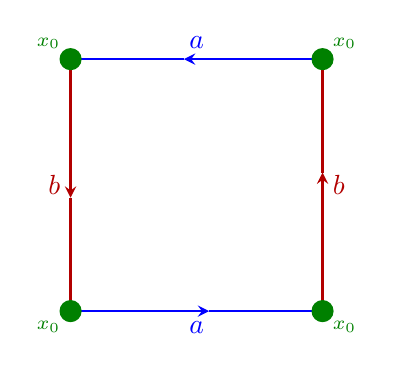
\begin{tikzpicture}[scale=1.6, >=stealth, thick]
    % Square - Torus
    \draw[->, blue] (0,0) -- (1.1,0); \draw[blue] (1.1,0) -- (2,0) node[midway, below] {};
    \node[blue, below] at (1,0) {$a$};
    \draw[->, red!70!black] (2,0) -- (2,1.1); \draw[red!70!black] (2,1.1) -- (2,2);
    \node[red!70!black, right] at (2,1) {$b$};
    \draw[->, blue] (2,2) -- (0.9,2); \draw[blue] (0.9,2) -- (0,2);
    \node[blue, above] at (1,2) {$a$};
    \draw[->, red!70!black] (0,2) -- (0,0.9); \draw[red!70!black] (0,0.9) -- (0,0);
    \node[red!70!black, left] at (0,1) {$b$};
    % Corners
    \foreach \p in {(0,0),(2,0),(0,2),(2,2)} \fill[green!50!black] \p circle (2.5pt);
    \node[below left, font=\scriptsize, green!50!black] at (0,0) {$x_0$};
    \node[below right, font=\scriptsize, green!50!black] at (2,0) {$x_0$};
    \node[above left, font=\scriptsize, green!50!black] at (0,2) {$x_0$};
    \node[above right, font=\scriptsize, green!50!black] at (2,2) {$x_0$};
\end{tikzpicture}
\end{center}

\textbf{Projective plane} ($abab$): opposite edges identified with \emph{reversed} orientation. All four corners become one point.

\begin{center}
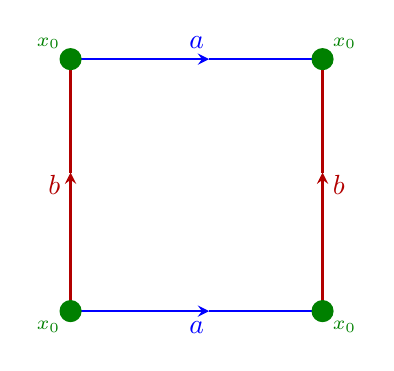
\begin{tikzpicture}[scale=1.6, >=stealth, thick]
    % Square - Projective plane
    \draw[->, blue] (0,0) -- (1.1,0); \draw[blue] (1.1,0) -- (2,0);
    \node[blue, below] at (1,0) {$a$};
    \draw[->, red!70!black] (2,0) -- (2,1.1); \draw[red!70!black] (2,1.1) -- (2,2);
    \node[red!70!black, right] at (2,1) {$b$};
    \draw[->, blue] (0,2) -- (1.1,2); \draw[blue] (1.1,2) -- (2,2);
    \node[blue, above] at (1,2) {$a$};
    \draw[->, red!70!black] (0,0) -- (0,1.1); \draw[red!70!black] (0,1.1) -- (0,2);
    \node[red!70!black, left] at (0,1) {$b$};
    % Corners
    \foreach \p in {(0,0),(2,0),(0,2),(2,2)} \fill[green!50!black] \p circle (2.5pt);
    \node[below left, font=\scriptsize, green!50!black] at (0,0) {$x_0$};
    \node[below right, font=\scriptsize, green!50!black] at (2,0) {$x_0$};
    \node[above left, font=\scriptsize, green!50!black] at (0,2) {$x_0$};
    \node[above right, font=\scriptsize, green!50!black] at (2,2) {$x_0$};
\end{tikzpicture}
\end{center}

Note: the $a$-arrows on top and bottom point in the \emph{same} direction (both left-to-right), but the top edge is traversed right-to-left when reading the boundary counterclockwise. The $b$-arrows on left and right both point \emph{upward}. This means opposite edges are identified with reversed orientation.

\textbf{Klein bottle} ($aba^{-1}b$): $a$-edges same orientation, $b$-edges reversed orientation.

\begin{center}
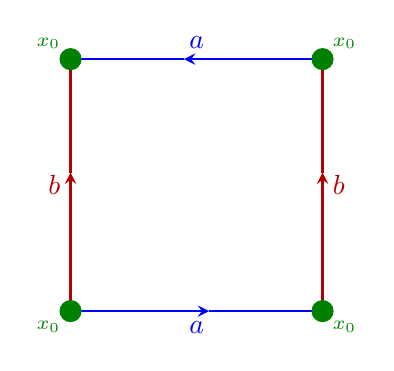
\begin{tikzpicture}[scale=1.6, >=stealth, thick]
    % Square - Klein bottle
    \draw[->, blue] (0,0) -- (1.1,0); \draw[blue] (1.1,0) -- (2,0);
    \node[blue, below] at (1,0) {$a$};
    \draw[->, red!70!black] (2,0) -- (2,1.1); \draw[red!70!black] (2,1.1) -- (2,2);
    \node[red!70!black, right] at (2,1) {$b$};
    \draw[->, blue] (2,2) -- (0.9,2); \draw[blue] (0.9,2) -- (0,2);
    \node[blue, above] at (1,2) {$a$};
    \draw[->, red!70!black] (0,0) -- (0,1.1); \draw[red!70!black] (0,1.1) -- (0,2);
    \node[red!70!black, left] at (0,1) {$b$};
    % Corners
    \foreach \p in {(0,0),(2,0),(0,2),(2,2)} \fill[green!50!black] \p circle (2.5pt);
    \node[below left, font=\scriptsize, green!50!black] at (0,0) {$x_0$};
    \node[below right, font=\scriptsize, green!50!black] at (2,0) {$x_0$};
    \node[above left, font=\scriptsize, green!50!black] at (0,2) {$x_0$};
    \node[above right, font=\scriptsize, green!50!black] at (2,2) {$x_0$};
\end{tikzpicture}
\end{center}

Note: the $a$-edges (top and bottom) have \emph{opposite} arrows (same-direction identification, like the torus). The $b$-edges (left and right) have arrows pointing the \emph{same} way (upward) --- reversed identification. This is what distinguishes the Klein bottle from the torus.

\textbf{Vertex identification:} In each case above, the edge identifications chain all four corners together: $(0,0) \sim (1,0)$ via $a$, then $(1,0) \sim (1,1)$ via $b$, then $(1,1) \sim (0,1)$ via $a$, then $(0,1) \sim (0,0)$ via $b$. So all four corners become a single point $x_0$, and the boundary $\partial P$ becomes a wedge of circles at $x_0$.
\end{exbox}

\begin{thmbox}[{Fundamental Group of a Polygonal Surface (Munkres 74.1)}]
Let $P$ be a polygonal region with labels and orientations on edges. Let $X = P/{\sim}$ be the quotient space and $\pi: P \to X$ the quotient map. If $\pi$ maps all the vertices of $P$ to a single point $x_0 \in X$, then
\[\pi_1(X, x_0) \cong \langle\, a_1, \ldots, a_k \mid w \,\rangle\]
where $a_1, \ldots, a_k$ are the distinct edge labels and $w$ is the word obtained by reading the labels around $\partial P$ once counterclockwise.
\end{thmbox}

\begin{proof}[Proof sketch]
Since $\pi$ sends all vertices to $x_0$, the image $\pi(\partial P)$ is a wedge of $k$ circles (one for each distinct label), joined at $x_0$. The loop running once around $\partial P$ counterclockwise maps to the word $w$ in these circles.

Apply van Kampen to $X = U \cup V$ where:
\begin{itemize}[nosep]
    \item $U$ = image of the interior of $P$ (open, contractible, so $\pi_1(U) = 0$).
    \item $V$ = open neighborhood of $\pi(\partial P)$, which deformation retracts onto $\partial P / {\sim}$ = wedge of $k$ circles. So $\pi_1(V) \cong \langle a_1, \ldots, a_k \rangle = F_k$ (free group).
\end{itemize}
The intersection $U \cap V$ is an open annular strip around $\pi(\partial P)$, which has $\pi_1(U \cap V) \cong \mathbb{Z}$, generated by the circle $c$ running around $\partial P$ once.

The inclusion maps:
\begin{itemize}[nosep]
    \item $i_1: \pi_1(U \cap V) \to \pi_1(U) = 0$ is trivial (sends everything to $e$).
    \item $i_2: \pi_1(U \cap V) \to \pi_1(V) \cong \langle a_1, \ldots, a_k \rangle$ sends $[c] \mapsto [\pi \circ c] = [w]$ (the boundary loop maps to the word $w$).
\end{itemize}
By van Kampen: the relation is $i_1(c) \cdot i_2(c)^{-1} = e \cdot w^{-1} = w^{-1}$, i.e., $w = e$. Therefore:
\[\pi_1(X) \cong \frac{\pi_1(U) * \pi_1(V)}{N} \cong \frac{0 * F_k}{\langle w \rangle} \cong \frac{F_k}{\langle w \rangle} = \langle\, a_1, \ldots, a_k \mid w \,\rangle.\]
\end{proof}

\begin{exbox}[Surface Fundamental Groups]
Reading off the boundary word for each surface:
\begin{center}
\small
\begin{tabular}{|c|c|c|}
\hline
\textbf{Surface} & \textbf{Boundary word} & $\pi_1$ \\
\hline
Torus $T^2$ & $aba^{-1}b^{-1}$ & $\langle a, b \mid aba^{-1}b^{-1}\rangle \cong \mathbb{Z} \times \mathbb{Z}$ \\
\hline
Projective plane $P^2$ & $abab$ & $\langle a, b \mid abab \rangle \cong \mathbb{Z}/2\mathbb{Z}$ \\
\hline
Klein bottle $K$ & $aba^{-1}b$ & $\langle a, b \mid aba^{-1}b \rangle$ (non-abelian) \\
\hline
Double torus $\Sigma_2$ & $a_1 b_1 a_1^{-1} b_1^{-1} a_2 b_2 a_2^{-1} b_2^{-1}$ & $\langle a_1, a_2, b_1, b_2 \mid a_1 b_1 a_1^{-1} b_1^{-1} a_2 b_2 a_2^{-1} b_2^{-1} \rangle$ (non-abelian) \\
\hline
\end{tabular}
\end{center}
The double torus has $\pi_1$ non-abelian, confirming the result from \S 28 (where we proved non-abelianness via covering spaces, without computing the exact group).
\end{exbox}

% %%%%%%%%%%%%%%%%%%%%%%%%%%%%%%%%%%%%%%%%%%%%%%%%%%%%%%%%%%%%%%%%%%%%%%%%%%%%
\newpage
\part*{Appendix: The Algebraic Topology Toolkit}
\addcontentsline{toc}{part}{Appendix: The Algebraic Topology Toolkit}

\section{The One Question}

The central question of algebraic topology is: \textbf{is $X$ homeomorphic to $Y$?}

The strategy: assign to each space $X$ a group $\pi_1(X)$ such that homeomorphic spaces get isomorphic groups. Then:
\[\pi_1(X) \not\cong \pi_1(Y) \implies X \not\cong Y.\]
Almost every problem in algebraic topology reduces to: \textbf{compute $\pi_1(X)$.}

\section{The Four Computation Tools}

\textbf{Tool 1: Deformation Retract (\S 26).} \textit{Simplify the space.}

If $A$ is a deformation retract of $X$, then $\pi_1(X) \cong \pi_1(A)$. Replace a complicated space with a simpler one that has the same $\pi_1$.

\textit{When to use:} The space has ``unnecessary'' parts that can be continuously collapsed onto a subspace you already understand.

\medskip

\textbf{Tool 2: Covering Spaces + Lifting Correspondence (\S 24--25).} \textit{Count the fiber.}

If $p: E \to B$ is a covering map with $E$ simply connected, then $\pi_1(B) \leftrightarrow p^{-1}(b_0)$ (bijection via lifting correspondence).

\textit{When to use:} The space is a quotient of a simply connected space. ``Unwrap'' it via the covering map.

\medskip

\textbf{Tool 3: Product Formula (\S 23).} \textit{Split into factors.}

$\pi_1(X \times Y) \cong \pi_1(X) \times \pi_1(Y)$.

\textit{When to use:} The space is a product of spaces whose $\pi_1$ you already know.

\medskip

\textbf{Tool 4: Generation Theorem / Van Kampen (\S 27, \S 29).} \textit{Decompose into open sets.}

Write $X = U \cup V$ with $U \cap V$ path-connected. The generation theorem says $\pi_1(X)$ is generated by loops in $U$ and $V$. Van Kampen gives the precise group.

\textit{When to use:} The space can be cut into two pieces whose $\pi_1$ you already know.

\section{The Decision Tree}

Given a space $X$, compute $\pi_1(X)$ by asking:
\begin{enumerate}
    \item \textbf{Is $X$ simply connected?} (Convex? Contractible?) $\Rightarrow$ $\pi_1 = 0$. Done.
    \item \textbf{Does $X$ deformation retract onto something simpler?} $\Rightarrow$ Replace $X$ with that subspace and restart.
    \item \textbf{Is $X$ a product?} $\Rightarrow$ Product formula: compute each factor separately.
    \item \textbf{Is $X$ a quotient of a simply connected space?} $\Rightarrow$ Covering space + lifting correspondence.
    \item \textbf{Can $X$ be written as $U \cup V$?} $\Rightarrow$ Generation theorem / van Kampen.
    \item \textbf{Combine tools.} Often you need several in sequence: deformation retract first, then product formula, or covering space argument then van Kampen.
\end{enumerate}

\section{Distinguishing Spaces}

Once you can compute, the contrapositive does the work. To show $\pi_1(X) \not\cong \pi_1(Y)$, find a group property one has and the other doesn't:

\begin{center}
\small
\begin{tabular}{|p{4cm}|p{6cm}|}
\hline
\textbf{Property} & \textbf{Distinguishes} \\
\hline
Trivial vs nontrivial & $S^2$ ($\pi_1 = 0$) vs $S^1$ ($\pi_1 = \mathbb{Z}$) \\
\hline
Finite vs infinite & $P^2$ ($\pi_1 = \mathbb{Z}/2\mathbb{Z}$) vs $S^1$ ($\pi_1 = \mathbb{Z}$) \\
\hline
Abelian vs non-abelian & $T^2$ ($\pi_1 = \mathbb{Z}^2$) vs $\Sigma_2$ ($\pi_1$ non-abelian) \\
\hline
Cyclic vs non-cyclic & $S^1$ ($\pi_1 = \mathbb{Z}$) vs $T^2$ ($\pi_1 = \mathbb{Z}^2$) \\
\hline
\end{tabular}
\end{center}

\section{Summary Table of Computations}

\begin{center}
\small
\begin{tabular}{|p{3.5cm}|c|p{5cm}|}
\hline
\textbf{Space} & $\pi_1$ & \textbf{Tool used} \\
\hline
$\mathbb{R}^n$, $B^n$, convex sets & $0$ & Simply connected (straight-line homotopy) \\
\hline
$S^n$ ($n \geq 2$) & $0$ & Tool 4: generation theorem + stereographic projection \\
\hline
$S^1$ & $\mathbb{Z}$ & Tool 2: covering $\mathbb{R} \to S^1$, lifting correspondence \\
\hline
$P^n$ ($n \geq 2$) & $\mathbb{Z}/2\mathbb{Z}$ & Tool 2: covering $S^n \to P^n$, fiber has 2 points \\
\hline
$T^n = (S^1)^n$ & $\mathbb{Z}^n$ & Tool 3: product formula \\
\hline
$B^2 \times S^1$ & $\mathbb{Z}$ & Tool 3: $\pi_1(B^2) \times \pi_1(S^1) = 0 \times \mathbb{Z}$ \\
\hline
$\mathbb{R}^2 \setminus \{0\}$ & $\mathbb{Z}$ & Tool 1: deformation retract onto $S^1$ \\
\hline
$\mathbb{R}^3 \setminus \{z\text{-axis}\}$ & $\mathbb{Z}$ & Tool 1: onto $\mathbb{R}^2 \setminus \{0\}$ then $S^1$ \\
\hline
Figure eight & $F_2$ (non-abelian) & Tool 4: van Kampen (or Tool 2: covering space proves non-abelian) \\
\hline
$T^2 \setminus \{pt\}$ & $F_2$ & Tool 1: deformation retract onto figure eight \\
\hline
$\Sigma_2$ (double torus) & non-abelian & Figure eight is a retract \\
\hline
\end{tabular}
\end{center}

\begin{rembox}
This table will grow as we cover more spaces and tools. Each entry represents a combination of the decision tree steps. The power of algebraic topology is that a small number of tools, applied systematically, computes $\pi_1$ for a large class of spaces.
\end{rembox}

\section{Reverse Problem: Constructing Spaces with Given $\pi_1$}

A common exam question: \emph{find a space $X$ with $\pi_1(X) \cong G$}. The strategy is to use two building blocks and two operations:

\textbf{Building blocks:}
\begin{center}
\small
\begin{tabular}{|c|c|}
\hline
\textbf{Target group} & \textbf{Space} \\
\hline
$0$ (trivial) & $\mathbb{R}^n$, $B^n$, $S^n$ ($n \geq 2$), any contractible space \\
\hline
$\mathbb{Z}$ & $S^1$ \\
\hline
$\mathbb{Z}/n\mathbb{Z}$ & $P^2$ (for $n = 2$), lens spaces, $n$-fold dunce cap \\
\hline
\end{tabular}
\end{center}

\textbf{Operations:}
\begin{center}
\small
\begin{tabular}{|c|c|c|}
\hline
\textbf{Group operation} & \textbf{Space operation} & \textbf{Effect on $\pi_1$} \\
\hline
Direct product $G \times H$ & Product $X \times Y$ & $\pi_1(X \times Y) \cong \pi_1(X) \times \pi_1(Y)$ \\
\hline
Free product $G * H$ & Wedge $X \vee Y$ & $\pi_1(X \vee Y) \cong \pi_1(X) * \pi_1(Y)$ \\
\hline
\end{tabular}
\end{center}

Multiplying by a simply connected factor does not change $\pi_1$: $\pi_1(X \times S^2) \cong \pi_1(X) \times 0 \cong \pi_1(X)$.

\begin{exbox}[Constructing Spaces]
\begin{enumerate}
    \item $\pi_1 \cong \mathbb{Z}/2\mathbb{Z} \times \mathbb{Z}/2\mathbb{Z}$: use products $\Rightarrow$ $P^2 \times P^2$. Also $P^2 \times P^2 \times S^2$ (adding a simply connected factor).
    \item $\pi_1 \cong \mathbb{Z}/2\mathbb{Z} * \mathbb{Z}/2\mathbb{Z}$: use wedge $\Rightarrow$ $P^2 \vee P^2$. Also $P^2 \vee P^2 \times S^2$ or $P^2 \vee P^2 \vee S^2$.
    \item $\pi_1 \cong \mathbb{Z} \times \mathbb{Z}$: $S^1 \times S^1 = T^2$.
    \item $\pi_1 \cong \mathbb{Z} * \mathbb{Z} = F_2$: $S^1 \vee S^1$ (figure eight).
    \item $\pi_1 \cong \mathbb{Z} \times \mathbb{Z}/2\mathbb{Z}$: $S^1 \times P^2$.
    \item $\pi_1 \cong \mathbb{Z}^3$: $T^3 = S^1 \times S^1 \times S^1$.
\end{enumerate}
\end{exbox}

\begin{rembox}[Direct Product vs.\ Free Product: The Exam Trap]
The notation matters: $\times$ (direct product, abelian) vs.\ $*$ (free product, typically non-abelian) correspond to different space constructions ($\times$ vs.\ $\vee$). On an exam, $\mathbb{Z}/2 \times \mathbb{Z}/2$ and $\mathbb{Z}/2 * \mathbb{Z}/2$ are \emph{different groups} requiring \emph{different spaces}. Always check which one is being asked for.
\end{rembox}

\end{document}
